% !TEX program = pdflatex
% !TEX encoding = UTF-8 Unicode

% Plantilla de la clase `scrbook` del paquete KOMA-script para la
% elaboración de un TFG siguiendo las directrices del la comisión del
% Grado en Matemáticas de la Universidad de Granada.

% Francisco Torralbo Torralbo
% miércoles, 29 de abril de 2020

\documentclass{scrbook}

\KOMAoptions{%
  fontsize=11pt,        % Tamaño de fuente
  paper=a4,             % Tamaño del papel
  headings=normal,      % Tamaño de letra para los títulos: small, normal, big
  % parskip=half,         % Espacio entre párrafos: full (una línea) o half (media línea)
  headsepline=false,    % Una linea separa la cabecera del texto
  cleardoublepage=empty,% No imprime cabecera ni pie en páginas en blanco 
  chapterprefix=false,  % No antepone el texto "capítulo" antes del número
  appendixprefix=false,	% No antepone el texto "Apéndice" antes de la letra
  listof=totoc,		    	% Añade a la tabla de contenidos la lista de tablas y figuras
  index=totoc,			    % Añade a la talba de contenidos una entrada para el índice
  bibliography=totoc,	  % Añade a la tabla de contenidos una entrada para bibliografía
  BCOR=5mm,           % Reserva margen interior para la encuadernación. 
                        % El valor dependerá el tipo de encuadernado y del grosor del libro.
  DIV=10,             % Cálcula el diseño de página según ciertos 
                        % parámetros. Al aumentar el número aumentamos el ancho de texto y disminuimos el ancho del margen. Una opción de 14 producirá márgenes estrechos y texto ancho.
}

% INFORMACIÓN PARA LA VERSIÓN IMPRESA
% Si el documento ha de ser impreso en papel de tamaño a4 pero el tamaño del documento (elegido en \KOMAoptions con la ocpión paper) no es a4 descomentar la línea que carga el paquete `crop` más abajo. El paquete crop se encargará de centrar el documento en un a4 e imprimir unas guías de corte. El procedimiento completo para imprenta sería el siguiente:
% 0. Determinar, según el tipo de encuadernación del documento, el ancho reservado para el proceso de encuadernación (preguntar en la imprenta), es decir, la anchura del área del papel que se pierde durante el proceso de encuadernación. Fijar la varibale BCOR de \KOMAoptions a dicho valor.
% 1. Descomentar la siguiente línea e imprimir una única página con las guías de corte
% 2. Cambiar la opción `cross` por `cam` (o `off`) en el paquete crop y volver a compilar. Imprimir el documento (las guías de corte impresas no inferfieren con el texto).
% 3. Usar la página con las guías impresas en el punto 1 para cortar todas las páginas.

% \usepackage[a4, odd, center, pdflatex, cross]{crop} % Permite imprimir el documento en un a4 (si el tamaño es más pequeño) mostrando unas guías de corte. Útil para imprenta.

% VERSIÓN ELECTRÓNICA PARA TABLETA
% Las opciones siguientes seleccionan un tamaño de impresión similar a una tableta de 9 pulgadas con márgenes estrechos. Útil para producir una versión en pdf para ser leída en una tableta en lugar de impresa.
% Para que la portada quede centrada correctamente hay que editar el
% archivo `portada.tex` y eliminar el entorno `addmargin`

% \KOMAoptions{fontsize=10pt, paper=19.7104cm:14.7828cm, twoside=false, BCOR=0cm, DIV=14}

% ---------------------------------------------------------------------
%	PAQUETES 
% ---------------------------------------------------------------------

% CODIFICACIÓN E IDIOMA
% ---------------------------------------------------------------------
\usepackage[utf8]{inputenc} 			    % Codificación de caracteres

% Selección del idioma: cargamos por defecto inglés y español (aunque este último es el idioma por defecto para el documento). Cuando queramos cambiar de idioma escribiremos:
% \selectlanguage{english} o \selectlanguage{spanish}

\usepackage[english, spanish, es-nodecimaldot, es-tabla]{babel}

% Opciones cargadas para el paquete babel:
  % es-nodecimaldot: No cambia el punto decimal por una coma en modo matemático.
  % es-noindentfirst: No sangra los párrafos tras los títulos.
  % es-tabla: cambia el título del entorno `table` de "Cuadro" a "Tabla"

% Otras opciones del paquete spanish-babel:
  \unaccentedoperators % Desactiva los acentos en los operadores matemáticso (p.e. \lim, \max, ...). Eliminar esta opción si queremos que vayan acentuados

% MATEMÁTICAS
% ---------------------------------------------------------------------
\usepackage{amsmath, amsthm, amssymb} % Paquetes matemáticas
\usepackage{mathtools}                % Añade mejoras a amsmath
\mathtoolsset{showonlyrefs=true}      % sólo se numeran las ecuaciones que se usan
\usepackage[mathscr]{eucal} 					% Proporciona el comando \mathscr para
                                      % fuentes de tipo manuscrito en modo matemático sin sobreescribir el comando \mathcal
\usepackage{subcaption}
\usepackage[ruled]{algorithm2e}  %Para crear algoritmos
% TIPOGRAFÍA 
% ---------------------------------------------------------------------
% El paquete microtype mejora la tipografía del documento.
\usepackage[activate={true,nocompatibility},final,tracking=true,kerning=true,spacing=true,factor=1100,stretch=10,shrink=10]{microtype}

% Las tipografías elegidas para el documento, siguiendo la guía de estilo de la UGR,
% son las siguientes
% Normal font: 			URW Palladio typeface. 
% Sans-serif font: 	Gill Sans
% Monospace font: 	Inconsolata
\usepackage[T1]{fontenc}
\usepackage[sc, osf]{mathpazo} \linespread{1.05}         
\usepackage[scaled=.95,type1]{cabin} % sans serif in style of Gill Sans
% Si el paquete cabin da error usar el siguiente comando en su lugar
% \renewcommand{\sfdefault}{iwona} 
\usepackage{inconsolata}

\usepackage{float} % Imagenes float (Para poner [H])
% Selecciona el tipo de fuente para los títulos (capítulo, sección, subsección) del documento.
\setkomafont{disposition}{\sffamily\bfseries}

% Cambia el ancho de la cita. Al inicio de un capítulo podemos usar el comando \dictum[autor]{cita} para añadir una cita famosa de un autor.
\renewcommand{\dictumwidth}{0.45\textwidth} 

\recalctypearea % Necesario tras definir la tipografía a usar.

\usepackage{setspace}
% TABLAS, GRÁFICOS Y LISTADOS DE CÓDIGO
% ---------------------------------------------------------------------
\usepackage{booktabs}
% \renewcommand{\arraystretch}{1.5} % Aumenta el espacio vertical entre las filas de un entorno tabular

\usepackage{xcolor, graphicx}
% Carpeta donde buscar los archivos de imagen por defecto
\graphicspath{{img/}}

% IMAGEN DE LA PORTADA
% Existen varias opciones para la imagen de fondo de la portada del TFG. Todas ellas tienen en logotipo de la universidad de Granada en la cabecera. Las opciones son las siguientes:
% 1. portada-ugr y portada-ugr-color: diseño con marca de agua basada en el logo de la UGR (en escala de grises y color).
% 2. portada-ugr-sencilla y portada-ugr-sencilla-color: portada únicamente con el logotipo de la UGR en la cabecera.
\usepackage{eso-pic}
\newcommand\BackgroundPic{%
	\put(0,0){%
		\parbox[b][\paperheight]{\paperwidth}{%
			\vfill
			\centering
      % Indicar la imagen de fondo en el siguiente comando
			\includegraphics[width=\paperwidth,height=\paperheight,%
			keepaspectratio]{portada-ugr-sencilla-color}%
			\vfill
}}}

% \usepackage{listings} % Para la inclusión de trozos de código

% CABECERAS
% ---------------------------------------------------------------------
% Si queremos modificar las cabeceras del documento podemos usar el paquete
% `scrlayer-scrpage` de KOMA-Script. Consultar la documentación al respecto.
% \usepackage[automark]{scrlayer-scrpage}

% VARIOS
% ---------------------------------------------------------------------

%\usepackage{showkeys}	% Muestra las etiquetas del documento. Útil para revisar las referencias cruzadas.

% ÍNDICE 
% Para generar el índice hay que compilar el documento con MakeIndex. Generalmente los editores se encargan de ello automáticamente.
% ----------------------------------------------------------------------
% \index{} para añadir un elemento
% \index{main!sub} para añadir un elementos "sub" bajo la categoría "main".
% \index{termino|textbf} para dar formato al número de página (negrita).
% \index{termino|see{termino relacionado}} para crear una referencia cruzada

% Ejemplo: \index{espacio homogéneo}, \index{superficie!mínima}, \index{esfera|see{espacio homogéneo}}

% Activar los siguientes comandos para generar el índice terminológico. Ver también comandos al final de este documento para incluir dicho índice en el pdf final.
% \usepackage{makeidx}
% \makeindex

% Para revisar las entradas al índice conforme las incluimos en el documento es útil el siguiente paquete. Conviene observar que mientras esté cargado no se generará el índice.
%\usepackage{showidx} % Muestra en el margen del documento las entradas añadidas al índice. Útil para revisar el documento. Si está activo el índice no se genera

% ---------------------------------------------------------------------
% COMANDOS Y ENTORNOS
% ---------------------------------------------------------------------
% Cargamos un archivo externo donde hemos incluido todos los comandos
% propios que vamos a usar en el documento.
% DEFINICIÓN DE COMANDOS Y ENTORNOS

% CONJUNTOS DE NÚMEROS

  \newcommand{\N}{\mathbb{N}}     % Naturales
  \newcommand{\R}{\mathbb{R}}     % Reales
  \newcommand{\Z}{\mathbb{Z}}     % Enteros
  \newcommand{\Q}{\mathbb{Q}}     % Racionales
  \newcommand{\C}{\mathbb{C}}     % Complejos
  
  \newcommand{\E}{\mathbb{E}}     % Esperanza
  \newcommand{\e}{\epsilon}       % Épsilon
  \newcommand{\de}{\delta}        % Delta
  \newcommand{\Pb}{\mathbb{P}}    % P Probabilidad
  
  \newcommand{\X}{\mathcal{X}}    % X caligráfica
  \newcommand{\Y}{\mathcal{Y}}    % Y caligráfica
  \newcommand{\D}{\mathcal{D}}    % D caligráfica
  \newcommand{\A}{\mathcal{A}}    % A caligráfica
  \newcommand{\Pc}{\mathcal{P}}   % P caligráfica
  \newcommand{\Hc}{\mathcal{H}}   % H caligráfica
  \newcommand{\Rh}{\hat{R}}       % R gorro
  
  
  

% TEOREMAS Y ENTORNOS ASOCIADOS

  % \newtheorem{theorem}{Theorem}[chapter]
  \newtheorem*{teorema*}{Teorema}
  \newtheorem{teorema}{Teorema}[chapter]
  \newtheorem{proposicion}{Proposición}[chapter]
  \newtheorem{lema}{Lema}[chapter]
  \newtheorem{corolario}{Corolario}[chapter]

    \theoremstyle{definition}
  \newtheorem{definicion}{Definición}[chapter]
  \newtheorem{ejemplo}{Ejemplo}[chapter]

    \theoremstyle{remark}
  \newtheorem{observacion}{Observación}[chapter]


% --------------------------------------------------------------------
% INFORMACIÓN DEL TFG Y EL AUTOR
% --------------------------------------------------------------------
\usepackage{xspace} % Para problemas de espaciado al definir comandos

\newcommand{\miTitulo}{Desarrollo de modelos de Deep Learning basados en redes neuronales recurrentes para clasificación de electrocardiogramas\xspace}
\newcommand{\miNombre}{Juan José Herrera Aranda\xspace}
\newcommand{\miGrado}{Doble Grado en Matemáticas e Ingeniería Informática}
\newcommand{\miFacultad}{Facultad de Ciencias y Escuela Técnica Superior de Ingeniería Informática y Telecomunicaciones}
\newcommand{\miUniversidad}{Universidad de Granada}
% Añadir tantos tutores como sea necesario separando cada uno de ellos
% mediante el comando `\medskip` y una línea en blanco
\newcommand{\miTutor}{
  Francisco Herrera Triguero \\ \emph{Departamento de Ciencias de la Computación e Inteligencia Artificial} 

  % Añadir tantos tutores como sea necesario. 

  \medskip
  Julián Luengo Martión \\ \emph{Departamento de Ciencias de la Computación e Inteligencia Artificial}
}
\newcommand{\miCurso}{2021-2022\xspace}

% HYPERREFERENCES
% --------------------------------------------------------------------
\usepackage{xurl}
\usepackage[pagebackref]{hyperref}
% Opciones para el paquete hyperref
%----------------------------------

\hypersetup{%
  % hidelinks,            % Enlaces sin color ni borde. El borde no se imprime
  linkbordercolor=0.8 0 0,
  citebordercolor=0 0.8 0,
  citebordercolor=0 0.8 0,
  colorlinks = true,            % Color en texto de los enlaces. Comentar esta línea o cambiar `true` por `false` para imprimir el documento.
  linkcolor = [rgb]{0.5, 0, 0}, % Color de los enlaces internos
  urlcolor = [rgb]{0, 0, 0.5},  % Color de los hipervínculos
  citecolor = [rgb]{0, 0.5, 0}, % Color de las referencias bibliográficas
	pdftitle={\miTitulo},%
	pdfauthor={\textcopyright\ \miNombre, \miFacultad, \miUniversidad},%
  pdfsubject={Trabajo de fin de Grado},%
	pdfkeywords={},%
	pdfcreator={pdfLaTeX},%
}

% Redefinición del estilo para mostrar las referencias cruzadas en la bibliografía.
\renewcommand*{\backref}[1]{}
\renewcommand*{\backrefalt}[4]{{\footnotesize [%
    \ifcase #1 No citado%
    \or Citado en pág.~#2%
    \else Citado en págs. #2%
    \fi%
]}}

% Etiquetas en español para el comando \autoref
\def\chapterautorefname{Capítulo}
\def\appendixautorefname{Apéndice}
\def\sectionautorefname{Sección}
\def\subsectionautorefname{Subsección}
\def\figureautorefname{Fig.}
\def\tableautorefname{Tabla}

\def\teoremaautorefname{Teorema}
\def\proposicionautorefname{Proposición}
\def\lemaautorefname{Lema}
\def\corolarioautorefname{Corolario}
\def\definicionautorefname{Def.}
\def\observacionautorefname{Observación}
\def\ejemploautorefname{E.j.}

% Pone automáticamente un parántesis para las ecuaciones
\def\equationautorefname~#1\null{Ec.~(#1)\null}


\begin{document}

% --------------------------------------------------------------------
% FRONTMATTER
% -------------------------------------------------------------------
\frontmatter % Desactiva la numeración de capítulos y usa numeración romana para las páginas

% \pagestyle{plain} % No imprime cabeceras

% !TeX root = ../libro.tex
% !TeX encoding = utf8

%*******************************************************
% Titlepage
%*******************************************************
\begin{titlepage}
  \AddToShipoutPicture*{\BackgroundPic}
  \phantomsection 
  \pdfbookmark[1]{Título}{title}

  % Para que el título esté centrado en la página.
  % Los valores numéricos deberán elegirse de acuerdo con el diseño de
  % página (sobre todo si se cambia la opción BCOR o DIV).
  \begin{addmargin}[2.575cm]{0cm}
  \begin{flushleft}
    \Large  
    \hfill\vfil

    \large{\textsf{\miFacultad}}
    \vfill

    {\large\textsc\miGrado} \vfill


    {\large\textsc{trabajo de fin de grado}}

    \begin{flushleft}
      \Huge
      \setstretch{0.8}
      \miTitulo
    \end{flushleft}

    \vfill\vfill\vfill\vfill

    \textsf{\normalsize{Presentado por:}}\\
    {\normalsize\textrm{\miNombre}} 
    \bigskip

    \textsf{\normalsize{Tutor:}}\\
    {\normalsize\rmfamily\miTutor}

    \bigskip
    \textsf{\normalsize{Curso académico \miCurso}}
  \end{flushleft}  
  \end{addmargin}       

\end{titlepage}   
\cleardoublepage
\endinput
                    
% !TeX root = ../libro.tex
% !TeX encoding = utf8

%*******************************************************
% Little Dirty Titlepage
%*******************************************************

\thispagestyle{empty}

\begin{center}
  \large  

  \vspace*{\stretch{1}}

  \begingroup
  \huge{\miTitulo} \\ \bigskip
  \endgroup

  \textrm{\miNombre}

  \vspace{\stretch{5}}

\end{center}  

\newpage
\thispagestyle{empty}

\hfill

\vfill

\miNombre \textit{\miTitulo}.

Trabajo de fin de Grado. Curso académico \miCurso.
\bigskip

\begin{minipage}[t]{0.25\textwidth}
  \flushleft
  \textbf{Responsable de tutorización}
\end{minipage}
\begin{minipage}[t]{0.45\textwidth}
  \flushleft
  \miTutor
\end{minipage}
\begin{minipage}[t]{0.30\textwidth}
  \flushright
  \miGrado
  \medskip

  \miFacultad
  \medskip

  \miUniversidad
\end{minipage}

\newpage
\endinput
                     
% !TeX root = ../libro.tex
% !TeX encoding = utf8
%
%*******************************************************
% Declaración de originalidad
%*******************************************************

\thispagestyle{empty}

\hfill\vfill

\textsc{Declaración de originalidad}\\\bigskip

D./Dña. \miNombre \\\medskip

Declaro explícitamente que el trabajo presentado como Trabajo de Fin de Grado (TFG), correspondiente al curso académico \miCurso, es original, entendida esta, en el sentido de que no ha utilizado para la elaboración del trabajo fuentes sin citarlas debidamente.
\medskip

En Granada a \today 
\begin{flushleft} 
Fdo: \miNombre 

\end{flushleft}

\vfill

\cleardoublepage
\endinput
   
% !TeX root = ../libro.tex
% !TeX encoding = utf8

%*******************************************************
% Dedication
%*******************************************************
\thispagestyle{empty}
\phantomsection 
\pdfbookmark[1]{Dedicatoria}{Dedicatoria}

\hfill
\vfill

\begin{flushright}
\itshape
A mi familia, en especial a mis abuelos, a mi tía Josefa y a mi tío Juanito.
\end{flushright}

\vfill

\cleardoublepage
\endinput
                % Opcional
% !TeX root = ../libro.tex
% !TeX encoding = utf8

%*******************************************************
% Table of Contents
%*******************************************************
\phantomsection
\pdfbookmark[0]{\contentsname}{toc}

\setcounter{tocdepth}{2} % <-- 2 includes up to subsections in the ToC
\setcounter{secnumdepth}{3} % <-- 3 numbers up to subsubsections

% \manualmark
% \markboth{\textsc{\contentsname}}{\textsc{\contentsname}}
\tableofcontents 

%*******************************************************
% List of Figures and of the Tables
%*******************************************************

    % *******************************************************
    %  List of Figures
    % *******************************************************    
    \phantomsection 
    % \listoffigures

    %*******************************************************
    % List of Tables
    %*******************************************************
    \phantomsection 
    % \listoftables
    
    %*******************************************************
    % List of Listings
    % The package \usepackage{listings} is needed
    %*******************************************************      
	  % \phantomsection 
    % \renewcommand{\lstlistlistingname}{Listados de código}
    % \lstlistoflistings 

\cleardoublepage
            
% !TeX root = ../libro.tex
% !TeX encoding = utf8

%*******************************************************
% Agradecimientos
%*******************************************************

\chapter{Agradecimientos}

    Este proyecto refleja el resultado de cinco arduos años de carrera, en los que en cada uno de ellos he dado lo mejor de mí. Me gustaría decir ha habido momentos duros y no tan duros, pero en verdad, todos han sido duros, sin treguas ni trincheras. Y aún así, estos años los volvería a repetir sin miramientos, la carrera en sí ha sido hermosa, pero la experiencia que me llevo, aún más. \\
    
    Primeramente, quiero hacer mención a unas personas muy especiales y que sin ellas todo habría tomado un camino distinto. Unas personas con las que el sentimiento de piña, el apoyo y las risas era nuestro día a día. Hablo de mis hermanos del \textit{Real Colegio Mayor San Bartolomé y Santiago}: Anchoa, Marrón, Hans, Tucán, Currichar, Atom y mi Gran Caimán, Ramiro (de este último no digo el mote verdadero para no tener problemas si alguien con cualquier tipo de sensibilidad lee estas líneas). Cada uno de vosotros habéis contribuido a lo que soy hoy en día y no puedo estar más orgulloso de que seáis vosotros lo que hayáis hecho esto. ¡Prometo no defraudaros!. Desde mi más profundo interior, gracias. \\
    
    Segundo, quiero agradecer a mi familia, en especial a mi padre, madre y hermano por todo lo que me han apoyado y hecho por mí. Mi madre en particular por su amor incondicional y mi padre, por su preocupación, también incondicional. Espero haceros sentir orgullosos. También quiero hacer una especial mención a mis cuatro abuelos: Vaque y Pindata y Manolo y Antonia, uno de ellos falleció estando en tercero de carrera y fue un duro golpe. También quiero dar reconocimiento a todos mis titos, en particular a mi tito Yoyo, y por supuesto a mis tíos Luis y Beli con los que siempre suelo echar un café antes de irme a Granada. Todos habéis sido indispensables para mí en estos años. Muchas gracias de corazón. \\
    
    Por úlimo agradecer a todas las persona, compañeros de clase, amigos y colegas que he conocido durante estos años y que no han hecho más que aportarme experiencias y vivencias haciéndome crecer y madurar como persona. Por último, también agradecer a una personita muy especial que conocí en tercero de carrera de la que he aprendido lecciones de vida, otra manera distinta de estudiar y de la que no dejo aún de aprender. De nuevo, gracias a todos. \\

\cleardoublepage
\endinput
            % Opcional

% \pagestyle{scrheadings} % A partir de ahora sí imprime cabeceras
% !TeX root = ../libro.tex
% !TeX encoding = utf8
%
%*******************************************************
% Summary
%*******************************************************


\chapter{Resumen}


    Aunque el documento conste de 5 partes, se puede ver como tres grandes partes: matemáticas, informática y clasificación de arritmias. La parte de matemáticas se centra en describir las bases del aprendizaje estadístico, previamente detallando los pilares del mismo para ir construyendo progresivamente esta teoría. El aprendizaje estadístico se fundamente en la probabilidad, la cual a su vez requiere de conceptos de teoría de la medida e integración. De este modo, se comienza dando unos fundamentos muy básicos sobre estas materias para introducir la probabilidad y así desembocar más tarde en la teoría del aprendizaje.\\
    
    En la teoría del aprendizaje, se verán algunos resultados que son generales, pero la mayoría del trabajo está enfocado en un caso particular y especialmente sencillo, la clasificación binaria. El objetivo será llegar hasta el teorema fundamental del aprendizaje estadístico, pero para ello se deberán detallar muchos conceptos previos. Se empezará con el aprendizaje correcto probablemente aproximado (PAC) que permite evaluar la dificultad de un problema en el contexto del aprendizaje supervisado y una generalización suya, el aprendizaje PAC agnóstico. Para esta generalización también se definirá el aprendizaje por convergencia uniforme, ya que será necesario para dar un resultado sobre las clases de hipótesis que son PAC agnósticas aprendibles. \\
    
    Continuando todavía en el marco del aprendizaje estadístico, se da un salto al estudio de las cotas de generalización que son una herramienta muy importante que miden cuan bien el modelo ha conseguido trascender el aprendizaje para lograr unos correctos resultados fuera de los datos de entrenamiento. Se clasificarán las cotas de generalización en función del conjunto de hipótesis, así se tendrán cotas de generalización para conjunto de hipótesis finitos y para conjuntos de hipótesis infinitos. Es en esta última parte donde comienza la teoría de la dimensión de Vapnik-Chervonenkis más conocida con el nombre de dimensión VC. \\
    
    La dimensión de Vapnik-Chervonenkis es de vital importancia pues hasta ahora, la clase de hipótesis que se han usado son aquellas que tienen cardinal finito. Esta teoría establece la viabilidad del aprendizaje en términos de clases de hipótesis con cardinal infinito, por lo que la gama de estos conjuntos que se pueden abarcar será mucho más grande. Un resultado importante será la cota de generalización VC. Se concluirá dicha sección con el teorema fundamental del aprendizaje estadístico el cual relaciona todos los conceptos comentados hasta ahora y da una equivalencia entre la clases de hipótesis con dimensión VC finita y las clases de hipótesis PAC aprendibles. \\

    Para terminar la parte matemática del proyecto se introducirá el teorema de aproximación universal que expone que la salida producida por una red neuronal es densa en el espacio de funciones continuas en el cubo unitario $n$-dimensional.  \\


    En la parte de informática se introducirán las redes neuronales prealimentadas junto con su proceso de entrenamiento. Tras esto, se introducen las redes neuronales convolucionales. Este tipo de redes surgieron con la finalidad de identificar patrones u objetivos en imágenes, pero también tienen una amplia aplicación en señales unidimensionales. Para terminar con la parte informática se verán las redes neuronales recurrentes (RNN). Este tipo de redes tienen la habilidad de recordar y olvidar información a lo largo del tiempo, algo que es verdaderamente útil. Hay muchos tipos de redes neuronales recurrentes, en particular esta sección se centrará en las conocidas como LSTM y GRU que resuelven un problema muy común que presentan, la dependencia a corto y largo plazo causada por el desvanecimiento y/o la explosión del gradiente.  \\
    
    En la parte de clasificación de arritmias se presenta un problema de gran relevancia en la actualidad. La arritmia supone un grave problema para la salud y en el peor de los casos, la muerte. Es una enfermedad muy presente en nuestro día a día. Los especialistas sanitarios las diagnostican analizando las señales proporcionadas por un electrocardiograma (ECG) el cual mide la actividad eléctrica del corazón. La automatización de la detección y clasificación de arritmias es algo de vital importancia no solo para los pacientes, sino también para los médicos.\\
    
    Hay dos enfoques para enfrentar este problema, el tradicional y el moderno. Es en este último enfoque en donde el aprendizaje profundo juega un papel clave y resuelve el principal inconveniente que exige el enfoque tradicional, poseer un conocimiento a priori. Para el desarrollo de esta parte se usará una base, de una competición del año 2017, para clasificar un tipo de arritmia llamada \textit{fibrilación auricular}. Los modelos a usar serán de dos tipos, los primeros son modelos ya propuestos por la literatura, los cuales se replicarán y probarán. Los segundos son un conjunto de tres propuesta propias obtenidas tras un proceso experimental. La primera propuesta consistirá en una arquitectura de red convolucional estándar sin nada que destacar. La segunda propuesta será una combinación de CNN y LSTM. La última propuesta será una variante de la segunda pero cambiando las unidades LSTM por GRU. \\
    
    Los mejores resultados son los de los modelos ganadores de la competición. Los peores resultados lo presentan aquellos modelos extraídos de la literatura por estar diseñados específicamente para tratar con otras bases de datos más o menos complejas que la empleada. Finalmente, los modelos propios, pese a no superar a los ganadores, obtuvieron buenos resultados dignos de la competición. \\
    
    \begin{center}
        \textbf{Palabras clave:}
        \begin{center}
            Fibrilación Auricular, Arritmia, Aprendizaje Profundo, Clasificación, Inteligencia Artificial, Redes Neuronales, LSTM, GRU. 
        \end{center}
    \end{center}
    


    






\endinput
 
% !TeX root = ../libro.tex
% !TeX encoding = utf8
%
%*******************************************************
% Summary
%*******************************************************

\selectlanguage{english}
\chapter{Summary}

    \begin{center}
        \textbf{Key words:}
        \begin{center}
            Atrial Fibrillation, Arrhythmia, Deep Learning, Classification, Artificial Intelligence. 
        \end{center}
    \end{center}

    Artificial intelligence has been one of the great milestones of the last century and after countless obstacles, today it is an indissoluble part of our daily lives. So much so that if it hypothetically ceased to exist, the world would collapse. Today it can be seen everywhere, autonomous driving systems, online text translators, smart watches and even in some household appliances. Artificial intelligence is not only used to provide human comfort, but also to save lives, and this is the main focus of the work. The project is based on the application of artificial intelligence, more specifically deep learning, to detect and classify a type of heart disease known as arrhythmia. \\

    Although the document has been developed in 5 parts, it can be seen as three main parts: mathematics, computer science and project development. The first two are the most theoretical, leaving the last one for practical application. The first part introduces the mathematical foundations behind machine learning. In particular, the work focuses on describing the foundations of statistical learning, previously detailing its pillars in order to progressively build this theory. Statistical learning is based on probability, which in turn requires concepts of measurement theory and integration. Thus, we begin by giving some fundamentals of analysis that are necessary in what follows. The key concepts of measure theory to build this framework will be discussed in detail below, since a measurable space with an associated measure forms what is known as a measure space, which is a particular case of a probability space. Some concepts about integration will also be of vital importance as they will be used later to explain the calculation of probabilities. \\

    After detailing the most basic pillars, the theoretical framework of modern probability will be gradually introduced. The most important idea of this theory is to model one or more random experiments in a probability space. In most cases, the observations are nondeterministic and will be encoded as measurable applications. Thus, each random observation is a measurable application and the probabilities of the entire range of possible observations will be described in terms of the distribution of the corresponding random variable. Here, the aforementioned concepts of random variable, distribution function, density function, probability mass function plus some properties will be defined. At this point, the theory of measurement is left behind because it cannot describe the structure of dependence existing between random variables and will enter fully into the theory of probability. We will begin by defining the dependence between events and end with the dependence of random variables linked to the conditional probability. Then, we will go into detail with one of the most important and fundamental concepts, the moments, in particular we will talk about hope, variance and covariance. We conclude the part of probability with one of the most relevant results in statistical learning theory, the famous Hoeffding inequality. This probabilistic inequality bounds the probability that the mean of a set of independent and identically distributed random variables deviates by more than one threshold with respect to its expectation. \\



    Having explained and understood all of the above, it is time to dive into the theory of statistical learning, we will see some general results, but most of the work is focused on a particular and especially simple case, the binary classification. We will begin by defining the concepts that make up the learning task, all with the objective of formally defining the concept of learning. Next, the performance paradigm, known as Empirical Error Minimization (ERM), will be discussed. Then the concept of Probabilistically Approximate Correct Learning (PAC) will be introduced, which allows to evaluate the difficulty of a problem in the context of supervised learning. This difficulty is evaluated at two levels, whether the learning algorithm or the hypothesis class is PAC learnable or not. Therefore, after the definition of the concept, the conditions under which a model fulfills this property will be studied. Later it will be seen that the definition of learnable CAP is not entirely general and an effort will be made to generalize it, which gives rise to the concept of agnostic CAP learning. After which we will proceed again to find the conditions under which a model is CAP agnostic and for this purpose we will resort to the concept of learning by uniform convergence. \\
    
    Continuing still in the framework of statistical learning, a leap is made to the study of generalization levels. Generalization scores are a very important tool that measure how well your model has managed to transcend learning to achieve correct results outside the training data. We will classify the generalization scores according to the hypothesis set, so we will have generalization scores for finite hypothesis sets, distinguishing two cases, the consistent and the inconsistent; and for infinite hypothesis sets, and it is in this part where the Vapnik-Chervonenkis dimension theory, better known as VC dimension, begins. \\
    
    To go into this theory we will first define some key concepts such as dichotomy, growth function and breakpoints. The concept of VC dimension will then be defined. The study of learnable PAC models was carried out for those with finite hypothesis classes, however, when the hypothesis class is infinite, it is at this point when the VC dimension is used, since infinite hypothesis sets with finite VC dimension can exist, which allows the study of a wide range of models. Furthermore, it will be seen that when the VC dimension is infinite, then the model will not be PAC learnable, so the object of study will now focus on those models with finite VC dimension regardless of the cardinal of the hypothesis class. After the staging of this theoretical framework, we continue by detailing the generalization dimension for infinite hypothesis class known as the VC dimension. This quotient is one of the most important mathematical results in statistical learning theory for establishing the feasibility of learning with infinite set of hypotheses and for being a universal result, being understood that it is applicable to any learning algorithm, any set of hypotheses, etc. This section will conclude with the fundamental theorem of statistical learning, which relates all the concepts discussed so far. \\
    
    VC analysis shows that the choice of a hypothesis has to strike a balance between approximation to the target function within the training data and generalization to the new data. Another viewpoint that addresses this is the approximation-generalization trade-off, which is based on the decomposition of the expectation of the squared error into two terms known as bias and variance. \\
    
    To conclude the mathematical part of the project, the universal approximation theorem will be introduced, which states that the output produced by a neural network is dense in the space of continuous functions in any compact interval. In other words, we can approximate any continuous function in a compact space by means of neural networks. This result is supported by two important theorems of functional analysis: the Hanh-Banach theorem and the Riesz representation theorem. \\
    
    
    
    The second part of the project has a theoretical computer science approach with the objective of understanding the mechanisms applied in the third part of the project, which is based on the elaboration of Deep Learning models based on convolutional neural networks and LSTM to solve a problem. This part will begin with a brief state of the art of neural networks. Then we will introduce the pre-fed neural networks and the notation to be used will be fixed. Neural networks are so broad that they have not been covered in their entirety, but one of the most important parts, training, has not been omitted either. Having said that, we will detail the training process, which consists of two stages. The first one is called forward propagation, in which the loss function is calculated. This stage is so named because the weights of one layer influence the weights of the next layer, causing the propagation to advance in the direction of the first layers towards the last ones. The second stage is called back propagation and is where the well-known Back-Propagation algorithm is applied. In this stage the gradient of the loss function is calculated as a function of the weights. The name of this stage is due to the fact that in the calculation of the gradient is advanced from the last layers to the first ones. After the gradient calculation, the optimization method known as downward gradient, which has many variants, is applied. Another key aspect of neural networks is the type of activation function thanks to which a non-linearity contribution to the output is achieved, the most common activation functions used today will be discussed and compared with each other, in addition to mentioning disadvantages and disadvantages.
    
    
    After knowing the modus operandis of pre-fed neural networks, convolutional neural networks are introduced, which are simply the previous ones but including a set of new layers, not only neurons. This type of networks emerged with the purpose of identifying patterns or targets in images, but they also have a wide application in one-dimensional signals. Pre-powered neural networks have the disadvantage that if they operate with images, the amount of weights that the network needs to train increases considerably, making them not very functional. Convolutional networks solve this and other problems. To understand the operation of these networks, we must first understand the convolution operation and how it works. Basically it consists of sliding a filter over the input performing basic operations. Once this is understood, the layers that exist in this type of networks will be presented. We will talk about convolutional layers and some of their properties such as local connectivity, spatial arrangement and the implications of sharing parameters. The role and usefulness of pooling layers and normalization layers will also be discussed, and this section will end with a brief explanation of the design patterns of these network architectures. \\
    
    To conclude the second part of this project, we will look at a type of neural networks that is quite important for the third part, recurrent neural networks (RNN). These types of networks exhibit behavior that is somewhat intelligent in that they have the ability to remember and forget information over time, which is really useful. There are many types of recurrent neural networks, in particular this section will focus on those known as LSTM which is a variation of this type of networks that solve a very common problem they have, and the short and long term dependence caused by gradient fading and/or bursting. The structure of an LSTM cell is quite curious, it is formed by a set of gates, which are nothing more than an activation function with an associated operation (addition or multiplication) that perform different tasks. For example, one gate is in charge of what to forget, another one decides what to remember, another one is in charge of putting together the current knowledge with what to forget and what to remember. GRUs are another type of recurrent neural networks, similar to LSTMs but with a different structure. This concludes the second part of the project. \\
    
    
    
    The third part of the project culminates with the development of the practical part where a problem of great relevance today is presented. Arrhythmia is a disease caused by an irregular heartbeat, which is a serious health problem and in the worst case, death. This pathology does not understand gender, it affects men and women equally and although it is present in older individuals, it can also be found in the young population. Health specialists diagnose arrhythmia by analyzing the signals provided by an electrocardiogram (ECG) which measures the electrical activity of the heart. Automating the detection and classification of arrhythmias is of vital importance not only for patients, but also for physicians. \\
    
    The traditional approach to this problem has been for researchers to extract signal features manually. This has a drawback, which is that a priori medical knowledge is required, increasing the level of difficulty. With the development of deep learning in recent years, this was no longer a problem, as it was the model itself that was responsible for extracting the features it saw fit. It is this latter approach to which the work is devoted. For the experimentation we used a database of a competition carried out by the PhysioNet platform in which the objective was to classify a type of arrhythmia called \textit{atrial fibrillation}. The models that have been used to classify arrhythmias are of two types, the first are models already proposed by the literature, which have been replicated and tested. The second type is a set of three proprietary proposals obtained after an experimental process. The first proposal consisted of a standard convolutional network architecture with nothing to highlight. The second proposal was a combination of CNN and LSTM. The last proposal is a variant of the second one but changing the LSTM units for GRU. \\
    
    As expected, the best results were those of the winning models of the competition. The worst results were presented by those models extracted from the literature for a simple reason, overfitting. This is because these models had many more degrees of complexity than the data required, thus overfitting to the peculiarities of the inherent noise. In the end, the in-house models, while not outperforming the winners, performed well enough to compete. \\



% Al finalizar el resumen en inglés, volvemos a seleccionar el idioma español para el documento
\selectlanguage{spanish} 
\endinput
              

% --------------------------------------------------------------------
% MAINMATTER
% --------------------------------------------------------------------
\mainmatter % activa la numeración de capítulos, resetea la numeración de las páginas y usa números arábigos

\setpartpreamble[c][0.75\linewidth]{%
	\bigskip % Deja un espacio vertical en la parte superior
}
\part{Introducción y objetivos} % Dividir un libro en partes OPCIONAL
% !TeX root = ../libro.tex
% !TeX encoding = utf8
%
%*******************************************************
% Introducción
%*******************************************************

% \manualmark
% \markboth{\textsc{Introducción}}{\textsc{Introducción}} 

\chapter{Introducción}

De acuerdo con la comisión de grado, el TFG debe incluir una introducción en la que se describan claramente los objetivos previstos inicialmente en la propuesta de TFG, indicando si han sido o no alcanzados, los antecedentes importantes para el desarrollo, los resultados obtenidos, en su caso y las principales fuentes consultadas.

Ver archivo \texttt{preliminares/introduccion.tex}

\endinput

% !TeX root = ../libro.tex
% !TeX encoding = utf8

\setchapterpreamble[c][0.90\linewidth]{%
	\sffamily
  
	\par\bigskip
}

\chapter{Objetivos}\label{ch:objetivos}

    Los objetivos planteados al inicio del trabajo son los siguientes:
    
    \begin{itemize}
        \item Matemáticas: Se busca entender el funcionamiento y potencial de las redes profundas, para lo cual se busca:
            \begin{enumerate}
                \item Estudiar los conceptos matemáticos en los que se fundamentan
                \item Analizar algunos resultados sobre las redes neuronales
            \end{enumerate}
            
        \item Informática: Se busca abordar un problema de clasificación de señales de ECG para lo cual se busca:
            \begin{enumerate}
                \item Elaboración de modelos de aprendizaje profundo basados en redes neuronales recurrentes para la clasificación de arritmias.
                \item Estudiar y reproducir algunos modelos destacables de la literatura y realizar una comparación con los ya propuestos.
            \end{enumerate}
    \end{itemize}

    Los objetivos de la parte de matemáticas han sido cubiertos:
    \begin{enumerate}
        \item El primer objetivo queda cubierto por los capítulos \ref{ch:FundamentosMatematicos}, \ref{ch:DesigualdadHoeffding} y \ref{ch:AprendizajeEstadistico} en los que se estudia la teoría del aprendizaje estadístico que es en la que se fundamenta el aprendizaje automático, así como el aprendizaje profundo.
        \item El segundo objetivo queda cubierto por el capítulo \ref{ch:TAUniversal} en el que se presenta un importante teorema sobre la salida de las redes neuronales.
    \end{enumerate}
    
    Los objetivos de la parte de informática también han sido cubiertos:
    \begin{enumerate}
        \item El primer objetivo ha sido cubierto por los capítulos \ref{ch:descripcion_problema}, \ref{ch:contexto_experimental}, \ref{ch:desarrollo} y \ref{ch:analisis}.
        \item El segundo objetivo queda cubierto por los capítulos \ref{ch:desarrollo} y \ref{ch:analisis}.
    \end{enumerate}





    


\endinput




\setpartpreamble[c][0.75\linewidth]{%
	\bigskip % Deja un espacio vertical en la parte superior
  El propósito del capítulo es exponer los fundamentos matemáticos del Machine Learning, para ello se empezará desde los más básicos resultados de matemáticas en lo que respecta análisis y probabilidad. Tras ello, se expondrá la teoría del aprendizaje estadístico y el capítulo se finalizará con un resultado que garantiza la factibilidad del uso de redes neuronales para problemas de aprendizaje.
}
\part{Fundamentos Matemáticos} % Dividir un libro en partes OPCIONAL

% !TeX root = ../libro.tex
% !TeX encoding = utf8

\setchapterpreamble[c][0.75\linewidth]{%
	\sffamily
 
    
   En este capítulo vamos a presentar los conceptos y teoremas clave que fundamentan la teoría de lo que sigue. Empezaremos viendo de manera superficial el concepto de diferenciabilidad para continuar con la regla de la cadena y una discusión extendida sobre la confusión que da lugar el actual abuso de notación cometido por ingenieros y físicos. Estos resultados los usaremos para explicar más adelante el algoritmo de BackPropagation. La probabilidad surge de manera natural con con el concepto de medida y junto a este se encuentra el concepto de integral respecto de una medida. Así pues, daremos una pincelada sobre los aspectos necesarios dentro de la teoría de la medida exponiendo los conceptos que nos van a hacer falta como por ejemplo, lo que es un espacio medible, una medida, un espacio de medida y aplicaciones medibles. Posteriormente se darán algunos resultados sobre integración para poder adentrarnos poco a poco en el mundo de la probabilidad y sus resultados más relevantes. Una vez dentro de la parte de probabilidad se verán los aspectos más básicos de esta teoría como las variables aleatorias junto con algunos de sus resultados más importantes. También se estudiarán las distribuciones de probabilidad, función masa de probabilidad y función de densidad junto con algunos aspectos destacables. También se verá el concepto de independencia tanto para eventos como para variables aleatorias y el concepto de distribución de probabilidad condicionada junto con algunos resultados relativamente importantes como lo es la fórmula de la suma y la fórmula de Bayes. Por último se presentarán los momentos de una variable aleatoria haciendo especial incapié en la esperanza, la varianza y la covarianza.\\ 
   
   
   La referencia empleadas para la elaboración de este capítulo han sido \cite{probcourse}, \cite{probreal}, \cite{FJP}y \cite{Rohatgi2000}
	\par\bigskip
}

\chapter{Fundamentos Matemáticos}\label{ch:FundamentosMatematicos}

%%%%%%%%%%%%%%%%%%%%%%%%%%%%%%%%%%%%%%%%%%%%%%%%%%%%%%%%%%%%%%%%%%%%%%%%%%%%%%%%%%%%%%%%%
%%%%%%%%%%%%%%%%%%%%%%%%%%%%%%%%%%%%%%%%%%%%%%%%%%%%%%%%%%%%%%%%%%%%%%%%%%%%%%%%%%%%%%%%%
%%%%%%%%%%%%%%%%%%%%%%%%%%%%%%%%%%%%%%%%%%%%%%%%%%%%%%%%%%%%%%%%%%%%%%%%%%%%%%%%%%%%%%%%%

\newpage 
\section{Fundamentos del Análisis}

\subsection{Diferenciabilidad}

    \begin{definicion}[Derivada direccional de un campo escalar]
    Sea $f$ un campo escalar definido en un conjunto abierto  $\Omega \subset \R^n$, sea $a \in \Omega$ y $u$ una dirección. Se define la derivada de $f$ en $a$ en la dirección $u$ como el límite
    
    \begin{equation}
        D_{u}f(a) = \underset{t \to 0}{\lim} \frac{f(a + tu) - f(a)}{t}
    \end{equation}
    \end{definicion}

    \begin{definicion}[Diferenciabilidad de campos escalares]
    Sea $f$ un campo escalar definico en un abierto $\Omega \subset \R^n$ y sea $a \in \Omega$. Supongamos que está definido el vector gradiente $\nabla f(a)$. Se dice que $f$ es diferenciable o derivable en $a$ si se verifica que,
    
    \begin{equation}
        \underset{x \to a}{\lim} \frac{f(x) - f(a) - \langle \nabla f(a) | x - a \rangle}{||x - a||} = 0
    \end{equation}
    \end{definicion}
    
    Cuando la derivada sea en la dirección del vector $e_k$ de la base canónica, se llamará derivada parcial de primer orden de $f$ en $a$ respecto de la variable k-esima. \\
    
    \begin{proposicion}
    Sea $f$ un campo escalar diferenciable en un punto $a$ y sea $u$ una dirección en $\R^n$. entonces se verifica que,
    \begin{equation}
        D_{u} f(a) = \langle \nabla f(a) | x \rangle
    \end{equation}
    \end{proposicion}
    
    \begin{teorema}[Condición suficente de diferenciabilidad para campos escalares]
    Un campo escalar que tiene derivadas parciales continuas en un conjunto abierto es diferenciable en todo punto de dicho conjunto
    \end{teorema}

    \begin{definicion}[Diferenciabilidad de campos vectoriales]
    Sea $F:\Omega \to \R^m$ un campo vectorial donde $\Omega \subset \R^n$ es un abierto y sea $a \in \Omega$. Se dice que $F$ es diferenciable o derivable en $a$ si existe una aplicación lineal $T:\\R^n \to \R^m$ tal que
    \begin{equation}
        \underset{x \to a}{\lim} \frac{F(x) - F(a) - T(x - a)}{||x - a||} = 0
    \end{equation}
    \noindent Dicha aplicación lineal, si existe es única y se llama diferencial o derivada de $F$ en el punto $a$ y se representa por $DF(a)$
    \end{definicion}
    
    \begin{proposicion}
    Sea $F = (f_1,...,f_m): \Omega \to \R^m$ donde $\Omega \subset \R^n$ es un abierto, una función vectorial de $n$ variables y $m$ componentes. equivalen las siguientes afirmaciones
    \begin{enumerate}
    \item F es diferenciable en a
    \item Los campos escalares $f_i, i=1,...,m$ componentes de F son diferenciables en $a$    
    \end{enumerate}
    \end{proposicion}
    
    Supuesto que se verifiquen 1) y 2), la matriz de la aplicación lineal DF(z) en las bases canónicas de $\R^n$ y $\R^m$ es la matriz cuyas filas son los vectores gradiente $\nabla f_i(a)$, esto es la matriz de $m$ filas y $n$ columnas $\Big(D_j f_i(a)\Big)_{1 \leq i \leq m}^{1 \leq j \leq n}$. Esta matriz recibe el nombre de matriz jacobiana de $F$ en $a$ y se representará por $J_F(a)$

\subsection{Regla de la Cadena para el Calculo de Derivadas}
    
    La regla de la cadena se usa para calcular las derivadas de una función compuesta por otras funciones. Vamos a enunciar dos teoremas, el primero es la regla de la cadena para funciones que toman valores en la recta real y el segundo es una generalización del primero, dirigido a funciones que toman valores en $\mathbb{R}^n$ con $n$ un número natural arbitrario. 
        
            \begin{teorema}[Regla de la cadena - caso unidimensional]
                Sean $\Omega_1$ y $\Omega_2 \subset \mathbb{R}$ dos abiertos y sean $f:\Omega_2 \rightarrow \mathbb{R}$ y $g:\Omega_1 \rightarrow \mathbb{R}$ dos funciones derivables en los puntos $x_0$ y $g(x_0)$ respectivamente y verificando que $g(\Omega_1) \subset \Omega_2$ (i.e. la composición $f\circ g$ está bien definida). Entonces la composición $h = f\circ g$ es derivable en $x_0$ y se verifica que $$h'(x_0) = (f(g(x_0)))' = f'(g(x_0))g'(x_0)$$
                
                Además, si las funciones $f$, y $g$ son de clase $\mathcal{C}^k$ entonces $h$ también lo será.
            \end{teorema}
        
        La notación para la derivada usada en el anterior teorema es conocida como la notación de Lagrange, pero de aquí en adelante nos va a interesar más usar la famosa notación de Leibniz. Por lo que vamos a escribir el resultado anterior con esta nueva notación. Para ello, consideramos $x \in \Omega_2$ que sería nuestro $x_0$ y ahora llamamos $y = g(x)$ y $z = f(g(x))$, entonces se tiene que $$\frac{\partial z}{\partial x} = \frac{\partial z }{\partial y}\frac{\partial y}{\partial x}$$ \\
        
            \begin{teorema}[Regla de la cadena - caso n-dimensional]
             Sean $\Omega_1 \subset \mathbb{R}^q$ y $\Omega_2 \subset \mathbb{R}^n$ dos abiertos y sean $F:\Omega_2 \rightarrow \mathbb{R}^m$ y $G:\Omega_1 \rightarrow \mathbb{R}^n$ dos funciones diferenciables en los puntos $x_0 \in \Omega_1$ y $G(x_0)$ respectivamente y verificando que $G(\Omega_1) \subset \Omega_2$. Entonces se verifica que la función compuesta $H = F\circ G: \Omega_1 \rightarrow \mathbb{R}^m$ es diferenciable en $x_0$ y su diferencial viene dada como la composición de las respectivas diferenciales: 
             \begin{equation}\label{eq:CR2}
                DH(a) = DF(G(a)) \circ DG(a)
             \end{equation}
              
             
             Además, si las funciones $F$, y $G$ son de clase $\mathcal{C}^k$ entonces $H$ también lo será. 
            \end{teorema}
            
        Observamos que $DG(a):\mathbb{R}^q  \rightarrow \mathbb{R}^n$ y $DF(G(a)): \mathbb{R}^n \rightarrow \mathbb{R}^m$, por lo que la composición es una aplicación lineal de $\mathbb{R}^q$ a $\mathbb{R}^m$, como debe ser, pues $H$ es una función vectorial de $q$ variables y $m$ componentes. \\
        
        \noindent La expresión de la igualdad \eqref{eq:CR2} usando matrices jacobianas es:
        
        \begin{equation}
            J_H(a) = J_{F}(G(a)) \cdot J_{G}(a)
        \end{equation}
        
        \noindent Tanto $F$, como $G$ y $H$ son campos vectoriales, por tanto, para ${y = (y_1,...,y_q) \in \mathbb{R}^q}$, ${x = (x_1,...,x_n) \in \mathbb{R}^n}$ se tiene que:
        
        \begin{equation}
            \begin{aligned}
            & (x_1,...,x_n) \mapsto F(x_1,...,x_n) = (f_1(x_1,...,x_n),...,f_m(x_1,...,x_n)) \\
            & (y_1,...,y_q) \mapsto G(y_1,...,y_q) = (g_1(y_1,...,y_q),...,g_n(y_1,...,y_q)) \\
            \end{aligned}
        \end{equation}
        
        \noindent siendo $f_j$ y $g_i$ con $1 \leq i \leq q$ y $1 \leq j \leq n$ los respectivos campos escalares, entonces
                
        \begin{equation}
            \begin{aligned}
            & (y_1,...,y_q) \mapsto H(y_1,...,y_q)  = F\Big(g_1(y_1,...,y_q),...,g_n(y_1,...,y_q))\Big) \\
            & = \Bigg(f_1\Big(g_1(y_1,...,y_q),...,g_n(y_1,...,y_q)\Big),..., f_m\Big(g_1(y_1,...,y_1),...,g_n(y_1,...,y_q)\Big)\Bigg)
            \end{aligned}
        \end{equation}
        
        \noindent Poniendo ahora $H=(h_1,...,h_m)$ y escribiendo $b = G(a)$ tenemos que:
        
        \begin{equation}\label{eq:ReglaCadena}
            \frac{\partial h_i}{\partial y_j}(a) = \sum_{k=1}^{n} \frac{\partial f_i}{\partial x_k}(b)\frac{\partial g_k}{\partial y_j}(a) \qquad b = G(a) \qquad (1 \leq i \leq m, 1 \leq j \leq q )
        \end{equation}
         
         Esta igualdad constituye la regla de la cadena para derivadas parciales. Lo más habitual es que $F$ sea un campo escalar. Supongamos, pues, que en lo anterior, $F=f$ es un campo escalar, en cuyo caso $h=f \circ G$ también es un campo escalar. La igualdad \eqref{eq:ReglaCadena} queda ahora:
         
         \begin{equation}\label{ed:RC campo escalar}
             \frac{\partial h}{\partial y_j}(a) = \sum_{k=1}^{n} \frac{\partial f}{\partial x_k}(b)\frac{\partial g_k}{\partial y_j}(a) \qquad b = G(a) \qquad (1 \leq j \leq q )
         \end{equation}
         
        \noindent Podemos interpretar esta igualdad como que la función $G:\Omega_1 \rightarrow \Omega_2 \subset \mathbb{R}^n$  hace un \textit{cambio de variables}, es decir, que las \textit{variables antiguas}  de la función $f$, esto es $x=(x_1,...,x_n) \in \Omega_2$, se han sustituido por \textit{variables nuevas} $y=(y_1,...,y_q) \in \Omega_1$ y la función $f$ se ha \textit{expresado en estas nuevas variables} dando lugar a la función $h$. La relación entre unas variables y otras viene dada por $x_k = g_k(y_1,...,y_q)$ con $1 \leq k \leq n$. \\  
         
         Según comenta Javier Pérez en su libro \textit{Cálculo diferencial de funciones de varias variables} \cite{FJP}, ocurre que en muchos textos y libros comenten un abuso de notación para facilitar los cálculos pero que puede llegar a confusión, vamos a detallarlo un poco ya que más adelante nosotros también cometeremos ese abuso. Primeramente, se suele identificar a las funciones $g_k$ que introducen las nuevas coordenadas con las coordenadas antiguas $x_k$, es decir, vemos la coordenadas antiguas como funciones de las nuevas y esto lo escribimos de la siguiente forma.
         
         \begin{equation}
             x_k = x_k(y_1,...,y_q) \qquad 1 \leq k \leq n
         \end{equation}
         
         \noindent Con esta notación la igualdad \eqref{ed:RC campo escalar} queda como sigue:
         
         \begin{equation}
             \frac{\partial h}{\partial y_j}(a) = \sum_{k=1}^{n} \frac{\partial f}{\partial x_k}(b)\frac{\partial x_k}{\partial y_j}(a) \qquad b = G(a) \qquad (1 \leq j \leq q )
         \end{equation}
         
         \noindent La letra $x_k$ juega un doble papel, cuando se deriva con respecto a ella representa una variable y cuando ella se deriva respecto de una variable nueva representa una función. \\
         
         Otro abuso de notación muy común que se comete y que resulta bastante peligroso es identificar la función $f$ y $h$ como si fueran la misma con la excusa de que son la misma función expresada en distintas variables. Identificando además la función con una letra, $z$ tenemos que 
         
         \begin{equation}
             \frac{\partial z}{\partial y_j}(a) = \sum_{k=1}^{n} \frac{\partial z}{\partial x_k}(b)\frac{\partial x_k}{\partial y_j}(a) \qquad b = G(a) \qquad (1 \leq j \leq q )
         \end{equation}
         
         \noindent Aquí, la variable $z$ juega un doble papel, a la izquierda representa una función compuesta $h$ y a la derecha es la función dada en sus variables iniciales $f$. \\
         
         Es muy importante entender la relación entre los puntos $a$ y $b$ ya que hay que saber los puntos en los que se evalúan las derivadas. En casi todos los libros de ingenierías y física, esta última parte se omite, por lo que nosotros también lo haremos, por lo que finalmente nos queda:
         
         \begin{equation}
             \frac{\partial z}{\partial y_j} = \sum_{k=1}^{n} \frac{\partial z}{\partial x_k}\frac{\partial x_k}{\partial y_j}  \qquad (1 \leq j \leq q )
         \end{equation}
         
         \noindent que expresado de manera vectorial
         
         \begin{equation}
            \nabla_{y}z = \left(\frac{\partial x}{\partial y}\right)^T \nabla_{x}z
         \end{equation} 
         
         
         La notación como más adelante veremos, simplificará mucho los cálculos. Sin embargo, puede llevar a grandes confusiones si no se tiene claro en todo momento qué representa cada variable y los puntos en los que se evalúa la derivada. \\

\subsection{Conceptos básicos sobre Teoría de la Medida}
    
    
    Empezaremos primeramente introduciendo el pilar en el que se sustenta la teoría de la probabilidad, que es su estructura algebraica, así pues presentaremos el concepto de $\sigma$-algebra, que formará junto con el conjunto al cual esté asociado, un espacio medible. Cuando a estos dos ingredientes le asociamos una medida, ya tendremos la mezcla perfecta para introducir lo que se conoce como un espacio de medida, y en particular, un espacio de probabilidad. También introduciremos otros conceptos y resultados sobre aplicaciones medibles que serán el punto de partida de la siguiente sección.
    
       

    \begin{definicion}[$\sigma-algebra$]\label{def:sigma}
        Sea $\Omega$ un conjunto no vacío. Una $\sigma$ álgebra en $\Omega$ es una familia $\mathcal{A} \subset \mathcal{P}(\Omega)$ (partes de $\Omega$) que verifica:
            
        \begin{enumerate}
                \item $\Omega \in \mathcal{A}$ 
                \item Cerrado para complementario: $A \in \mathcal{A} \Rightarrow \Omega\backslash A \in \mathcal{A}$ 
                \item Cerrado para unión numerable: $A_n \in \mathcal{A} \quad \forall n \in \mathbb{N} \Rightarrow \cup^{\infty}_{n=1} \in \mathcal{A}$
        \end{enumerate}
    \end{definicion}
        
    Notamos que la primera condición es equivalente a que $\emptyset \in \mathcal{A}$ ya que $\Omega \setminus \Omega = \emptyset$. A los elementos de $\mathcal{A}$ se le llaman \textit{conjuntos medibles} y la tupla $(\Omega,\mathcal{A})$ \textit{espacio medible}.
    
     \begin{ejemplo}~\smallskip
       \begin{enumerate}
           \item $\mathcal{A} = \{\Omega, \emptyset\}$ es la $\sigma$-algebra trivial.
           
           \item La familia de las partes de $\Omega$ es la $\sigma$-algebra más grande que existe sobre $\Omega$.
           
           \item La intersección de $\sigma$-algebras es otra $\sigma$-algebra.
           
           \item La familia formada con todos los intervalos acotados de $\mathbb{R}^n$ es una $\sigma$-algebra y se le conoce como $\sigma$-algebra de Lebesgue, sobre ella se establece la medida de Lebesgue, $\lambda^n$. 
           
           \item Cualquier espacio topológico con la $\sigma$-algebra generada por la familia de abiertos de la topología es un espacio medible. En particular, la $\sigma$-algebra generada por la familia de abiertos de $\mathbb{R}^n$, que corresponde con los intervalos acotados, se la conoce como $\sigma$-algebra de Borel en $\mathbb{R}^n$. La cual se denota por $\mathcal{B}(\mathbb{R})^n$
       \end{enumerate}
    \end{ejemplo}
    
    Nosotros estamos especialmente interesados en los $\sigma$-algebras generados por una topología. Aquella que juega el rol más importante es la topología euclídea de $\mathbb{R}^n$. 
    
    \begin{teorema}[$\sigma$-algebra generada por un conjunto de subconjuntos]
    Sea $\Omega$ un conjunto no vacío arbitrario y $G \subset \mathcal{P}(\Omega)$ una familia de subconjuntos de $\Omega$. Entonces existe un $\sigma$-álgebra, $\sigma(\mathcal{G})$, que contiene a $\mathcal{G}$ y es mínima entre todas las $\sigma$-álgebras que contienen a G. Su expresión viene dada por
    $$\sigma(\mathcal{G}) := \bigcap_{\substack{ \mathcal{G} \subset \mathcal{A} \\ \mathcal{A} \subset \mathcal{P}(\Omega) \; es \; \sigma-algebra }} \mathcal{A} $$
    
    \end{teorema}
    
    \begin{definicion}[Topología]
        Sea $\Omega$ un conjunto arbitrario no vacío. Una clase de conjuntos $\tau \subset \mathcal{P}(\Omega)$ es una topología en $\Omega$ cuando cumple las siguientes propiedades:
        \begin{enumerate}
            \item $\emptyset , \Omega \in \tau$.
            \item Cerrado para intersecciones finitas: $A \cap B \in \tau$ para todo $A,B \in \tau$ 
            \item Cerrado para uniones arbitrarias: $(\cup_{A \in \mathcal{F}}A) \in \tau$ para todo $\mathcal{F} \subset \tau$.
        \end{enumerate}
    \end{definicion}
    
    Al par $(\Omega,\tau$) se le llama espacio topológico y a los conjuntos de $\tau$ se conocen como abiertos, los complementarios de los abiertos se llaman cerrados. A diferencia de una $\sigma$-álgebra, las topologías son cerradas para intersecciones finitas, pero también son cerradas para uniones arbitrarias. Vamos a dar un ejemplo de la $\sigma$-algebra de Borel que es la mínima $\sigma$-algebra que contiene una topología dada.
    
        \begin{ejemplo}~\smallskip
           Sea $(\Omega, \tau)$ un espacio topológico. La $\sigma$-álgebra $$\mathcal{B}(\Omega) := \mathcal{B}(\Omega,\tau):=\sigma(\tau)$$ que es generada por los conjuntos abiertos se llama $\sigma$-algebra de Borel en $\Omega$. Los elementos de $\mathcal{B}(\Omega,\tau)$ son llamados conjuntos de Borel o conjuntos Borel medibles. Frecuentemente la topología que se usa es la usual de $\mathbb{R}^n$
        \end{ejemplo}   
    
    
    
    \begin{definicion}[Medida]\label{def:medida}
          Sea $(\Omega,\mathcal{A})$ un espacio medible. Una medida en $(\Omega,\mathcal{A})$ es una aplicación $\mu: \mathcal{A} \rightarrow \mathbb{R}_0^+$ tal que
                  
          \begin{enumerate}
             \item $\mu(\emptyset) = 0$
             \item Si $\{A_m\}_{n\in\mathbb{N}} \subset \mathcal{A}$ es una colección numerable de subconjuntos tales que ${A_i \cap A_j = \emptyset}$ para $i\not=j$, entonces $\mu(\cup^{\infty}_{n=1}A_n) = \sum^{\infty}_{n=1} \mu(A_n)$
          \end{enumerate}
     \end{definicion}
     
     
     Gracias a las definiciones \ref{def:sigma} y \ref{def:medida} podemos presentar lo que se conoce como espacio de medida, que no es más que un espacio medible con una medida asociada al $\sigma$-algebra, $(\Omega,\mathcal{A},\mu)$. Ahora bien, el objetivo es introducir lo que viene a ser un espacio de probabilidad, que es un caso particular de espacio de medida en el que la imagen de $\mu$ está restringida al intervalo $[0,1]$ y $\mu(\Omega)=1$. Pero antes de ello, veamos algunos ejemplos.
     
     
    \begin{ejemplo}~\smallskip
       \begin{enumerate}
           \item Sea $\omega \in \Omega$ y $\delta_{\omega}(A) = \mathbb{I}_A(\omega)$, donde $\mathbb{I}_A(\omega)$ es la función indicadora para un $\omega$,  entonces $\delta_{\omega}$ es una medida de probabilidad para cualquier $\sigma$- álgebra, se la conoce como \textit{medida de Dirac} 
           
           \item Existe una medida unívocamente determinada, $\lambda^n$ en $(\mathbb{R}^n,\mathcal{B}(\mathbb{R}^n))$ con la siguiente propiedad,
           $$\lambda^n((a,b]) = \prod_{i=1}^n(b_i-a_i)$$
           para todo $a,b \in \mathbb{R}^n$ con $a<b$. Esta medida se la conoce como la medida de Lebesgue  en $(\mathbb{R}^n,\mathcal{B}(\mathbb{R}^n))$ o también como la medida de Lebesgue-Borel.
           
           \item La restrición de la medida de Lebesgue-Borel de $(\mathbb{R},\mathcal{B}(\mathbb{R}))$ a $[0,1]$ es una pedida de probabilidad en $([0,1],\mathcal{B}(\mathbb{R})|_{[0,1]})$
       \end{enumerate}
       \end{ejemplo}
     
     
    \begin{definicion}[Espacio de probabilidad]
        Un espacio de probabilidad es una terna $(\Omega,\mathcal{A},P)$ donde $\Omega$ es un conjunto llamado espacio muestral que contiene a todos los posibles resultados del experimento. $\mathcal{A}$ es una $\sigma$-álgebra asociada a $\Omega$ y ${P:\mathcal{A}\rightarrow [0,1]}$ es una función de probabilidad que asigna una probabilidad a todo suceso verificando los tres axiomas de Kolmogorov
        
        \begin{itemize}
            \item $P(\Omega)=1$
            \item $P(A) \geq 0 \quad \forall A \in \mathcal{A}$
            \item Si $\{A_m\}_{n\in\mathbb{N}} \subset \mathcal{A}$ es una colección numerable de subconjuntos tales que ${A_i \cap A_j = \emptyset}$ para $i\not=j$, entonces $P(\cup^{\infty}_{n=1}A_n) = \sum^{\infty}_{n=1} P(A_n)$
        \end{itemize}
      \end{definicion}
      
      Vamos a introducir a continuación la definición de aplicación medible. Es de vital importancia no confundir el concepto de medida con el de aplicación medible, ya que no tienen nada que ver.
      
      \begin{definicion}[Aplicación medible]
      Sean $(\Omega_1,\mathcal{A}_1)$ y $(\Omega_2,\mathcal{A}_2)$ dos espacios medibles. Una aplicación $X:\Omega_1 \rightarrow \Omega_2$ se dice que es medible cuando la imagen inversa por $X$ de todo elemento de $\mathcal{A}_2$ es un elemento en $\mathcal{A}_1$, esto es, $X^{-1}(A) \in \mathcal{A}_1$ para todo $A \in \mathcal{A}_2$. Cuando $X$ sea medible, escribiremos $X:(\Omega_1,\mathcal{A}_1) \rightarrow (\Omega_2,\mathcal{A}_2)$
      \end{definicion}
      
      Hemos definido el concepto de aplicación medible sobre un espacio medible de forma general. En lo que nos atañe podemos usar otra definición de manera más particular, para ello fijamos un conjunto medible $\Omega \subset \mathbb{R}^n$, consideramos un espacio topológico $Y$ y entonces diremos que $f:\Omega \to Y$ es una función medible cuando la imagen inversa por $f$ de todo subconjunto abierto de $Y$, sea un conjunto medible, es decir,
      $$O = O^{\circ} \subset Y \implies f^{-1}(G) \in \mathcal{M}$$ donde $\mathcal{M}$ es la familia de todos los subconjuntos medibles de $\mathbb{R}^n$ \\ 
      
      A modo de ejemplo, podemos ver muy fácilmente que toda función continua $g:\Omega \to Y$ es medible, ya que dado un abierto $O \subset Y$, se tiene que $h^{-1}(O)$ es abierto en $\Omega$, es decir, $h^{-1}(G) = A \cap \Omega$ donde $A$ es un abierto de $\mathbb{R}^n$, luego $h^{-1}(G)$ es medible, por serlo $A$ y $\Omega$
       
      \begin{observacion}
      El concepto de medibilidad es una propiedad muy débil. De hecho, si no aplicamos el axioma de elección, es imposible probar la existencia de conjuntos que no sean medibles, por lo que para cualquier espacio topológico $Y$, tampoco se puede probar la existencia de una función de $\Omega$ en $Y$ que no sea medible. En la práctica, cualquier función que tenga una definición explícita, que no involucre de alguna forma el axioma de elección, va a ser medible.
      \end{observacion}
      
   
       
    \begin{ejemplo}~\smallskip
       \begin{enumerate}
       
            \item La identidad es una aplicación medible 
            \item La composición de aplicaciones medibles es medible
            \item La función indicadora de un subconjunto $A \subset \Omega$ se define como 
           $$ \mathbb{I}_{A}(\omega):= \left\{ \begin{array}{lcc} 1 & si & \omega\in A\\
           \\ 0 & si & \omega \notin A \end{array} \right. $$
           y es una aplicación medible en el espacio $(\Omega, \mathcal{A})$ si y sólo si $A \in \mathcal{A}$
           
           \item Cualquier aplicación $X:(\Omega,\mathcal{P}(\Omega))\to(\Omega',\{\emptyset, \Omega'\})$, donde $\mathcal{P}(\Omega)$ representa las partes de $\Omega$, es medible
       \end{enumerate}
     \end{ejemplo} 
       
      
%%%%%%%%%%%%%%%%%%%%%%%%%%%%%%%%%%%%%%%%%%%%%%%%%%%%%%%%%%%%%%%%%%%%%%%%%%%%%%%%%%%%%%%%%
%%%%%%%%%%%%%%%%%%%%%%%%%%%%%%%%%%%%%%%%%%%%%%%%%%%%%%%%%%%%%%%%%%%%%%%%%%%%%%%%%%%%%%%%%
%%%%%%%%%%%%%%%%%%%%%%%%%%%%%%%%%%%%%%%%%%%%%%%%%%%%%%%%%%%%%%%%%%%%%%%%%%%%%%%%%%%%%%%%%
     
\subsection{Resultados sobre integración}

    Basándonos en las nociones de espacios de medida y aplicaciones medibles, introducimos la integral de una aplicación medible con respecto a una medida general. Esto generaliza la integral de Lebesgue. Además, se introducirán algunos resultados clave que serán usados en la siguiente sección. \\ 

    Vamos a partir de un espacio de medida $(\Omega, \mathcal{A}, \mu)$ y una función real medible ${f:\Omega \to \mathbb{R} \cup \{-\infty,\infty\}}$, con estos elementos se puede definir el concepto de integral de una función medible real respecto de la medida $\mu$ y cuya expresión viene dada por
    $$\int f(\omega)\mu(d\omega) := \int_{\Omega} f \; d\mu$$ \\
    
    Esta integral se construye primeramente para las llamadas funciones simples positivas, dicha construcción se extiende a funciones medibles positivas como el límite de dichas funciones y posteriormente a las funciones medibles. Diremos que $f$ es $\mu$-integrable cuando la integral de $f$ respecto de una medida $\mu$ exista, es decir, cuando $\int_{\Omega}|f| d\mu < \infty$. Veamos algunas de sus propiedades y resultados más relevantes, pero previamente definimos el espacio de las funciones medibles $\mu$-integrables como 
    
    $$\mathcal{L}^1(\mu):= \mathcal{L}^1(\Omega, \mathcal{A}, \mu) := \Bigl\{ f:\Omega \to \mathbb{R}\cup\{-\infty,\infty\}: f \; es \; medible \; y \; \int_{\Omega} |f| d\mu < \infty \Bigl\}$$
    
    \begin{proposicion}[Propiedades]
    Sea $f,g \in \mathcal{L}^1(\mu)$
    \begin{enumerate}
        \item (Monotonía) Si $f\leq g$ casi por doquier, entonces $\int f d\mu \leq \int g d\mu$. En particular, si $f=g$ c.p.d.\footnote{c.p.d. son las siglas de casi por doquier. Una propiedad se cumple casi por cuando se cumple siempre exceptuando un conjunto de medida nula} entonces $\int f d\mu = \int g d\mu$
        \item (Desigualdad Triangular) $ |\int f d\mu| \leq \int |f| d\mu$
        \item (Linealidad) Si $\alpha, \beta \in \mathbb{R}$, entonces $\alpha f + \beta g \in \mathcal{L}^1(\mu)$ y 
        $$ \int (\alpha f + \beta g) \; d\mu = \alpha \int f \; d\mu + \beta \int g \; d\mu $$
    \end{enumerate}
    \end{proposicion}
    
    \begin{proposicion}
    Sea $f:\Omega \to [0,\infty]$ una aplicación medible, entonces:
    \begin{enumerate}
        \item $f=0$ c.p.d. si y solo si $\int f d\mu = 0$
        \item Si $\int_{\Omega} f d\mu < \infty$ entonces $f < \infty$ c.p.d.
    \end{enumerate}
    \end{proposicion}
    
    Los siguientes teoremas y proposiciones nos van a ser útiles a la hora de calcular más adelante la esperanza y los momentos de orden superior de una variable aleatoria.
    
    \begin{proposicion} \label{prop:int1}
    Sean $(\Omega, \mathcal{A})$ y $(\Omega', \mathcal{A}')$ dos espacios medibles. Sea $\mu$ una medida en $\Omega$ y sea $X:\Omega \to \Omega'$ una aplicación medible. Definimos $\mu_X = \mu \circ X^{-1}$, que es una medida en $(\Omega',\mathcal{A}')$. Sea $f:\Omega' \to \Bar{\mathbb{R}}$ $\mu_X$-integrable en $\Omega'$. Entonces $f \circ X \in \mathcal{L}^1(\mu)$ y $$\int_{\Omega} (f \circ X) \; d\mu = \int_{\Omega'} f \; d(\mu \circ X^{-1})$$
    \end{proposicion}
    
    \begin{definicion}
        Sea $(\Omega, \mathcal{A}, \mu)$ un espacio de medida y $f:\Omega \to [0,\infty)$ una función medible. Definimos $v:\mathcal{A} \to \mathbb{R}$ como $$v(A) := \int_A f \; d\mu := \int_\Omega (f\mathbb{I}_A) \; d\mu, \quad \forall A \in \mathcal{A} $$
    \end{definicion}    
    
    Se tiene que $v$ es una medida en $\Omega$. Escribiremos $f\mu = v$ y diremos que $v$ tiene una función de densidad $f$ respecto de $\mu$. En el caso de que $\mu$ sea la medida de Lebesgue se dirá directamente que $v$ tiene función de densidad $f$. Un detalle muy importante es que bajo las condiciones de la definición anterior, tenemos que la función de densidad $f$ respecto de $\mu$ es única. \\ 
    
    
    \begin{proposicion} \label{prop:int2}
     Sea $(\Omega, \mathcal{A}, \mu)$ un espacio de medida. Sea $f:\Omega \to [0,\infty]$ y $g:\Omega \to \bar{\mathbb{R}}$ funciones medibles. Entonces $g$ es $f\mu$-integrable en $\Omega$ si y solo si $gf$ es $\mu$-integrable en $\Omega$, en cuyo caso
     $$\int_{\Omega} g \; d(f\mu) = \int_{\Omega} gf \; d\mu$$
    \end{proposicion}


%%%%%%%%%%%%%%%%%%%%%%%%%%%%%%%%%%%%%%%%%%%%%%%%%
%%%%%%%%%%%%%%%%%%%%%%%%%%%%%%%%%%%%%%%%%%%%%%%%%
%%%%%%%%%%%%%%%%%%%%%%%%%%%%%%%%%%%%%%%%%%%%%%%%%

\section{Fundamentos de Probabilidad}       

    Una vez expuestas las nociones básicas de medida juntos con los resultados de integración nos adentramos en la teoría de la probabilidad. La idea fundamental de la teoría de la probabilidad moderna es modelar uno o varios experimentos aleatorios como un espacio de probabilidad $(\Omega,\mathcal{A},P)$. Los conjuntos $A \in \mathcal{A}$ se denominan sucesos. En la mayoría de los casos, los eventos de $\Omega$ no se observan directamente. Más bien, las observaciones son aspectos de los experimentos individuales que se codifican como aplicaciones medibles de $\Omega$ a un espacio de posibles observaciones. En resumen, cada observación aleatoria en una aplicación medible y las probabilidades de las posibles observaciones aleatorias se describirán en términos de la distribución de la variable aleatoria correspondiente.\\
    

\subsection{Variables Aleatorias}

    En este capítulo expondremos el concepto de variable aleatoria, tanto para casos continuos y discretos junto con el concepto de función de distribución. Aunque nos centraremos en las variables aleatorias con valores reales que son las que nos interesan de cara a la teoría del aprendizaje. También detallaremos teoremas y conceptos clave relacionados entre sí para forjar las bases de cara a los siguientes capítulos.\\
    
    
        \begin{definicion}[Variable Aleatoria]\label{def:VA}
            Sea $(\Omega, \mathcal{A},P)$ un espacio de probabilidad y $(\Omega',\mathcal{A}')$ un espacio medible. Decimos que $X:\Omega \to \Omega'$ es una variable aleatoria con valores en $\Omega'$ si $X$ es una aplicación medible, esto es,
            \begin{equation}\label{eq:defVA}
            X^{-1}(B) = \{\omega \in \Omega: X(\omega) \in B\} \in  \mathcal{A} \quad \forall B \in \mathcal{A}'
            \end{equation}
        \end{definicion}        
        
    
    En particular, si ($\Omega',\mathcal{A}') = (\mathbb{R},\mathcal{B}(\mathbb{R}))$ decimos que $X$ es una variable aleatoria real. Para verificar que una aplicación es una variable aleatoria real no es necesario comprobar que se cumple la definición para todo conjunto boleriano. Bastaría comprobarlo para un generador de $\mathcal{B}(\mathbb{R})$, nosotros vamos a usar la clase de intervalos cerrados por la derecha de la forma $(-\infty,x]$ con $x \in \mathbb{R}$. \\
    
    Otro caso particular que también tiene especial relevancia es cuando $\Omega' = \mathbb{R}^n$ y $\mathcal{A}' = \mathcal{B}(\mathbb{R}^n)$, en cuyo caso tendremos que $X$ es un vector aleatorio real o una variable aleatoria N-dimensional. Démosle una definición
    
        \begin{definicion}[Vector Aleatorio Real]\footnote{Pueden darse definiciones parecidas del concepto de vector aleatorio, en términos de intervalos de cualquier otro tipo}
            Dado un espacio de probabilidad $(\Omega, \mathcal{A}, P)$, se llama vector aleatorio (n-dimensional) a toda aplicación
     
                
                \begin{align}
                    \mathbf{X} = (X_1,...,X_2): \; & \Omega \to \mathbb{R}^n &\\
                    & \omega \mapsto \mathbf{X}(\omega) = (X_1(\omega),...,X_n(\Omega))
                \end{align}
                
            que cumpla,
            $$\mathbf{X}^{-1}((-\infty,\mathbf{x}]) \in \mathcal{A} \quad \forall \mathbf{x} \in \mathbf{R}^n$$
        \end{definicion}
        
    Ni que decir tiene que dado un vector aleatorio $\mathbf{X}$ la aplicación $X_i = \Pi_i \circ \mathbf{X}$ obtenida de proyectar el vector aleatorio en su componente i-ésima es una aplicación medible, por lo que cada componente del vector aleatorio es una variable aleatoria. Incluso se podría establecer una caracterización y decir que $\mathbf{X}$ es un vector aleatoria si y solo si todas sus componentes son vectores aleatorios. \\
    
    Bajo el pretexto de la definición \ref{def:VA}, si $X(\Omega)$ es un conjunto numerable, diremos que $X$ es una variable aleatoria discreta. En otro caso, será una variable aleatoria continua. A partir de ahora vamos a considerar como espacio de probabilidad $(\Omega, \mathcal{A},P)$. \\
    
        \begin{teorema}[Caracterización Variable Aleatoria Real]
        $X$ es una V.A.\footnote{V.A. denota Variable Aleatoria} real si y solo si para cada $x \in \mathbb{R}$ 
            \begin{align}
                \{\omega: X(\omega)\leq x\} = \{X \leq x\} \in \mathcal{A}
            \end{align}
        
        \end{teorema}
    
        \begin{observacion}
        \begin{enumerate}
            \item Si $X$ es una V.A. real los conjuntos $\{X = x\}$, $\{a < X \leq b$\},${\{X < x\}}$,$\{a \leq X < b\}$, $\{a < X < b\}$ y $\{a \leq X \leq b\}$ son todos eventos. Además podemos usar cualquiera de estos intervalos para definir una variable aleatoria.
        \end{enumerate}
        \end{observacion}
    
        \begin{proposicion}
        Sea $X$ una variable aleatoria real definida en un espacio de probabilidad y sea $g$ una función medible. Entonces $Y=g(X)$ es una variable aleatoria
        \end{proposicion}
        
        La demostración de esta proposición es bastante sencilla y se apoya en el hecho de que la composición de funciones medibles es medible. Con esta proposición podemos transformar una V.A. en otra sin más que componerla con cualquier función medible. 
    
        \begin{ejemplo}
        Sea $\Omega = \{ HH,TT,HT,TH \}$ y $\mathcal{A}$ las partes de $\Omega$. Definimos $X$ por
        $$X(\omega) = "Numero \; de \; H's \; en \; \omega"$$
        Por lo que $X(HH) = 2$,$X(HT)=1$,$X(TH)=1$,$X(TT)=0$
        
        $$ X^{-1}(-\infty,x] = \left\{ 
        \begin{array}{lcc} 
                \emptyset &   x<0, \\
                \\ \{TT\}  & 0 \leq  x < 1, \\
                \\ \{TT,HT,TH\} & 1 \leq x < 2, \\
                \\ \Omega & 2 \leq x
        \end{array} \right. $$
        Por lo que X es una V.A. real. 
        \end{ejemplo}
    
    Notamos que no hemos usado la noción de probabilidad en la definición de V.A. Esta noción entra en juego para definir la llamada distribución de probabilidad. De manera intuitiva, como $P$ es una medida de probabilidad sobre $(\Omega, \mathcal{A})$, sabemos calcular probabilidades en $\Omega$ vía $P$. Al tener una aplicación medible $X:\Omega \to \Omega'$ vamos a tener una forma de medir en $\Omega'$. Entonces la medida de probabilidad $P$ sobre $(\Omega, \mathcal{A})$ induce una nueva medida de probabilidad sobre $\Omega'$ que da lugar a la siguiente definición. \\
    
   
    
    \begin{definicion}[Distribución de Probabilidad]
            Sea $(\Omega, \mathcal{A}, P)$ un espacio de probabilidad y $(\Omega',\mathcal{A}')$ un espacio medible. Sea $X:\Omega \to \Omega'$ una V.A.
        \begin{enumerate}
        
            \item Definimos la distribución de X como $P_X = P \circ X^{-1}$, que es una medida de probabilidad. Renombrando $\mu = P_X$ escribiremos $X \sim \mu$ y diremos que $X$ sigue o tiene una distribución $\mu$.
                
            \item Para variables aleatorias reales $X$, la función $F_X: \mathbf{X}(\Omega) \subset \mathbb{R} \to [0,1]$ dada por ${ F_X(x) = P_X((-\infty,x]) = P(X^{-1}\{(-\infty,x]\}) = P[\omega \in \Omega: X(\omega) \leq x] = P[X \leq x]}$ se llama función de distribución de X.
                
            \item En el caso $(\Omega', \mathcal{A}')=(\mathbb{R}^n,\mathcal{B}(\mathbb{R}^n)$ se define la función $F_X: \mathbf{X}(\Omega) \subset \mathbb{R}^n \to [0,1]$ como, 
                
                $$F_X(x) = P[\mathbf{X} \leq \mathbf{x}] = P_X(]-\infty,\mathbf{x}]^n)$$ y se le llama función de distribución de $P_X$.
                
            Las distribuciones de cada una de las variables aleatorias que componen el vector reciben el nombre de distribuciones marginales y la función de distribución marginal viene dada por
            
            $$F_{X_i} = \lim_{\substack{x_j \to \infty \\ i \neq j }} F_X(x_1,...,x_i,...,x_n)$$
                
            \item Una familia $(X_i)_{i \in I}$ de variables aleatorias se dice que son idénticamente distribuidas cuando $P_{X_i} = P_{X_j}$ para todo $i,j \in I$ y se denota como $X_i \overset{\mathcal{D}}{=} X_j$
        \end{enumerate}
        
    \end{definicion}
    
    \begin{proposicion}[Caracterización de una función de distribución]~\smallskip
    Una función de distribución acumulada $F(x)$ asociada a la variable aleatoria real $X$  satisface:
    \begin{enumerate}
        \item $F$ es monótona no decreciente, i.e., si $x_1 < x_2$ entonces $F(x_1) < F(x_2)$
        \item $F$ es continua por la derecha, i.e., $\lim_{x \to a^+}F(x) = F(a^+)$
        \item $0 \leq F(x) \leq 1 \quad \forall x \in X(\Omega)$
        \item $\lim_{x \to + \infty}F(x) = 1$
        \item $\lim_{x \to -\infty}F(x) = 0$
    \end{enumerate}
    
    \end{proposicion}
    
    \begin{teorema}
    Para cada función de distribución $F$, existe una variable aleatoria real $X$ tal que $F_X = F$
    \end{teorema}
    
    \begin{definicion}[Función masa de probabilidad]
        Sea $(\Omega, \mathcal{A}, P)$ un espacio de probabilidad y sea $X:\Omega \to \mathbb{R}$ una variable aleatoria discreta. Se define la \textit{función masa de probabilidad de X}, $p_X:X(\Omega) \to [0,1]$ como sigue
        $$p_X(x) = P_X(x) = P([X=x]) \quad \forall x \in X(\Omega)$$
        
        Si $\mathbf{X}$ fuera un vector aleatorio que toma valores en $\mathbb{R}^n$ entonces,
        $$p_X(x) = P[\mathbf{X} = x] = P[X_1 = x_1,...,X_n = x_m] \quad \forall x \in \mathbf{X}(\Omega)$$
        y se dirá que $p_X$ es la función masa de probabilidad conjunta
    
    \end{definicion}
    
    \begin{definicion}[Función de densidad]
    Sea $(\Omega, \mathcal{A}, P)$ un espacio de probabilidad y sea $X:\Omega \to \mathbb{R}$ una variable aleatoria continua tal que $F_X$ tiene densidad $f_X$ respecto de la medida de Lebesgue en $\mathbb{R}$. A la función $f_X:X(\Omega) \to \mathbb{R}$ se le conoce como la \textit{función de densidad de X}, y cumple,
    $$F_X(x) = P[X \leq x] = \int_{-\infty}^x f_X(s) \; ds \quad \forall x \in X(\Omega)$$
    
    Si $\mathbf{X}$ fuera un vector aleatorio con valores en $\mathbb{R}^n$ entonces,
    
    $$F_X(x) = P[X_1 \leq x_1,...,X_n \leq x_n] = \int_{-\infty}^{x_n} ... \int_{-\infty}^{x_1} f_X(s_1,...,s_n) \; ds \quad \forall x = (x_1,...,x_n) \in X(\Omega)$$
    \end{definicion}
    
    \begin{proposicion}[Propiedades f.d. y f.m.p.]~\smallskip
    \begin{enumerate}
        \item La función masa de probabilidad de una V.A. $X$ cumple:
        \begin{enumerate}
            \item $p_X(x) \geq 0 \quad \forall x \in X(\Omega)$
            \item $\sum_{x\in X(\Omega)}p_X (x) = 1$
        \end{enumerate}
        \item La función de densidad de una V.A. $X$ cumple:
        \begin{enumerate}
            \item $f_X(x) > 0 \quad \forall x \in X(\Omega)$
            \item $\int_{-\infty}^{+\infty} f_X(s) \; ds = 1$
        \end{enumerate}
    \end{enumerate}
    
    \end{proposicion}
    
    A nosotros nos interesan las distribuciones de probabilidad $P_X$ en $\mathbf{R}^n$ que son absolutamente continuas respecto a la medida de Lebesgue. En este caso, el teorema de \textit{Radon-Nikodym} \cite{probcourse} nos asegura que existe una función $f:\mathbb{R}^n \to \mathbf{R}_0^+$ tal que $P_X = f \lambda^n$. \\
    
    
    Tras presentar todo lo anterior, veamos ahora un par de ejemplos de distribuciones bastante conocidas, en el caso discreto será la distribución binomial y en el caso continuo la distribución normal.
    
    \begin{ejemplo}
    Sea $p \in [0,1]$ y $n \in \mathbf{N}$ y sea $X:\Omega \to \{1,...,n\}$ una V.A. tal que 
    $$P[X=k] = \binom{n}{k} p^k (1-p)^{n-k}$$
    La distribución $P_X =: P \circ X^{-1}$ se la conoce como \textit{distribución binomial} con parámetros $n$ y $p$, y se denota por $B(n,p)$. La función de distribución viene dada por 
    $$F_X(x) = \sum_{k=0}^x  \binom{n}{k} p^k (1-p)^{n-k}$$
    \end{ejemplo}


    \begin{ejemplo}
     Sea $\mu \in \mathbb{R}$ y $\sigma^2 > 0$ y sea $X$ una variable aleatoria real con 
     $$P[X \leq x] = \frac{1}{\sqrt{2 \pi \sigma^2}} \int_{-\infty}^x exp \Big(-\frac{(t - \mu)^2}{2 \sigma^2}\Big) \; dt \quad \forall x \in \mathbb{R}$$
     La distribución de probabilidad $P_X$ se la conoce con el nombre de \textit{distribución Normal} con parámetros $\mu$ y $\sigma^2$ y se suele denotar como $\mathcal{N}_{\mu,\sigma^2}$. En particular la distribución $\mathcal{N}_{0,1}$ es la conocida como distribución normal estándar
    \end{ejemplo}
     
     
    \begin{definicion}[Convergencia en probabilidad]
        Sea $X:\Omega \to \R$ una variable aleatoria real. Sea $(X_n)_{n\in \N}$ una familia de variables aleatorias reales. Decimos que la secuencia $(X_n)_{n\in \N}$ converge en probabilidad a la variable aleatoria $X$ cuando 
            \begin{equation}
                P[|X_n - X| < \epsilon] \xrightarrow{n\rightarrow\infty} 0
            \end{equation}  

    \end{definicion}
       
      
\subsection{Independencia y Probabilidad Condicionada}

    La teoría de la medida no puede describir la estructura de dependencia que puede existir entre los eventos o las variables aleatorias. En este punto dejamos atrás la teoría de la medida para adentrarnos con más profundidad en la teoría de la probabilidad, donde definimos la independencia de los sucesos y variables aleatorias. La independencia es una noción fundamental de la teoría de la probabilidad y el cálculo de las dependencias es una de las principales tareas de la teoría, así también ocurre con la conocida probabilidad condicionada. En lo que sigue vamos a considerar que $(\Omega,\mathcal{A},P)$ es un espacio de probabilidad y los conjuntos $A \in \mathcal{A}$ como eventos.\\
    
    
    \begin{definicion}[Independencia de eventos]
        Sea $I$ un conjunto de índices arbitrarios y sea $(A_i)_{i\in I}$ una familia arbitraria de eventos. Dicha familia de eventos es independiente cuando para cualquier subconjunto finito de índices $J \subset I$ se verifica
        $$ P[ \bigcap_{j \in J} A_j] = \prod_{j \in J} P[A_j] $$
        donde P es una medida de probabilidad.
    \end{definicion}    
    
    
    \begin{definicion}[Independencia de variables aleatorias]
     Sea  $I = \{1,...,n\}$ un conjunto finito de índices y $\{ (\Omega_i,\mathcal{A}_i) : i \in I \}$ una familia finita de espacios medibles. Para cada $i\in I$ sea $X_i:\Omega \to \Omega'$ una V.A. Diremos que la familia $(X_i)_{i \in I}$ de variables aleatorias es independiente cuando verifique
     $$ F_X(x_1,...,x_n) = \prod_{i=0}^n F_{X_i}$$
    \end{definicion}
    
    
    \begin{definicion}[Probabilidad condicionada para eventos]\label{def:PCE}
    Sea $B \in \mathcal{A}$ un evento. Se define la probabilidad condicionada dado B para cualquier $A \in \mathcal{A}$ como
    
    $$ P[A|B] = 
        \left\{
            \begin{array}{cc}
                \frac{P[A \cap B]}{P[B]} &  P[B] > 0  \\
                0 & P[B] = 0 
            \end{array} 
        \right.$$
    
    \end{definicion}
      
     \begin{proposicion}{
     Dado $A,B \in \mathcal{A}$ equivalen las siguientes afirmaciones:
     \begin{enumerate}
         \item $A$ y $B$ son independientes
         \item $P[A|B] = P[A]$
         \item $P[B|A] = P[B]$
     \end{enumerate}
     }\end{proposicion}
      
    \begin{proposicion}
    Bajo el pretexto de la definición \ref{def:PCE}, $P[\cdot | B]$ es una medida de probabilidad en $(\Omega,\mathcal{A})$
    \end{proposicion}

    La proposición anterior es reveladora ya que al tener una probabilidad condicionada como medida de probabilidad, podemos considerar un espacio probabilístico con dicha probabilidad condicionada asociada, dando lugar a la distribuciones de probabilidad condicionadas. \\
    
    Realicemos la construcción, para ello trasladamos el concepto de probabilidad condicionada para eventos a variables aleatorias reales. Para ello consideramos dos V.A. $X,Y:\Omega \to \mathbb{R}$. Para cada $y \in Y(\Omega)$ y $\epsilon > 0$ suponemos que el intervalo $(y-\epsilon,y+\epsilon) \subset Y(\Omega)$ y que la probabilidad $P[y-\epsilon < Y \leq y+\epsilon]$ no sea nula. Para cada $x \in X(\Omega)$ consideramos la expresión 
    $$ P[X \leq x | y - \epsilon < Y \leq y + \epsilon] = \frac{P[X \leq x , y - \epsilon < Y \leq y + \epsilon]}{P[y-\epsilon < Y \leq y+\epsilon]} $$
    
    Dicha expresión se la conoce como la \textit{distribución de $X$ dado que $Y \in ]y - \epsilon, y + \epsilon [$}.
    
    \begin{definicion}[Distribución de Probabilidad Condicionada] \label{def:DPB}
    Sean $X,Y$ dos V.A. reales. Se define la \textit{función de distribución de $X$ condicionada a que $Y=y$} como el siguiente límite siempre y cuando exista:
    \begin{equation}\label{eq:limitProbCond}
    F_{X|Y}(x|y) = \lim_{\epsilon \to 0+}P[X \leq x | y - \epsilon < Y \leq y + \epsilon]
    \end{equation}
    \end{definicion}
    
    Conociendo la función de distribución conocemos la distribución de la variable aleatoria. Ahora bien, sabemos que esta puede ser continua o discreta, definamos a continuación la función masa de probabilidad y de densidad para distribuciones condicionadas. \\
    
    \begin{definicion}[Función de densidad de probabilidad condicionada]
    
        Bajo el pretexto de la definición \ref{def:DPB} suponiendo que las dos V.A. son continuas, definimos la \textit{función de densidad de $X$ condicionada a $Y=y$}, $f_{X|Y}(x|y)$, como una función integrable no negativa que satisface
        $$F_{X|Y} = \int_{-\infty}^x f_{X|Y}(t|y) \;dt \quad \forall x \in \mathbb{R} $$
    
    \end{definicion}    
    
    Supongamos que $(X,Y)$ es un vector aleatorio real continuo, nuestro objetivo es escribir la función de densidad de X condicionado a Y en función de la función de densidad conjunta y de la función de densidad de Y. Para ello, supongamos que la función de densidad de $P_{(X,Y)}$ es $f_{(X,Y)}$ y que la función de densidad de $P_Y$ es $f_Y$. Obviamente, dichas funciones han de ser continuas por ser funciones de densidad. Sí que hemos de suponer que $f_Y > 0$. En este caso tenemos que 
    
    \begin{equation}
        \begin{aligned}
            F_{X|Y}(x|y) & = \lim_{\epsilon \to 0+} \frac{P[X \leq x , y - \epsilon < Y \leq y + \epsilon]}{P[y-\epsilon < Y \leq y+\epsilon]}\\
            & = \frac{\int_{-\infty}^x \Big[ \int_{y - \epsilon}^{y + \epsilon}f(u,v) \; dv \Big] \; du}{\int_{y - \epsilon}^{y + \epsilon} f_2(v) \; dv} \cdot \frac{\frac{1}{ \epsilon}}{\frac{1}{\epsilon}}
        \end{aligned}
    \end{equation}
    
    \noindent tomando límite obtenemos que 
    
    \begin{equation}
        \begin{aligned}
            F_{X|Y}(x|y) = \frac{ \int_{-\infty}^{x}f(u,v) \; du}{ f_2(v) \; dv} = \int_{-\infty}^{x} \Big[ \frac{f(u,y)}{f_2(y)} \Big]
        \end{aligned}
    \end{equation}
    
    \noindent se sigue que existe la función de densidad condicionada de $X$ dado $Y=y$ y se expresa como 
    \begin{equation}
        f_{X|Y}(x | y) = \frac{f(x,y)}{f_2(y)}, \quad f_2(y) > 0
    \end{equation}
    
    \begin{definicion}[Función masa de probabilidad condicionada]
    
        Sea $(X,Y):\Omega \to \mathbb{R}^2$ un vector aleatorio real discreto. Fijado $y \in Y(\Omega)$ con $P[Y = y] > 0$ se define la función masa de probabilidad de $X$ condicionado a que $Y=y$
        
        \begin{equation}
            P [X = x | Y = y] = \frac{P[X=x, Y=y]}{P[Y=y]}
        \end{equation}
    \end{definicion}


    Para terminar con esta sección damos cabida a dos teoremas importantes que contribuyen en gran medida al calculo de probabilidades. \\
    
    \begin{teorema}[Formula de la suma]
    
        Sea $I$ con conjunto de índices numerable y sea $(B_i)_{i \in I}$ una familia de conjuntos disjuntos dos a dos tal que $P[\bigcup_{i\in I}B_i] = 1$. entonces para cualquier $A \in \mathcal{A}$,
        \begin{equation}
            P[A] = \sum_{i \in I} P[A|B_i] P[B_i]
        \end{equation}
    
    \end{teorema}
    
    \begin{teorema}[Formula de Bayes]
        Sea $I$ con conjunto de índices numerable y sea $(B_i)_{i \in I}$ una familia de conjuntos disjuntos dos a dos tal que $P[\bigcup_{i\in I}B_i] = 1$. Entonces para cualquier $A \in \mathcal{A}$ con $P[A] > 0$ y cualquier $k \in I$,
        \begin{equation}
            P[B_k|A] = \frac{P[A|B_k] P[B_k]}{\sum_{i \in I} P[A|B_i] P[B_i]}
        \end{equation}
    \end{teorema}   
   
   
   
\subsection{Momentos de una variable Aleatoria}
    
    En esta sección vamos a definir una serie de características numéricas ligadas a las variables aleatorias. De este modo definiremos la \textit{esperanza} la cual juega el papel de centro de gravedad de la distribución y nos indica alrededor de qué valor se sitúa nuestra variable o vector. También definiremos lo que se conoce como \textit{varianza} la cual nos informa de cuan dispersos o agrupados se encuentran los valores alrededor de la esperanza. Estas dos características son casos particulares de otra herramienta mucho más general, llamada \textit{momentos}, los cuales nos pueden llegar a aportar un conocimiento exhaustivo de la variable aleatoria. Estos conocimientos son clave de cara a la teoría del aprendizaje, sobre todo a la parte que corresponde al compromiso \textit{sesgo-varianza} que presentaremos más adelante. 
    
    
    \begin{definicion}[Esperanza de una variable aleatoria]
    Sea $X$, una V.A. definida sobre un espacio de probabilidad, integrable en $\Omega$ respecto de $P$, entonces diremos que existe su \textit{esperanza o valor esperado}, en cuyo caso es
    \begin{equation}
        \E(X) := \int_{\Omega} X \; dP
    \end{equation}
    \end{definicion}
    
    
    \begin{definicion}[Varianza de una variable Aleatoria]
    Sea $X$ una V.A. real definida sobre un espacio de probabilidad, tal que $X^2$ es integrable en $\Omega$ respecto de $P$. Se define la \textit{varianza} como 
    $$Var(X) := \E[(X-\E[X])^2]$$
    \noindent y se denota por $\sigma^2$ o por $VAR(X)$. Además, también se define la desviación típica como $\sigma:= \sqrt{VAR(X)}$. 
    \end{definicion}
    
    
    \begin{definicion}[Momentos]
    Sea X una V.A. real definida sobre un espacio de probabilidad. Si $X^k$ es integrable en $\Omega$ respecto de $P$, entonces podemos definir:
    \begin{enumerate}
        
        \item \textbf{Momentos no centrados de orden k} \\
        \begin{equation}
            m_k := \E [X^k]
        \end{equation}
        
        \item \textbf{Momentos Centrados de orden k}
        \begin{equation}
            \mu_k := \E[(X - \E[X])^k]
        \end{equation}
        
    \end{enumerate}
    \end{definicion}
    
    En el caso de que tengamos un vector aleatorio real $\mathbf{X} = (X_1,...,X_n)$ las definiciones anteriores se extienden a cada una de las componentes, siempre y cuando sea posible. De este modo, la esperanza queda como 
    
    $$\E [\mathbf{X}] = (\E[X_1],...,\E[X_n]))$$
    
    \noindent y los momentos centrados y no centrados de orden $k$ 
    \begin{equation}
        \begin{aligned}
            \mu_{k} := (\E[(X_1 - \E[X_1])^k],...,\E[(X_n - \E[X_n])^k]), && m_{k} = (\E[X^k],...,\E[X^k]) 
        \end{aligned}
    \end{equation}  
       
       
    Enseguida notamos que la varianza es el momento centrado de orden dos y la esperanza el momento no centrado de orden uno.
    
    \begin{definicion}[Covarianza]
    
        Sean $X,Y$ dos V.A. definidas sobre el mismo espacio de probabilidad. Cuando $X$,$Y$ y $XY$ sean $P$-integrables en $\Omega$ se define la \textit{covarianza} de $X$ como 
        $$COV(X,Y) := \E[(X-\E[X])(Y - \E[Y])]$$
    
    \end{definicion}
    
    Como caso particular tenemos que $COV(X,X) = VAR(X)$ y cuando ${COV(X,Y) \not= 0}$ diremos que las variables $X$ e $Y$ están correladas, en otro caso, incorreladas.
       
       
     \begin{proposicion}[Propiedades de la esperanza]
     Sea $X$,$Y$ y $(X_n)_{n\in \N}$ variables aleatorias reales para las que existe la esperanza. 
     \begin{enumerate}
         \item Si $P_X = P_Y$, entonces $\E[X] = \E[Y]$
         \item La esperanza es lineal
         \item La esperanza es monótona
         \item $|\E[X]| \leq \E[|X|]$
         \item Si $X \geq 0$ c.p.d. entonces $\E[X] = 0 \iff X = 0 \;  c.p.d.$
         \item Si $X_n \geq 0$ c.p.d. entonces $\E[\sum_{n=1}^{\infty}] = \sum_{n=1}^{\infty} \E[X_n]$
     \end{enumerate}
     \end{proposicion}
     
     Todas estas propiedades se heredan de las propiedades de la integral, así que la comprobación es inmediata.
       
     \begin{proposicion}
     Sean $X,Y$ dos variables aleatorias reales definidas en un espacio de probabilidad. Supongamos que existe la varianza y la covarianza para $X,Y$ entonces
     \begin{equation}
         COV(X,Y)= \E[XY] - \E[X]\E[Y]
     \end{equation}
     \noindent y en particular
     \begin{equation}
         VAR(X)= \E[X^2] + \E[X]^2
     \end{equation}
     \end{proposicion}
     
     Vamos a ver ahora un teorema del cual podemos sacar la conclusión de que variables independientes están incorreladas. Hacemos especial hincapié en el que el recíproco no se cumple. Primeramente, decir que la correlación es un modo de ver el grado o la fuerza de dependencia lineal que hay entre las variables. De este modo, si dos variables son independientes, en particular, son linealmente independientes. Recíprocamente, si son incorreladas, significa que no hay dependencia lineal, pero eso no quiere decir que no exista otro tipo de dependencia.
     
     \begin{teorema}
     Sean $X,Y$ dos variables aleatorias reales independientes e integrables en $\Omega$ con respecto a $P$. Entonces $XY$ es integrable y $\E[XY] = \E[X]\E[Y]$. 
     \end{teorema}
     

     La definición de esperanza resulta en la práctica un tanto compleja de calcular. Por ello vamos a dar una nueva forma de calcularla y en el espacio en el que nos interesa, que es en $(\R^n,\mathcal{B}(\R^n))$. Para ello vamos a considerar una variable aleatoria $X:\Omega \to \R^n$, una función medible $f:\R^n \to \R$, la cual a nosotros nos interesa que sea la identidad, pero por hacerlo más general la consideramos genérica. Suponemos también que $P_X$ tiene función de densidad $p_X$ respecto de la medida de Lebesgue en $\R^n$. Entonces aplicando la proposición \ref{prop:int1} y \ref{prop:int2} tenemos que 
     
    \begin{equation}
         \E[f(X)]= \int_{X(\Omega)} p_X f \; d\lambda^n =  \int_{X(\Omega)} f \; d P_X
     \end{equation}
     
     \noindent Y en el caso en el que la variable aleatoria fuese discreta entonces tenemos que 
     \begin{equation}
         \E[f(X)] = \sum_{x\in X(\Omega)} p_X(x)f(x)
     \end{equation}
     
    Así de este modo, simplificamos la complejidad a la hora del cálculo de al esperanza de una V.A. ya que en esas expresiones no interviene la medida de probabilidad sobre el espacio de partida, solo la distribución de la variable aleatoria. Más adelante usaremos 
    $$\E_{ X \sim P_X}[X] = \int_{X(\Omega)}x \; dP_X(x)$$
    \noindent para hacer hincapié a la distribución de la V.A. obviando la medida de probabilidad sobre el espacio de partida. Para acabar esta sección vamos introducir una nueva definición más que nos va a resultar útil conocer en un futuro. 
    
    \begin{definicion} [Esperanza Condicionada]
    Sean $X$ e $Y$ dos variables aleatorias definidas en el mismo espacio de probabilidad y sea $g:\R \to \R$ una función medible. La esperanza de la v.a. $g(X)$ condicionada a que $Y=y$, $\E[g(X)|Y]$, es una v.a. real dada por
    
    \begin{equation}
        \E[g(X)|Y] := 
        \left\{
        \begin{array}{cc}
             \sum_x g(x)P[X=x|Y=y] & (X,Y) \; es \; v.a. \; discreto \; y \; P[Y=y] > 0  \\
             \int_\R g(x)f_{X|Y}(x|y) \; dx & (X,Y) \; es \; v.a. \; continuo \; y \; f_Y(y) > 0
        \end{array}
        \right.
    \end{equation}
    \end{definicion}
    
    

    

\endinput

% !TeX root = ../libro.tex
% !TeX encoding = utf8

\setchapterpreamble[c][0.75\linewidth]{%
	\sffamily
  
    Hasta ahora se han ido construyendo las bases para lo que se viene mediante la introducción de conceptos clave para entender la teoría del aprendizaje. Llegado a este punto y partiendo de los fundamentos anteriores, se continuará con una de las desigualdades más importantes en la teoría del aprendizaje, la desigualdad de Hoeffding.  Aunque este capítulo entra dentro del marco de la probabilidad, la importancia que desempeña en los capítulos siguientes es tal que se ha optado por dedicarle su propio capítulo. Esta desigualdad es tan importante por ser la base sobre las que se fundamentan las cotas de generalización que se presentarán en el capítulo siguiente, las cuales juegan un papel fundamental en el marco del aprendizaje. \\
    
   Para entender y demostrar esta desigualdad se requerirá previamente de algunas otras desigualdades. Entre ellas la desigualdad de Markov o también conocida como la primera desigualdad de Chebyshev la cual acota la probabilidad de que una variable sea mayor o igual que un valor por un cociente que depende de la esperanza de dicha variable aleatoria y el propio valor. Se comentará también que dicha desigualdad es un caso particular de otra desigualdad más general, ya que la que se usa está en términos probabilísticos frente a la general que viene dada en términos de un espacio de medida. Por otra parte, se dará a conocer un lema previo que es fundamental para poder demostrar la desigualdad de Hoeffing y da una manera de acotar la esperanza de la exponencial de una variable aleatoria en función de un número real positivo cualquiera. \\
    
    Las referencias empleadas para la elaboración de este capítulo han sido \cite{PSE,FML,shadrin2004twelve}.
    
	\par\bigskip
}
\chapter{Desigualdad de Hoeffding}\label{ch:DesigualdadHoeffding}

\newpage 
\section{Desigualdad de Markov}

    
    %%%%%
    
    \begin{lema}[Desigualdad de Markov (Caso particular)] \label{lema:DesMarkov}
    Sea $X$ una variable aleatoria real no negativa para la que exista la esperanza y $a>0$, entonces, la probabilidad de que la v.a. $X$ sea a lo menos $a$ es como mucho, la esperanza de la v.a. dividida por a, esto es,
    \begin{equation}\label{eq:eqDesMarkov}
        P[X\geq a] \leq \frac{\E[X]}{a}
    \end{equation}
    \end{lema}
    
        \begin{proof}
        Usando que $X$ es no negativa, se tiene que 
        \begin{equation}
            \E[X] = \int_{-\infty}^{\infty}x f(x) \; dx = \int_{0}^{\infty} xf(x) \; dx
        \end{equation}
        
        \noindent Usando que $a>0$,
        \begin{equation*}
            \begin{aligned}
                \E[X] = & \int_0^a xf(x) \; dx + \int_a^{\infty} xf(x) \; dx \\
                & \geq \int_a^{\infty} xf(x) dx \\
                & \geq \int_a^{\infty} af(x) \; dx \\
                & = a \int_a^{\infty} f(x) \; dx \\
                & = aP[X \geq a]
            \end{aligned}
        \end{equation*}
        Pasando $a$ dividiendo al otro miembro concluimos la demostración.
        \end{proof}
    %%%%%
    
    Partiendo del lema anterior, considerando $t>0$ y que existe la varianza para $X$, podemos considerar la variable aleatoria $(X-\E[X])^2$, entonces, aplicando la desigualdad \eqref{eq:eqDesMarkov} tenemos que 
    \begin{equation}
       P[|X-\E[(X)|\geq t^2]  = P[(X-\E[(X])^2 \geq t^2] \leq \frac{\E[(X - \E[X])^2]}{t^2} = \frac{Var(X)}{t^2}
    \end{equation}
    
    \noindent Hemos probado el siguiente corolario.
    
    \begin{corolario}[Segunda Desigualdad de Chebyshev]
    Sea $X$ una variable aleatoria para la que existe la experanza y la varianza. Entonces para cualquier número real $t>0$ se tiene que
    \begin{equation}
        P[|X - \E[X]| \geq t] \leq \frac{Var(X)}{t^2}
    \end{equation}
    \end{corolario}
    
    Este colorario nos dice que la probabilidad de que una variable aleatoria esté alejada de su esperanza en más de un umbral, $t$, es a lo sumo el cociente de la varianza partido por el cuadrado del umbral. Intuitivamente, si fijamos el umbral y haciendo alta la varianza  (los valores de la variable aleatoria están muy dispersos con respecto al centro) tendremos que la probabilidad va a ser elevada. En cambio, si hacemos la varianza baja (los valores que toma $X$ están aglomerados entorno a la esperanza) la probabilidad será pequeña. Si fijamos la varianza $Var[X] > 0$ y jugamos con el valor del umbral, tenemos que cuanto mayor sea el umbral, menor es la probabilidad de que $X$ esté alejado de $\E[X]$ más del umbral. En cambio, cuando $t$ sea muy pequeño, la probabilidad será mayor. \\ 
    
    
    Existe una versión extendida del lema \ref{lema:DesMarkov} para transformaciones de la v.a. por funciones monótonas crecientes no negativas. Vamos a ver como sería y a extraer un importante colorario que se prueba de forma inmediata. \\
    
    \begin{lema}[Desigualdad Markov (Versión extendida)]
    Sea $X$ una variable aleatoria real no negativa para la que exista la esperanza y sea $\phi$ una función monótona creciente no negativa en los reales positivos. Sea $a \geq 0$ tal que $\phi(a) > 0$, entonces,
    \begin{equation}
        P[X\geq a] \leq \frac{\E[\phi(X)]}{\phi(a)}
    \end{equation}
    
    \end{lema}
    
    \begin{corolario}
    Si $X$ es una variable aleatoria y $a > 0$, entonces
    \begin{equation}
        P[|X| \geq a] \leq \frac{\E[|X^n|]}{a^n}
    \end{equation}
    \end{corolario}
    
    
    Hemos enunciado y demostrado la desigualdad de Markov en términos de un espacio probabilístico, pues es en donde nos va a hacer falta. Sin embargo, esta desigualdad es mucho más general que está presente en la teoría de la medida, aunque en este campo es más bien conocida como una de las \textit{desigualdades de Chebyshev}, en concreto, la primera. Vamos a enunciar la desigualdad y demostrarla de manera más general.
    
    %%%%%
    \begin{lema}[Desigualdad de Markov (Caso General)]
    Sea $(\Omega,\Sigma,\mu)$ un espacio de medida. Sea ${f:\Omega \to \R\cup\{-\infty,\infty\}}$ y sea $\epsilon >0$, entonces
    \begin{equation}
        \mu(\{ \omega \in \Omega : |f(x)| \geq \epsilon \}) \leq \frac{1}{\epsilon} \int_\Omega |f| \; d\mu
    \end{equation}
    \end{lema}

    \begin{proof}
    Se puede suponer sin pérdida de generalidad que la función $f$ es no negativa por venir expresada en términos del valor absoluto. Ahora se considera una función con valores reales $s:\Omega \to \R$ definida por
    \begin{equation}
        s(x) = \left\{
            \begin{array}{cc}
                 \epsilon & si \; f(x) \geq \epsilon  \\
                 0 & si\; f(x) < \epsilon 
            \end{array}
        \right.
    \end{equation}
    \noindent Se verifica que $0 \leq s(x) \leq f(x)$. Usando la monotonía de la integral de Lebesgue,
    
    \begin{equation}
        \int_\Omega f(x) \; d\mu \geq \int_\Omega s(x) \; \mu = \epsilon d\mu(\{\omega \in \Omega : f(x) \geq \epsilon \})
    \end{equation}
    
    \noindent finalmente, diviéndiendo ambos miembros de la desigualdad por $\epsilon > 0$ se concluye la prueba.
    \end{proof}
    %%%%%

\section{Desigualdad de Hoeffding}
    \begin{lema}[Lema de Hoeffding]\label{lema:Hoeffding}
    Sea $X$ una variable aleatoria tal que ${\E[X] = 0}$ y ${a \leq X \leq b}$ con ${a,b \in \R}$ y ${a < b}$. Entonces para cualquier $t>0$ se verifica que 
    \begin{equation}
        \E[e^{tX}] \leq \exp{\Big(\frac{t^2(b-a)^2}{8}\Big)}
    \end{equation}
    \end{lema}
    
        \begin{proof}
            Gracias a la convexidad de la función exponencial se tiene que para todo $x \in [a,b]$,
            \begin{equation}
                e^{tx} \leq \frac{b-x}{b-a}e^{ta} +  \frac{x-a}{b-a}e^{tb}
            \end{equation}
            
            \noindent Aplicando esperanza a ambos miembros de la desigualdad y usando que $\E[X] = 0$, se tiene que,
            \begin{equation}
            \begin{aligned}
                \E[e^{tX}] & \leq \E \Big[ \frac{b-X}{b-a} e^{ta} \Big] + \E \Big[\frac{X - a}{b - a} e^{tb} \Big] \\ 
                 & = \frac{b-\E[X]}{b-a} e^{ta} + \frac{\E[X] - a}{b - a} e^{tb} \\
                 & = \frac{b}{b-a} e^{ta} + \frac{- a}{b - a} e^{tb} \\
                 & = e^{\phi(t)}
            \end{aligned}
            \end{equation}
            
            \noindent donde,
            
            \begin{equation}
                \phi(t) = \log\Big(\frac{b}{b-a} e^{ta} + \frac{- a}{b - a} e^{tb}\Big) = ta + \log\Big(\frac{b}{b-a} + \frac{- a}{b - a} e^{t(b-a)}\Big)
            \end{equation}
            
            \noindent Para cualquier $t>0$, la primera y segunda derivada de $\phi$ son:
            \begin{equation}
                \begin{aligned}
                        \phi'(t) & = a - \frac{a}{\frac{b}{b-a} e^{-t(b-a)} - \frac{a}{b-a}}, \\
                        \phi''(t) & = \frac{-ab e^{-t(b-a)}}{[\frac{b}{b-a} e^{-t(b-a)} - \frac{a}{b-a}]^2} \\
                        & = \frac{\alpha(1-\alpha) e^{-t(b-a)}(b-a)^2}{[(1-\alpha) e^{-t(b-a)} + \alpha]^2} \\
                        & = \frac{\alpha}{[(1-\alpha) e^{-t(b-a)} + \alpha]} \frac{(1-\alpha) e^{-t(b-a)}}{[(1-\alpha) e^{-t(b-a)} + \alpha]}(b-a)^2
                \end{aligned}
            \end{equation}
            
            \noindent donde $\alpha = \frac{-a}{b-a}$. Nótese que $\phi(0) = \phi'(0) = 0$. Ahora se renombra la segunda derivada usando $u=\frac{\alpha}{[(1-\alpha) e^{-t(b-a)} + \alpha]}$ obteniendo así,
            \begin{equation}
                \phi''(t) = u(1-u)(b-a)^2
            \end{equation}
            \noindent Como $u \in [0,1]$, entonces $u(1-u) \leq \frac{1}{4}$ y en consecuencia $\phi'(t) \leq \frac{(b-a)^2}{4}$. Por tanto, aplicando el desarrollo de Taylor de segundo orden a la función $\phi$, existe $\theta \in [0,t]$ tal que
            
            \begin{equation}
                \phi(t) = \phi(0) + t\phi'(t) + \frac{t^2}{2}\phi''(t) \leq t^2 \frac{(b-a)^2}{8}
            \end{equation}
            
            \noindent completando así la demostración. 
            
        \end{proof}
    
    
    
     Notamos que la condición $\E[X] = 0$ impuesta en el lema no es estrictamente necesaria, ya que si no estuviese bastaría con reemplazar $X$ por $X - \E[X]$ en cuyo dicho caso, ya si se puede asumir que $\E[X] = 0$ \\
    
    Damos cabida al teorema para el cual hemos dedicado toda esta sección y cuya demostración hace uso de la técnica de cota de \textit{Chernoff}. Esta técnica consiste en que dada una v.a. $X$ y $\epsilon > 0$, acotar $P[X \geq a]$ usando la \textit{desigualdad de Markov}. Entonces  para cualquier $t>0$ se tendría que 
    \begin{equation}
        P[X \geq \e ] = P [e^{tX} \geq e^{t\e}] \leq e^{-t\epsilon} \E[e^tX]
    \end{equation}
    
    \noindent Posteriormente, se busca una cota superior, llamémosla $g(t)$, para $\E[e^{tX}]$ y seleccionaríamos $t$ para minimizar $e^{-t\e}g(t)$. Tras explicar el procedimiento, introducimos y demostrados este resultado. \\
    
    \begin{teorema}[Desigualdad de Hoeffding]
    Sea $X1,...,X_m$ variables aleatorias independientes con $a_i \leq X_i \leq b_i$ para todo $i \in [1,m]$. Sea $S_m = \sum_{i=1}^m X_i$. Entonces para cualquier $\epsilon > 0$ se verifican las siguientes desigualdades:
    
    \begin{equation}
        \begin{aligned}
            P[S_m - \E[S_m] \geq \epsilon] & \leq e^{\frac{-2\epsilon^2}{\sum_{i=1}^m (b_i-a_i)^2}} \\
            P[S_m - \E[S_m] \leq -\epsilon] & \leq e^{\frac{-2\epsilon^2}{\sum_{i=1}^m (b_i-a_i)^2}}
        \end{aligned}
    \end{equation}
    
    \end{teorema}
    
    \begin{proof}
        Usando la técnica anteriormente expuesta, teniendo en cuenta que las variables aleatorias son independientes, aplicando la desigualdad de Markov y el lema \ref{lema:Hoeffding} tenemos que
        
        \begin{equation}
            \begin{aligned}
                    P[S_m - \E[S_m] \geq \e] & = P \Big[\exp\Big((S_m - \E[S_m])t\Big) \geq \exp(t \e)\Big] \\
                    & \leq \exp(-t \e) \E\Big[ \exp \Big(t (S_m - \E[S_m]) \Big) \Big] \quad & (Desigualdad \; Markov) \\
                    & = \exp(-t \e) \E\Big[\exp \Big( t \sum_{i=1}^m(X_i - \E[X_i]) \Big) \Big] \\
                    & \leq \prod_{i=1}^m \exp(-t\e) \E\Big[\exp \Big( t (X_i - \E[X_i]) \Big) \Big] \quad & (Independencia \; X_i)\\
                    & \leq \prod_{i=1}^m \exp(-t\e) \exp( \frac{t^2 (b_i - a_i)}{8} ) \quad & (Lema \; \ref{lema:DesMarkov}) \\
                    & = \exp (-t\e) \exp \Big( \frac{t^2 \sum_{i=1}^m(b_i - a_i)}{8} \Big) \\
                    & = \exp \Big( -t\e + \frac{t^2 \sum_{i=1}^m(b_i - a_i)}{8} \Big)
            \end{aligned}
        \end{equation}
        
        Ya se tendría una cota para cualquier valor de $t>0$, pero el objetivo es obtener la cota más pequeña.
        Como la función exponencial es estrictamente creciente, minimizar la función dada por $\phi(t) = -t\e + \frac{t^2 \sum_{i=1}^m(b_i - a_i)}{8}$ es equivalente a minimizar $e^{\phi(t)}$. Es inmediato comprobar que dicha función alcanza un mínimo absoluto en ${t=\frac{4\e}{\sum_{i=0}^m(b_i-a_i)^2}}$, por lo que
        \begin{equation}
            P [S_m - \E[S_m] \geq \e] \leq  e^{\frac{-2\epsilon^2}{\sum_{i=1}^m (b_i-a_i)^2}}
        \end{equation}
        
        \noindent La demostración de la otra desigualdad es totalmente análoga a la anterior. 
    \end{proof}
    
    En el siguiente tema usaremos una versión modificada de esta desigualdad, pero sin dejar de ser equivalente. Sea un conjunto $X_1,...,X_m$ de variables aleatorias $i.i.d.$ y sea $\overline{X} = \frac{1}{m} \sum_{i=1}^m X_i$. Asumimos que $\E[\overline{X}] = \mu$ y $\Pb[a \leq X_i \leq b] = 1$ para todo $i$. Entonces, para cualquier $\e > 0$ se tiene,
    
    \begin{equation}\label{eq:Hoeffding}
        \Pb \Big[ \Big| \overline{X} - \mu \Big| \geq \e \Big] \leq 2 \exp{ \Big( {\frac{-2m\e^2}{(b-a)^2}} \Big) }
    \end{equation}

\endinput
%------------------------------------------------------------------------------------
% FIN DEL CAPÍTULO. 
%------------------------------------------------------------------------------------

% !TeX root = ../libro.tex
% !TeX encoding = utf8

\setchapterpreamble[c][0.75\linewidth]{%
	\sffamily
	
    En esta sección se adentrará en el marco teórico del aprendizaje estadístico. No se abarcará esta teoría desde una perspectiva general en su totalidad, si no que se particularizará para el caso de aprendizaje supervisado, en particular, la clasificación y en algunas partes, para simplificar, se considerará el caso de clasificación binaria. El capítulo comenzará presentando los conceptos que conformarán el punto de partida y se definirá el concepto de aprendizaje. Tras lo cual se definirán los dos tipos de errores que se usarán en lo que sigue, el error empírico y el error de generalización. El primero está relacionado con los datos de la muestra y el segundo con lo que ocurre fuera de ella. Con esto, se fijará el paradigma de aprendizaje, que será el criterio de minimización del riesgo empírico (ERM).   Después se introducirá un marco teórico llamado PAC, que identificará la clase de funciones aprendibles que dan una solución aproximada en términos del número de elementos que se usen en la muestra. Dichas clases de funciones, a las cuales se las conoce como PAC aprendibles presentan algunas restricciones, entonces el objetivo siguiente será aplicar el concepto de aprendizaje por convergencia uniforme para poder relajar dichas restricciones y obtener un resultado más general sobre la clase de funciones que son PAC aprendibles.  Sin embargo, no se podrá abarcar todas las clases de funciones y para ello habrá que recurrir a otra teoría conocida como la dimensión de Vapnik Chervonenkis (dimensión VC). También se comentarán cotas de generalización las cuales son muy útiles e importantes en la teoría del aprendizaje y que se basan principalmente en la desigualdad de Hoeffding. Estas cotas son desigualdades probabilísticas que acotan la probabilidad de que el error empírico y el de generalización se alejan en más de un umbral. Después se presentará el teorema fundamental del aprendizaje estadísico que relaciona la dimensión VC con el la teoría PAC y con la convergencia uniforme anteriormente comentada.     Para terminar se comentará otro paradigma que usa un punto de vista distinto al de la teoría VC en cuanto a la generalización y aproximación el cual se basa en descomponer la esperanza del error de generalización en dos componentes, el sesgo y la varianza. \\
    
    
    La bibliografía en la que nos hemos apoyado para la elaboración de este capítulo ha sido, \cite{FML,Vapnik,data,M.Mitchell,UML}.    
    
    
	\par\bigskip
}
\chapter{Teoría del aprendizaje Estadístico}\label{ch:AprendizajeEstadistico}


    
    \newpage 
    \section{Introducción}
    
    Antes de todo, pongamos un pequeño ejemplo recogido de \cite{UML} el cual nos va a dar una idea intuitiva para entender mejor lo que sigue. Supongamos que hemos llegado a una pequeña isla donde las papayas son un ingrediente principal para la elaboración de las comidas. Sin embargo, no la hemos probado en nuestra vida y tenemos que aprender a predecir si una papaya que veas en el mercado está sabrosa o no. Primeramente necesitamos conocer en qué características fijarnos para predecir, por ejemplo, podemos usar el color; si es un verde muy oscuro, más claro, naranja, el tasto; si es muy suave, suave, rugosa o muy rugosa. Nuestro modo de aprender consiste en tener unas papayas de las cuales podamos saber si son sabrosas o no y fijarnos en que características tienen, para luego predecir que las sabrosas son aquellas con las características comunes a las papayas que nos gustaron y teníamos previamente. \\
    
    Vamos a tratar una serie de conceptos previos que nos ayudarán a ponernos en contexto para poder definir lo que es un problema de aprendizaje:
    
    \begin{itemize}

        \item Algoritmo de aprendizaje: Es un algoritmo, $\mathcal{A}$, al cual se le pasa una entrada, y genera una salida. El proceso interno que realiza $\mathcal{A}$ para proporcionar la salida se conoce como aprendizaje. Lo denotamos como $\mathcal{A}$.

        \item Elementos de Entrada:
                
                \begin{itemize}
                    \item Espacio Muestral: Es un población (conjunto) $\X$ que contiene a todas las posibles entradas, $x$, que son vectores de características. Estos elementos son los que pretendemos etiquetar y están generados de acuerdo a una distribución de probabilidad $P$\footnote{Cometiendo un abuso de notación, en este capítulo denotaremos a la distribución de probabilidad de una variable aleatoria $X$ como $P(X)$ (usando paréntesis) ó $P$. También notaremos como $\Pb$  cualquier medida de probabilidad definida sobre un espacio medible} desconocida pero fija a lo largo del tiempo. También los llamaremos \textit{instancias} o \textit{ejemplos}. 
                    \item Espacio de Etiquetas: Es un conjunto $\Y$ que contiene todas las posible etiquetas.
                    \item  Datos de entrenamiento: Es un conjunto finito $S \subset \X x \Y$. Estos son los elementos que se usarán para aprender, es decir, aquellos a los que $\mathcal{A}$ tendrá acceso. 
                \end{itemize}
          
                
        \item Elementos de Salida: El algoritmo de aprendizaje proporciona una salida, que será una aplicación $h:\X \to \Y$. Esta función se la conoce como \textit{predictor}, \textit{hipótesis} o \textit{clasificador} y será elegida dentro de un conjunto de posibles hipótesis denotado como $\mathcal{H}$. El clasificador será usado para etiquetar (predecir) nuevos ejemplos.
        
        \item Función objetivo-Distribucón Objetivo: La función objetivo es una aplicación (variable aleatoria) $f:\X \to \Y$ que a cada $x\in \X$ le hace corresponder una etiqueta $y \in \Y$. Es una función desconocida y es la que trataremos de aprender. De ella solo conocemos su imagen sobre $\X$. De este modo definimos el conjunto ${Z = \{ (x,f(x)): x \in \X\}}$ como el conjunto formado por los ejemplos con su respectiva etiqueta. En la práctica, las etiquetas no se generan de manera determinista, ya que existe ruido en el proceso, esto implica que la salida no está totalmente determinada por la entrada. Entonces en vez de $y = f(x)$, podemos considerar la salida $y$ como una variable aleatoria que está afectada por la entrada $x$. Más formalmente, estamos hablando de una distribución objetivo (distribución de probabilidad) $P(y|x)$ en vez de una función objetivo $y = f(x)$. Partiendo de una distribución objetivo, podemos considerar $P(y|x) = 0$ para todo $y\in Y$ excepto cuando $y=f(x)$, obteniendo así la función objetivo. 
        
        \item Generación de datos de entrenamiento: Se toma una muestra finita de $\X$ de manera independiente e idénticamente distribuida (i.i.d.) generada por una distribución conjunta $P(x,y) = P(x)P(y|x)$\footnote{Hay una diferencia entre el papel que juega $P(y|x)$ y $P(x)$. Aunque ambas modelen aspectos probabilísticos de $x$ e $y$. Tenemos que $P(y|x)$ modela qué es lo que se está intentando aprender, mientras que $P(x)$ cuantifica la importancia relativa del punto $x$ al ser elegido}. Podemos considerar la función objetivo o la distribución objetivo sin que haya pérdida de generalidad. La hipótesis $(i.i.d.)$ la denotaremos más adelante como $S\sim P^m$ donde $m$ es el tamaño de $S$ y $P^m$ denota la probabilidad inducida sobre la $m$-tupla al aplicar $P$ para escoger cada elemento de la tupla de manera independiente de los otros elementos. \\ 
        
      
        \item Medida de error: En el proceso de aprendizaje es muy común que se comentan errores, esto motiva la existencia de una aplicación que se use para cuantificar dicho error. Sea $\mathcal{H}$ un conjunto de hipótesis, sea $\mathcal{Z}$ un dominio, se define el error como una aplicación $P$-integrable $\ell: \mathcal{H} \times \mathcal{Z} \to \R^{+}$ que toma valores en los reales positivos. Para problemas de predicción consideramos $\mathcal{Z} = \X \times \Y$. Definimos la función de error de generalización como la esperanza del error de la hipótesis $h\in \mathcal{H}$ con respecto a la distribución de probabilidad $\Pc$ sobre $\mathcal{Z}$,
        \begin{equation}\label{eq:general_loss_function}
            R_{P}(h) := \E_{z\sim P} [\ell(h,z)] = \int_{\mathcal{Z}} \ell(h,z) dP(z)
        \end{equation}
    \end{itemize}
    
    En las definiciones anteriores partimos de un espacio probabilístico $(\Omega,\mathcal{F},\Pb)$, donde generalmente $\Omega = \R^n$, $\mathcal{F} = \mathcal{B}(\R^n)$ y  $\Pb$ cualquier medida de probabilidad. La distribución de probabilidad $P$ asumimos que es de cualquier variable aleatoria $X:(\Omega, \mathcal{F})) \to (\mathcal{Z}, \mathcal{B}(\mathcal{Z}))$, donde $\mathcal{B}(\mathcal{Z})$ es el $\sigma$-álgebra de Borel generado por $\mathcal{Z}$, por lo que la distribución $P = \Pb \circ X^{-1}$ tiene como dominio $(\mathcal{Z}, \mathcal{B}(\mathcal{Z}))$. De manera similar, el error $\ell(h,\cdot)$ definido en $(\mathcal{Z}, \mathcal{B}(\mathcal{Z}))$ y con valores en $(\R^+,\mathcal{B}(\R^+))$ es una variable aleatoria para todo $h \in \mathcal{H}$, y la función de error es la esperanza de dicha variable aleatoria. \\
    

    Con estos conceptos claros, estamos en condiciones de formalizar la definición de aprendizaje. Según Mitchell  (\cite{M.Mitchell}) \textit{Un programa aprende de la experiencia E, con respecto a alguna clase de tarea T y medida de rendimiento M, si el rendimiento del algoritmo para cumplir la tarea T mejora con respecto a M gracias a la experiencia E.} En esta definición entendemos tarea como cualquier objetivo que pretendemos que nuestro algoritmo aprenda, algunos ejemplos de tarea son clasificación y regresión. Entendemos la experiencia $E$ como un conocimiento del cual disponemos. La medida $M$ es la responsable de evaluar las habilidades del algoritmo. \\
    
    Este formalismo dado por Mitchell, es bastante más general del que nos atañe, en nuestro caso, podemos particularizarlo a clasificación mediante aprendizaje supervisado y decir que el problema de aprendizaje se basa en que partiendo de una población $\X$ cuyos elementos son generados por una distribución $P$ la cual desconocemos, $\Y$ el conjunto de las etiquetas, y una distribución objetivo $P(y|x)$. Tomar un conjunto de entrenamiento $S=\{(x_i,y_i) : i = \{1,...,n\}\}$ donde las instancias son generadas por la distribución conjunta $P(x,y) = P(x)P(y|x)$ y extraídas de manera $i.i.d.$ de $\X \times \Y$. Introducir dicho conjunto de entrenamiento en el algoritmo $\mathcal{A}$ y generar una hipótesis $g \in \mathcal{H}$ tal que minimice la función de error empleada para que de este modo $g \approx P(y|x)$. Lo anterior lo podemos resumir de manera visual en la imagen \ref{fig:EsquemaAASupervisado}
    
    \begin{figure}[htpb]
        \centering
        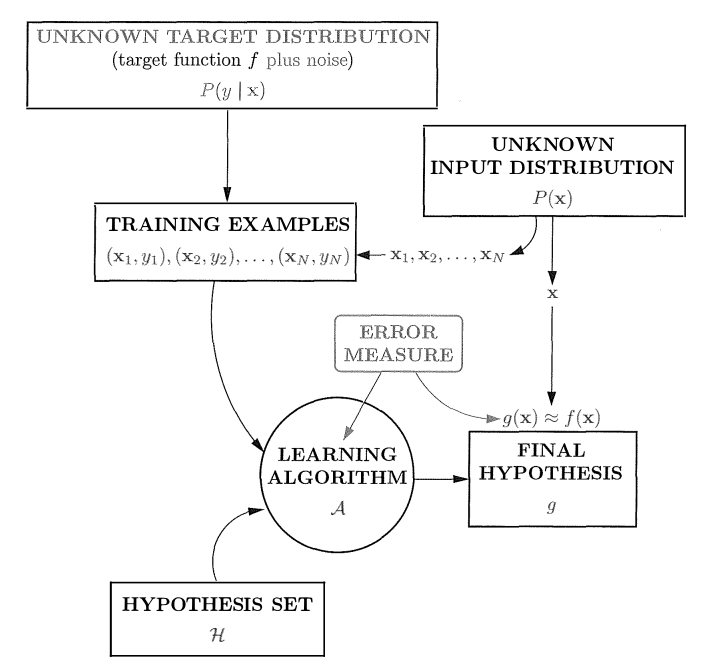
\includegraphics[scale=0.6]{img/Esquema AASupervisado.png}
        \caption{Esquema del problema de Aprendizaje Supervisado. Imagen extraída de \cite{data}}
        \label{fig:EsquemaAASupervisado}
    \end{figure}
    
%%%%%%%%%%%%%%%%%%%%%%%%%%%%%%%%%%%%%%%%%%%%%%%%%%%%%%%%%%%%%%%%%%%%%
%%%%%%%%%%%%%%%%%%%%%%%%%%%%%%%%%%%%%%%%%%%%%%%%%%%%%%%%%%%%%%%%%%%%%
%%%%%%%%%%%%%%%%%%%%%%%%%%%%%%%%%%%%%%%%%%%%%%%%%%%%%%%%%%%%%%%%%%%%%

\section{Paradigma ERM}


    
        
        Como se mencionó anteriormente, $\A$ recibe como entrada un conjunto de entrenamiento $S$, muestreado de manera $i.i.d.$ de $Z$ y debe proporcionar un predictor $h_S:\X \to \Y$. El objetivo es encontrar dicha hipótesis $h_S$ que minimice el error respecto de la distribución $P$ y $P(y|x)$. Tanto $P$ como $P(y|x)$ son desconocidas, el algoritmo no va a tener acceso al error de generalización (también conocido como error fuera de la muestra o error verdadero) definido en \eqref{eq:general_loss_function}, esto motiva la siguiente definición, la cual se conoce como error de entrenamiento, error empírico o error dentro de la muestra.
    
        
            \begin{definicion}[Error empírico - clasificación binaria]
                Dada $h\in \mathcal{H}$, $\ell$ una función de error y  ${S=\{(x_1,y_1),...,(x_m,y_m)\}}$ un conjunto de entrenamiento, se define el error empírico como 
                \begin{equation}
                \Rh_{S}(h) := \frac{1}{m} \sum_{i=1}^m [\mathbb{1}_{h(x_i) \not= y_i}]
                \end{equation}
                \noindent Cuando no haya lugar a dudas sobre el conjunto de entrenamiento, notaremos $\hat{R}(h)$ en vez de $\hat{R}_S(h)$
            \end{definicion}
            
            
        \begin{proposicion}\label{prop:esperanza del error empirico}
            Dada $h \in \mathcal{H}$ y un  conjunto de entrenamiento S extraído de manera $i.i.d$, entonces
            
            \begin{equation}
                \E[\hat{R}(h)] = R(h)
            \end{equation}
            \end{proposicion}
            
            \begin{proof}
            Usando la linealidad de la esperanza y la hipótesis, tenemos que 
            \begin{equation}
                \begin{aligned}
                    \E_{S \sim P^m} [\hat{R}(h)] & = \frac{1}{m}\sum_{i=1}^m \E_{S \sim P^m}[1_{h(x_i)\neq y_i}]  \\
                     & = \E_{x \sim P}[1_{h(x)\neq y}]  \\
                     & = R(h)
                \end{aligned}
            \end{equation}
            \end{proof}
        
        El error de generalización, desgraciadamente no vamos a poder calcularlo. Pero gracias al conjunto de entrenamiento tenemos una representación del mundo exterior disponible para ser usada por el algoritmo. Además, gracias a la proposición anterior, tenemos que bajo ciertos supuestos, la esperanza del error empírico es el error de generalización. Nuestros objetivo ahora es conseguir cumplir: 
        
        \begin{equation}\label{eq:objetivos_aprendizaje}
            \begin{aligned}
                \hat{R}(h) \approx 0 ,&&    \hat{R}(h) \approx R(h)
            \end{aligned}
        \end{equation}
        
        \noindent De este modo, al ser muy pequeño el error empírico y al estar muy próximo al error de generalización, vamos a lograr que el erro de generalización esté también próximo a cero, que sería lo ideal. \\
        
        
        El primer objetivo lo logramos buscando una hipótesis que minimice el error empírico, a este paradigma se le conoce como ERM, del inglés, \textit{Empirical Risk Minimization}. Más formalmente se busca una hipótesis $h_S \in \mathcal{H}$ tal que 
        \begin{equation}
           h_S \in argmin_{h \in \mathcal{H}} \hat{R}_S(h)
        \end{equation}
        donde $argmin$ denota el conjunto de hipótesis de $\mathcal{H}$ para las que se alcanza un mínimo sobre $\hat{R}_S(h)$ \\
        
        Con este paradigma vamos a tener que hacer frente a un gran inconveniente, que es la aparición de sobreaprendizaje, del cual hablaremos más adelante. Solo diremos que el sobreaprendizaje ocurre cuando encontramos una hipótesis $h^* \in \mathcal{H}$ de tal manera que $\Hat{R}(h^*)$ sea un valor muy pequeño y $R(h^*)$ un valor muy grande, es decir, $\hat{R}(h^*) \not\approx R(h^*)$, faltando de este modo al cumplimiento del primer objetivo en \eqref{eq:objetivos_aprendizaje} \\
        
        Para lidiar con esto, se puede restringuir la clase de hipótesis, lo que sesga hacia un conjunto particular de clasificadores. Este método es lo que se conoce como \textit{sesgo inductivo}, con esto se logra cumplir el segundo objetivo ($\Rh \approx R$) en detrimento del primero ($\Rh \approx 0$), ya que al restringir la clase de hipótesis puede ocurrir que no incluyamos las hipótesis para las que se alcance un mínimo. \\
        
        
        
        Con motivo de simplificar las cosas, particularizaremos al caso de clasificación binaria, es decir, cuando $\Y = \{0,1\}$. También se considerará el concepto de función objetivo, $f$, en vez de distribución objetivo, $P(y|x)$, aunque en verdad se puede considerar cualquiera. Vamos a definir los errores para este caso,

    
            \begin{definicion}[Error 0-1]
            Dado $h \in \mathcal{H}$, una función objetivo $f$, se define el error $0-1$ para todo ${z = (x,f(x))}$ como
            \begin{equation}
                \ell_{0-1}(h,z) = 
                \left\{
                \begin{array}{cc}
                     0 & h(x) = y \\
                     1 & h(x) \neq y
                \end{array}
                \right.
             \end{equation}
            \end{definicion}
        
        
            \begin{definicion}[Error de Generalización, Clasificación Binaria]\label{def:errorGeneralizacion}
            Dada una hipótesis $h \in \mathcal{H}$, una función objetivo $f$ y una distribución de probabilidad subyacente $P$ definimos el error de generalización de $h$ como
            \begin{equation}
                R_{P,f}(h) := \Pb_{x \sim P}[h(x) \neq f(x)] = P(\{x: h(x) \neq f(x)\}) \quad \forall x \in \X
            \end{equation}
            \noindent Los subíndices $P,f$ hacen énfasis en la distribución subyacente y en la función objetivo, pero cuando no quepa lugar a duda lo notaremos como $R(h)$ omitiendo los subíndices. \\
            \end{definicion}
        
\section{Aprendizaje PAC}

    A la hora de diseñar y analizar algoritmos que aprenden de los ejemplos se pueden plantear una serie de cuestiones tales como ¿Cuántos ejemplos son necesarios para aprender con éxito? ¿Existe un modelo general de aprendizaje? En esta sección vamos a formalizar y a tratar estas cuestiones introduciendo el marco de aprendizaje correcto probablemente aproximado (PAC). Dicho marco nos ayudará a definir la clase de funciones aprendibles en términos del número de puntos de la muestra necesarios para lograr una solución aproximada. \\
    
    Vamos a especificar cuándo una clase de hipótesis es PAC aprendible, para ello vamos a considerar una función objetivo $f$, en vez de una distribución objetivo $P(x,y)$, también consideraremos el caso de clasificación binaria aunque al final generalizaremos para cualquier función de pérdida. Vamos a suponer también lo que se conoce como hipótesis o asunción de realizabilidad. \\
    
    
    \begin{definicion}[Asunción de realizabilidad]
    La hipótesis o asunción de realizabilidad se basa en suponer que existe $h^* \in \mathcal{H}$ tal que $R_{P,f}(h^*) = 0$. 
    \end{definicion}
    
    \begin{observacion}
    Notamos que esta asunción implica con probabilidad 1 sobre una muestra aleatoria, $S$, donde las instancias son muestreadas acorde a $P$ y etiquetadas por $f$, que para cada hipótesis $h_S \in \Hc$ elegida acorde al criterio ERM, $\hat{R}_S(h_S) = 0$. Por lo que en este caso estamos más interesados en el error de generación que en el error empírico. \\
    \end{observacion}
    
    Como $R_{P,f}(h_S)$ depende del conjunto de entrenamiento y este se elige de manera aleatoria, tenemos una aleatoriedad implícita en la elección de $h_S$ y en consecuencia, en el error $R_{P,f}(h_S)$. No es cierto pensar que el conjunto $S$ baste para guiar la elección del algoritmo a una buena hipótesis ya que siempre existe una probabilidad de que los datos de entrenamiento que se han extraído sean muy pocos representativos de la distribución $P$. De aquí en adelante denotaremos a la probabilidad de elegir una muestra no representativa por $\delta$ y llamaremos $(1-\delta)$ el \textit{parámetro de confianza} de nuestra predicción. Además, como no podemos garantizar una predicción perfecta de las etiquetas, introducimos otro parámetro para la calidad de la predicción y lo llamaremos \textit{parámetro de precisión} denotado como $\epsilon$. Interpretaremos $R_{P,f}(h_S) > \e$ de manera negativa, viéndolo como un fallo o fracaso en elección de la hipótesis, por rebasar el umbral de precisión (en la proposición \ref{pro:cp_negativo} daremos una cota superior para la probabilidad de que ocurra este suceso), mientras que $R_{P,f}(h_S) \leq \e$ lo veremos como una predicción aproximadamente correcta. \\
    
    
    
        \begin{definicion}[Aprendizaje PAC]
        Una clase de hipótesis $\mathcal{H}$ es PAC aprendible cuando exista una función $m_{\mathcal{H}}:(0,1)^2 \to \N$ y un algoritmo de aprendizaje $\mathcal{A}$ con la siguiente propiedad: Para todo $\e, \delta \in (0,1)$, para cada distribución $P$ sobre $\X$ y para cada función objetivo $f:\X \to \{0,1\}$, si se cumple la hipótesis de realizabilidad con respecto $\Hc, P,f$, entonces cuando ejecutamos el algoritmo de aprendizaje $\A$ en $m\geq m_{\Hc}(\e,\de)$ $i.i.d.$ ejemplos generados por $P$ y etiquetados por $f$, $\A$ devuelve una hipótesis $h \in \Hc$ tal que,
            \begin{equation}
                \Pb_{S\sim P^m}[R_{P,f}(h) \leq \e] \geq 1 - \de
            \end{equation}
            
        \end{definicion}
        
    En esta definición, la \textit{precisión}, $\e$, determina como de lejos está el clasificador del óptimo y corresponde a la parte \textit{AC} de \textit{PAC}, del inglés, \textit{approximately correct}. El parámetro de confianza, $(1-\de)$ indica cómo de probable es que el clasificador cumpla ese requisito la precisión, y corresponde a la parte de \textit{probability} del \textit{PAC}. \\
    
    La función $m_{\mathcal{H}}:(0,1)^2 \to \N$ determina la complejidad de la muestra para aprender $\Hc$, esto es, cuantos ejemplos se requieren para garantizar una solución PAC. La complejidad de la muestra depende e la precisión ($\e$) y de la confianza ($\de$), pero también depende de algunas propiedades de la clase de hipótesis $\Hc$ que veremos más adelante. \\
    


    \begin{proposicion}\label{pro:cp_negativo}
        Sea $f$ una función de etiquetado, $S_{|x} = \{(x_1,...,x_m\}$ un conjunto de entrenamiento y $P$ una distribución de probabilidad subyacente sobre la que se han extraído las muestras de manera $(i.i.d.)$. Suponemos también que el conjunto de hipótesis $\mathcal{H}$ es finito y que se cumple la hipótesis de realizabilidad, entonces
        
        \begin{equation}
            P^m(\{S_{|x} : R_{P,f}(h_S) > \e\}) \leq |\mathcal{H}| e^{-\e m}
        \end{equation}
    \end{proposicion}
    
    \begin{proof}
     Consideramos el conjunto de hipótesis incorrectas
         
         \begin{equation}
             \Hc_B = \{ h \in \Hc : R_{P,f} > \e\}
         \end{equation}
    
    \noindent y el conjunto de de las muestras de entrenamiento para las que existe un hipótesis incorrecta que hacen al error empírico cero. 
    
        \begin{equation}
            M = \{ S_{|x} : \exists h \in \Hc_B , \hat{R}_S(h) = 0 \}
        \end{equation}
 
    Podemos ver el conjunto $M$ como aquel en el que las hipótesis parecen buenas sin serlo. El objetivo es acotar la probabilidad del suceso $R_{P,f}(h_S) > \e$. Por la hipótesis de realizabilidad se sigue que el suceso $R_{P,f}(h_S) > \e$ ocurre solo si existe $h\in \Hc_B$ con $\hat{R}_S(h) = 0$, por lo que
    \begin{equation}
        \{S_{|x}: R_{P,f}(h_S) > \e \} \subseteq M
    \end{equation}
    
    \noindent Reescribiendo M como $M = \bigcup_{h \in \Hc_B}\{ S_{|x}: \hat{R}_S(h) = 0\}$, tenemos que     
    \begin{equation}
        \begin{aligned}
            P^m(\{ S_{|x}:R_{P,f}(h_S) > \e \}) & \leq  P^m\Big(\bigcup_{h \in \Hc_B} \{ S_{|x}:\hat{R}_S(h) = 0 \} \Big) \\
            & \leq \sum_{h \in \Hc_B} P^m(\{ S_{|x}:\hat{R}_S(h) = 0 \} ) \\
            & = \sum_{h \in \Hc_B} P^m(\{ S_{|x}: h(x_i) = f(x_i) \; \forall i \} ) \\
            & = |\Hc_B| (1 - R_{P,f}(h))^m  \\
            & \leq  |\Hc| (1 - \e)^m  \\
        \end{aligned}
    \end{equation}

    \noindent Usando que $1 - e \leq e^{-\e}$ se sigue que $|\Hc| (1 - \e)^m  \leq |\Hc|e^{-m \e}$
    
    \end{proof}

    
    \begin{corolario}
    Bajo la asunción de realizabilidad, toda clase de hipótesis finita es PAC aprendible verificando, 
    
    \begin{equation}
        m_{\Hc} (\e, \de) \leq \lceil \frac{log(|\Hc|/\de)}{\e} \rceil
    \end{equation}
    
    \end{corolario}
    
    \begin{observacion}
    Notamos que el error de generalización se aproxima a cero cuando el tamaño del conjunto de entrenamiento aumenta.
    \end{observacion}
    
    
    
    
%%%%%%%%%%%%%%%%%%%%%%%%%%%%%%%%%%%%%%%%%%%%%%%%%%%%%%%%%%%%%%%%%%%%%
%%%%%%%%%%%%%%%%%%%%%%%%%%%%%%%%%%%%%%%%%%%%%%%%%%%%%%%%%%%%%%%%%%%%%
%%%%%%%%%%%%%%%%%%%%%%%%%%%%%%%%%%%%%%%%%%%%%%%%%%%%%%%%%%%%%%%%%%%%%    
    
    
    \subsection{Agnostic PAC}
        La definición de PAC que hemos dado no es para nada general, ya que parte de la premisa de realizabilidad, que es una hipótesis bastante fuerte la cual no se cumple en la mayoría de los casos. Motivo por el cual vamos a generalizarla para abarcar un mayor número de casos. Para ello relajamos las hipótesis eliminando la asunción de realizabilidad y suponiendo una distribución objetivo conjunta $P(x,y)$ en vez de una función objetivo, $f$.\\
    
        \begin{definicion}[Agnostic-PAC]
         Una clase de hipótesis $\Hc$ es PAC agnóstica aprendible si existe una función $m_{\Hc}:(0,1)^2 \to \N$ y un algoritmo de aprendizaje $\A$ con la siguiente propiedad: Para todo $\e, \de \in (0,1)$ y para todo distribución $P$ conjunta sobre $\X \times 
         \{0,1\}$, cuando ejecutemos el algoritmo de aprendizaje sobre $m \geq m_{H}$ ejemplos $i.i.d.$ generados por la distribución conjunta $P$, el algoritmo devuelve una hipótesis $h \in \Hc$ tal que 
         
         \begin{equation}
             \Pb_{S \sim P^m}[R_P(h) - min_{h' \in \Hc}R_P(h') \leq \e] \geq 1 - \de
         \end{equation}
                
         \end{definicion}
                
        
        Rizando aún más el rizo en pos de lograr una mayor generalización, notamos que la definición anterior solo abarca el caso de clasificación binaria, es decir, los supuestos en los cuales $\Y = \{0,1\}$ y $\ell = \ell_{0-1}$ y la función de error de generalización viene dada por \ref{def:errorGeneralizacion}. 
        
        \begin{definicion}[Agnostic-PAC  para una función de pérdida general]
        Una clase de hipótesis $\Hc$ es PAC-Agnóstica con respecto a un conjunto $Z \subset \X \times \Y$ y una función de pérdida medible $\ell: \Hc \times Z \to \R^+$ cuando exista una función $m_{\Hc}:(0,1)^2 \to \N$ y un algoritmo de aprendizaje $\A$ cumpliendo la siguiente propiedad: Para cada $\e ,\de \in (0,1)$ y para cada distribución $P$ sobre $Z$, cuando ejecutamos el algoritmo de aprendizaje sobre  $m \geq m_{\Hc}(\e, \de)$ ejemplos $i.i.d.$ generados por $P$, el algoritmo devuelve $h \in \Hc$ tal que,
        
        \begin{equation}
            \Pb_{S\sim P}[L_P(h) - min_{h' \in \Hc} L_P(h') \leq \e] \geq 1 - \de
        \end{equation}
        
        donde $L_D(h) = \E_{z\sim P}[\ell(h,z)]$ 
        
        \end{definicion}
    


%%%%%%%%%%%%%%%%%%%%%%%%%%%%%%%%%%%%%%%%%%%%%%%%%%%%%%%%%%%%%%%%%%%%%
%%%%%%%%%%%%%%%%%%%%%%%%%%%%%%%%%%%%%%%%%%%%%%%%%%%%%%%%%%%%%%%%%%%%%
%%%%%%%%%%%%%%%%%%%%%%%%%%%%%%%%%%%%%%%%%%%%%%%%%%%%%%%%%%%%%%%%%%%%%
\subsection{Aprendizaje por Convergencia Uniforme}

    En la sección anterior, vimos que una clase de hipótesis finita es PAC aprendible suponiendo la hipótesis de realizabilidad. En esta sección vamos eliminar dicha asunción para demostrar que cualquier clase de hipótesis finita es Agnostic-PAC aprendible. Para ello vamos a aplicar el concepto de convergencia uniforme en el sentido de que vamos a necesitar que uniformemente sobre todas las hipótesis de la clase de hipótesis, el riesgo empírico esté próximo al riesgo verdadero. \\
    
    
    \begin{definicion}[muestra $\e$-representativa]
    Se dice que un conjunto de entrenamiento es $\e$-representativo con respecto a un dominio $Z$, una clase de hipótesis $\Hc$, una función de pérdida $\ell$ y una distribución subyacente $P$ cuando,
    \begin{equation}
        |\hat{R}_{S}(h) - R_{P,f}(h)| \leq \e \quad \forall h \in \Hc
    \end{equation}
    \end{definicion}

    
    \begin{lema}\label{lema:UC}
    Sea $S$ un conjunto de entrenamiento $\frac{\e}{2}$-representativo con respecto a $Z, \Hc, \ell$ y $P$. Entonces, cualquier hipótesis $h_S \in argmin_{h \in \Hc}L_S(h)$ satisface que,
    \begin{equation}
        R_{P,f}(h_S) \leq min_{h \in \Hc} R_{P,f}(h) + \e
    \end{equation}
    \end{lema}
    
    El lema anterior viene a decir que para cualquier muestra que sea $\e/2$-representativa el criterio ERM garantiza una buena hipótesis de salida. La demostración es prácticamente inmediata, para ello basta considerar $h\in \Hc$ arbitraria, entonces
    
    \begin{equation}
        R_{D,f}(h_S) \leq \Rh_S(h_S) + \frac{\e}{2} \leq \Rh_S(h) + \frac{\e}{2} \leq R_{P,f}(h) + \frac{\e}{2} + \frac{\e}{2} = R_{P,f}(h) + \e
    \end{equation}
    
    \noindent al ser $h$ una hipótesis arbitraria, tenemos que lo anterior se cumple para todo $h \in \Hc$. 
    
    
    
    
    \begin{definicion}[Convergencia uniforme]\label{def:UC}
       Decimos que una clase de hipótesis $\Hc$ cumple la propiedad de la convergencia uniforme (con respecto a un dominio $Z$ y una función de error $\ell$) cuando exista una función $m_{\Hc}^{UC}:(0,1)^2 \to \N$ tal que para cada $\e, \de \in (0,1)$ y para cada distribución de probabilidad, $P$, sobre $Z$, si el conjunto de entrenamiento, $S$, tiene $m\geq m_{\Hc}^{UC}(\e,\de)$ ejemplos tomados de manra $(i.i.d.)$ de acuerdo a $P$, entonces con probabilidad al menos $1-\de$ el conjunto de entrenamiento $S$ es $\e$-representativo.
    \end{definicion}
    
    Análogo a la definición de PAC, la función $m_{\Hc}^{UC}$ mide la complejidad de la muestra mínima, esto es, el número mínimo de ejemplos que necesitamos para asegurar con probabilidad al menos $1 - \de$ que la muestra es $\e$-representativa. El término \textit{uniforme} hace referencia a tener un tamaño de muestra fijo que funcione para todas las hipótesis de $\Hc$ y sobre todas las posibles distribuciones de probabilidad sobre el dominio. Aplicando el lema \ref{lema:UC} y la definición \ref{def:UC} obtenemos el siguiente corolario. \\
    
    \begin{corolario}\label{corolario:APAC-UC}
       Si una clase de hipótesis cumple la propiedad de convergencia uniforme. La clase de funciones es Agnostic-PAC aprendible con una complejidad de la muestra ${m_{H}(\e,\de) \leq m_{\Hc}^{UC}(\frac{\e}{2},\de)}$. Además, el paradigma $ERM_{\Hc}$ es un criterio de aprendizaje exitoso para $\Hc$. 
    \end{corolario}
   
   
   \begin{observacion}
   En vista del colorario anterior, la afirmación de que toda clase de hipótesis finita es Agnostic-PAC aprendible se producirá una vez se estableza que la convergencia uniforme se mantiene para clases de hipótesis finita. \\
   \end{observacion}
   
   
   \begin{proposicion}
   Sea $\Hc$ un conjunto de hipótesis finito, sea $Z$ un dominio y sea ${\ell:\Hc \times Z \to [0,1]}$ una función de error. Entonces, $\Hc$ cumple la propiedad de convergencia uniforme con una complejidad de la muestra,
   \begin{equation}
       m_{\Hc}^{UC}(\e,\de) \leq \lceil \frac{\log(2|\Hc|/\de)}{2\e^2} \rceil
   \end{equation}
   
   Además, $\Hc$ es Agnostic-PAC aprendible aplicando el criterio ERM y la complejidad de la muestra verifica,
   \begin{equation}
        m_{\Hc}(\e,\de) \leq  m_{\Hc}^{UC}(\e,\de) \leq \lceil \frac{\log(2|\Hc|/\de)}{2\e^2} \rceil
   \end{equation}
   \end{proposicion}

    \begin{proof}
    
    Fijamos $\e,\de$ y debemos encontrar un tamaño ,$m$, para una muestra, $S = (z_1,...,z_m)$, extraída de manera $i.i.d.$ de $P$ que verifique, con probabilidad al menos $1-\de$ que para todo $h \in \Hc$, $|\Rh_S(h) - R_{P}(h) | \leq \e$. Esto es,
        \begin{equation}
            P^m(\{ S: \forall h \in \Hc, | \Rh_S(h) - R_P(h) | \leq  \e \}) \geq 1 - \de
        \end{equation}
    \noindent y probar lo anterior equivale a probar que,
        \begin{equation}
            P^m(\{ S: \exists h \in \Hc, |\Rh_S(h) - R_P(h) | >  \e \}) \geq \de
        \end{equation}
    
    \noindent Escribiendo, 
        \begin{equation}
           \{ S: \exists h \in \Hc, |\Rh_S(h) - R_P(h) | >  \e \}) = \bigcup_{h\in\Hc} \{S: |\Rh_S(h) - R_P(h) | >  \e\}
        \end{equation}
        
    \noindent tenemos que,
        \begin{equation}\label{eq:aux01}
            P^m(\{ S: \exists h \in \Hc, |\Rh_S(h) - R_P(h) | >  \e \}) \leq \sum_{h \in \Hc} P^m(\{S: |\Rh_S(h) - R_P(h) | >  \e\})
        \end{equation}
    
    Recordemos que la definición general de los errores era, $R_P(h) = \E_{z\sim P}[\ell(h,z)]$ y $\Rh(h) = \frac{1}{m} \sum_{i=1}^m \ell(h,z_i)$. Como cada $z_i$ es muestreado de manera $i.i.d.$ de P, el valor esperado de la variable aleatoria $\ell(h,z_i)$ es $R_P(h)$. Además por la proposición \ref{prop:esperanza del error empirico} se sigue que $|R_{D}(h) - \Rh_S(h)|$ es la desviación de la variable aleatoria $\Rh_S(h)$ con respecto a su esperanza. Por lo que debemos de demostrar que los valores de $\Rh_S(h)$ se concentran en torno a su valor esperado. \\
    
    Fijamos $h \in \Hc$ y consideramos las variables aleatorias $\ell_i = \ell(h,z_i)$ para todo $i=1,...,m$. Como $(z_1,...,z_m)$ es una muestra de variables aleatorias $i.i.d.$, se sigue que $(\ell_1,...,\ell_m)$ también lo es. Vamos a asumir que el rango de $\ell(h,z_i) \in [0,1]$ para todo $i=\{1,...,m\}$. Denotamos $R_P(h) = \mu$ y aplicando la \textit{desigualdad de Hoeffding} \eqref{eq:Hoeffding} llegamos a que,
    
        \begin{equation} \label{eq:Hoeffding_error}
            P^m(\{S: |\Rh_S(h) - R_D(h)| > \e\}) = \Pb \Big[ \Big| \frac{1}{m} \sum_{i=1}^m \ell_i - \mu \Big| > \e \Big] \leq 2 \exp{(-2m\e^2)}
        \end{equation}
    \noindent y aplicando \eqref{eq:aux01} se sigue que,
        \begin{equation}
            P^m(\{ S: \exists h \in \Hc, |\Rh_S(h) - R_D(h)| > \e \}) \leq \sum_{h\in \Hc} 2 e^{-2m\e^2} = 2 |\Hc| e^{-2m\e^2}
        \end{equation}
    \noindent Eligiendo ahora,
        \begin{equation}
            m \geq \frac{\log(2 |\Hc|/\de)}{2\e^2}
        \end{equation}
    \noindent conseguimos
        \begin{equation}
             P^m(\{ S: \exists h \in \Hc, |\Rh_S(h) - R_P(h) | >  \e \}) \geq \de
        \end{equation}
        
        
    \noindent La segunda parte es inmediata del corolario \ref{corolario:APAC-UC}
    \end{proof}


%%%%%%%%%%%%%%%%%%%%%%%%%%%%%%%%%%%%%%%%%%%%%%%%%%%%%%%%%%%%%%%%%%%%%
%%%%%%%%%%%%%%%%%%%%%%%%%%%%%%%%%%%%%%%%%%%%%%%%%%%%%%%%%%%%%%%%%%%%%
%%%%%%%%%%%%%%%%%%%%%%%%%%%%%%%%%%%%%%%%%%%%%%%%%%%%%%%%%%%%%%%%%%%%%

\subsection{Cotas de Generalización para clases de hipótesis finitas}

Anteriormente se comentó que uno de los objetivos a los que aspiramos es a conseguir una hipótesis $g\in \Hc$ que se aproxime todo lo posible a la función o distribución objetivo. Para ello usamos una muestra $S$ extraída de manera $i.i.d.$ de acuerdo $P$ e intentamos minimizar el funcional $\Rh_S$. Sin embargo, puede ocurrir que $\Rh(g) \approx 0$ pero $\Rh_S \not\approx R_P$, lo cual indica que la hipótesis elegida no generaliza bien. Vamos a medir el grado de generalización dada una hipótesis $g \in \Hc$ como $|\Rh_S(g) - R_P(g)|$ y en esta sección daremos una serie de cotas de generalización. \\
    
    
    La desigualdad de Hoeffding nos da una manera de acotar el error de generalización en términos probabilísticos,
    
    \begin{equation}
        \Pb \Big[ \Big| \Rh_S(g) - R_{P}(g) \Big| \geq \e \Big] \leq 2 e^{-2m\e^2 }
    \end{equation}
    
    \noindent para cualquier $\e > 0$. Lo cual es equivalente a decir que con probabilidad al menos $1 - 2 e^{-2m\e^2 }$, ocurre que $|R_{P}(g) - \Rh_S(g)| \leq \e$, lo que implica que $R_{P}(g) \leq \Rh_S(g) + \e$, e identificando $\de = 2e^{-2m\e^2}$ y despejando $\e$ llegamos a que con probabilidad al menos $1 - \de$,
    
    \begin{equation}\label{eq:Generalization Bound}
        R_{P}(g) \leq \Rh_S(g) + \sqrt{\frac{1}{2m} \log{\frac{2}{\de}}}
    \end{equation}
    
    \noindent a esta desigualdad la llamamos cota de generalización porque acota $R_{P}$ en términos de $\Rh_S$. Por otro lado, la desigualdad  $|R_{P}(g) - \Rh_S(g)| \leq \e$, implica también que $R_{P}(g) \geq \Rh_S(g) - \e$. Esto importante tenerlo en cuenta, pero de manera más sutil. No solo queremos que la hipótesis $g$ que escojamos (la que minimize el error empírico) siga funcionando bien fuera de la muestra, sino que también queremos asegurarnos de que lo hicimos lo mejor que pudimos con la elección de la hipótesis en $\Hc$. La cota $R_{P}(g) \geq \Rh_S(g) - \e$, nos asegura que no podríamos hacerlo mejor, ya que para cada hipótesis $h$ con mayor riesgo empírico que $g$, $\Rh_S(g) \leq \Rh_S(h)$, tendremos $R_P(g) \geq R_P(h)$. \\
    
    Enunciemos lo anteriormente comentado,
    
    \begin{proposicion}
     Sea $\e >0$ fijo, y sea $S$ una muestra $i.i.d.$ de tamaño $m$. Entonces, para cualquier hipótesis $g:\X \to \{0,1\}$ se cumple que,
     \begin{equation}
         \begin{aligned}
              \Pb_{S \sim P^m}[ \Rh(h) - R_P(g) \geq \e ] & \leq e^{-2m\e^2} \\
              \Pb_{S \sim P^m}[ \Rh(h) - R_P(g) \leq -\e ] & \leq e^{-2m\e^2}
         \end{aligned}
     \end{equation}
     En particular,
     \begin{equation}
         \Pb_{S \sim P^m}[ |\Rh(g) - R_P(g) | \geq \e ]  \leq e^{-2m\e^2}
     \end{equation}
    \end{proposicion}
    
    \begin{proposicion}\label{prop:desfijadah}
     Fijamos $g:\X \to \{0,1\}$ una hipótesis. Sea $S$ una muestra $i.i.d.$ de tamaño $m$ Entonces para cualquier $\de>0$ la siguiente desigualdad se cumple con probabilidad al menos $1-\de$,
     \begin{equation}
         R_P(g) \leq \Rh_S(g) + \sqrt{\frac{1}{2m}\log{\frac{2}{\de}}}
     \end{equation}
    \end{proposicion}
    
    
    Notamos que la cota dada por la desigualdad de la proposición \ref{prop:desfijadah} solo es válida cuando fijamos previamente una hipótesis $g \in \Hc$. Podemos preguntarnos a continuación por la existencia de otra cota en términos del conjunto de hipótesis $\Hc$ siempre que sea finito. Esta pregunta motiva lo que sigue.
    
    
    \begin{proposicion}[Caso: $\Hc$ finito y consistente]
         Sea $\Hc$ una clase de hipótesis finita. Sea una función objetivo $f$, y se $S$ una muestra de tamaño $m$ extraída de manera $i.i.d.$ de acuerdo a una distribución de probabilidad $P$. Si asumimos la hipótesis de realizabilidad entonces tenemos que para cualquier $\e,\de > 0$, con probabilidad al menos $1-\de$,
         \begin{equation}
            R_P(h_S) \leq \frac{1}{m}\Big( \log\Big(\frac{|H|}{\de}\Big) \Big) 
         \end{equation}
    \end{proposicion}
    
        \begin{proof}
        Por la proposición \ref{pro:cp_negativo} tenemos que
            \begin{equation}
                \Pb[R_{P}(h_S) > \e] \leq |\Hc| e^{-em} = 1 - \de
            \end{equation}
        \noindent luego, 
            \begin{equation}
                \Pb[R_{P}(h_S) \leq \e] \geq  |\Hc| e^{-em} 
            \end{equation}
        \noindent tomando $\de = |\Hc| e^{-em}$, implica que $\e = \frac{1}{m}\log\Big( \frac{|H|}{\de} \Big)$, por lo que,
            \begin{equation}
                R_P(h_S) \leq \frac{1}{m}\log\Big( \frac{|H|}{\de} \Big)
            \end{equation}
        \end{proof}


    \begin{proposicion}[Caso: $\Hc$ finito y no consistente]

    Sea $\Hc$ un conjunto de hipótesis finito, $S$ un conjunto de entrenamiento de tamaño $m$ muestreado de manera $i.i.d.$. Entonces, para cualquier $\de$ con probabilidad al menos $1-\de$,
    \begin{equation}
    \forall h \in \Hc, \quad R(h) \leq \Rh(h) + \sqrt{\frac{1}{2m} \log \Big( \frac{2|\Hc|}{\de} \Big)}
    \end{equation}
    \end{proposicion}


    \begin{proof}
    Sean $h_1,...,h_{|\Hc|}$ las hipótesis de $\Hc$ y teniendo en cuenta la proposición \ref{prop:desfijadah},
    
    \begin{equation}
        \begin{aligned}
            \Pb[\exists h \in \Hc : |\Rh(h) - R(h)| > \e] & = \Pb \Big[\bigcup_{i = {1}}^{|\Hc|} |\Rh(h_i) - R(h_i) | > \e\Big] \\
            & \leq \sum_{i = 0}^{|\Hc|} \Pb[|\Rh(h_i) - R(h_i)| > \e] \\
            & \leq 2 |\Hc| \exp{(-2m\e^2)}
        \end{aligned}
    \end{equation}
    
    Reproduciendo el razonamiento que hicimos para obtener la ecuación \eqref{eq:Generalization Bound}, se concluye la prueba.
    \end{proof}

%%%%%%%%%%%%%%%%%%%%%%%%%%%%%%%%%%%%%%%%%%%%%%%%%%%%%%%%%%%%%%%%%%%%%
%%%%%%%%%%%%%%%%%%%%%%%%%%%%%%%%%%%%%%%%%%%%%%%%%%%%%%%%%%%%%%%%%%%%%
%%%%%%%%%%%%%%%%%%%%%%%%%%%%%%%%%%%%%%%%%%%%%%%%%%%%%%%%%%%%%%%%%%%%%
    
\section{La dimensión de Vapnik-Chervonenkis}

    Hemos visto que la finitud de la clase de hipótesis es una condición suficiente pero no necesaria para un correcto aprendizaje. En esta sección daremos una caracterización y para ello introduciremos nuevos conceptos tales como la función de crecimiento y la dimensión VC. Nos seguiremos centrando en el caso de clasificación binaria. \\
    
    Vamos a comenzar enunciando un importante teorema en su versión para clasificación binaria que nos dice que no existe un algoritmo universal que sea exitoso para todas las tareas de aprendizaje. 
    
    \begin{teorema}[No-Free-Lunch]
    Sea $\A$ cualquier algoritmo de aprendizaje para una tarea de clasificación binaria, una función de error $\ell_{0-1}$, un dominio $\X$. Sea $m < |\X|/2$ el tamaño del conjunto de entrenamiento. Entonces existe una distribución $P$ sobre $\X\times\{0,1\}$ tal que,
    \begin{enumerate}
        \item Existe una función $f:\X \to \{0,1\}$ con $R_{P}(f) = 0$
        \item Con probabilidad al menos $\frac{1}{7}$ sobre la elección de $S\sim P^m$ tenemos que $R_{P}(\A(S)) \geq \frac{1}{8}$
    \end{enumerate}
    \end{teorema}
    
    La demostración la encontramos en $\cite{UML}$. Este teorema nos dice que para cada algoritmo de aprendizaje, existe una tarea en la que falla, incluyo cuando esta puede ser aprendida satisfactoriamente por otro algoritmo. Por tanto, si usamos un predictor ERM sobre una clase de hipótesis de todas las funciones $h:\X \to \{0,1\}$, en virtud del teorema No-Free-Lunch tenemos que cualquier algoritmo que elija su salida entre las hipótesis de $\Hc$ y en particular el predictor ERM, fallará en alguna tarea de aprendizaje, por tanto, esta clase no es aprendible por PAC, formalizándolo quedaría como \\
    
    \begin{corolario}
    Sea X un dominio infinito y $\Hc$ el conjunto de todas las funciones de $X$ a $\{0,1\}$. Entonces, $\Hc$ no es PAC aprendible.
    \end{corolario}

\subsection{Desigualdad VC}
    
    La definición de la función de crecimiento se basa en el número de hipótesis distintas en $\Hc$, pero solo sobre un conjunto finito de puntos, $C = \{x_1,...x_n\} \subset \X$. Si $h \in \Hc$ se aplica sobre dicho conjunto, obtendremos una N-tupla, $(h(x_1),...,h(x_n))$ con valores pertenecientes a $\{0,1\}$, a la cual llamaremos dicotomía. Cada $h \in \Hc$ genera una dicotomía en $C$, y puede ocurrir que dos hipótesis distintas generen también la misma dicotomía, en cuyo caso, la función de crecimiento solo contabilizará una de ellas. \\
    
     \begin{definicion}[Dicotomías generadas por $\Hc$] 
     Las dicotomías generadas por $\Hc$ son los puntos definidos por 
     \begin{equation}
     \Hc(C) = \Hc(x_1,...,x_n) = \{(h(x_1),...,h(x_n) | h \in \Hc)\}
     \end{equation}
     \end{definicion}
     
     \begin{definicion}[función de crecimiento]
     Sea $\Hc$ una clase de hipótesis. La función de crecimiento de $\Hc$, $m_{\Hc}:\N \to \N$ se define como 
     \begin{equation}
     m_{\Hc}(N) = \underset{x_1,...,x_N \in \X}{max} |\Hc(x_1,...,x_N)|
     \end{equation}
     \end{definicion}
     
     En otras palabras, la función de crecimiento es el número máximo de dicotomías que podemos obtener de $\Hc$ usando $N$ puntos. Para calcular $m_{\Hc}$, consideramos todas los posibles elecciones de $N$ puntos de $\X$ y tomamos aquella elección que nos de el mayor número de dicotomías. Podemos interpretar $m_{\Hc}$ como una medida del número de hipótesis efectivas en $\Hc$ considerando $N$ puntos en vez del conjunto $\X$ completo. Además, como $\Hc(C) \subseteq \{0,1\}^N$ tenemos que,
     $$m_{\Hc}(N) \leq 2^N$$
     Si $\Hc$ es capaz de generar todas las posibles dicotomías en $C$, diremos que $\Hc$ explica o separa los elementos de $C$. \\
     
    \begin{definicion}[Punto de ruptura]
    Si ningún conjunto $C$ de tamaño $k$ no puede ser explicado por $\Hc$, entonces diremos que $k$ es un punto de ruptura para $\Hc$
    \end{definicion}
    
    
    \begin{definicion}[Dimensión Vapnik-Chervonenkis]\label{def:VC}
    La dimensión VC de una clase de hipótesis $\Hc$, denotada como $d_{VC}(\Hc)$ o simplemente $d_{VC}$ es el valor más grande de $N$ para el cual $m_{\Hc}(N) = 2^N$. Si $m_{\Hc}(N) = 2^N$ para todo $N$, entonces $d_{VC}(\Hc) = \infty$.
    \end{definicion}
    
    \begin{observacion}~\smallskip
    \begin{enumerate}
        \item Notamos que si $k$ es un punto de ruptura entonces, $m_{\Hc}(k) < 2^k$.
        \item Si $d_{VC} < \infty$ entonces $k = d_{VC} + 1$ es un punto de ruptura de $m_{\Hc}(N)$ y es el menor punto de ruptura.
    \end{enumerate}
    \end{observacion}
    
    
    Gracias a la introducción de la función de crecimiento y de la dimensión VC tenemos que aunque la clase de funciones sea infinita, la dimensión VC puede ser finita, lo que nos permitirá extender el concepto de PAC a clases de hipótesis infinitas. En cambio, puede ocurrir que la dimensión VC sea infinita y en este caso, tenemos como consecuencia casi inmediata del teorema No-Free-Lunch los siguiente corolarios. \\
    
    \begin{corolario} ~\smallskip
    \begin{enumerate}
    
    \item Sea $\Hc$ una clase de hipótesis tal que $d_{VC}(\Hc) = \infty$, entonces $\Hc$ no es PAC-aprendible.
    \item Sea $\X$ un dominio infinito y $\Hc$ el conjunto de todas las funciones que mapean $\X$ a $\{0,1\}$. Entonces, $\Hc$ no es PAC aprendible. 
   
    \end{enumerate}
    \end{corolario}
    
    Entonces nuestro objetivos se centrarán en estudiar qué es lo que ocurre cuando la dimensión VC es finita. Pero antes, vamos a ver un lema resaltando la importancia del mismo por permitirnos dar una cota polinómica para la función de crecimiento siempre y cuando la dimensión VC sea finita. Es más, se puede simplificar la cota del lema para enfatizar aún más la dependencia que existe con $d_{VC}$. \\ 
    
    \begin{lema}[Lema de Sauer-Shelah-Perles]\label{lema:Sauer}
    Sea $\Hc$ una clase de hipótesis con $d_{VC} < \infty$. Entonces, para todo $N$, 
    \begin{equation}
    m_{\Hc}(N) \leq \sum_{i=0}^{d_{VC}} \binom{N}{i}
    \end{equation}
    \noindent En particular, si $N > d_{VC} $, entonces,
    \begin{equation}
        m_{\Hc}(N) \leq \Big( \frac{e N }{d_{VC}} \Big)^{d_{VC}}
    \end{equation}
    \end{lema}
    
    La demostración consiste en realizar una inducción y en aplicar sencillas operaciones combinatorias por lo que la vamos a omitir (se puede encontrar en el capítulo 3 de \cite{FML}). \\
    

    \begin{corolario}\label{corolario:cotapolinomicaVC}
    Sea $\Hc$ una clase de hipótesis con $d_{VC} < \infty$, Entonces para todo N se cumple,
    \begin{equation}
        m_{\Hc}(N) \leq N^{d_{VC}} + 1
    \end{equation}
    \end{corolario}
    
    Basándonos en la definición y en el lema anterior, observamos que la función de crecimiento presenta dos casuísticas. Si ${d_{VC} = \infty}$ tenemos que por un lado ${m_{\Hc}(N) = 2^N}$ para todo ${N \in \N}$. En cambio, si $d_{VC} < \infty$ tenemos que ${m_{\Hc}(N) = 2^N}$ para ${N \leq d_{VC}}$ o bien ${m_{\Hc}(N) \leq N^{d_{VC}}+1}$ para ${N > d_{VC}}$. \\
    
    Damos cabida ahora al resultado más importante de esta sección, la desigualdad VC, la cual nos da una cota probabilística en función de la función de crecimiento de cuan alejados están el error empírico del real. \\
    
    \begin{teorema}[Desigualdad VC]\label{teorema:VCDes}
    Para todo $\e > 0$ se tiene,
    \begin{equation}
        \Pb[\underset{h \in \Hc}{sup} |\Rh(h) - R(h)| > \e] \leq 4 m_{\Hc}(2N)e^{-\frac{1}{8}\e^2N}
    \end{equation}
    \end{teorema}
    
    Esta desigualdad es válida para cualquier función objetivo o distribución objetivo y para cualquier distribución. La probabilidad es sobre conjuntos de tamaño $N$. Cada conjunto se genera $i.i.d.$ con cada puntos extraído de manera independiente de acuerdo a una distribución de probabilidad $P(x,y)$. \\
    
    


    
%%%%%%%%%%%%%%%%%%%%%%%%%%%%%%%%%%%%%%%%%%%%%%%%%%%%%%%%%%%%%%%%%%%%%
%%%%%%%%%%%%%%%%%%%%%%%%%%%%%%%%%%%%%%%%%%%%%%%%%%%%%%%%%%%%%%%%%%%%%
%%%%%%%%%%%%%%%%%%%%%%%%%%%%%%%%%%%%%%%%%%%%%%%%%%%%%%%%%%%%%%%%%%%%%
    
\subsection{Cota de Generalización VC}    

    Hasta ahora hemos tratado con clases de hipótesis finitas, que por el corolario \ref{corolario:APAC-UC} sabemos que son Agnostic-PAC, pero...¿Qué ocurre cuando la clase sea infinita? Para responder a esta cuestión nos adentramos en la dimensión Vapnik-Chervonenkis, en donde el papel fundamental ya no lo juega el cardinal de $\Hc$.
    
    \begin{teorema}[Cota de generalización VC]\label{teorema:cotaVC}
    Para cualquier tolerancia $\de \in (0,1)$, con probabilidad al menos $1-\de$ ocurre,
    \begin{equation}
        R(h) \leq \Rh(h) + \sqrt{\frac{8}{N}\log\Big(\frac{4m_{\Hc}(2N)}{\de}\Big)} \quad \forall h \in \Hc
    \end{equation}
    \end{teorema}
    
    \begin{proof}
    Consecuencia directa del teorema \ref{teorema:VCDes}, se iguala la parte derecha de la desigualdad a $\de$ y se despeja en función de $\e$.
    \end{proof}
    
    Si usamos la cota polinómica dada por \ref{corolario:cotapolinomicaVC} obtenemos otra cota de generalización igualmente válida,
    
    \begin{equation}\label{eq:cota VC 2}
    R(g) \leq \Rh(h) + \sqrt{\frac{8}{N} \log \Big( \frac{4((2N)^{d_{VC}} + 1)}{\de} \Big)}  \quad \forall h \in \Hc
    \end{equation}
    
    La cota de generalización VC es uno de los resultados matemáticos más importantes en la teoría del aprendizaje por establecer la viabilidad del aprendizaje con conjuntos de hipótesis infinitos y es un resultado universal en el sentido de que se aplica para todos los conjuntos de hipótesis, algoritmos de aprendizaje, espacios de entradas, distribuciones de probabilidades y funciones de etiquetado o distribuciones de etiquetado binarias, y puede ser extendido también a funciones o distribuciones de etiquetado que no sean binarias.\\
    
    Debido a la generalidad de la cota, podemos pensar que no es muy fina, de hecho, no lo es. Su holgura se debe a muchos factores técnicos, entre los cuales destacan la desigualdad de Hoeffding, el uso de la función de crecimiento y la cota de la misma. Por una parte la desigualdad de Hoeffding nos da la misma cota si el error verdadero está cercano a cero o a otro número, mientras que la varianza del error empírico es bastante diferente en ambos casos. Por otra parte, el uso de la función de crecimiento para cuantificar las dicotomías nos da el peor de los casos independientemente del conjunto de N puntos que haya en la muestra. Por último, también contribuye la cota que se hace de la función de crecimiento por un simple polinomio de orden $d_{VC}$. \\
    
    
    Si la cota no es fina, ¿por qué nos molestamos en analizarlos? En primer lugar, el análisis de la dimensión VC es lo que establece la viabilidad del aprendizaje para los conjuntos de hipótesis infinitos. En segundo lugar, aunque el límite no es fino, es útil para comparar el rendimiento de generalización de distintos modelos de aprendizaje. En aplicaciones reales, los modelos de aprendizaje con $d_{VC}$ pequeño tienden a generalizar mejor que los que tienen $d_{VC}$ más alto.  \\




\subsection{Complejidad de la muestra}

    La complejidad de la muestra hace referencia a cuantos ejemplos de entrenamiento $N$ se necesitan para lograr cierto rendimiento en cuanto a generalización. Recordemos que el rendimiento venía especificado por $\e$ y $\de$. La tolerancia de error $\e$ determinaba el error de generalización permitido y la confianza $\de$ determina la frecuencia con la que se infringe la tolerancia. La rapidez con la que $N$ crece a medida que $\e$ y $\de$ decrecen indica cuantos datos se necesitan para lograr buena generalización. \\
    
    Podemos usar la cota VC para estimar la complejidad de la muestra para un modelo de aprendizaje dado. Para ello fijamos $\de > 0$ e imponemos que el error de generalización sea al menos $\e > 0$. De la cota dada por el teorema $\ref{teorema:cotaVC}$ se tiene que el término con el que se acota al error de generalización es,
    
    \begin{equation}
        \sqrt{\frac{8}{N}\log\Big(\frac{4m_{\Hc}(2N)}{\de}\Big)} \quad \forall h \in \Hc
    \end{equation}

    \noindent por lo que haciendo 
    
    \begin{equation}
        \sqrt{\frac{8}{N}\log\Big(\frac{4m_{\Hc}(2N)}{\de}\Big)} \leq \e \quad \forall h \in \Hc 
    \end{equation}
    
    \noindent se tiene que con
    
    \begin{equation}
        N \geq \frac{8}{\e^2}\log\Big( \frac{4m_{\Hc}(2N)}{\de} \Big)
    \end{equation}
    
    \noindent basta para obtener un error de generalización de al menos $\e$ con probabilidad al menos $1-\de$. De manera análoga a lo que hicimos con la cota de generalización, podemos acotar polinómicamente la función de crecimiento y así obtener esta otra cota,
    
    \begin{equation}\label{eq:sample complexity 2}
        N \geq \frac{8}{\e^2}\log\Big( \frac{4((2N)^{d_{VC}} + 1)}{\de} \Big)
    \end{equation}

    Notamos que $N$ aparece en ambos miembros de la desigualdad, por lo que para calcularlo debemos aplicar un proceso iterativo. \\
    
    \begin{ejemplo}
    Supongamos un modelo de aprendizaje con $d_{VC} = 3$ e imponemos que $\e = \de = 0.1$ ¿Como de grande debe de ser $N$?. Usando la desigualdad \eqref{eq:sample complexity 2}   y considerando $N_0 = 1000$ tenemos que 
    
    \begin{equation}
        N_1 \geq \frac{8}{0.1^2}\log\Big( \frac{4((2 \cdot 1000)^3 + 1)}{0.1} \Big) \approx 21193
    \end{equation}
    \end{ejemplo}
    
    \noindent Repitiendo el proceso de manera iterativa observamos que converge para un valor de $N \approx 30000$. Si $d_{VC} = 4$ entonces $N \approx 40000$ y si $d_{VC} = 5$ entonces $N \approx 50000$. Observamos que el número de ejemplos necesarios es proporcional a la dimensión VC. \\
    
    
\subsection{Penalización por la complejidad del modelo}
    
    En el apartado anterior, fijamos los parámetros de la tolerancia y la confianza y calculamos cuantos ejemplos eran necesarios. En la práctica, vamos a tener un conjunto fijo de ejemplos y no vamos a tener la posibilidad de ampliarlos por lo que resulta de vital importancia calcular el rendimiento esperado dado un $N$ fijo. \\
    
    \begin{figure}[H]
        \centering
        \includegraphics[scale=0.5]{img/VCdimension.png}
        \caption{Cuando usamos un modelo más complejo, (mayor $d_{VC}$), los datos se entrenan mejor obteniendo así un bajo error empírico, pero pagamos un precio debido al aumento de la penalización de la complejidad de la muestra. Hay que buscar un compromiso intermedio ($d_{VC}^*$). Imagen obtenida de \cite{data}}
        \label{fig:my_label}
    \end{figure}
    
    De nuevo nos volvemos a fijar en la cota de generalización VC. Notamos que el término que acota al error de generalización depende tanto de $N$, como de $\Hc$ y $\de$. Consideramos
    
    \begin{equation}
        \Omega(N,\Hc,\de) = \sqrt{\frac{8}{N}\log\Big(\frac{4m_{\Hc}(2N)}{\de}\Big)} \quad \leq \sqrt{\frac{8}{N} \log \Big( \frac{4((2N)^{d_{VC}} + 1)}{\de} \Big)} 
    \end{equation}
    
    \noindent entonces,
    \begin{equation}
        R(h) \leq \Rh(h) + \Omega(N,\Hc,\de)
    \end{equation}
    
    \noindent Lo anterior lo podemos interpretar como un término que nos penaliza la cota del error verdadero cuando usamos un modelo más complejo (mayor $d_{VC}$). Si se consiguiera ajustar un modelo más simple (menor $d_{VC}$) con los mismo datos de entrenamiento tendríamos una estimación de $R$ más favorable. La penalización mejora cuanto más ejemplos de entrenamiento tengamos y empeora cuando exigimos una mayor confianza ($\de$). Aunque $\Omega$ disminuya al usar una menor dimensión VC tenemos que tener en cuenta que el error empírico aumenta. Por otro lado, a mayor dimensión VC, $\Omega$ aumenta pero $\Rh$ disminuye, por lo que habría que encontrar un compromiso entre ambos términos en función de la dimensión VC (ya que en la mayoría de los casos, los ejemplos de entrenamiento son un número fijo), de este modo, se encuentra el modelo más óptimo. \\ 
    

%%%%%%%%%%%%%%%%%%%%%%%%%%%%%%%%%%%%%%%%%%%%%%%%%%%%%%%%%%%%%%%%%%%%%
%%%%%%%%%%%%%%%%%%%%%%%%%%%%%%%%%%%%%%%%%%%%%%%%%%%%%%%%%%%%%%%%%%%%%
%%%%%%%%%%%%%%%%%%%%%%%%%%%%%%%%%%%%%%%%%%%%%%%%%%%%%%%%%%%%%%%%%%%%%
    
\section{Teorema fundamental del aprendizaje estadístico}
    
    Hemos visto que una clase de hipótesis con dimensión VC infinita no es aprendible. El recíproco es cierto y motiva el teorema fundamental del aprendizaje estadístico el cual nos dice que la dimensión VC es finita si y solo si $\Hc$ es PAC-Aprendible. Vamos a enunciar un par de lemas previos en los que nos vamos a apoyar junto con el lema de Sauer para poder demostrar este teorema. \\
    
    \begin{lema}\label{lema:auxiliar3}
    Sea $a\geq 1$ y $b > 0$, entonces $x\geq 4a\log(2a) + 2b \implies x \geq a \log(x) + b$
    \end{lema}
    
    \begin{lema}\label{lema:auxiliar2}
    Sea $\Hc$ una clase de hipótesis. Entonces para cada distribución de probabilidad $P$ y para cada $\de \in (0,1)$, con probabilidad al menos $1-\de$ sobre la elección de $S \sim P^m$ tenemos,
    \begin{equation}
        |R(h) - \Rh(h)| \leq \frac{4 + \sqrt{\log(m_{\Hc}(2N))}}{\de \sqrt{2N}}
    \end{equation}
    \end{lema}
    

    \begin{teorema}[Teorema Fundamental del aprendizaje estadístico (TFAE)]
    Sea $\Hc$ una clase de hipótesis que van de $\X$ a $\{0,1\}$ y sea la función de pérdida $\ell = \ell_{0-1}$. Equivalen las siguientes afirmaciones:
    \begin{enumerate}
        \item $\Hc$ cumple la propiedad de convergencia uniforme
        \item Cualquier criterio ERM es un exitóso aprendiz Agnostic-PAC para $\Hc$
        \item $\Hc$ es Agnostic-PAC aprendible
        \item $\Hc$ es PAC aprendible
        \item Cualquier criterio ERM es un exitóso aprendiz PAC para $\Hc$
        \item $\Hc$ tiene una dimensión VC finita
    \end{enumerate}
    \end{teorema}

    \begin{proof}
    La implicación $1 \implies 2$ ya la vimos anteriormente. Las implicaciones $2\implies 3$, $3 \implies 4$ y $2 \implies 5$ son triviales y $4 \implies 6$ y $5 \implies 6$ son consecuencia del teorema de No-Free-Lunch. La implicación $6 \implies 1$ es la única que debemos de probar.\\
    
    Vamos a probar que si $d = d_{VC}$ es finita entonces se cumple la propiedad de la convergencia uniforme, en concreto, probaremos que,
    
    \begin{equation}
        m_{\Hc}^{UC} \leq 4\frac{16d}{(\de \e)^2} \log \Big( \frac{16d}{(\de \e)^2}\Big) + \frac{16d \log(2e/d)}{(\de \e)^2}
    \end{equation}
    
   \noindent Por el lema de Sauer tenemos que si $N > d$ entonces $m_{\Hc} \leq (2eN/d)^d$ y combinándolo con el lema \ref{lema:auxiliar2} obtenemos que con probabilidad al menos $1- \delta$,
   
   \begin{equation}
       |R(h) - \Rh(h)| \leq \frac{4 + \sqrt{d\log(2eN/d)}}{\de \sqrt{2N}}
   \end{equation}
   
   \noindent Para simplificar, vamos a asumir que $\sqrt{d\log(2eN/d)} \geq 4$, por lo que,
   
   \begin{equation}
       |R(h) - \Rh(h)| \leq \frac{1}{\de} \sqrt{\frac{2d\log(2eN/d)}{N}}
   \end{equation}
   
   \noindent Para garantizar que esto sea como mucho $\e$ necesitamos que 
   
   \begin{equation}
       N \geq \frac{2d\log(N)}{(\de \e)^2} + \frac{2d \log(2e/d)}{(\de \e)^2}
   \end{equation}
   
   \noindent Gracias al lema $\ref{lema:auxiliar3}$ vemos que una condición suficiente para garantizar lo anterior es que,
   
   \begin{equation}
       N \geq 4\frac{16d}{(\de \e)^2} \log \Big( \frac{16d}{(\de \e)^2}\Big) + \frac{16d \log(2e/d)}{(\de \e)^2}
   \end{equation}
   
   
    \end{proof}
   

    
    La dimensión VC no solo caracteriza la capacidad de aprendizaje PAC, sino que también determina la complejidad de la muestra. \\
    
    \begin{teorema}[Versión Cuantitativa del TFAE]
    Sea $\Hc$ una clase de hipótesis que van de $\X$ a $\{0,1\}$. Sea $\ell = \ell_{0-1}$ una función de error. Suponemos que $d_{VC}(\Hc) < \infty$. Entonces existen $C_1,C_2$ constantes tales que,
    
    \begin{enumerate}
        \item $\Hc$ converge uniformemente con,
        \begin{equation}
            C_1\frac{d + \log(1/\de)}{\e^2} \leq m_{\Hc}^{UC}(\e,\de) \leq C_2 \frac{d + \log(1/\de)}{\e^2}
        \end{equation}
        \item $\Hc$ es Agnostic-Pac aprendible con,
        \begin{equation}
            C_1\frac{d + \log(1/\de)}{\e^2} \leq m_{\Hc}(\e,\de) \leq C_2 \frac{d + \log(1/\de)}{\e^2}
        \end{equation}
        \item $\Hc$ es PAC aprendible con,
        \begin{equation}
            C_1\frac{d + \log(1/\de)}{\e} \leq m_{\Hc}(\e,\de) \leq C_2 \frac{d\log(1/\e) + log(1/\de)}{\e}
        \end{equation}
    \end{enumerate}
    \end{teorema}

    La demostración de este teorema, la cual se puede encontrar en el capítulo 28 de \cite{UML}, es algo compleja de entender y bastante larga ya que se requiere de una gama de definiciones y proposiciones previas que también hay que probar, por lo que la omitiremos. \\

%%%%%%%%%%%%%%%%%%%%%%%%%%%%%%%%%%%%%%%%%%%%%%%%%%%%%%%%%%%%%%%%%%%%%
%%%%%%%%%%%%%%%%%%%%%%%%%%%%%%%%%%%%%%%%%%%%%%%%%%%%%%%%%%%%%%%%%%%%%
%%%%%%%%%%%%%%%%%%%%%%%%%%%%%%%%%%%%%%%%%%%%%%%%%%%%%%%%%%%%%%%%%%%%%

\section{Compromiso Aproximación-Generalización}

    El análisis VC hecho anteriormente nos muestra que la elección de la hipótesis en $\Hc$ debe encontrar un equilibro entre la aproximación a $f$ en los datos de entrenamiento y la generalización en los nuevos datos. Dado que no conocemos la función objetivo, recurrimos a un modelo más amplio con la esperanza de que contenga una buena hipótesis y esperando que los datos la precisen.  Hay que equilibrar estos dos objetivos que pueden ser contradictorios; tener una hipótesis en $\Hc$ que pueda aproximarse a $f$ y permitir que los datos se acerquen a la hipótesis correcta. Si miramos hacia atrás, podemos ver que estos dos objetivos son equivalentes a los comentados en  \eqref{eq:objetivos_aprendizaje}. Estos eran que $\Rh(h) \approx 0 $ y $\Rh(h) \approx R(h)$. \\
    
    La cota de generalización VC es una forma de ver este compromiso, sin embargo, no es la única. En esta sección veremos otra manera. En vez de acotar los errores usando un término de penalización $\Omega$ como hicimos anteriormente, descompondremos el error en dos términos, sesgo y varianza. \\
    
    Ahora vamos a considerar el error cuadrático como el error verdadero,
    \begin{equation}
        R(g^{(S)}) = \E_{x}[(g^{(S)}(x) - f(x))^2]
    \end{equation}
    
    \noindent donde $\E_x$\footnote{$\E_x$ es equivalente a $\E_{x \sim P}$}  denota la esperanza respecto de x según una distribución de probabilidad $P$ subyacente en el espacio $\X$. También enfatizamos la hipótesis elegida usando el conjunto de entrenamiento $S$ mediante $g^{(S)}$. Observamos la sutil dependencia del conjunto de datos $S$, la cual eliminamos tomando el valor medio esperado de todos los conjuntos de datos para conseguir que el error sea independiente de cualquier realización particular del conjunto de datos, denotando  $\Bar{g}(x) = \E_S[g^{(S)}(x)]$\footnote{$\E_S$ es equivalente a $\E_{S\sim P^m}$} tenemos
    
    \begin{equation}
        \begin{aligned}
            \E_S\Big[ R(g^{(S)}) \Big] &= \E_S \Big[ \E_x[(g^{(S)} - f(x))^2] \Big] \\
            &= \E_x \Big[ \E_S[(g^{(S)} - f(x))^2] \Big] \\
            &= \E_x \Big[ \E_S[(g^{(S)})^2] - 2\E_S[g^{(S)}(x)]f(x) + f(x)^2 \Big] \\
            &= \E_x \Big[ \E_S[(g^{(S)})^2] - \Bar{g}(x)^2 + \Bar{g}(x)^2 - 2\Bar{g}(x)^2f(x) + f(x)^2 \Big] \\
            &= \E_x \Big[ \E_S[(g^{(S)} - \Bar{g}(x))^2] + (\Bar{g}(x) - f(x))^2 \Big]
        \end{aligned}
    \end{equation}
    
    El término $\Bar{g}(x)$ nos da una media y lo podemos interpretar como sigue: consideramos varios conjuntos de datos $(S_i)_{i=1}^k$ y aplicamos el algoritmo a cada conjunto de datos para producir $k$ hipótesis $g_1,...,g_k$, tras lo cual se puede estimar la función media para cualquier x mediante $\Bar{g}(x) \approx \frac{1}{k}\sum_{i=1}^k g_i(x)$. En esencia, estamos viendo a $g(x)$ como una variable aleatoria con la aleatoriedad procedente del conjunto de datos y $\Bar{g}(x)$ es es la esperanza de dicha v.a.\\
    
    Por otra parte el término $(\Bar{g}(x) - f(x))^2$ mide cómo la función media que podemos aprender usando diferentes conjuntos de datos se desvía de la función objetivo que genera esos conjuntos de datos. A este termino se le denota como sesgo, (bias en inglés).
    
    \begin{equation}
        bias(x) = (\Bar{g}(x) - f(x))^2
    \end{equation}
    
    \noindent El sesgo nos da información sobre cómo se aleja nuestro modelo de aprendizaje de la función objetivo. Esto se debe fundamentalmente a que $\Bar{g}$ tiene la ventaja de aprender de un número ilimitado de conjuntos de datos, por lo que sólo está limitado en su capacidad de aproximación a f por la limitación del propio modelo de aprendizaje.\\
    
    El término $\E_S[(g^{(S)} - \Bar{g}(x))^2]$ es la varianza de la variable aleatoria $g^{(S)}$ y lo denotamos como $var(x)$. La varianza mide la variación en la hipótesis final, en función del conjunto de datos. La varianza también la podemos ver como una medida de inestabilidad en el modelo de aprendizaje que se manifiesta en cambios bruscos ante pequeñas variaciones en los datos, lo que da lugar a hipótesis muy diferentes al cambiar el conjunto de datos. Con todo esto llegamos así pues a la descomposición sesgo-varianza
    
    \begin{equation}
        \E_S[R(g^{(S)}] = \E_x[bias(x) + var(x)] = bias + var
    \end{equation}
    
    La descomposición anterior la hemos hecho sin tener en cuenta el ruido, podríamos generalizarla para contemplar la presencia de ruido, de este modo consideraríamos el error como, 
    
    \begin{equation}
        R(g^{(S)}) = \E_{s,y}[(g^{(S)} - y(x))^2]
    \end{equation}
    
    \noindent donde $y(x) = f(x) + \e$, siendo $\e$ una variable aleatoria con media cero y varianza $\sigma^2$, entonces la descomposición sesgo-varianza con ruido quedaría como,
    
    \begin{equation}
        \E_S[R(g^{(S)})] = \sigma^2 + bias  + var
    \end{equation}
    
    \noindent donde la presencia del término de ruido es inevitable hagamos lo que hagamos, así que vamos a centrar nuestros esfuerzos en el sesgo y en la varianza, por este motivo, consideraremos en lo que sigue la descomposición sin tener en cuenta el ruido. \\
    
    El compromiso de aproximación-generalización se hace muy notorio con la descomposición sesgo-varianza que hemos hecho. Para entenderlo mejor, vamos a considerar dos casos extremos, un modelo muy pequeño con una hipótesis y otro modelo grande con todas las hipótesis. En el caso del modelo pequeño, al tener una sola hipótesis va a ocurrir que $var = 0$ por ser $g^{(S)} = \Bar{g}$. El sesgo dependerá de como de bien se aproxime esta hipótesis a la función objetivo y a menos que la hipótesis coincida con $f$, vamos a tener un sesgo muy alto. Por otro lado, en el caso del modelo grande, suponemos que la función objetivo está en $\Hc$. Distintos conjuntos de entrenamiento conducirán a la elección de una hipótesis que coincidirá con $f$ en dichos conjuntos por lo que se encontrarán en un entorno de $f$, de este modo $bias \approx 0$ por aproximarse $\Bar{g}$ a $f$. En cambio, la variabilidad será muy alta.\\
    
    
    El algoritmo de aprendizaje juega un papel muy importante en el análisis sesgo-varianza que no lo jugaba en la dimensión VC. Mientras que el análisis de la dimensión VC se centra sola y exclusivamente en la clase de hipótesis $\Hc$, la descomposición sesgo-varianza lo hace además de con $\Hc$, con el algoritmo de aprendizaje. De este modo, si fijamos la $\Hc$ y cambiamos el algoritmo, podemos obtener hipótesis distintas resultando en diferentes sesgos y varianzas. \\
    
    Aunque la descomposición sesgo-varianza use el error cuadrático, el algoritmo de aprendizaje no tiene porqué usarlo también, sino que puede usar cualquier otro error para producir la hipótesis usando el conjunto de entrenamiento. Sin embargo, una vez el algoritmo nos devuelva la hipótesis, usaremos el sesgo y la varianza que nos proporciona el error caudrático.\\
    
    Como desventaja, esta descomposición no puede ser calculada en la práctica por depender de la función objetivo y de la distribución de probabilidad subyacente, las cuales son ambas desconocidas. Por lo que esta herramienta es más bien conceptual. \\
    
    Hay que buscar dos objetivos al tener en cuenta esta descomposición, el primero es disminuir la varianza sin aumentar significativamente el sesgo, y el otro es disminuir el sesgo sin aumentar significativamente la varianza. Para ello se emplean muchas técnicas como por ejemplo la regularización o métodos heurísticos. \\
    

\endinput
%------------------------------------------------------------------------------------
% FIN DEL CAPÍTULO. 
%------------------------------------------------------------------------------------

% !TeX root = ../libro.tex
% !TeX encoding = utf8

\setchapterpreamble[c][0.75\linewidth]{%
	\sffamily
	
    En este capítulo se verá que las combinaciones lineales finitas de composiciones de una función fija univariante y un conjunto de funcionales afines pueden aproximar uniformemente a cualquier función continua de $n$ variables reales con soporte en el hipercubo unitario. En particular, se mostrará que regiones de decisión arbitrarias pueden ser aproximadas por redes neuronales con una sola capa oculta  y cualquier función sigmoidal continua. Además se discutirá las propiedades de aproximación de otros posibles tipos de no linealidades que podrían ser implementadas por redes neuronales artificiales. \\
    
    Se comenzará el capítulo mostrando algunas definiciones elementales de topología como el concepto de recubrimiento por abiertos, la propiedad de compacidad y espacios Hausdorff así como del análisis funcional ya que se presentarán la dualidad de los espacios normados y el concepto de funcional sublineal. Estos conceptos son necesarios ya que están presentes tanto en la demostración del teorema de la aproximación universal como en los dos teoremas que subyacen detrás de ésta, los cuales serán introducidos a continuación. Estos teoremas son dos grandes resultados del análisis funcional. El primero es el famoso teorema de Han-Banach, que se presentará junto con su teorema de extensión y un corolario. A continuación se presentará el teorema de representación de Riesz para posteriormente introducir al lector de lleno en el teorema clave de este capítulo. \\
    
    Para entender el teorema de la aproximación universal es necesario redefinir el concepto de función sigmoidal que es la que usa el autor del teorema. Para adentrarse en la demostración resulta necesario definir el concepto de función discriminatoria y dar un lema que relaciona las funciones sigmoidales con las discriminatorias. El capítulo concluirá con una versión del teorema para el caso de clasificación. \\ 
    
    
    
    La bibliografía empleada ha sido \cite{RealComplexAnalisis,GeneralTopology,TeoremaAproxUni}


    
    
	\par\bigskip
}
\chapter{Teorema de aproximación Universal}\label{ch:TAUniversal}

\newpage 
\section{Definiciones y Teoremas previos}

    \begin{definicion}[Recubrimiento por abiertos]
     Un recubrimiento por abiertos de un subconjunto $A \subseteq X$, es una familia de conjuntos abiertos $\{O_i\}_{i \in I}$ tales que su unión cubre a $A$, esto es, 
     \begin{equation}
         \bigcup_{i \in I} O_i \supseteq A
     \end{equation}
    \end{definicion}

    \begin{definicion}[Compacidad en espacios topológicos]
     Un espacio topológico $(X,\tau)$ se dice compacto si para todo recubrimiento por abiertos de $X$, existe un subrecubrimiento finito del mismo.
    \end{definicion}
    
    \begin{definicion}[Compacidad local en espacios topológicos]
     Diremos que un espacio topológico $(X,\tau)$ es localmente compacto si cada $x \in X$ posee un entorno compacto
    \end{definicion}

    \begin{ejemplo}~\smallskip
    \begin{enumerate}
        \item Todo espacio topológico finito es compacto, ya que todo recubrimiento abierto del mismo es finito.
        \item El conjunto de los números reales dotado de la topología usual no es compacto ya que el recubrimiento $U = \{(-n,n): n \in \N\}$ no admite un subrecubrimiento finito, pero si es localmente compacto.
        \item $\R^n$ con la topología usual no es compacto, pero si localmente compacto ya que dado $x\in \R^n$ la bola cerrada de centro $x$ y radio $1$ es un entorno compacto de $x$.
    \end{enumerate}
    \end{ejemplo}

    \begin{definicion}[Propiedad Hausdorff]
     Sea $(X,\tau)$ un espacio topológico. Dos puntos $x,y \in X$ cumplen la propiedad Hausdorff si existen dos entornos $U_x$, $U_y$ de $x$ y de $y$ respectivamente tales que $U_x \cap U_y = \emptyset$.  
    \end{definicion}
    
    Si todo par de puntos distintos del espacio $X$ verifican esta propiedad se dice que el espacio topológico $(X,\tau)$ es un espacio Hausdorff.\\  
    
    Vamos a adentrarnos a continuación en el fascinante mundo del análisis funcional, ya que necesitamos de algunos teoremas de esta rama de las matemáticas para probar principal teorema de esta sección. En el análisis funcional se conoce como operador a las aplicaciones entre espacios normados, si el espacio de llegada es un cuerpo escalar $\mathbb{K}$, que puede ser $\R$ o $\C$, entonces se llaman funcionales. Introduzcamos algunos conceptos que son necesarios para entender lo que sigue. \\
    
    
    \begin{definicion}[Espacio Dual]
    Sea $X$ un espacio normado, se define el dual de X, denotado $X^*$ como el espacio vectorial formado por todos los funcionales lineales continuos en $X$
    \end{definicion}
    
    \begin{observacion}
    La complitud de $\mathbb{K}$ nos asegura que $X^*$ es siembre un espacio de Banach.
    \end{observacion}
    
    \begin{definicion}[Funcional Sublineal]
    Sea $X$ un espacio vectorial. Un funcional sublineal en $X$ es una aplicación $\varphi$ homogénea por homotecias y verificando la desigualdad triangular, es decir, verifica las siguientes dos condiciones:
    \begin{equation}
        \begin{aligned}
            \varphi(rx) & = r \varphi(x)\\
            \varphi(x + y) & \leq \varphi(x) + \varphi(y)
        \end{aligned}
    \end{equation}
    \noindent para todo $r > 0$ y para todo $x,y \in X$
    \end{definicion}

\subsection{Teorema de Hahn-Banach}
    
    Este teorema tiene gran relevancia en el análisis funcional, daremos su versión general y comentaremos por encima la demostración. Este resultado está formulado en términos de espacios vectoriales, por lo que veremos una consecuencia suya que nos dará una reformulación en el contexto de espacios normados y de esta última extraeremos un corolario para demostrar el teorema de aproximación universal.\\ 
    
    
    \begin{teorema}[Hahn 1927, Banach 1929]\label{teorema:HB}
    Sea $X$ un espacio vectorial y $\varphi$ un funcional sublineal en $X$. Sea $M$ un subespacio de $X$ y $g$ un funcional lineal en $M$, que está dominado por $\varphi$, en el siguiente sentido:
    \begin{equation}
        Re g(y) \leq \varphi(y) \quad \forall y \in M
    \end{equation}
    
    \noindent Entonces existe un funcional lineal $f$ en $X$, que extiende a $g$ y está dominado por $\varphi$, es decir,
    
    \begin{equation}
        f(y) = g(y) \quad \forall y \in M \qquad y \qquad Re f(x) \leq \varphi(x) \quad \forall x \in X
    \end{equation}
    
    \noindent Además, si $\varphi$ es una seminorma, se tiene de hecho, 
    \begin{equation}
        |f(x)| \leq \varphi(x) \quad x \in X
    \end{equation}
    \end{teorema}
    
    Como curiosidad comentar que la versión demostrada por Hahn suponía que $\varphi$ es una norma en $X$, y la versión que hemos especificado es algo más general y fue aportada por $Banach$ siendo esencial para establecer la versión geométrica del teorema, aunque no entraremos en ella. \\
    
    Este teorema nos da las condiciones para las cuales podemos extender un funcional de un subespacio al espacio de partida. Vamos a comentar brevemente un esbozo de la demostración sin entrar en detalle. La prueba se divide en tres partes, la primera consiste en considerar la recta real y en extender el funcional $g$ al subespacio que se obtiene sumando una recta a $M$. Esta etapa de la demostración es constructiva. La segunda parte consiste en iterar la extensión realizada en la primera etapa, añadiendo en cada paso una recta al subespacio obtenido en el paso anterior, hasta llegar a $X$. En este paso hay que tener extremo cuidado, ya que se necesitan tantas iteraciones como indique la dimensión de $X/M$, que puede ser infinita, e incluso no numerable. Por tanto lo que se hace es aplicar una inducción transfinita que se formaliza usando el \textit{Lema de Zorn}. Al aplicar el lema de Zorn el razonamiento deja de ser constructuvo, pues no controlamos el resultado del proceso, se prueba la existencia del funcional $f$ que extiende a $g$, pero no se conoce explícitamente. La última etapa consiste en considerar el caso complejo y probar la última afirmación del teorema referente al caso en que $\varphi$ es seminorma. \\
    
    Una consecuencia inmediata de este teorema para el caso de espacios normados es la siguiente,
    
    \begin{teorema}[Teorema de extensión de Hahn-Banach]\label{teorema:ExtensionHB}
    Sea $X$ un espacio normado, $M$ un subespacio de $X$ y $g \in M^*$. Entonces existe $f \in X^*$ tal que $f$ extiende a $g$ y verifica que $||f|| = ||g||$. Se dice que $f$ es una extensión Hahn-Banach de $g$
    \end{teorema}

    \begin{proof}
        Definimos $\varphi(x) = ||g|| ||x||$ para todo $x \in X$. Claramente $\varphi$ es una seminorma en $X$ y salgo en el caso trivial $g=0$ es una norma. La continuidad de $g$ nos garantiza que $Re g(y) \leq |g(y)| \leq \varphi(y)$ para todo $y \in M$. Por el teorema \ref{teorema:HB} obtenemos un funcional lineal $f$ en $X$ verificando,
        \begin{equation}
            f(y) = g(y) \quad \forall y \in Y \qquad y \qquad |f(x)| \leq \varphi(x) = ||g|| ||x|| \quad \forall x \in X
        \end{equation}
        \noindent Vemos que $f \in X^*$ con $||f|| \leq ||g||$ y al extender $f$ a $g$ se tiene que $||f|| \geq ||g||$, luego $||f|| = ||g||$.
    \end{proof}
    
    Obtenemos ahora el corolario que comentamos al principio de esta sección.
    
    \begin{corolario}\label{corolario:Hanh-Banach}
    Sea $X$ un espacio normado, $M$ un subespaciode $X$. Si $x_0 \not\in \overline{M}$, existe un $f \in X^*$ tal que $f(x) = 0$ para todo $ x \in M$, $f(x_0) = 1$ y $||f|| = \frac{1}{d}$ donde $d=dist(x_0,M)$
    \end{corolario}
    
    \begin{proof}
    Consideramos $M' = L(M \cup \{x_0\})$ el conjunto de los elementos de la forma $y = x + a x_0$ con $ x \in M$ y $a \in \C$. Notamos que el valor de $a$ va a estar determinado por el valor de $y$. Definimos a continuación la aplicación $f:M' \to \C$ dada por $f(x + a x_0) = a$ para todo $x \in M$ y para todo $a \in \C$. Claramente $f$ es lineal y además verifica que $f(x) = 0 \; \forall x \in M$ y $f(x_0) = 1$. \\
    
    \noindent Por un lado tenemos que,
    
    \begin{equation}
        \begin{aligned}
            ||f|| & = sup \Big\{ \frac{|f(y)|}{||y||}: y \in M', y \not= 0 \Big\}\\
            & = sup \Big\{ \frac{|a|}{|| x + a x_0||}: a \in \C, (x + a x_0) \not= 0 \Big\}
        \end{aligned}
    \end{equation}
    
    \noindent Por otro lado,
    \begin{equation}
        \frac{|a|}{|| x + ax_0 ||} = \frac{1}{||x_0 + \frac{x}{a}||} = \frac{1}{|| X_0 - z ||}
    \end{equation}
    
    \noindent para algún $z \in M$. Por lo que finalmente resulta $||f|| = \frac{1}{d}$. Por último aplicamos el teorema \ref{teorema:ExtensionHB} para obtener un funcional que extiende a $f$ en $X$. \\
    
    \end{proof}
    
    
    \subsection{Teorema de Representación de Riesz}
    
    El teorema de Representación de Riesz es uno de los teoremas fundamentales del Análisis funcional. Hay varios teoremas bien conocidos en esta rama de las matemáticas que tienen este nombre, en este caso daremos una versión para funcionales lineales en $C_0(X)$ . Omitiremos la demostración, pero se puede encontrar en \cite{RealComplexAnalisis}. \\
    
    \begin{definicion}
    Una función compleja $f$ en un espacio Hausdorff localmente compacto $X$ se dice que se desvanece en el infinito si para cada $\e > 0$ existe un conjunto compacto $K \subset X$ tal que $|f(x)| < \e$ para todo $x \in K$. La clase de todas las funciones continuas $f$ en $X$ que se desvanecen en el infinito se denota como $C_0(X)$
    \end{definicion}
    
    \begin{teorema}\label{teorema:TRRiesz}    
    Sea $X$ un espacio Hausdorff localmente compacto. Para cada funcional lineal acotado, $L$, en $C_0(X)$, existe una única ${\mu \in M(I_n)}$ medida regular compleja de Borel en el siguiente sentido
    \begin{equation}
        L(f) = \int_{X} f(x) d\mu \quad \forall f \in C_0(X)
    \end{equation}
    \end{teorema}
    
    
    
    
\section{Teorema de Aproximación Universal}

    El principal objetivo de esta sección es ver cuales son las condiciones bajo las cuales una suma de la forma
    
    \begin{equation}\label{eq:salidaRNN}
        G(x) = \sum_{j=1}^N \alpha_j \sigma( w_j^Tx + \theta_j )
    \end{equation}
    
    
    \noindent es densa en $C(I_n)$ donde $w_j \in \R^m$ y $\alpha,J, \theta \in \R$. $C(I_n)$ es el espacio de las funciones continuas real valuadas en el cubo unitario $n-dimensional$ con la norma del supremo. Notamos que $C(I_n)$ es un espacio Hausdorff localmente compacto. La función $sigma$ es una función sigmoidal, la cual define G.Cybenko en \cite{TeoremaAproxUni} como aquella que verifica
    \begin{equation} 
        \sigma(t) \rightarrow \left\{ 
        \begin{array}{cc}
             1 & t \to + \infty \\
             0 & t \to - \infty
        \end{array}
        \right.
    \end{equation}
    
    \noindent Notamos que esta definición de función sigmoidal no es exactamente la función sigmoidal que se usa en el ámbito de las redes neuronales, la cual viene dada por
    \begin{equation}\label{eq:sigmoide}
        \sigma(t) = \frac{1}{1 + e^-x}
    \end{equation}
    \noindent Sin embargo, es un caso particular de la función sigmoidal de G.Cybenko por los que los resultados que veremos son extrapolables a la definición de función sigmoidal que estamos acostumbrados. \\
    
    La suma de la ecuación $\eqref{eq:salidaRNN}$ es la salida de una red neuronal con una capa oculta, $N$ neuronas (sin sesgo), $m$ entradas y en donde todas las salidas de las neuronas usan como función de activación la función sigmoidal a excepción de la salida, que aplica solo la identidad. \\
    
   
   \begin{teorema}[Teorema de la Aproximación Universal G.Cybenko \cite{TeoremaAproxUni}]\label{teorema:AproximacionUniversal}
   Sea $\sigma$ una función continua sigmoidal. Entonces la suma finita dada por 
   \begin{equation}
       G(x) = \sum_{j=1}^N \alpha_j \sigma(x_j^T x + \theta_j)
   \end{equation}
   \noindent es densa en $C(I_n)$. En otras palabras, dada cualquier función $f \in C(I_n)$ y $\e > 0$, existe una suma G(X) que viene dada por la expresión de arriba de tal manera que 
   \begin{equation}
       |G(x) - f(x)| < \epsilon \quad \forall x \in I_n
   \end{equation}
   \end{teorema}
   
   Para demostrar este teorema necesitamos demostrar su versión más general, que es cuando la función sigmoidal es discrimatoria. Definimos pues este concepto y un lema que nos da las condiciones suficientes para ver cuando una función sigmoidal es discriminatoria . \\
   
    \begin{definicion}
    Decimos que $\sigma$ es discriminatoria si para una medida $\mu \in M(I_n)$\footnote{$M(I_n)$ denota el conjunto de las medidas de Borel regulares finitas. Se dice que una medida es regular si cada conjunto medible puede ser aproximado por el supremo de conjuntos medibles y por ínfimos de conjuntos medibles compactos.}. 
    
    \begin{equation}
        \int_{I_n} \sigma(w^Tx + \theta) d\mu = 0 \quad \forall w\in\R^n, \theta \in \R
    \end{equation}
    \noindent implica que $\mu = 0$
    \end{definicion}
    
    \begin{lema}\label{lemma:Caracterizacion discriminatoria}
    Cualquier función sigmoidal medible y acotada es discriminatoria
    \end{lema}
    
    \begin{proof}[Demostración del teorema \ref{teorema:AproximacionUniversal}]
    Consideramos $S \subset C(I_n)$ el conjunto de todas las funciones de la forma $G(x)$ dada por 
    $\ref{eq:salidaRNN}$. Nuestro objetivo es probar que el cierre de $S$ es $C(I_n)$, esto es, $\overline{S} = C(I_n)$. \\
    
    Suponemos lo opuesto, esto es, que $\overline{S} \not= C(I_n)$, por lo que existe $g \in C(I_n)/\overline{S}$. Entonces aplicando el corolario $\ref{corolario:Hanh-Banach}$ tenemos la existencia de un funcional acotado ${L \in C(I_n)^*}$ no nulo tal que $S \subset \overline{S} \subset Ker L$, es decir,  ${L(S) = L(\overline{S}) = 0}$. Aplicando el teorema \ref{teorema:TRRiesz} (notando previamente que $I_n$ es un espacio Hausdorff localmente compacto) tenemos que existe $\mu \in M(I_n)$ cumpliendo  
    \begin{equation}
        L(h) = \int_{I_n} h(x) d\mu \quad \forall h \in C(I_n)
    \end{equation}
    
    \noindent En particular para cada $w \in \R^n$ y $\theta \in \R$ definimos $h(x) = \sigma(w^T x + \theta) \in \overline{S}$ entonces se debe de cumplir que,
    
    \begin{equation}
        L(h) = \int_{I_n} \sigma(w^T x + \theta) d\mu = 0 \quad \forall w \in R^n, \theta \in \R
    \end{equation}

    \noindent Como $\sigma$ es una función continua sigmoidal, en particular es medible y además está acotada entonces gracias al lema \ref{lemma:Caracterizacion discriminatoria} tenemos que es discriminante por lo que la ecuación anterior implica que $\mu = 0$, entrando en un absurdo, puesto que tenemos que $L \not= 0$. 
    \end{proof}
    
    \begin{observacion}~\smallskip
    El teorema anterior es igualmente válido si sustituimos $I_n$ por cualquier otro conjunto compacto $K \subset \R^n$
    \end{observacion}
    
    Este teorema nos dice que usando una función sigmoidal dada por \eqref{eq:sigmoide} en una red neuronal con una capa oculta puede aproximar cualquier función continua en un dominio compacto con tanta precisión como se desee. Además podemos realizar la aproximación con solo una unidad de salida ya que si $f:\R^n \to \R^m$ podemos aproximar cada una de las componentes $f_i:\R^n \to R$ para $i=1,...,n$. \\
    
    
    Originalmente el teorema de aproximación universal está demostrado para funciones de activación sigmoidales, sin embargo, existen versiones de este teorema cambiando la función de activación por otras, como por ejemplo, ReLu, tangente hiperbólica (\cite{UML,lu2017expressive})...
    
\subsection{Versión para funciones de clasificación}

    Como consecuencia del teorema de aproximación universal, tenemos una versión para funciones de clasificación. Para ello consideramos la medida de Lebesgue $\lambda$ en $I_n$ y una partición $P_1,...,P_k$ en conjuntos medibles disjuntos de $I_n$.  
    
    \begin{definicion}[Función de clasificación]
    Definimos la función de clasificación para una partición en conjuntos medibles y disjuntos de $I_n$, $f:I_n \to \{1,...,k\}$ como sigue,
    \begin{equation}
        f(x) = j \Leftrightarrow x \in P_j
    \end{equation}
    \end{definicion}
    
    \begin{corolario}
    Sea $\sigma$ una función continua sigmoidal. Sea $f$ una función de clasificación para cualquier partición en conjuntos medibles y disjuntos de $I_n$. Para cualquier $\e > 0$, existe una suma finita $G(x)$ definida por $\eqref{eq:salidaRNN}$ y un conjunto $D \subset I_n$ con $\lambda(D) \geq 1 - \e$ tal que,
    \begin{equation}
        |G(x) - f(x)| < \e \quad \forall x \in D
    \end{equation}
    \end{corolario}
    
    Al igual que el teorema $\ref{teorema:AproximacionUniversal}$ este corolario sigue siendo igualmente válido si sustituimos $I_n$ por cualquier conjunto compacto de $\R^n$. \\  
    
    
    
\endinput

% Añadir tantos capítulos como sea necesario
\setpartpreamble[c][0.75\linewidth]{%
	\bigskip % Deja un espacio vertical en la parte superior
  El propósito del capítulo es exponer las herramientas utilizadas para la elaboración del proyecto de aprendizaje. Este capítulo se abordará desde un punto de vista ingenieril, por lo que el empleo de herramientas matemáticas serán las propias del grado de ingeniería, sin dejar de lado la rigurosidad y el formalismo que se crea conveniente.
}
\cleardoublepage\part{Inteligencia Artificial: Aprendizaje Profundo}
% !TeX root = ../libro.tex
% !TeX encoding = utf8



\setchapterpreamble[c][0.90\linewidth]{%
	\sffamily
  
    Entre 1950 y 1960 fueron los años en los cuales destaca la publicación de un artículo de Alan Turing, \textit{Maquinaria computacional e Inteligete}, y el nacimiento del perceptrón a manos de Frank Rosenblatt inspirado por el trabajo de otros autores como Warren MCCulloch y Walter Pitss, precursando el campo de la inteligencia artificial. Tras 5 años, en 1965, el perceptrón evolucionó y terminó dando lugar al perceptrón multicapa, lo que hoy en día conocemos como red neuronal. En esta época, el avance en IA aún estaba en periodo neonatal, por lo que eran los propios científicos los que asignaban manualmente los pesos a cada neurona, resultando prácticamente imposible dar con el valor óptimo para obtener una salida deseada. Más adelante, se consiguió programar un algoritmo de fuerza bruta para calcular los pesos de las neuronas. Las expectativas eran altas, pero terminaron por fracasar debido a que la capacidad de cómputo exigida era demasiada elevada haciendo los tiempos de espera absurdamente largos. Todo el fragor de la esperanza y el optimismo se convirtieron de la noche a la mañana en decepción y pesimismo. Los grandes inversores dejaron de financiar este tipo de proyectos y comenzó el primer invierno de la inteligencia artificial (1974-1980). No fue hasta 1981 donde se desarrollaron los primeros sistemas expertos, aplicaciones útiles y en donde el aprendizaje automático empezó a desarrollarse, apareciendo las redes neuronales prealimentadas. Pero el golpe más fuerte ocurrió en 1986 con la invención a manos de tres investigadores del algoritmo Back-Propagation, el cual contribuyó enormemente al proceso de cálculo eficiente de los pesos de la red neuronal. De nuevo, el mundo entero volcó una serie de expectativas y esperanzas en la inteligencia artificial, pensando que a corto plazo ocurriría una nueva era para la humanidad. La realidad no fue otra que fracaso y desilusión, ya que un correcto avance precisa de tiempo y desarrollo, algo que los inversores no entendían motivo por el cual y sumándole el fracaso de LISP, decidieron dejar de financiar estos proyectos comenzando así el segundo invierno de la inteligencia artificial, empezando en 1987 y prolongándose hasta principios de la década de los 90. A pesar de eso muchos investigadores siguieron contribuyendo y pese a ello se pudieron desarrollar las redes neuronales convolucionales (1989) y fueron proyectos pequeños como estos que se llevaron a cabo con éxito y poco esfuerzo que triunfaron ocasionando importantes avances que terminaron con este segundo invierno. Entorno a 1997 surgieron la redes neuronales recurrentes y las LSTM. En los años 2000 empezaron de nuevo las financiaciones, gracias a las cuales surgió en 2006 el concepto de Deep Learning que tras la gran visión de futuro que aportaba, muchas potencias mundiales como China, Estados Unidos y Rusia decidieron abogar por la IA e invirtieron cientos de millones comenzando así el auge de la inteligencia artificial. En 2014 destacamos las redes adversarias generativas. En el marco de la actualidad, está ocurriendo el inicio de una transición en el paradigma de computación actual con el nacimiento de la computación cuántica, aún es un misterio hasta donde se podrá llegar con este paradigma, pero no cabe duda que el futuro estará marcado por este nuevo cambio. 
   
	\par\bigskip
}
\chapter{Redes Neuronales Prealimentadas}\label{ch:MLP}

\newpage 
\section{Introducción a las redes Neuronales Prealimentadas}

    Las redes neuronales consisten en un gran número de unidades de cálculo básicas (neuronas) conectadas las unas con las otras conformando una gran estructura compleja interconectada a través de la cual se realizan cálculos complejos. Ni que decir tiene que este modelo está bioinspirado en el funcionamiento del cerebro humano y es la quinta esencia de los modelos de aprendizaje profundo. \\
    
    Hay muchos tipos de redes neuronales, en este capítulo nos centraremos en las redes neuronales prealimentadas las cuales la podemos entender como un grafo dirigido acíclico, $G = (V,E)$, en el cual los nodos, $V$, son las neuronas y las aristas,$E$, las conexiones entre ellas. Además, se considera una función de pesos sobre los nodos $w:E \to \R$. Por otro lado cada neurona se modela como una simple función escalar, $h:\R^d \to \R$ dada por,
    \begin{equation}
        h(x) = \theta \Big(\sum_{i=1}^d w_i x_i\Big)
    \end{equation}
    \noindent donde $w \in R^d$ son los pesos, la variable $x$ son el vector de características y $\theta:\R^d \to \R$ una función la cual suele ser o bien la función signo, $\theta(a) = sign(a)$, un umbral lineal, $\theta(a) = \mathbb{1}_{a>0}$ o bien la función sigmoide, $\theta(a) = 1/(1 + exp(-a))$. La función $\theta$ será llamada \textit{función de activación} de la neurona y más adelante profundizaremos en ella.  \\
    
    \begin{figure}[H]
        \centering
        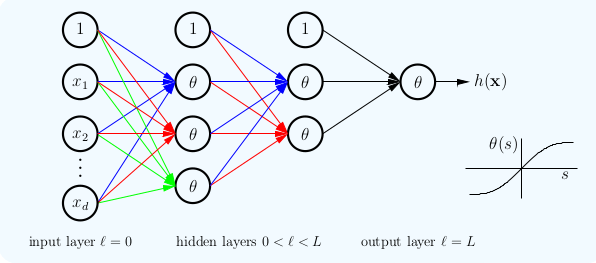
\includegraphics[scale=0.6]{img/grafo RRNN.png}
        \caption{Red Neuronal representada mediante un grafo. Imagen obtenida de \cite{data}. Notamos que el nodo del sesgo no le llega ninguna entrada}
        \label{fig:grafo rrnn prealimentada}
    \end{figure}
    
    La redes neuronales están organizadas en capas donde en cada una de ellas está comprendida por un conjunto de neuronas. El conjunto de neuronas $V$ se puede descomponer como unión disjunta de subconjuntos de neuronas, $V = \uplus V_{\ell=0}^L$ tal que cada subconjunto corresponde a los nodos de una única capa oculta. La arista en $E$ conecta algún nodo de $V_{\ell-1}$ con otro nodo de $V_{\ell}$ para algún $\ell \in [L]$. La capa $\ell = 0$ será llamada capa de entrada y contendrá $n+1$ neuronas donde $n$ es la dimensión del vector de entrada y la neurona restante será llamada sesgo y siempre contendrá el valor $1$. La última capa, $\ell = L$, es la capa de salida y determina el valor de la función. Finalmente las capas del medio serán llamadas capas ocultas. Usaremos el superíndice $\ell$ para referirnos a la capa, cada capa tiene dimensión $d^{(l)}$ que son el número de nodos presentes en la capa $\ell$. En la imagen \ref{fig:grafo rrnn prealimentada} podemos ver una representación gráfica de una pequeña red neuronal de cuatro capas. \\
    
   
    \begin{figure}[H]
        \centering
        \includegraphics[scale=0.8]{img/nodo nn.png}
        \caption{Interconexión entre dos nodos de dos capas contiguas. Fuente \cite{data}}
        \label{fig:nodo nn}
    \end{figure}
    
    
     Hagamos un poco de zoom sobre la topología de dos neuronas conectadas (Fig. \ref{fig:nodo nn}). En ella podemos ver dos nodos, representados por $i$ y $j$ en las capas $\ell -1$ y $\ell$ respectivamente. El nodo $v^{\ell}_j$ recibe una entrada, $s^{\ell}_j$, y emite una salida, $x^{\ell}_j$. La entrada $s^{\ell}_j$ consta de la salida del nodo $v^{\ell -1}_i$ de la capa anterior, $x^{\ell-1}_i$, multiplicado por los pesos asociados al enlace de ambos nodos, $w^{\ell}_{i,j}$.
    
    \begin{figure}[H]
        \centering
        \includegraphics[scale=0.8]{img/nodos nn.png}
        \caption{Interconexión entre capas ocultas. Fuente \cite{data}}
        \label{fig:nodos nn}
    \end{figure}
    
    
    La imagen \ref{fig:nodo nn} hace referencia a dos nodos conectados, pero en las redes neuronales son totalmente conectadas, es decir, todos los nodos de una capa se conectan con todos los nodos de la siguiente, por lo que la imagen \ref{fig:nodo nn} evoluciona a la imagen \ref{fig:nodos nn}. De esta manera, tenemos que la entrada a la capa $\ell$, $s^{\ell}$,  tiene dimensión $d^{\ell}$. La salida de esa misma capa, $x^{\ell}$, tiene dimensión $d^{\ell} + 1$. Los pesos de cada enlace los agrupamos en una matriz, $W^{\ell}$, con dimensión $(d^{\ell -1} + 1)\times d^{\ell}$. \\
    
    Una hipótesis $h \in \Hc_{NN}$ depende primordialmente de los pesos entre los enlaces, por lo que usualmente se denota como $h(x;w) = X^L$ donde $x = \{W^1,...,W^L\}$, enfatizando así la importancia de estos. \\
    
    Formalicemos la definiciones de conjunto de hipótesis de las redes neuronales, $\Hc_{NN}$ y redes neuronales prealimentadas. \\
    
    \begin{definicion}[Conjunto de hipótesis]
    Sea $L \in \N$, $d =(d^0,...,d^L) \in \N^L$, $W=(W^1,...,W^L)$ con $W^{\ell} \in \R^{(d^{\ell} + 1)\times d^{\ell}}$. El espacio de hipótesis de las redes neuronales prealimentadas viene dado por,
    \begin{equation}
        \Hc_{NN} = \{ h(x,W) : (L,d,W,\{\theta_t\}) \; implementa  \; h(x,W) = x^{(L)} \}
    \end{equation}
    \end{definicion}

    \begin{definicion}[Red Neuronal Prealimentada]
    Sea $L \in \N$, $d =(d^0,...,d^L) \in \N^L$, $W=(W^1,...,W^L)$ con $W^{\ell} \in \R^{(d^{\ell} + 1)\times d^{\ell}}$. Sean el conjunto de funciones $\{\theta^{\ell}: \ell \in \{1,...,L\}\}$ con $\theta$ una función de clase uno con valores de $\R^{d^{\ell-1}}$ en $\R^{d^{\ell}}$. Se define una red neuronal prealimentada como la cuaterna $[L,d,W,\{\theta^{\ell}\}]$ que implementa la función $h(x,W) = x^L$ a través de una conjunto finito de pasos de cálculo partiendo de unas condiciones iniciales,
    
    \begin{equation}
        \left\{ 
        \begin{array}{cc}
             
             
             x^0 = x & x \in \R^{d_0} \\
             
             x^{\ell} = \theta^{\ell}(s^{\ell}) & \ell \in \{1,...,L\} 
        
        \end{array}
        \right.
    \end{equation}
    
%    \begin{equation}
%        \left\{ 
%        \begin{array}{cc}
%             x^0 = 
%                \begin{bmatrix}
%                    1 \\ \theta^{\ell} (s^{\ell})
%                \end{bmatrix} 
%                & x \in \R^{d_0} \\
%             
%             x^{\ell} = 
%                 \begin{bmatrix}
%                    1 \\ \theta^{\ell}(s^{\ell}) 
%                 \end{bmatrix}
%             & \ell \in \{1,...,L\} 
%        \end{array}
%        \right.
%    \end{equation}
    
    \noindent donde
    \begin{equation}
        s^{\ell} = W^{\ell} x^{\ell - 1} + b^{\ell} \quad \ell \in \{1,...,L\}
    \end{equation}
    \end{definicion}


\section{Entrenamiento de Redes Neuronales}

    Cuando usamos una red neuronal que acepte una entrada $x_0$ y produzca una salida $x^L$, la información fluye hacia adelante a través de la red. La entrada $x_0$ proporciona la información inicial que luego se propaga a la unidades ocultas de cada capa para producir $x^L$. A esto se le llama \textit{forward propagation} o propagación hacia adelante. \\
    
    Durante el entrenamiento, este proceso tendrá una función de coste asociada $J$ que dependerá esencialmente de los pesos. El objetivo es calcular los pesos óptimos que minimizan dicha función. El algoritmo back-propagation permite que la información de la función de coste viaje hacia atrás a través de la red para calcular el gradiente. Este método surge de la necesidad de calcular de manera eficiente el gradiente ya que su principal inconveniente es su complejidad computacional. \\
    
    El back-propagation será usado en el algoritmo gradiente descendente, el cual se encarga de optimizar el valor de los pesos para minimizar así la función de coste. Este algoritmo requiere el cálculo del gradiente en cada iteración para movernos en dirección contraria. \\
    
    
    Antes de adentrarnos en faena con el entrenamiento de la red neuronal, comentemos algunas otras consideraciones importantes a tener en cuenta del entrenamiento. 
    \begin{itemize}
        \item \textit{Inicialización de los pesos}: Nunca se inicializan los pesos con valor cero o al mismo valor ya que de esa manera no habrá movimiento hacia el óptimo local en el gradiente descendente. Tampoco se deberán inicializar con valores muy grandes porque saturarían a la función sigmoidal y el gradiente se iría a cero. Lo correcto es una inicialización a pequeños valores aleatorios dados por una distribución gaussiana, $\mathcal{N}(0,\sigma_{\e}^2)$, de media cero y varianza $\sigma_{\e}^2$ cumpliendo $\sigma_{\e}^2 \underset{x_i}{max} || x_i||^2 << 1$. Para clasificación suele ser buena idea inicializar los pesos al valor obtenido después de aplicar un modelo de regresión. \\
        \item \textit{Criterio de parada}: Este criterio es de vital importancia para no aumentar de manera excesiva la complejidad en tiempo del entrenamiento. Hay muchos criterios tales como un número máximo de iteraciones, tamaño del gradiente, valor alcanzado en el error. Lo recomendable es usar una combinación de estos criterios.
    \end{itemize}
    
    
\subsection{Calculo del gradiente: Back-Propagation}

  El término back-propagation se suele malentender erróneamente como todo el algoritmo de aprendizaje de las redes neuronales. El back-propagation es un método para calcular el gradiente de manera eficiente para su posterior aplicación en el método del gradiente descendente o similares. Otro malentendido sobre el back-propagation es que solo se usa para calcular el gradiente de las redes neuronales, y esto tampoco es así. Es un método general, que además de emplearse en las redes neuronales se puede emplear en otros ámbitos ya que calcula las derivadas de cualquier función. En particular, calcula el gradiente $\nabla_{x}f(x,y)$ de una función arbitraria $f$, donde $x$ es un conjunto de variables las cuales queremos derivar, e $y$ es un conjunto de variables de las cuales depende la función pero no queremos derivar. En machine learning, el gradiente que se suele calcular es el de la función de coste, pero este algoritmo no tiene por qué usarse particularmente ahí. Si otras tareas de ML requieren calcular las derivadas de otras funciones, también puede emplearse esta técnica. El back-propagation puede generalizarse para salidas múltiples, pero para una mayor simplicidad, vamos a considerar que $f$ solo tiene una salida. \\ 
        

    Este algoritmo consiste en aplicar la regla de la cadena en cada nodo del grafo computacional para calcular el gradiente de manera eficiente. Se logra la eficiencia gracias a que no se repiten cálculos ya realizados y a una reordenación de los mismos. \\
        
    Para entenderlo mejor, vamos a dar un pequeño ejemplo de como se haría para el caso de un grafo computacional sencillo y después lo extenderemos al caso de redes neuronales. Considerar un grafo computacional cuya salida es un único escalar denotado como $u$. Queremos calcular el gradiente con respecto a los $n$ nodos del grafo denotados como $u^{(i)}$ con $i \in \{1,2,...,n\}$.  En otras palabras, queremos calcular $\frac{\partial u}{\partial u^{(i)}}$ para todo $i \in \{1,...,n\}$. Como ejemplo, vamos a considerar el grafo computacional de la figura \ref{fig:bp_grafo} donde cada nodo es una variable de entrada y se tiene $w, \; u^{(2)} = x = f(w), \; u^{(3)} = y = f(x)$ y $z = f(y)$ siendo esta última la variable de salida. \\
        
        \begin{figure}[htpb]
            \centering
            \includegraphics[scale=0.5]{img/backpropagation1.png}
            \caption{Grafo computacional que resulta del cálculo de la función f(f(f(w))) siendo $w \in \mathbb{R}$ y $f:\mathbb{R} \rightarrow \mathbb{R}$ una función real de variable real. Esta figura muestra el problema de la repetición de operaciones cuando se calcula el gradiente.}
            \label{fig:bp_grafo}
        \end{figure}
        
        \begin{figure}[htpb]
            \centering
            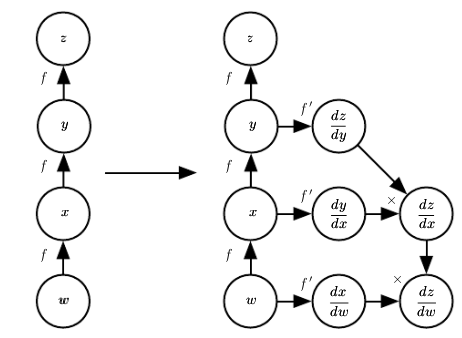
\includegraphics[scale=0.5]{img/grafo2.png}
            \caption{(Izquierda) Grafo que representa la función compuesta $z = f(f(f(w))). (Derecha)$ Grafo tras aplicar el algoritmo de \textit{back-propagation}. Este grafo representa el resultado deseado.}
            \label{fig:bp_grafo2}
        \end{figure}
        
    Para calcular $\frac{\partial z}{\partial w}$ aplicamos la regla de la cadena obteniendo
        
        \begin{equation}
            \begin{aligned}
                    \frac{\partial z}{\partial w} & = \frac{\partial z }{\partial y}\frac{\partial y}{\partial x}\frac{\partial x}{\partial w}\\
                    & = f'(y) f'(x) f'(w) \\
                    & = f'(f(f(w))) f'(f(w)) f'(w)
            \end{aligned}
        \end{equation}
        
    \noindent donde se observa que se realizan algunos cálculos repetidos, en este caso, se evalúa dos veces la función $f$ en la variable $w$. Si el grafo fuera mucho más complejo, tendríamos muchos más de estos cálculos repetidos provocando una disminución del tiempo considerable a la hora de computarlo. Se podría mejorar la eficiencia en tiempo si en memoria se guardarse el valor de estos cálculos y se usasen para operaciones futuras. \\
        
    Vamos a suponer que los nodos del grafo están ordenados y en cuyo caso podremos calcular la salida una detrás de otra. Cada nodo $u^{(i)}$ está asociado a una operación $f^{(i)}$ y se calcula evaluando la función 
        
        \begin{equation}
            u^{(i)} = f(\mathbb{A}^{(i)}) 
        \end{equation}

    \noindent donde $\mathbb{A}^{(i)}$ es el conjunto de todos los nodos padres que intervienen en el cálculo de la expresión $u^{(i)}$. También llamaremos por $Pa(u^{(i)}) = \{ j \; : b^{(j)} \in \mathbb{A}^{(i)}\}$ al conjunto de los índices de los nodos padre de $u^{(i)}$. Para el cálculo de las distintas derivadas usaremos la regla de la cadena
        
        \begin{equation}
            \frac{\partial u}{\partial u^{(j)}} = \sum_{i/j \in Pa(u^{(i)})} \frac{\partial u}{\partial u^{(i)}} \frac{\partial u^{(i)}}{\partial u^{(j)}}
        \end{equation}
        
    Llamamos $\mathcal{G}$ al grafo de cómputo de la función $f$, en nuestro ejemplo sería el grafo de la figura \ref{fig:bp_grafo}. Para realizar \textit{back-propagation} podemos construir un grafo computacional que depende de $\mathcal{G}$ y en donde añadimos nodos extra. Denotamos a dicho grafo como $\mathcal{B}$, los cálculos en $\mathcal{B}$ se realizan con el orden inverso que tienen en $\mathcal{G}$ y cada nodo de $\mathcal{B}$ calcula la derivada $\frac{\partial u}{\partial u^{(i)}}$ asociada al grafo hacia adelante del nodo $u^{(i)}$. El grafo $\mathcal{B}$ contiene exactamente una arista por cada arista que tenga $\mathcal{G}$ desde el nodo $u^{(j)}$ al nodo $u^{(i)}$, de este modo, si desde el nodo $u^{(j)}$ al nodo $u^{(i)}$ hay 5 aristas, entonces el nuevo grafo contendrá $5$ nodos extra enlazados con sus respectivas aristas, cada nodo representa una derivada. La arista de $u^{(j)}$ a $u^{(i)}$ está asociada al cálculo de $\frac{\partial u^{(i)}}{\partial u^{(j)}}$. Además, se realiza un producto para cada nodo entre el gradiente calculado y respecto a los nodos $u^{(i)}$ que son los hijos del nodo $u^{(j)}$. En nuestro ejemplo, el cálculo del grafo $\mathcal{B}$ quedaría como el de la imagen (derecha) de \ref{fig:bp_grafo2}. A continuación vamos a mostrar un algoritmo de una versión simplificada del \textit{backpropagation} que calcula las derivadas de $u^{(n)}$ con respecto a las variables en el grafo. \\
    
    En el contexto de redes neuronales, se calcula el gradiente con respecto los pesos $W$ y los sesgo $b$ de la función de coste $J(w,b) = \frac{1}{N} \sum_{i=1}^N \ell(h_{w,b},y_i) + \lambda \Omega(w,b)$ con $w = [W_1,...,W_L]$ donde el segundo sumando indica el término de regularización. Para una mayor simplicidad vamos a incluir los sesgos en el vector $W$ tomando como índice el cero, por lo que el vector $x$ en este caso tendrá una componentes más con valor constantemente igual a $1$. \\
	  
	
    \subsubsection{Propagación hacia adelante (Feed Forward)}
        
        Esta es la primera parte del algoritmo, cuya finalidad principal es calcular el grafo $\mathcal{G}$ \eqref{eq:grafo feed forward} que en términos de redes neuronales se traduce en calcular la función que implementa la red neuronal. \\
        
        \begin{equation} \label{eq:grafo feed forward}
            x^0 \overset{W^1}{\longrightarrow} s^1 \overset{\theta^1}{\longrightarrow} x^1 \overset{W^2}{\longrightarrow} s^2 \overset{\theta^2}{\longrightarrow} x^2 \cdots x^{L-1} \overset{W^L}{\longrightarrow} s^L \overset{\theta^L}{\longrightarrow}x^L
        \end{equation}
        
        	\begin{algorithm}[H]
        	\label{alg:forward}
	        \caption{Propagación hacia adelante para calcular la función de coste a través de una red neuronal profunda típica}
	        \KwData{$L$: Network Deep}
	        \KwData{$x$: input}
	        \KwData{$y$: target}
	        \KwData{y: target}
	        \KwData{$\{\theta^i\}: i \in \{1,...,L\}$}
	        \KwData{$W^i$: $i \in \{0,1,...,L\}$ matrices de pesos (con sesgos)}
	        \KwResult{$(x_i)_{1,...,L},(s_i)_{1,...,L}$}
	        
	        $x^0 \leftarrow x$ \; 
	        \ForEach{$k \in \{1,...,L\}$}{
	            $s^k \leftarrow  W^k x^{k-1}$\;
	            $x^k \leftarrow \begin{bmatrix}
                    1 \\ \theta^{\ell} (s^{\ell})
                \end{bmatrix} $\;
	            }
	       $h(x,W) \leftarrow x^L$\;
	       $J = L(h(x,W),y) + \lambda \Omega(W)$
	       \end{algorithm}
	       
	                       
	       
	       
	       \begin{figure}[H]
	           \centering
	           \includegraphics[scale=0.7]{img/propagacion forward.png}
	           \caption{Representación de la propagación hacia adelante en una red neuronal prealimentada}
	           \label{fig:esquema forward}
	       \end{figure}
        
        
    \subsubsection{Propagación hacia atrás (Back-Propagation)}
        
        
        Antes de entrar de lleno con el algoritmo, especifiquemos la notación. Definimos la \textit{sensibilidad} como
        
        \begin{equation}\label{eq:sensibity}
            \delta^{\ell} = \frac{\partial L}{\partial s^{\ell}}
        \end{equation}
        
        \noindent La sensibilidad cuantifica cómo cambia $L$ con respecto a $s^{\ell}$. Usando la sensibilidad podemos escribir la derivada parcial con respecto la matriz de pesos $W^{\ell}$ como,
        
        \begin{equation}\label{eq:partial L partial W}
            \frac{\partial L}{\partial W^{\ell}} = \frac{\partial L}{\partial s^{\ell}} \frac{\partial s^{\ell}}{\partial W^{\ell}} = x^{\ell - 1}(\delta^{\ell})^T
        \end{equation}
        
        

        
        
        \noindent La derivada parcial del término de la izquierda es una matriz de dimensión ${(d^{\ell -1} + 1)\times d^{\ell}}$ y no es difícil probar que dicha matriz se obtiene con el producto de los dos vectores del término de la derecha. La imagen \ref{fig:backpro esquema} muestra que en la salida de la capa $\ell + 1$ el vector $\delta^{\ell + 1}$ el cual es multiplicado por la matriz de pesos $W^{\ell + 1}$ se suma y se le pasa como entrada a las neuronas de la capa $\ell$. Estos nodos multiplican dicha entrada por el jacobiano $(J_{\theta^{\ell}})_{s^{\ell}}$ para obtener $\delta^{\ell}$. Denotando $\odot$ la multiplicación elemento a elemento de dos vectores tenemos que,
        
        \begin{equation}
            \delta^{\ell} = (J_{\theta^{\ell}})_{s^{\ell}} \odot [W^{\ell + 1} \delta^{\ell + 1}]_1^{d^{\ell}}
        \end{equation}
        
        \noindent donde el vector $[W^{\ell + 1} \delta^{\ell + 1}]_1^{d^{\ell}}$ representa las componentes $1,...,d^{\ell}$ del vector $W^{\ell + 1} \delta^{\ell + 1}$ excluyendo la componente del sesgo la cual tiene índice cero. Esta fórmula no es nada extraña ni la hemos sacado de la manga. La sensibilidad del error en la capa $\ell$ es proporcional a la pendiente de la función de activación de la capa $\ell$ (mayor pendiente significa que un pequeño cambio en $s^{\ell}$ tendrá un mayor impacto en $s^{\ell + 1}$), al tamaño de los pesos que salen de la capa (mayores pesos significan que un menor cambio en $s^{\ell}$ tendrá más impacto en $s^{\ell + 1}$) y a la sensibilidad de la capa siguiente ( un cambio en la capa $\ell$ afecta a la entrada de la capa $\ell + 1$ así que si el error es mas sensible a la capa $\ell + 1$ entonces tendrá aún más sensible a la capa $\ell$). \\
        
   
        La salida de capa capa $x^{\ell}$ se calcula en la propagación hacia adelante usando la salida de la capa anterior $x^{\ell - 1}$. Para calcular la sensibilidades basta con recorrer el grafo de la red neuronal hacia atrás ya que para calcular $\delta^{\ell}$ necesitamos $\delta^{\ell + 1}$. Esta idea se muestra en la figura \ref{fig:backpro esquema}, quedando el grafo computacional de la siguiente manera
        
        \begin{equation}
            \delta^{1} \leftarrow \delta^{2} \cdots \leftarrow \delta^L
        \end{equation}
   
        \begin{figure}[htpb]
            \centering
            \includegraphics[scale=0.7]{img/backpro esquema.png}
            \caption{Representación esquemática de la propagación hacia atrás}
            \label{fig:backpro esquema}
        \end{figure}
        
        El algoritmo queda como sigue,
        
        \begin{algorithm}[H]
	       \label{alg:feedforward}
	        \caption{Propagación hacia atrás}
	        \KwData{$[L,d,W,b,\{\theta^i\}]$ red neuronal prealimentada}
	        \KwData{$x$: input}
	        \KwData{$y$: target}
	        \KwData{y: target}
	        \KwResult{$\nabla_W L$}
	        
	        $(s^i)_{1,...,L},(x^i)_{0,...,L} \leftarrow ForwardPropatagion$ \;
	        $\delta^L \leftarrow \frac{\partial L}{\partial s^L}$ \; 
	        \ForEach{$\ell$ $\in$ $\{L-1,...,1\}$}{
	            $\delta^{\ell} = (J_{\theta^{\ell}})_{s^{\ell}} \odot [W^{\ell + 1} \delta^{\ell + 1}]_1^{d^{\ell}}$\;
	            $\frac{ \partial L}{\partial W^{\ell}} = x^{\ell - 1} (\delta^{\ell})^T$
	            }
	   \end{algorithm}
        

    \subsection{Optimización a través del Gradiente descendente}

    Fijada una función de coste y un algoritmo eficiente para el cálculo del gradiente introducimos el método de optimización que se aplica en las redes neuronales, el gradiente descendente. Este método fue propuesto inicialmente en $1847$ por Cauchy \cite{cauchy1847methode}, y no fue hasta casi 100 años después que se demostró su convergencia gracias a Haskell Curry \cite{curry1944method}. \\
    
    La intuición geométrica que subyace detrás de esta técnica es la siguiente. Veamos la función que queremos minimizar como una superficie en el espacio. En un instante de tiempo cero, partimos de la posición $w(0)$ de la superficie, y en cada instante de tiempo nos vamos moviendo sobre ella. El objetivo es descender de la superficie hasta llegar un punto en el que nos movamos en la dirección en la que nos movamos, no consigamos descender más. También podemos considerar el movimiento de descenso como aquel que haría una pelota si la colocásemos en una superficie $2$-dimensional gracias a la gravedad, ésta descendería hasta llegar a un punto de equilibro, entendido como un mínimo local. \\
    
    Vamos a considerar un campo escalar $f:S \subset \R^n \to \R$ continuo y derivable en su dominio con derivada continua en el interior de $S$. Su función gradiente $\nabla f$ es un campo vectorial y apunta en la dirección en que la derivada direccional es máxima por lo que la dirección en la que la función desciendo más rápido viene dada por,
    
    \begin{equation}
        -\eta \nabla f(w_1,...,w_n) = -\eta \Big( \frac{\partial f}{\partial w_1} (w_1,...,w_n),...,\frac{\partial f}{\partial w_n}(w_1,...,w_n) \Big)
    \end{equation}

    \noindent donde $\eta$ es un factor de proporcionalidad más conocido en el mundo del aprendizaje automático como tasa de aprendizaje. De este modo el algoritmo consiste en partir de unas condiciones iniciales $w_0$ y de manera iterativa calcular el vector opuesto del gradiente y avanzar en esa dirección una distancia marcada por la tasa de aprendizaje. Las ecuaciones quedan como siguen,
    
    \begin{equation}
        w_i = x_{i-1} - \eta \nabla f(w_{i-1}) \qquad w_i \in \R^n 
    \end{equation}


    Hay que tener siempre en mente que cuando aplicamos esta técnica, obtendremos un mínimo local que por lo general no será global. \\
    
    \subsubsection{Variantes del gradiente descendente}
    
    En el panorama del aprendizaje automático, tendremos un conjunto de entrenamiento conformado por varios elementos (vectores) por lo que calcularemos la media aritmética de los gradientes de la función de pérdida para cada uno de esos elementos. Para ello, evaluaremos la función de coste para cada ejemplo de entrenamiento antes de actualizar el gradiente, lo que computacionalmente en tiempo es una barbaridad. Como contramedida, solo se emplea un solo ejemplo de entrenamiento en cada actualización, esta variación del gradiente descendente recibe el nombre de \textit{gradiente descendente estocástico}. \\
    
    
        \begin{algorithm}[H]
	       \label{alg:SGD}
	        \caption{Gradiente Descendente Estocástico (SGD)}
	        \KwData{$W_0$ condiciones iniciales}
	        \KwData{$\eta$: tasa de aprendizaje}
	        \KwData{$S$: conjunto de entrenamiento}
	        \KwData{$L$: función de perdida}
	        \KwData{$n\_epochs$: numero de epocas}
	        \KwResult{$w$ pesos finales}
	        

    	       \ForEach{$(x,y)$ $\in$ $S$}{
    	           $w \leftarrow w - \eta \nabla L(h(x,w),y)$
    	           }
	           
	   \end{algorithm}
	   
	   
	 Esta variación del gradiente descendente nos sitúa en el extremo opuesto que la versión en donde se evalúan todos los ejemplos de entrenamiento y aplicamos la media. Por lo que esta aproximación no va a ser tan fidedigna como la otra, así que, como alternativa surgió el \textit{descenso del gradiente estocástico con minilotes}. Consideramos una partición disjunta del conjunto de entrenamiento y a cada subconjunto lo llamamos minilote. Entonces este método consiste en actualizar los pesos una vez se haya evaluado todos los ejemplos de dicho minilote. Así según el tamaño del minilote, buscamos un compromiso entre la robustez del gradiente descendente y la eficiencia del SGD. \\
	 
	 Algo a tener en cuenta y a lo cual le hemos restado importancia hasta ahora es la tasa de aprendizaje $\eta$. Su correcto valor es un factor clave, en la en la imagen $\ref{fig:lr}$ podemos ver distintos escenarios según su valor. Una tasa de aprendizaje pequeña consigue que el gradiente descendente avance poco a poco necesitando muchas iteraciones para la convergencia. Una tasa de aprendizaje grande, puede ocasionar que la convergencia sea inestable o incluso saltarnos el óptimo. Otro escenario es que la tasa de aprendizaje sea una función que vaya variando, de tal modo que al principio tenga valores grandes para acelerar la convergencia y conforme avanzamos en iteraciones tome valores pequeños para no escaparnos del óptimo. \\
	 
	 Este última método motiva una amplia gama de variaciones en el gradiente descendente que se centran en cómo modificar la tasa de aprendizaje. De este modo surgen variantes como AdaGrad, Adam, RMSProp...
	 
	 \begin{figure}[H]
	     \centering
	     \includegraphics[scale=0.5]{img/learningrate.png}
	     \caption{Escenarios que presenta la elección de la tasa de aprendizaje}
	     \label{fig:lr}
	 \end{figure}


       
        
        
\section{Función de Activación}
    
    Las funciones de activación son transformaciones que por lo general son no lineales que se aplican al producto escalar de los pesos por las características en cada neurona para dar la salida. La no linealidad aporta una mayor variedad y mejores aproximaciones. Veamos las más comunes usadas en la práctica. \\
    
    \begin{center}
        \textbf{Función sigmoidal} \\
    \end{center}
    
        Esta función es de la forma
        
        \begin{equation}
            \sigma(x) = \frac{1}{1 + e^{-x}}
        \end{equation}
        
        \noindent y claramente es no lineal. Tiene por dominio la recta real, pues el denominador no se anula en ningún punto, haciéndola una función continua, además es diferenciable. Toma valores en el intervalo $[0,1]$ y presenta dos asíntotas horizontales en el infinito,
        
        \begin{equation}
            \sigma(x) \overset{x \to -\infty}{\longrightarrow}  0 \qquad  \sigma(x)\overset{x \to \infty}{\longrightarrow}  1
        \end{equation}
        
        Esta función es muy útil pues la podemos emplear para transformar un escalar en una probabilidad colapsando a cero o a uno según la magnitud de éste, por este motivo se suele emplear en la capa de salida (aunque también es común usarla en las neuronas de las capas ocultas). La gráfica la presentamos en la figura \ref{fig:grafica sigmoidal}. \\
        
        Un inconveniente es que estas funcionan saturan y destruye los gradiente durante el proceso de entrenamiento. Esto es debido a que cuando la neurona satura el producto escalar en algunas de las colas, ya sea $0$ ó $1$ el gradiente en esas regiones es prácticamente nulo. Durante el proceso de retropropagación, puede resultar bastante peligroso por lo que se podría desvanecer. \\
        
        Por otro lado y relacionado con el motivo anterior, hay que ser muy cuidadosos con la inicialización de los pesos de las neuronas que usen este tipo de función de activación para evitar dicha saturación en las colas. Ya que si los pesos son muy grandes en términos absolutos, la red no va a aprender debido al desvanecimiento del gradiente. \footnote{El problema del desvanecimiento del gradiente lo comentaremos en el capítulo de Redes Neuronales Recurrentes, para más información ir a la sección \ref{seccion:sorpresa}} \\
        
        Otro problema es que la salida no está centrada en el cero, esto puede originar un comportamiento indeseado en las actualizaciones del gradiente de los pesos. \\
        
        \begin{figure}[H]
            \centering
            \includegraphics[scale=0.5]{img/sigmoide.png}
            \caption{Gráfica función sigmoidal. \href{https://ml4a.github.io/images/figures/sigmoid.png}{Fuente}}
            \label{fig:grafica sigmoidal}
        \end{figure}
        
        
        
        
        
    \begin{center}
        \textbf{Función tangente hiperbólica} \\
    \end{center}
    
        La gráfica de la función la presentamos en \ref{fig:grafica tanh}. Es otra función no lineal cuya expresión viene dada por 
        
        \begin{equation}
            \tanh(x) = \frac{e^x - e^{-x}}{e^x + e^{-x}}
        \end{equation}
        
        \noindent también la podemos poner en términos de la función sigmoidal,
        
        \begin{equation}
            \tanh(x) = 2 \sigma(2x) - 1
        \end{equation}
        
        Al igual que la función sigmoidal, tiene de dominio toda la recta real, pero ahora los valores que toma están comprendidos en el intervalo $[-1,1]$ presentando una asíntota vertical en el infinito hacia esas colas, esto es,
        \begin{equation}
            \tanh(x) \overset{x \to -\infty}{\longrightarrow}  -1 \qquad  \tanh(x)\overset{x \to \infty}{\longrightarrow}  1
        \end{equation}
        
        \noindent Esta vez, tenemos que la función está centrada en el cero, por lo que aunque la salida de esta función se sature no tendremos el problema que comentamos con la función sigmoidal sobre el comportamiento indeseado en la actualización del gradiente de los pesos. Por este motivo se prefiere la no linealidad de esta función frente a la sigmoidal, aunque sea un simple escalado de la anterior. \\
    
        \begin{figure}[H]
            \centering
            \includegraphics[scale=0.3]{img/tanh.png}
            \caption{Gráfica función tangente hiperbólica \href{https://production-media.paperswithcode.com/methods/Screen_Shot_2020-05-27_at_4.23.22_PM_dcuMBJl.png}{Fuente}}
            \label{fig:grafica tanh}
        \end{figure}
        
        
    \begin{center}
        \textbf{Función ReLu} \\
    \end{center}
    
        La unidad lineal rectificada se ha hecho muy popular en los últimos años. Su expresión viene dada por
        \begin{equation}
            f(x) = max(0,x)
        \end{equation}
        
        \noindent Esta función se puede ver como un simple umbral en cero. Su gráfica viene dada por la imagen \ref{fig:grafica relu}. El uso de esta función de activación presenta varias ventajas así como desventajas.
        
        \begin{itemize}
            \item Ventajas:
            \begin{enumerate}
                \item Acelera en gran medida la convergencia del escenso del gradiente estocástico en comparación con las funciones tanh y sigmoidal debido a su forma no lineal y a no saturar los valores.
                \item En comparación con otras funciones de activación que implican operaciones costosas como exponenciales, esta función se puede implementar de manera muy simple y con poco coste.
            \end{enumerate}
            \item Desventajas: Estas funciones pueden ser frágiles durante el entrenamiento y pueden desvanecerse. Por ejemplo, imaginemos un gradiente que discurra por una neurona con esta función de activación, podría darse el caso en el que los pesos se actualicen de manera que la neurona no vuelva a activarse en ningún punto. Si esto pasara, entonces el gradiente que pasa por esta neurona será siempre nulo a partir de ese punto. Se ha llegado a observar en algunos casos que hasta el $40\%$ de la red puede desvanecerse, esto es, neuronas que nunca se activan en todo el conjunto de datos de entrenamiento en el caso de que la tasa de aprendizaje sea algo elevada. Para un ajuste adecuado de la tasa de aprendizaje, esto no debiera de ocurrir con tanta facilidad.
            
        \end{itemize}
    
    
        \begin{figure}[H]
            \centering
            \includegraphics[scale=0.55]{img/relu.png}
            \caption{Gráfica función ReLu \href{https://miro.medium.com/max/357/1*oePAhrm74RNnNEolprmTaQ.png}{Fuente}}
            \label{fig:grafica relu}
        \end{figure}
        
        
    \begin{center}
        \textbf{Función Leaky ReLu} \\
    \end{center}
    
        Esta función de activación cuya gráfica la podemos encontrar en la imagen \ref{fig:leakyrelu} es un intento de solucionar el problema de la ReLu comentado anteriormente. En lugar de que la función tome el valor cero, tomará una pequeña pendiente positiva. La expresión viene dad por
        \begin{equation}
            f(x) = max(\alpha x, x)
        \end{equation}
        \noindent donde $\alpha$ es una constante que suele tomar valores del orden de $10^{-3}$
        

        
        \begin{figure}[H]
            \centering
            \includegraphics[scale=0.55]{img/leakyrelu.png}
            \caption{Gráfica función Leaky ReLu \href{https://miro.medium.com/max/398/1*FDOyQlRurCK7mWU5i0Ly_w.png}{Fuente}}
            \label{fig:leakyrelu}
        \end{figure}
    
    \begin{center}
        \textbf{Otras Variante de ReLu: Elu y Selu} \\
    \end{center}
    
        La función Leaky ReLu no es la única alternativa que se propuso frente a ReLu, tenemos otras muchas variantes como Elu y Selu. Sus gráficas las podemo ver en la figura \ref{fig:grafica variante relu}. La función Elu viene dada por 
        \begin{equation}
            Elu(x) = max(\alpha(e^x -1),x)
        \end{equation}
        
        \noindent donde $\alpha > 0$ es una contante que al igual que el caso de la funcón Leaky Relu, toma valores pequeños. En cambio la función Selu viene dada por 
        
        \begin{equation}
            Selu(x) = max(\alpha \lambda(e^x - 1,x))
        \end{equation}
        
        \noindent donde $\lambda \approx 1.0507$ y $\alpha \approx 1.6732$. 

        
        
        \begin{figure}[H]
            \centering
            \includegraphics[scale=0.4]{img/Variante ReLu.png}
            \caption{Variantes ReLu \href{https://www.researchgate.net/profile/Alberto-Marchisio/publication/328878703/figure/fig2/AS:691988286423047@1541994272922/Behavior-of-ReLU-ELU-and-SELU-activation-functions.ppm}{Fuente}}
            \label{fig:grafica variante relu}
        \end{figure}
    
    
    
    \begin{center}
        \textbf{Función MaxOut} \\
    \end{center}
    
    Es otro tipo de función de activación que generaliza la ReLu y su versión Leaky ReLu. Su expresión viene dada por 
    \begin{equation}
        maxout = max(w^T_1x+b_1,w^T_2x+b_2)
    \end{equation}
    
    \noindent Por lo que esta función de activación goza de todas las ventajas que presenta la ReLu y no tiene sus inconvenientes. Pero presenta un nuevo problema al duplicar los parámetros para cada neurona. 
    



\endinput


% !TeX root = ../libro.tex
% !TeX encoding = utf8



\setchapterpreamble[c][0.75\linewidth]{%
	\sffamily
  
    Las redes neuronales convolucionales es un caso particular de redes neuronales en las que entran en juego las capas de convolución. Estas redes se desarrollaron a finales del siglo pasado con el objetivo de reconocer objetos en imágenes. Poco a poco fueron ganando fama y popularidad dando un gran empuje a la visión por computador. La primera gran innovación en lo que respecta a estas redes fue protagonizada por Yann LeCun en 1990 con su propuesta LeNet. A partir de ahí comenzó una carrera por el desarrollo de estas redes. El fomento de la competitividad y la inversión que había en inteligencia artificial contribuyeron al avance de este área y surgieron grandes y prometedoras propuestas poco a poco. Destacamos las arquitecturas AlexNet (2012), creada por Alex Krizhevsky, Ilya Sutskever and Geoff Hinton. Poco después surgió ZF Net (Matthew Zeiler and Rob Fergus, 2013),GoogLeNet (2014) ,VGGN(Karen Simonyan and Andrew Zisserman, 2014),ResNet(Kaiming He et al., 2015). \\
    
    
    El propósito de este capítulo no es hacer una descripción detallada sobre este tipo de redes neuronales, si no más bien introducirlas al lector de tal manera que sea capaz de comprenderlas aunque no tenga conocimiento previo del tema. El capítulo comenzará con una breve introducción que expone el motivo por el que las redes neuronales prealimentadas no hacen de tan bien el trabajo destinado a las redes convolucionales. Después se explicará la operación fundamental que subyace dentro de estas redes, la convolución. Se verá la convolución para el caso de funciones continuas y discretas y se abordará en los casos unidimensionales y bidimensionales, tras lo se estudiará brevemente un ejemplo práctico. Tras entender esta importante operación, se introducirán los distintos tipos de capas presenten en estas redes, así pues se verán las capas convolucionales junto con algunas de sus propiedades, las capas de pooling, las capas de normalización y las totalmente conectadas. Se finalizará el capítulo con una explicación en cuanto a cómo diseñar una arquitectura para este tipo de redes.\\
    
    La principal referencia usada ha sido el contenido del libro \textit{Deep Learning Book} \cite{Goodfellow-et-al-2016} y el material proporcionado por la universidad de \href{http://cs231n.stanford.edu/}{Standford}
    
    
	\par\bigskip
}
\chapter{Redes Neuronales Convolucionales}\label{ch:CNN}

\newpage
\section{Introducción}

        En las redes neuronales, vimos que la información viaja a través de las capas ocultas desde la entrada hasta la salida y en donde las neuronas de una capa están totalmente conectadas a las neuronas de la anterior. Este tipo de redes neuronales, no presentan resultados deseados cuando se trabaja con imágenes. Supongamos una imagen de tamaño $(200,200,3)$, haciendo que la primera capa oculta tenga un total de $200 \cdot 200 \cdot 3 = 120000$ pesos. Pueden parecernos más o menos pocos en función de la capacidad hardware que tengamos, en cambio, las imágenes que usamos en la práctica, suelen ser mucho más grandes, haciendo que necesitemos millones y millones de pesos. Esto resulta un tanto inmanejable. \\
        
        Las redes neuronales convolucionales aprovechan el hecho de que la entrada es una estructura multidimensional y restringen la arquitectura de manera más sensata. En una red neuronal convolucional cuando se tratan imágenes las capas se disponen en una estructura de tres dimensiones (ancho, largo y profundidad). Además, las neuronas de una capa sólo estarán conectadas a una pequeña región de la capa anterior, en lugar de manera totalmente conectada y se irá reduciendo progresivamente la dimensión hasta llegar a la capa de salida, la cual tendrá una estructura unidimensional, es decir, de la forma $(1,1,depth)$. \\
        
        
\section{Operador Convolución}

    En el área de las matemáticas y en especial, en el campo del análisis funcional, una convolución es un operador el cual transforma dos funciones $f$ y $g$ en una tercera que en cierto sentido representa la magnitud en la que se superponen f y una versión trasladada e invertida de g. Demos una definición de convolución en la que las funciones $f$ y $g$ son funciones reales de variable real.
    
    \begin{definicion}[Convolución]\label{def:conv_1}
    Sean $f,g:\R \to \R$ dos funciones reales de variable real. Se define la convolución de $f$ y $g$, como 
    \begin{equation}
        (f*g)(t) = \int_{-\infty}^{\infty} f(x)g(t-x) \; dx
    \end{equation}
    \end{definicion}
    
    Una interpretación geométrica de la definición anterior es que la convolución expresa el área de $g$ que queda solapada por la función $f$ cuando $g$ se desplaza a través del eje de abcisas. Notamos que para aplicar la definición anterior a nivel práctico necesitamos de un sistema que sea continuo, lo cual no tendremos en nuestro caso por trabajar con señales temporales. Por lo que necesitamos una definición discreta de la convolución para el caso unidimensional.
    
    \begin{definicion}[Convolución Discreta Unidimensional]\label{def:conv_2}
    Sean $f,g:\mathbb{Z} \to \mathbb{Z}$ dos funciones con dominio y codominio en los enteros. Se define la convolución de $f$ y $g$ como
    \begin{equation}
        (f*g)(t) = \sum_{n \in \mathbb{Z}} f(n) g(t-n)
    \end{equation}
    \end{definicion}
    
    La definición de convolución discreta, así como la versión continua que dimos en \ref{def:conv_1} se puede extender a dimensión mayor. Por ejemplo, en imágenes se suelen trabajar con convoluciones $2$-dimensionales en la que la funciones $f$ y $g$ toman valores en $\mathbb{Z}\times\mathbb{Z}$ y la convolución se expresa como
    
    \begin{equation}\label{eq:conv_3}
        (f*g)(s,t) = \sum_{n \in \mathbb{Z}} \sum_{n \in \mathbb{Z}} f(n,m)g(s-n,t-m)
    \end{equation}



    En el contexto en el que aplicaremos esta operación, denotaremos a la función $f$ como $x$ la cual jugará el papel de \textit{entrada} (puede ser una imagen o una serie temporal) y a la función $g$ como $w$ y la llamaremos \textit{núcleo}, \textit{kernel} o \textit{filtro}. No nos vamos a meter en el terreno de la convolución y en todas las posibilidades que ofrece, solamente comentaremos que gracias a su propiedad conmutativa, podemos permutar las variables de $f$ y $g$. Por ejemplo, si trabajamos con la definición de convolución discreta unidimensional \ref{def:conv_2}, tenemos que
    
    \begin{equation}
        (x*w)(t) = \sum_{n \in \mathbb{Z}} x(t-n) w(n)
    \end{equation}

    \noindent si usamos la definición para el caso de dimensión $2$ dada por \eqref{eq:conv_3}, entonces tendríamos
    
    \begin{equation}
        (x*w)(s,t) = \sum_{n \in \mathbb{Z}} \sum_{n \in \mathbb{Z}} x(s-n,t-m)w(n,m)
    \end{equation}

    \noindent Esta nueva visión es algo más práctica, ya que podemos ver los cálculos  en términos de una expresión que actúa sobre todos los puntos de la entrada. Existe una operación similar a la convolución llamada correlación cruzada en la que la única diferencia es que en esta última no invierte el núcleo, de esta manera quedaría como 
    
    \begin{equation}
        (x*w)(t) = \sum_{n \in \mathbb{Z}} x(t+n) w(n)
    \end{equation}
    \noindent en el caso unidimensional, y 
    \begin{equation}
        (x*w)(s,t) = \sum_{n \in \mathbb{Z}} \sum_{n \in \mathbb{Z}} x(s+n,t+m)w(n,m)
    \end{equation}
    
    \noindent en el bidimensional. \\ 
    
    Esta operación la denotaremos igual que la convolución y en la práctica no distinguiremos cual estamos usando, ya que la red neuronal se dedica a aprender los pesos del kernel y si usa una u otra, solo le basta con invertir el núcleo. El motivo de presentar la correlación cruzada es que muchas librerías de aprendizaje la implementan en vez de la convolución por motivos de eficiencia. 
    
    
    \begin{ejemplo}[Ejemplo convolución]
    
    Veamos a continuación un ejemplo, para ello nos vamos a fijar en la imagen \ref{fig:ejemplo_conv}. Nuestra matriz de entrada es la matriz numérica bidimensional situada más a la izquierda de la fotografía y el kernel es la matriz $3\times 3$ situada a la derecha de la matriz de entrada. \\
    
    El proceso de convolución consiste superponer el núcleo en la imagen de entrada e ir calculando operaciones elementales (suma y multiplicación), tras ello, se desliza el kernel por la entrada y se vuelven a realizar los cálculos.
    
    \begin{figure}[H]
        \centering
        \includegraphics[scale=0.8]{img/convolucion.png}
        \caption{Ejemplo de convolución. \href{https://medium.com/@bdhuma/6-basic-things-to-know-about-convolution-daef5e1bc411}{Fuente}}
        \label{fig:ejemplo_conv}
    \end{figure}
    
    
    En una imagen de verdad, dependiendo de como sea el filtro, obtendriamos un resultado como en el de la imagen \ref{fig:ejemplo_conv2} en donde se ha aplicado el filtro derivada.
    
    \begin{figure}[H]
        \centering
        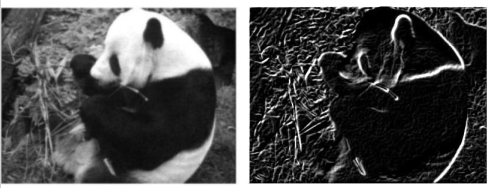
\includegraphics[scale=0.6]{img/ejemplo_conv2.png}
        \caption{(Izquierda) Imagen original. (Derecha) Imagen obtenida aplicando el filtro derivada}
        \label{fig:ejemplo_conv2}
    \end{figure}
    
    
    \end{ejemplo}
    
    
    La convolución es bastante útil porque presenta características clave que constribuyen a la mejora de un sistema de Machine Learning. 
    
    \begin{figure}[H]
        \centering
        \includegraphics[height=4cm, width=15cm]{img/redConv_1.png}
        \caption{(Izquierda) Una red neuronal con tres capas. (Derecha) Una red convolucional cuyas capas organizan las neuronas en tres dimensionas. Tal y como se visualiza, cada capa transforma el volumen de entrada $3$D en un volumen de salida también $3$D de las activaciones de las neuronas. La estructura rosa es la imagen de entrada.}
        \label{fig:red_conv_1}
    \end{figure}



\section{Capas usadas en redes convolucionales}

     \subsection{Capa convolucional}
  
        
        Una capa de convolución consiste en un conjunto de filtros que la red aprende. Cada filtro se extiende por la profundidad del volumen de la entrada. Durante la convolución deslizamos cada filtro a lo largo de la anchura y altura del volumen de entrada y calculamos los productos punto a punto entre las entre la imagen y el filtro. Al deslizar el filtro por la anchura y altura del volumen de entrada, producimos un mapa de salida bidimensional que da las respuesta de ese filtro en cada posición espacial. \\
        
        Intuitivamente, la red aprenderá filtros que se activan cuando ven algún tupo de característica visual como por ejemplo un borde o alguna mancha y conforme se va avanzando por la red estos patrones se volverán aún más complejos. Tendremos entonces un conjunto complejo de filtros en cada capa convolucional y cada uno de ellos producirá un capa de salida o activación bidimensional independiente. Se apilaran todos estos mapas a lo largo de la dimensión de profundidad dando lugar así al volumen de salida.  \\
        
        Comentemos a continuación los detalles de la conectividad de las neuronas, su organización en el espacio y su esquema de reparto de parámetros. \\
        
        \begin{center}
            \textbf{Disposición espacial}
        \end{center}
        
        La disposición espacial hace referencia a cuantas neuronas hay en el volumen de salida y a como están dispuestas. Hay tres hiperparámetros que controlan el tamaño de volumen de salida. La profundidad, la zancada y el zero-padding. \\
        
        La profundidad del volumen de salida corresponde al número de filtros que queremos usar, cada uno se especializa a buscar algo distinto en la entrada. Otro hiperparámetro es la zancada o paso, hace referencia a la zancada con la que deslizamos el filtro por la entrada. La zancada se mide por \textit{strides}. Un stride de uno indica que movemos el filtro unidad por unidad, en cambio, si es 3, entonces en cada deslizamiento, lo trasladamos tres posiciones. Así logramos volúmenes de salida más pequeños reduciendo así la dimensión espacial. Esto puede llegar a provocar la necesidad de rellenar el volumen de entrada con ceros alrededor del borde, el tamaño de este relleno también es otro hiperparámetro conocido como zero-padding. Se suele usar para preservar el tamaño espacial original del volumen de entrada. \\
        
        
        \begin{center}
            \textbf{Conectividad local}
        \end{center}
    
        Cuando las entradas presentan una alta dimensión, como por ejemplo el caso de imágenes, o series temporales con gran cantidad de canales sabemos que resulta poco útil conectar las neuronas todas con todas entre dos capas. En vez de ello, lo que se hace es conectar cada neurona a una región local del volumen de entrada. La extensión espacial de esta conectividad es un hiperparámetro que se llama \textit{campo receptivo} (que es el tamaño del filtro). La profundidad del filtro es siempre igual a la profundidad del volumen de la entrada. Es importante destacar que las conexiones son locales en cuanto a la anchura y a la altura, pero siempre son totales con respecto a la dimensión de profundidad del volumen de la entrada.
        
        \begin{ejemplo}
        Supongamos que tenemos un volumen de entrada de tamaño $(16,16,20)$ y usamos un filtro con un campo receptivo de $(3,3)$. Entonces cada neurona de la capa convolucional tendría entonces un total de $3*3*20 = 180$ conexiones al volumen de entrada. Notamos que la conectividad es local en el espacio bidimensional $anchura \times altura$ pero es total en cuanto a la profundidad, motivo por el cual, los filtro tienen profundidad $20$.
        \end{ejemplo}
        
        \begin{figure}[H]
            \centering
            \includegraphics[scale=0.5]{img/ejemplo_conv_3.png}
            \caption{(Izquierda) Un volumen de entrada en rojo y una capa convolucional con un volumen de neuronas. Cada neurona de esta capa está conectad a una sóla región local del volumen de entrada, pero a toda la profundidad. Notamos que en este caso hay 5 neuronas a lo largo de la profundidad de la capa, todas ellas están mirando a la misma región de la entada, es decir, comparten el mismo campo receptivo, pero eso no quiere decir que también compartan los pesos, ya que no es así. (Derecha) Las neuronas en las capas convolucionales no son distintas que las neuronas de las redes neuronales previamente estudiadas, estas siguen calculando un producto escalar de los pesos y la entrada, teniendo en cuenta el sesgo y pasando una función no lineal. \href{https://cs231n.github.io/convolutional-networks/}{Fuente}}
            \label{fig:ejemplo_conv_3}
        \end{figure}
        
        
        
        
        
        \begin{center}
            \textbf{Compartir parámetros}
        \end{center}
        
        El esquema de compartición de parámetros se usa para controlar el número de parámetros. Por lo general, si no tenemos esto en cuenta, vamos a tener millones de parámetro solo en la primera capa de la red convolucional. La verdad que es un número abrumadoramente alto teniendo en cuenta que lo habitual es que hayan varias capas. \\
        
        Resulta que se puede reducir drásticamente el número de parámetros haciendo una simple suposición: \textit{Si una característica es útil para calcular algo en una posición espacial $(x,y)$, entonces también debe de ser útil para calcular otra cosa en una posición $(x',y')$} Esto se traduce a que vamos a restringir a las neuronas a que usen los mismos pesos y sesgos fijada una profundidad. Así si tenemos un volumen de tamaño $(55,55,96)$, tenemos en particular $96$ niveles de profundidad y obligando a que en cada nivel hayan los mismos pesos, conseguimos reducir enormemente la cantidad de parámetros. \\
        
        Notamos que si todas las neuronas de un mismo nivel de profundidad usan el mismo vector de pesos, entonces la propagación hacia delante de la red puede calcularse en cada nivel de profundidad como una convolución de los pesos de la neurona con el volumen de entrada. Por ese motivo, se llaman capas convolucionales y también nos referimos, debido a de este mismo motivo, a los conjuntos de pesos como filtros o núcleos que se convoluciona con la entrada.\\
        
        Por último comentar que no siempre va a tener sentido realizar esta suposición. Por ejemplo, en el caso de imágenes de rostros centrados podría esperar que diferentes características específicas, como por ejemplo, los ojos o pestañas sean aprendidas en diferentes ubicaciones espaciales. En este caso es conveniente prescindir o relajar este esquema de compartición de parámetros y llamar a una capa totalmente conectada.
        
        
        \subsection{Capa de normalización} 
            Se han propuesto muchos tipos de capas de normalización para su uso en arquitecturas ConvNet, a veces con la intención de implementar esquemas de inhibición observados en el cerebro biológico. Sin embargo, estas capas han caído en desuso porque en la práctica se ha demostrado que su contribución es mínima, si es que hay alguna. 
        
        
        \subsection{Capas de Pooling}
        
        Es muy común usar de vez en cuando una capa de Pooling entre las sucesiva capas convolucionales. Esta capa se encarga de reducir progresivamente el tamaño espacial de la representación para conseguir una reducción significativa de la cantidad de parámetros y cálculos en la red y por tanto, controlar también así el sobreajuste. \\
        
        Esta capa opera de manea independiente en cada nivel de profundidad, pero aplica la misma operación a todos los niveles. Hay muchas maneras de aplicar pooling, la más frecuente es usar la técnica MAX-Pooling con filtros de tamaño $(2,2)$ aplicando un stride de $2$ que reduce la muestra de cada nivel de profundidad a lo largo de la anchura y profundidad.  Existen muchas más técnicas de pooling, como \textit{average-pooling} o \textit{L2-norm pooling}. En la imagen \ref{fig:ejemplo_conv_4} podemos observar un ejemplo. \\
        
        
        Actualmente hay una discusión en la comunidad investigadora sobre el empleo de esta capa, ya que algunos detractores piensan que pueden lograrse una reducción si la necesidad de emplearla aplicando sucesivas capas convolucionales con distintos strides y sin meter padding. Incluso también han demostrado empíricamente, que algunos modelos rinden mejor sin el empleo de estas capas. \\
        
        \begin{figure}[H]
            \centering
            \includegraphics[height=6cm, width=16cm]{img/ejemplo_conv_4.png}
            \caption{Ejemplo de capa de Pooling. Se opera por igual pero de manera independiente en todos los niveles de profundidad. (Izquierda)  El tamaño de la entrada es de $(224,224,64)$ y le aplicamos un pool con tamaño 2, y stride 2, por lo que el volumen inicial se reduce a $(112,112,64)$. Notamos que la profundidad no cambia. (Derecha)  La operación de downsampling más común es la del máximo, dando lugar a lo que se conoce como Max-Pooling. La imagen muestra un Max-Pooling con un stride de 2. Es decir, formamos bloques de $2 \times 2$ sobre de manera que no queden solapados (gracias a que el stride es igual a 2) y tomamos el máximo de dicho cuadrado como salida. \href{https://cs231n.github.io/convolutional-networks/}{Fuente}}
            \label{fig:ejemplo_conv_4}
        \end{figure}
        
        
        
        

        \subsection{Capas totalmente conectadas}
        
            Las neuronas de una capa totalmente conectada tienen conexiones completas con todas las salidas de la capa anterior, como se ve en las redes neuronales normales. Por lo tanto, sus salidas pueden calcularse con una multiplicación matricial seguida de una compensación de sesgo.\\
            
            La única diferencia entre las capas FC y CONV es que las neuronas de las segundas están conectadas a una sola región local de la entrada y muchas de ellas comparten parámetros. Sin embargo, el funcionamiento de las neuronas es el mismo en ambos casos resultando posible convertir una capa FC a CONV y viceversa. \\
            
            
        
    
    
\section{Arquitecturas}
    
    En el apartado anterior vimos los distintos tipos de capas que se suelen emplear en estas redes. Ahora vamos a ver cómo se suelen apilar para formar arquitecturas redes neuronales convolucionales. Escribiremos explícitamente la función de activación RELU como una capa más. \\
    
    La forma más habitual que suele tener una arquitectura de este tipos de redes es unas cuantas capas CONV-RELU apiladas, se sigue con algunas capas de POOL para reducir la dimensión y repetimos este patrón hasta que la imagen haya alcanzado un tamaño lo suficientemente pequeño. Entonces es cuando se suele añadir una transición a una capa totalmente conectada, FC y en ese momento, la red adquiere estructura de red neuronal prealimentada con capas FC-RELU. La última capa totalmente conectada contiene la salida. El patrón lo podemos resumir de la siguiente manera:
    
    \begin{equation}
        INPUT \to [[CONV \to RELU]^N \to POOL?]^M \to [FC \to RELU]^K \to FC 
    \end{equation}
    
    \noindent donde * indica la repetición, POOL? indica la capa opcional de pool y las constantes $N,M$ y $K$ suelen adquierir valores entre cero y tres.\\
    
    Existen muchas arquitecturas de redes neuronales convolucionales que alcanzaron un gran éxito y suelen ser muy empleadas por presentar buenos resultados, entre ellas destacamos LeNet, AlexNet, ZR NET, GoogleLeNet, VGGNet, ResNet, DenseNet entre otras. Las dos últimas, ResNet y DenseNet incluyen módulos residuales que favorecen el aprendizaje, pero no entraremos en más detalles. \\ 
        
        
    
\endinput






Patrones de capas
La forma más común de una arquitectura ConvNet apila unas cuantas capas CONV-RELU, las sigue con capas POOL, y repite este patrón hasta que la imagen se ha fusionado espacialmente a un tamaño pequeño. En algún momento, es común la transición a capas totalmente conectadas. La última capa totalmente conectada contiene la salida, como las puntuaciones de las clases. En otras palabras, la arquitectura ConvNet más común sigue el patrón:
% !TeX root = ../libro.tex
% !TeX encoding = utf8



\setchapterpreamble[c][0.75\linewidth]{%
	\sffamily
  

    Las redes neuronales recurrentes son un tipo de redes neuronales un tanto más sofisticadas que las anteriormente vistas y muy usadas en la actualidad gracias a su capacidad para olvidar y recordar la información a través del tiempo. Se emplean principalmente para el procesamiento del lenguaje natural y en áreas en las que se trabajen con señales temporales, como es el caso del problema a tratar en la parte siguiente. \\
    
    El capítulo empezará con una introducción en la que detalla brevemente para qué se usan estas redes y qué posibilidades ofrecen frente a las redes neuronales prealimentadas. En la sección siguiente se dará una representación de las RNN usando grafos computacionales en donde la estructura recurrente queda visualmente más clara. Después se expondrá el funcionamiento de este tipo de redes comentando la variedad de diseños que se pueden realizar. Tras lo cual se detallará una generalización de este tipo de redes conocida como las redes recursivas que tienen una estructura de árbol profundo en lugar de una estructura de cadena. Para introducir los gruesos gordos del capítulo previamente se comentará un problema que afecta a las redes neuronales recurrentes, que es la dependencia a largo plazo, ocasionada por la explosión y/o desvanecimiento del gradiente. Dicho lo cual entran en juego los dos grandes tipos de redes neuronales recurrentes que solventan el problema anterior y que son las que se usarán en la práctica, LSTM (Long-Short Term Memory) y GRU (Gated Recurrent Unit). \\
    
    Las referencias empleadas para la elaboración de este capítulo ha sido principalmente el contenido del libro \textit{Deep Learning Book} \cite{Goodfellow-et-al-2016} y el material ofrecido por el contenido de un repositorio de \href{https://colah.github.io/posts/2015-08-Understanding-LSTMs/}{GitHub}
   

  
	\par\bigskip
}
\chapter{Redes Neuronales Recurrentes}\label{ch:RNN}

\newpage 
\section{Introducción}



        
        
        
    Las redes neuronales recurrentes o RNNs son un tipo de redes neuronales que procesan secuencias de datos, en concreto, procesan una secuencia de valores $x^{(1)},...,x^{(\tau)}$. Estas redes pueden manejar series mucho más largas que las redes neuronales convencionales. Para ir desde las redes multicapa a las recurrentes tenemos que aprovechar una de las primeras ideas del aprendizaje automático, compartir parámetros entre distintas partes del modelo. El hecho de compartir parámetros hace posible extender y poder aplicar el modelo a ejemplos de distinto tamaño y generalizar. Compartir parámetros es particularmente interesante cuando un trozo concreto de información puede aparecer en varias posiciones dentro de una secuencia. Por ejemplo, si consideramos dos frases \textit{Fui al Kilimanjaro en 2022} y \textit{En 2022, fui al Kilimanjaro}, nos gustaría que si le preguntásemos a un modelo de ML que leyera la frase y nos extrajera el año en el cual el narrador fue al Kilimanjaro, reconociera que fue en 2022. Si tuviéramos una red neuronal convencional, tendría parámetros separados para cada característica de entrada, por lo que necesitaría aprender todas las reglas de la lengua por separado en cada posición de la frase. \\
        
    Una idea parecida es el uso de convoluciones $1D$ para series temporales que permiten que una red poco profunda comparta parámetros a lo largo del tiempo. La salida de la convolución es una secuencia en la que cada miembro de la salida es una función en la que interviene un vecindario de la secuencia de entrada. Las RNN comparten parámetros de manera distinta. Cada miembro de la salida es una función de los miembros anteriores, y se producen usando la misma regla de actualización aplicada a las salidas anteriores. Esta formulación recurrente hace que se compartan los parámetros a través de grafo computacional. \\ 
        
    Para simplificar la notación, nos referimos a las RNNs como operaciones sobre una secuencia que contiene vectores $x^{(t)}$ con $t=1,...,\tau$ siendo t el paso de tiempo. En la prácticas las RNNs generalmente usan mini lotes de las secuencias con una longitud de secuencia diferente para cada miembro del mini lote. Pero hemos omitido los índices del mini lote para simplificar la notación. Otro detalle a tener en cuenta es que el índice del paso del tiempo no tiene por qué referirse literalmente al paso del tiempo en el mundo real, a veces también puede referirse a la posición en la secuencia. Las RNNs también pueden aplicarse en dos dimensiones, como en imágenes, e incluso a datos que implican tiempo. \\
        
    \section{Representación de RNN usando grafos computacionales}
        
    Los grafos computacionales nos permiten definir las RNNs. Recordemos que un grafo computacional es una manera de formalizar la estructura de un conjunto de cálculos. Para empezar, cada nodo de nuestro grafo será la representación de una variable de nuestro sistema, que pueden ser un escalar, vector, matriz, tensor o incluso una variable de otro tipo. Las conexiones o aristas de nuestro grafo representarán operaciones. Éstas pueden ser de una o varias variables del sistema (nodos) y deben ir a parar a otra de las variables. Distinguir entre las variables de entrada y las de salida lo haremos por la dirección que tenga la arista correspondiente. \\
    
    
    Vamos a explicar la idea de desplegar un cálculo recursivo o recurrente en un grafo computacional que tiene una estructura repetitiva, típicamente correspondiente a una cadena de eventos. Al desplegar el grafo, se comparten los parámetros en una estructura de red profunda. Por ejemplo, consideramos la forma clásica de un sistema dinámico
        
        \begin{equation}\label{eq:dinamy system}
                s^{(t)} = f(s^{(t-1)};\theta)
        \end{equation}
        
    \noindent donde $ s^{(t)}$ es el estado del sistema. Dicha ecuación \eqref{eq:dinamy system} es recurrente porque la definición de $s$ en un tiempo $t$ involucra al estado anterior. Fijando un periodo de tiempo finito $\tau$ podemos desplegar el grafo aplicando la definición $\tau - 1$ veces. Por ejemplo, para $\tau = 3$ tendríamos
        
        \begin{equation}
            \begin{aligned}
                s^{(3)} = f(s^{(2)}; \theta) = f(f(s^{(1)};\theta);\theta)
            \end{aligned}
        \end{equation}


    \noindent Entonces, si expandimos la ecuación todo lo que se pueda, llegaríamos al estado inicial del sistema y dicha expresión podría ser representada por un grafo computacional acíclico y dirigido.\\  
    
    
    Las redes neuronales recurrentes se pueden construir de varias maneras. Cualquier función que implique recurrencia puede considerarse una RNN. Muchas RNNs usan la ecuación \eqref{eq:rnn} o una parecida donde el estado $h$ representa una unidad oculta de la red y $x^{(t)}$ es una señal externa en el tiempo $t$.
        
            \begin{equation}\label{eq:rnn}
                h^{(t)} = f( h^{(t-1)} , x^{(t)} ; \theta)
            \end{equation}
            
    \noindent Generalmente, las arquitecturas RNNs incluyen capas adicionales como capas de salidas que leen la información del estado $h$ para hacer predicciones. \\
    
    
    
    \begin{figure}[H]
                \centering
                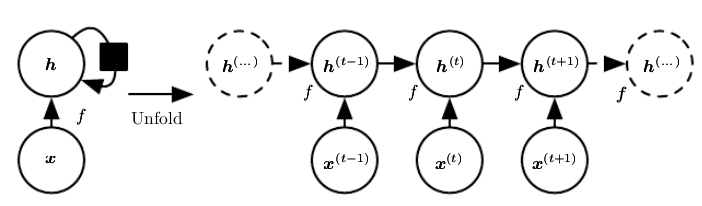
\includegraphics[height = 3cm, width = 10 cm]{img/grafo computacional 1.png}
                \caption{Una red recurrente sin salidas. Esta red solo procesa la información desde la entrada $x$ incorporándola al estado $h$ que se transmite hacia adelante a través del tiempo. (Izquierda) Diagrama del circuito, el cuadrado negro indica un retraso de un solo paso de tiempo. (Derecha) La misma red vista como un grafo desplegado, ahora cada nodo se asocia a una instancia temporal concreta. }
                \label{fig:grafo 1}
        \end{figure}
        
        
    Cuando se entrena a la red para realizar una predicción futura a partir del pasado, la red aprende a usar $h^{(t)}$ como una especia de resumen (con pérdidas) de los aspectos relevantes de la secuencia pasada de las entradas hasta el tiempo $t$. El resumen tiene pérdidas, ya que asigna una secuencia de longitud arbitraria, $x^{(t)},x^{(t-1)},...,x^{(2)},x^{(1)}$ a un vector de longitud fija $h^{(t)}$. Dependiendo del criterio de entrenamiento, este resumen podría conservar unos aspectos de la secuencia con más precisión que otros. \\
        
    La ecuación \ref{eq:rnn} puede dibujarse de dos maneras distintas. La primera es un diagrama que contiene un nodo para cada componente. Desde este punto de vista, la red define un circuito que funciona en tiempo real, con partes físicas cuyo estado actual puede influir en su estado futuro como en la izquierda de la figura \ref{fig:grafo 1}. El cuadrado negro se usa para indicar que la interacción tiene lugar con un retraso de un paso de tiempo, desde el estado en el tiempo $t$ al estado en el tiempo $t+1$. La segunda manera es desplegar el grafo, ahora cada componente está representada por muchas variables diferentes, con una variable por paso de tiempo que representa el estado de la componente en ese momento. Cada variable para cada paso de tiempo se dibuja como un nodo separado, como en la derecha de la figura \ref{fig:grafo 1}. \\ 
        
        
        
%%%%%%%%%%%%%%%%%%%%%%%%%%%%%%%%%%%%%%%%%%%%%%%%%%%%%%%%%%%%%%%%%%%%%%%%%%%%%%%%%%%%%
%%%%%%%%%%%%%%%%%%%%%%%%%%%%%%%%%%%%%%%%%%%%%%%%%%%%%%%%%%%%%%%%%%%%%%%%%%%%%%%%%%%%%
%%%%%%%%%%%%%%%%%%%%%%%%%%%%%%%%%%%%%%%%%%%%%%%%%%%%%%%%%%%%%%%%%%%%%%%%%%%%%%%%%%%%%


    \section{Funcionamiento de RNNs}
        
    La estructura y el proceso de despliegue de las RNNs introducen dos grandes ventajas: La primera es que independientemente de la longitud de la secuencia, el modelo aprendido siempre tiene el mismo tamaño de entrada porque la entrada se especifica en términos de la transición de un estado a otro en vez de estar especificada en términos una longitud variable de estados. La segunda es que es posible usar la misma función de transición $f$ con los mismos parámetros en cada paso de tiempo. Estos dos factores hacen posible el aprendizaje de un único modelo $f$ que opera en todos los pasos de tiempo y todas las longitudes de secuencia, en lugar de tener que aprender un modelo separado $g$ para todos los pasos de tiempo posibles. El aprendizaje de un único modelo compartido permite la generalización a longitudes de secuencia que no aparecen en el conjunto de entrenamiento y que permite que el modelo sea estimado con muchos menos ejemplos de entrenamiento de los que necesitaría en caso de que no se compartieran los parámetros. \\
        
    De acuerdo a lo anterior, se pueden diseñar una amplia variedad de RNNs. Algunos patrones de diseño importantes son los siguientes: 
        
            \begin{itemize}
                \item Redes recurrentes que producen una salida en cada paso de tiempo y tienen conexiones recurrentes entre las unidades ocultas. (Fig. \ref{grafo:rnn2})
                
                \item Redes recurrentes que producen una salida en cada paso de tiempo y tienen conexiones recurrentes sólo desde la salida en un paso de tiempo a las unidades ocultas en el siguiente paso de tiempo. (Fig. \ref{fig:rnn2tipo})
                
                \item Redes recurrentes con conexiones recurrentes entre las unidades ocultas que leen una secuencia completa y luego producen una única salida. (Fig. \ref{fig:rnn3tipo})
            \end{itemize}
            
        Vamos a explicar el funcionamiento de la RNNs de la figura \ref{grafo:rnn2} por ser bastante representativo. En dicha figura tenemos un grafo computacional que calcula la pérdida en el entrenamiento de una de una red recurrente que asigna una secuencia de entrada de valores $x$ a una secuencia de valores de salida $o$. Una pérdida $L$ mide lo lejos que está $o$ de la etiqueta del ejemplo de entrenamiento $y$. Cuando se usan las softmax como salidas suponemos que $o$ es un logaritmo de probabilidades y que no está normalizado. Entonces, $L$ internamente calcula $\hat{y} = softmax(o)$ y lo compara con $y$. La RNN tiene entradas a conexiones ocultas parametrizadas por una matriz de pesos $U$, conexiones recurrentes de unidades ocultas a unidades ocultas parametrizadas por una matriz de pesos $W$ y conexiones de unidades ocultas a salidas parametrizadas por una matriz de pesos $V$. \\
            
            
            \begin{figure}[ht]
                \centering
                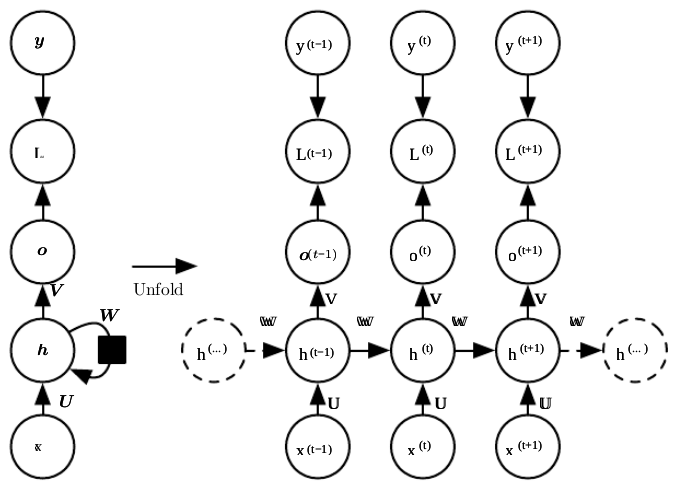
\includegraphics[scale=0.5]{img/grafo 2.png}
                \caption{Un grafo computacional que representa una RNN que produce una salida en cada paso de tiempo y tiene conexiones recurrentes entre las unidades ocultas. (Izquierda) la RNN y su pérdida dibujadas por conexiones recurrentes. (Derecha) Lo mismo pero visto como un grafo computacional desplegado donde cada nodo está asociado a un determinado paso de tiempo. }
                \label{grafo:rnn2}
            \end{figure}
            
        Desarrollamos las ecuaciones de la propagación hacia adelante para la RNN de la figura \ref{grafo:rnn2}. Como no se especifica la función de activación para las unidades ocultas vamos a suponer la tangente hiperbólica. Tampoco se especifica la forma exacta de la función de salida y pérdida, por lo que supondremos que la salida es discreta. Una forma natural para representar variables discretas es considerar la salida $o$ como si dieras las probabilidades logarítmicas sin normalizar de cada valor posible de la variable discreta. A continuación, podemos aplicar la operación softmax para obtener un vector $\hat{y}$ de probabilidades normalizadas sobre la salida. La propagación hacia adelante comienza en el estado inicial $h^{(0)}$. Luego para $t=1,...,\tau$ aplicamos las siguientes ecuaciones: 
        
            \begin{align}
                a^{(t)} &= b + Wh^{(t-1)} + Ux^{(t)},\\
                h^{(t)} &= \tanh{(a^{(t)})}, \\
                o^{(t)} &= c + Vh^{(t)}, \\
                \hat{y}^{(t)} &= softmax(o^{(t)})
            \end{align}
                

        \noindent donde los parámetros son los vectores de sesgo $b$ y $c$ junto con las matrices de pesos $U, V$ y $W$ para las conexiones de entrada a una unidad oculta, de una unidad oculta a uno de salida y de una unidad oculta otra oculta, respectivamente. Esto es un ejemplo de una red recurrente que asigna una secuencia de entrada a una secuencia de salida de la misma longitud. La pérdida total para una secuencia de valores $x$ y otra secuencia de valores $y$ sería sólo la suma de las pérdidas en todos los pasos de tiempo. Por ejemplo, si $L^{(t)}$ es la función de verosimilitud logarítmica negativa de $y^{(t)}$ dado $x^{(1)},...,x^{(t)}$, entonces
        
            \begin{align}
               L \big( \{x^{(1)},...,x^{(\tau)}\},\{y^{(1)},...,y^{(\tau)}\} \big) &= \sum_{t} L^{(t)}, \\
                &= -\sum_{t} \log p_{model} \big( y^{(t)} | \{x^{(1)},...,x^{(t)}\} \big)
            \end{align}  
        
        \noindent donde $p_{model} \big( y^{(t)} | \{x^{(1)},...,x^{(t)}\} \big)$ viene dado por la lectura de la entrada de $y^{(t)}$ del vector de salida del modelo  $\hat{y}^{(t)}$. El cálculo del gradiente de esta función de pérdida con respecto a los parámetros es una operación costosa ya que implica moverse de izquierda a derecha a través del grafo seguida de la propagación para atrás que va de derecha a izquierda. Tampoco se puede paralelizar (en el caso que estamos tratando, en otras RNNs, si se puede) ya que se realiza de manera secuencial por necesitar cada estado información del anterior. Tanto el tiempo de ejecución como el coste en memoria son $O(\tau)$. El algoritmo de backpropagation que se aplica en este tipo de redes neuronales se conoce como \textit{back-propagation a través del tiempo} (BBTT)\\ 
        
        \begin{figure}[htpb]
            \centering
            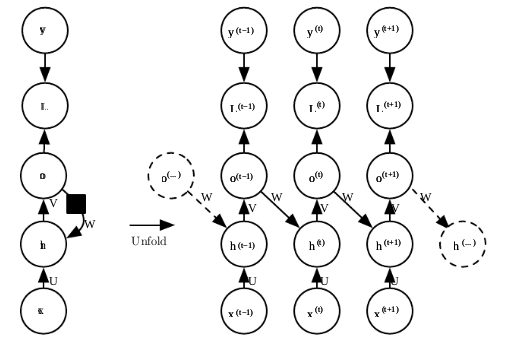
\includegraphics[scale=0.5]{img/rnn tipo.png}
            \caption{RNN cuya única recurrencia es la conexión de retroalimentación desde la salida a la capa oculta}
            \label{fig:rnn2tipo}
        \end{figure}
        
        
        
        \begin{figure}[htpb]
            \centering
            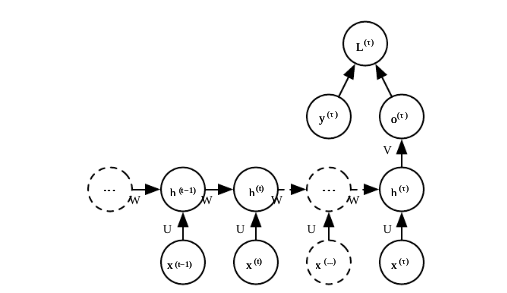
\includegraphics[scale=0.5]{img/rnn tercer tipo.png}
            \caption{Grafo desplecado de una RNN con una única salida al final de la secuencia. Esta red se suele usar para resumir una secuencia y producir una representación de tamaño fijo utilizada como entrada para el procesamiento posterior}
            \label{fig:rnn3tipo}
        \end{figure}
        
        
        
\section{Redes Neuronales Recursivas}

    Las redes neuronales recursivas representan una generalización de las redes recurrentes, con un tipo diferente de gráfico computacional que se estructura como un árbol profundo en lugar de la estructura de cadena de las RNNs. Un ejemplo típico es el de la figura \ref{fig:reNN}. Estas redes se introdujeron por primera vez en torno a 1990 y se suelen aplicar debido a su éxito en procesamiento de lenguaje natura y visión por computador entre otras disciplinas. Una cuestión que hay que pensar al usar estas redes es como estructurar el árbol. \\
        
    Una clara ventaja de estas redes sobre las recurrentes es que para una secuencia de la misma longitud $\tau$, la profundidad medida como el número de composiciones de operaciones no lineales puede ser drásticamente reducida de $\tau$ a $O(\log \tau)$, lo que ayuda a tratar las dependencias a largo plazo. \\
        
    Una cuestión abierta hoy en día es como estructurar de la mejor manera el árbol. Una propuesta es que se estructure de tal manera que no dependa de los datos, como un árbol binario equilibrado. Aunque la respuesta a esta cuestión puede ser tratada de diferentes maneras dependiendo del problema.
        
        \begin{figure}[htpb]
                \centering
                \includegraphics[scale=0.5]{recursivenn.png}
                \caption{La figura muestra un caso de aprendizaje supervisado en el que se proprociona un objetivo y se asocia a toda la secuencia. Una red recursiva tiene un grafo computacional que generaliza el de la red recurrente de una cadena a un árbol. Una secuencia de longitud variable $x^{(1)},...,x^{(t)}$ puede ser mapeada a una representación de tamaño fijo (la salida $o$) con un conjunto fijo de parámetros (matrices U, V y W) }
                \label{fig:reNN}
        \end{figure}
        
        
\section{El problema de la dependencias a largo plazo}\label{seccion:sorpresa}

    Una de las principales características de las redes neuronales recurrentes es que pueden conecta la información anterior con la actual, por lo que no resulta descabellado pensar que pueden recordar aspectos del pasado. Sin embargo, ¿Esto es así del todo?\\
    
    A veces, solo necesitamos mirar la información reciente para realizar la tarea actual como el ejemplo que se expuso al principio del capítulo sobre el \textit{Kilimanjaro}. En estos casos en los que la distancia entre la información relevante y el lugar en el que debe ser usada sea reducida, las RNNs pueden usar correctamente la información anterior que tienen. \\
    
    El otro extremo son los casos en los que necesitemos más contexto, es decir, cuando la distancia entre la información relevante y el lugar en el que debe ser usada es bastante amplia. Supongamos un texto en el que al principio del mismo empiece con \textit{Me crié en Italia} y tras todo un párrafo al final aparezca \textit{hablo fluidamente el italiano}. Si nuestro objetivo es predecir la última palabra del párrafo, \textit{italiano}, necesitamos usar la información del principio y es posible que la brecha entre la información relevante y el punto en que se necesita sea demasiado grande. \\
    
    Desgraciadamente, a medida que esa brecha crece, las RNN se vuelven incapaces de aprender a conectar la información. En teoría las RNN son absolutamente capaces de manejar estas dependencias a largo plazo. Pero en la práctica no es del todo así. Este problema fue estudiado por \textit{Hochreiter (1991)} y Bengio, et al. (1994) \cite{schmidhuber1997long, pascanu2013difficulty} y encontraron algunas razones fundamentales por las que podría ser difícil. No vamos a entrar en detalle ni a explicarlo de manera rigurosa pero sí que vamos a comentar por encima la causa del problema. \\

\subsection{Causa: Desvanecimiento/Explosión del gradiente}


        Las redes neuronales, en particular las RNNs, con grafos computacionales muy profundos presentan una dificultad a la que se debe enfrentar el algoritmo de optimización. Al aplicarse la misma operación de manera repetida en cada paso de tiempo provoca lo que se conoce como desvanecimiento y explosión del gradiente. \\
        
        Vamos a explicarlo primero con un ejemplo y posteriormente extendemos la explicación al caso de las RNN. Supongamos que un grafo computacional tiene un camino que consiste en multiplicar repetidamente por una matriz de pesos $W$. Después de $t$ unidades de tiempo, sería equivalente a multiplicar por $W^t$. Supongamos que $W$ tiene una descomposición en valores propios de la forma $W=V\cdot diag(\lambda) \cdot V^{-1}$, por lo que 
        
        \begin{equation}
            W^t = (V\cdot diag(\lambda) \cdot V^{-1})^t = V\cdot diag(\lambda)^t \cdot V^{-1} 
        \end{equation}
        
        Entonces, cualquier valor propio $\lambda_i$ que no esté en valor absoluto cerca de $1$ puede explotar si es bastante mas grande que $1$ o puede desvanecerse si está próximo a $0$. El problema de los gradientes evanescentes o explosivos se refiere al hecho de que los gradientes de un gráfico de este tipo también se escalan según $diag(\lambda_i)$. Por una parte, los gradientes evanescentes hacen que sea dificil saber en qué dirección deben moverse los pesos para mejorar la función de coste. Por otra parte, los gradientes explosivos hacen que el aprendizaje sea inestable. Es más común que ocurra el desvanecimiento que la explosión\\
        
        El principal problema es que los gradientes propagados a lo largo de muchas etapas tienden a desaparecer o a explotar. Si asumimos que los parámetros son tales que la RNN es estable (no explotan) la dificultad con las dependencias a largo plazo surge de los pesos exponencialmente más pequeños dados por las interacciones a largo plazo (que implican la multiplicación de muchos jacobianos) en comparación con las de corto plazo.\\
        
        Las RNNs traen consigo la composición de la misma función varias veces, una vez por unidad de tiempo. Estas composiciones pueden llegar a originar un comportamiento exageradamente no lineal. Esta composición de funciones se asemeja un poco a la multiplicación de matrices. Podemos pensar en la relación de recurrencia 
        
        \begin{equation}
            h^{(t)} = W^T \cdot h^{(t-1)}
        \end{equation}
        
        \noindent como una RNN muy simple que carece de una función de activación no lineal y de entradas. La relación anterior se puede ver también de la forma 
        
        \begin{equation}
            h^{(t)} = (W^t)^T \cdot h^{(0)}
        \end{equation}
        
        \noindent por lo que si $W$ admitiera una descomposición en valores singulares de la forma 
        
        \begin{equation}
            W = Q \Lambda Q^T
        \end{equation}
        
        \noindent siendo $Q$ una matriz ortogonal, se tendría que 
        
        \begin{equation}
            h^{(t)} = Q^T \cdot \Lambda^t \cdot Q \cdot h^{(0)}
        \end{equation}
        
        \noindent Por lo que tendríamos una situación igual a la del primer ejemplo. Los valores propios están elevados a la potencia de $t$, causando una explosión si son bastante más grandes que uno y un desvanecimiento si están próximos cero. Este problema es particular de las RNNs. 


\section{Long short-term Memory y GRU}

    Tras entender el concepto de RNNs ahora presentamos aquellas que vamos a emplear en la prácticas, las cuales reciben el nombre de LSTM (\textit{long short-term memory)} y GRU (\textit{Gated Recurrent unit}) las cuales se presentaron como solución al problema de la explosión y desvanecimiento del gradiente. \\

    \subsection{LSTM}

    Las LSTM (\textit{long short-term memory)} son un tipo especial de RNN, capaces de aprender dependencias a largo plazo. Fueron presentadas por \textit{Hochreiter y Schimidhuber} (1997) \cite{hochreiter1997long} y refinadas posteriormente por la comunidad investigadora. Hoy en día son muy usadas en multitud de campos, el más destacado es el proceseamiento del lenguaje natural. \\
    
    Este tipo de RNN está especialmente diseñada para evitar la dependencia a largo plazo, por lo que recordar información durante largos períodos de tiempo es su especialidad. Se basan en la idea de crear caminos a través del tiempo entre las entradas, salidas y estados internos que permitan recordar información u olvidarla si ya no es útil. De este modo se consigue que tengan derivadas que no se desvanezcan ni exploten. El objetivo es permitir a la red que acumule información como por ejemplo, la evidencia de una característica o categoría particular durante un largo periodo de tiempo y una vez que dicha información guardada se haya usado se permita que pueda ser olvidada. El hecho de olvidar la información no ocurre por arte de magia, sino que la red debe de ser capaz de aprender cuándo hacerlo y cuándo no.  \\
        
    Todas las redes neuronales recurrentes tienen la forma de una cadena en la que se repiten módulos, en las RNNs  típicas, estos módulos constan de una estructura muy simple formada por una operación no lineal elemento a elemento de una transformación afín de la entrada y las unidades recurrentes (Fig. \ref{fig:celda RNN}). En cambio, las LSTM, aunque presenten también una cadena de celdas repetidas, estas celdas cuentan con una recurrencia interna (bucle interno) además de la recurrencia externa de la RNN y una estructura mucho más sofisticada con puertas de control que manejan el flujo de la información. Los bucles internos producen trayectorias en las que el gradiente puede fluir durante largos periodos de tiempo. Un aspecto clave es que el peso de estos bucles esté condicionado por el contexto en vez de ser fijo, haciendo que el peso del bucle propio esté controlado por una unidad oculta (Fig. \ref{fig:celda LSTM}).\\
    
    
    \begin{figure}[H]
        \centering
        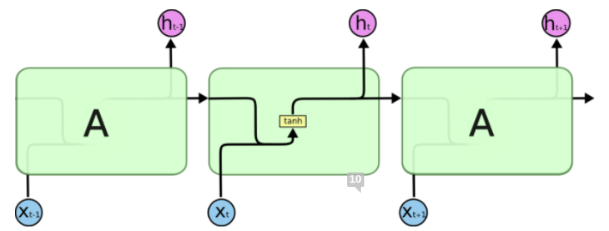
\includegraphics[scale=0.5]{rnng.png}
        \caption{Celda de una RNN común}
        \label{fig:celda RNN}
    \end{figure}
    
    \begin{figure}[H]
        \centering
        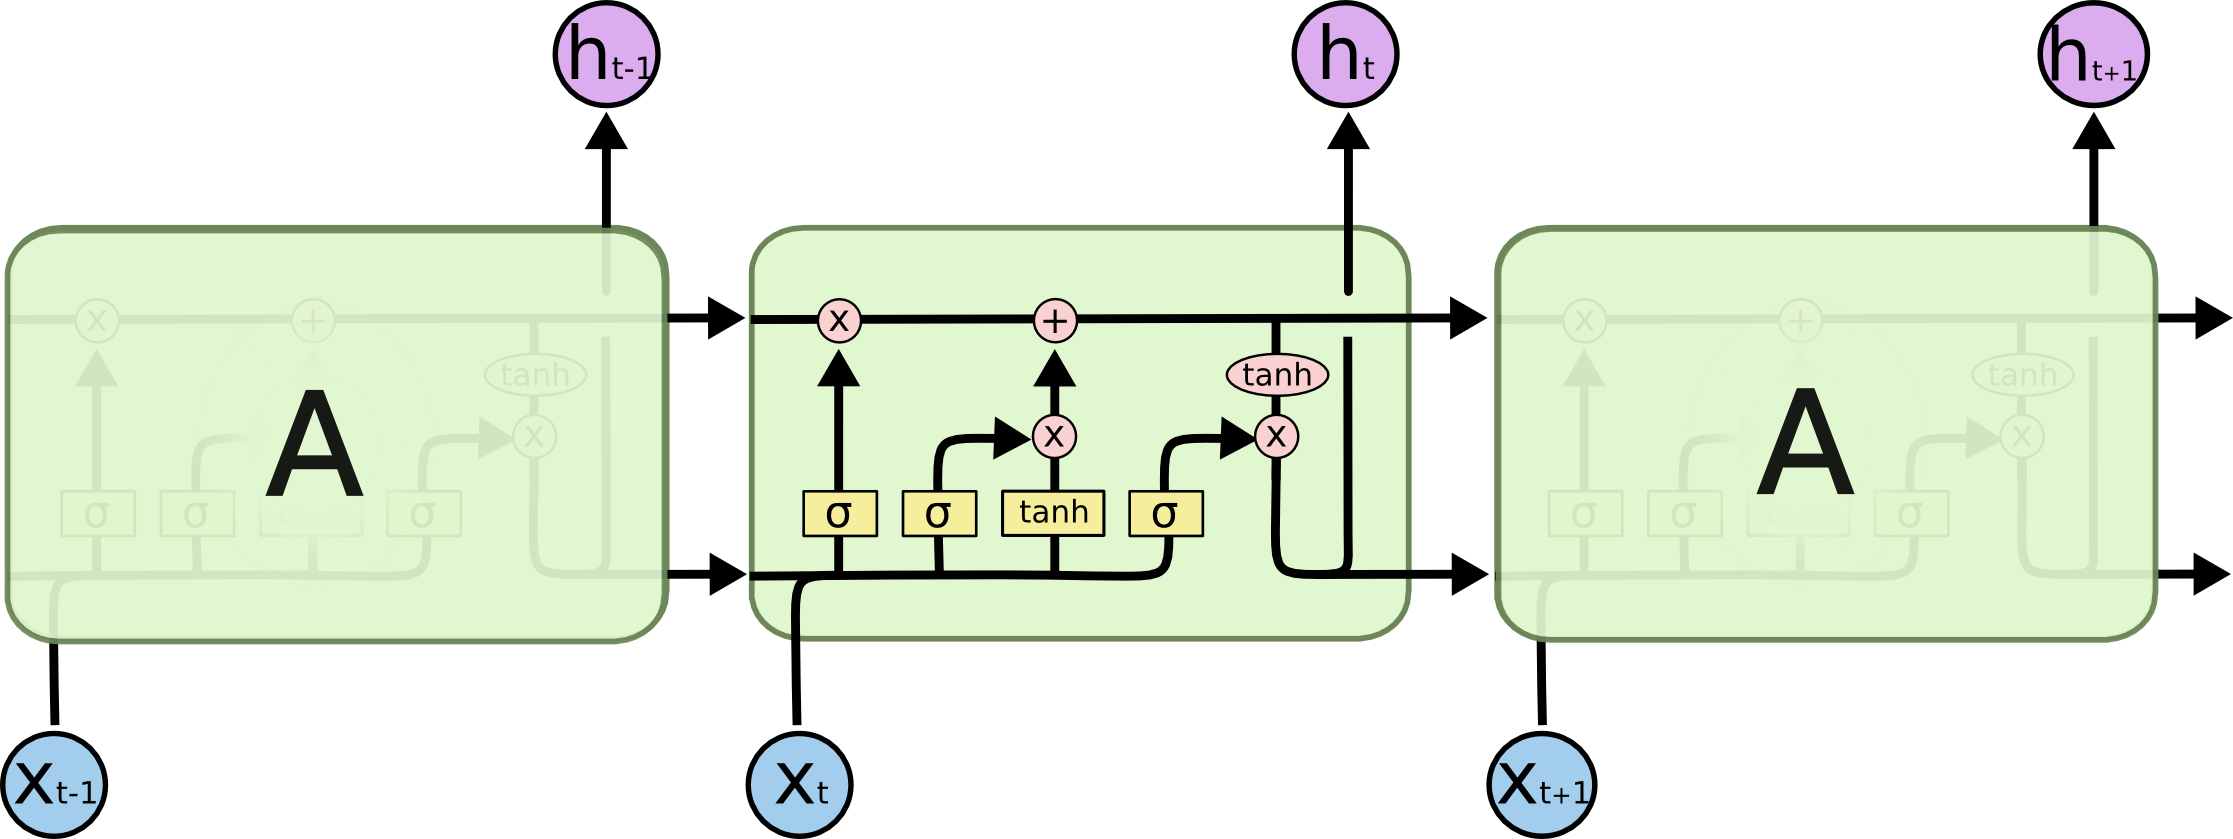
\includegraphics[scale=0.5]{lstmg.png}
        \caption{Celda de una LSTM. Podemos apreciar las dos recurrencias (interna y externa) y las puertas de control dentro de la celda}
        \label{fig:celda LSTM}
    \end{figure}
    
    De aquí en adelante usaremos diagramas para detallar el funcionamiento de una LSTM, por lo que usaremos la siguiente notación (Fig. \ref{fig:LSTM legend}) \\
    
    \begin{figure}[H]
        \centering
        \includegraphics[scale=0.7]{img/diagram legend.png}
        \caption{Notación para los diagramas.}
        \label{fig:LSTM legend}
    \end{figure}
    
    La clave de las LSTMs es el estado de la celda, que en un tiemop $(t)$ y una celda $i$, se representa por $C_i^{(t)}$ y viene dada por la línea horizontal que atraviesa la parte superior del diagrama \ref{fig:LSTM estado} y resaltada en negro. El estado de la celda consta de un bucle interno y es una especie de cinta transportadora. Corre en línea recta por toda la cadena con solo algunas transformaciones lineales menores. Es muy fácil que la información fluya a lo largo de ella sin cambios. \\
    
    	 \begin{figure}[H]
	        \centering
	        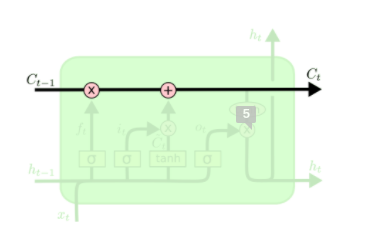
\includegraphics[scale=0.7]{d1.png}
	        \caption{Estado de una celda LSTM}
	        \label{fig:LSTM estado}
	    \end{figure}
	    
	 Como ya se comentó, las LSTMs tienen la habilidad de eliminar o añadir información al estado de la celda gracias a las puertas. Estas están compuestas por una función sigmoidal y una operación de multiplicación punto a punto. La función sigmoidal (Fig. \ref{fig:LSTM sigmoidal}), cuya salida está comprendida entre cero y uno viene a indicar cuánta información deja pasar. Un valor de cero significa que no deja nada pasar mientras que un valor de uno significa que lo deja todo. Una celda LSTM tiene tres puertas de este tipo para proteger y controlar el estado de la celda. \\ 
	 
	 \begin{figure}[H]
	     \centering
	     \includegraphics[scale=0.8]{img/LSTM sigmoidal.png}
	     \caption{Capa Sigmoidal. Esta capa controla la cantidad de información que se deja pasar.}
	     \label{fig:LSTM sigmoidal}
	 \end{figure}
	    
	     
	 El primer paso es decidir que información vamos olvidar del estado de la celda empleando para ello la puerta de olvido (Fig. \ref{fig:dd2}). Los pesos del bucle interno son controlados por esta puerta que recibe como entrada los vectores $x^{(t)}$ y $h^{(t-1)}$ que contienen los inputs de entrada y la información de las celdas anteriores. Devuelve un vector conteniendo números entre $0$ y $1$ al estado $C_{t-1}$ para decidir qué olvidar, qué no olvidar y cúanto olvidar. \\
	    
	    
	    \begin{figure}[H]
	      \centering
	      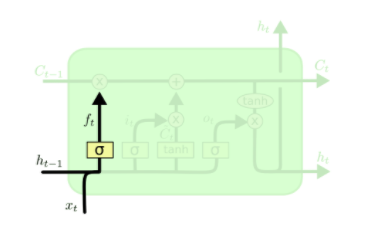
\includegraphics[scale=0.7]{dd2.png}
	      \caption{Puerta de olvido}
	      \label{fig:dd2}
	    \end{figure}
	    
	 La puerta de olvido para un instante de tiempo $(t)$ y una celda $i$ la vamos a modelar por la función $f_i^{(t)}$ cuya expresión viene dada por
	 
	 \begin{equation}\label{eq:lstm_f}
	     f^{(t)}_i = \sigma \Big( b^f_i + \sum_j U_{i,j}^f x^{(t)}_j + \sum_j W_{i,j}^f h^{(t-1)}_j \Big)
	 \end{equation}
	    
	\noindent donde $b_i^f, U_i^f$ y $W_i^f$ son respectivamente el sesgo, los pesos de entrada y los pesos recurrentes para la puerta de olvido en la celda $i$. A modo de ejemplo, imaginemos que tenemos un modelo de un lenguage el cual intenta predecir la siguiente palabras basándose en las anteriores. En este problema la celda de estado puede tener codificado el género del sujeto o la persona, entonces un cambio del mismo supondría la necesidad de eliminar la información del sujeto anterior anterior así como por ejemplo, determinantes, conjugaciones verbales o pronombres. Es en este punto donde decidimos olvidar toda esa información. \\
	  
    El siguiente paso es decidir qué información vamos a almacenar en el estado de la celda, esto se hace en dos fases. La primera es decidir qué valores se van a actualizar usando una función sigmoidal conocida como la \textit{puerta de entrada} (Fig. \ref{fig:LSTM input gate}), $g_i^{(t)}$. Después, una capa $\tilde{C}_t$, con una función $tanh$ (también puede ser una función sigmoidal) crea un vector con posibles candidatos a ser añadidos. En el ejemplo, es en este punto donde nos gustaría añadir el género del nuevo sujeto al estado de la celda para reemplazar el antiguo que estamos olvidando. Las expresiones vienen dadas por
    
    \begin{equation}
    \begin{aligned}
        g^{(t)}_i & = \sigma \Big( b^g_i + \sum_j U_{i,j}^g x^{(t)}_j + \sum_j W_{i,j}^g h^{(t-1)}_j \Big) \\
        \tilde{C}^{(t)} & = \tanh \Big( b^C_i + \sum_j U^C_{i,j}x^{(t)}_j + \sum_j W^C_{i,j} h^{(t-1)}_j \Big)
    \end{aligned}
    \end{equation}
    
    
    \noindent donde $b^g, b^C, U^g, U^C, W^g, W^C$ son los sesgos, los pesos de entrada y los pesos recurrentes asociados a la puerta de entrada y la función que establece los candidatos respectivamente. \\
	    
    

	    \begin{figure}[H]
	      \centering
	      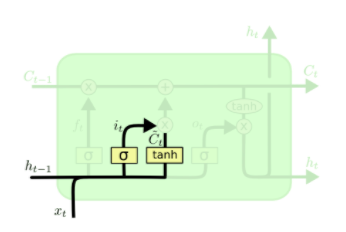
\includegraphics[scale=0.7]{dd3.png}
	      \caption{Puerta de entrada. En este diagrama la función $g^{(t)}$ viene representada por }
	      \label{fig:LSTM input gate}
	    \end{figure}
	  
	 \noindent En la segunda fase se combinan la salida de la puerta de entrada y este nuevo vector de candidatos para actualizar el estado antiguo al estado nuevo (Fig. \ref{fig:LSTM update}). Los pasos anteriores ya decidieron que información usar para ello, por tanto solo queda multiplicar el antiguo estado por la salida de la puerta de olvido y sumarlo a la multiplicación de la salida de la puerta de entrada con el vector de candidatos creado por la función $\tilde{C}^{(t)}$. Para el ejemplo del modelo de lenguaje, aquí es donde dejaríamos la información sobre el género del sujeto anterior y añadiríamos la nueva información. 
	 
	 
	   \begin{figure}[H]
	      \centering
	      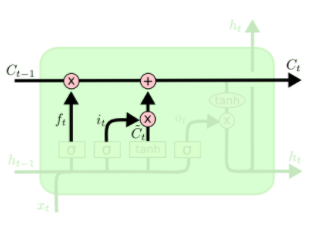
\includegraphics[scale=0.5]{dd5.png}
	      \caption{Actualización}
	      \label{fig:LSTM update}
	   \end{figure}	  

    \begin{equation}
	     C^{(t)}_i = f^{(t)}_i * C^{(t-1)}_i + g^{(t)}_i * \tilde{C}_i^{(t)}
	 \end{equation}

    Por último, se decide qué o cuánta información va a ser sacada como salida de la capa oculta, la cual se representa por $h_i^{(t)}$ y se le conoce puerta de salida (Fig. \ref{fig:LSTM output gate}). Primero se aplica una función sigmoidal que decide qué partes del estado van a ser usadas para la salida. Tras ello, se aplica una función $tanh$ (que mapea los valores entre $-1$ y $1$) al estado actual y se multiplica por la salida de la sigmoidal. 
    
    \begin{equation}
    \begin{aligned}
        o^{(t)}_i & = \sigma \Big( b^o_i + \sum_j U^o_{i,j} x^{(t)}_j + \sum_j W^o_{i,j} h^{(t-1)}_j \Big) \\
        h^{(t)}_i & = tanh \big( C^{(t)}_i \big) * o^{(t)}_i
    \end{aligned}
    \end{equation}

    \noindent donde los parámetros $b^o, W^o$ y $U^o$ son los sesgos, los pesos de entrada y los pesos recursivos respectivamente. En el ejemplo del modelo de lenguaje, si nos topamos con un nuevo sujeto, podríamos querer emitir información relevante para el verbo, como por ejemplo, decir si el sujeto está en singular o plural para obtener información sobre la conjugación del verbo. 

	   \begin{figure}[H]
	      \centering
	      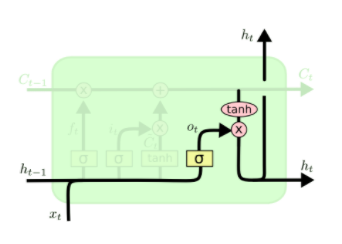
\includegraphics[scale=0.5]{dd6.png}
	      \caption{Puerta de salida}
	      \label{fig:LSTM output gate}
	   \end{figure}
    

    \subsubsection{Variantes}
    

    El ejemplo anterior es de una arquitectura en concreto, de hecho, la mayoría de LSTMs usadas son variaciones de esta última. Por ejemplo, en la imágenes \ref{fig:lstm_v1} y \ref{fig:lstm_v2} tenemos dos variantes. 
	   
	   \begin{figure}[H]
	       \centering
	       \includegraphics[scale=0.5]{dd7.png}
	       \caption{Variación 1: Se introducen \textit{peephole connections} permitiendo que las puertas de olvido y salida puedan consultar el estado. Hay otras muchas variantes de este modelo en función de que puertas tengan las \textit{peephole connections.}}
	       \label{fig:lstm_v1}
	   \end{figure}
	   
	   
	   \begin{figure}[H]
	       \centering
	       \includegraphics[scale=0.5]{dd8.png}
	       \caption{Variación 2: En esta arquitectura en vez de decidir de manera separada que información vamos a olvidar y a añadir, se toma la decisión de forma conjunta.}
	       \label{fig:lstm_v2}
	   \end{figure}
	    
	    
    \subsection{GRU}
    
        Las GRU (Fig. \ref{fig:gru}) \cite{chung2014empirical} son otro tipo de redes neuronales recurrentes, o incluso también pueden ser vistas como una variante de las LSTM cuya principal diferencia radica en que éstas usan una puerta que controla simultáneamente la parte que olvida y la parte que actualiza. Al igual que las LSTMs, las GRUs cuentan con una gran cantidad de variaciones. Su expresión viene por  \\
        
        \begin{equation}
            h^{(t)} = u^{(t-1)}_i h^{(t-1)}_i + ( 1 - u^{(t-1)}_i) \sigma \Big( b_i + \sum_j U_{i,j} x^{(t)}_j + \sum_j W_{i,j} r^{(t-1)}_j h^{(t-1)}_j \Big),
        \end{equation}
        
        \noindent donde $u$ representa la puerta de actualización y $r$ la de reinicio y cuyas ecuaciones son, 
        
        \begin{equation}
            u^{(t)}_i = \sigma \Big( b^u_i + \sum_j U^n_{i,j} x^{(t)}_j + \sum_j W^u_{i,j}h^{(t)}_j\Big)
        \end{equation}
	    
	    \begin{equation}
	        r^{(t)}_i = \sigma \Big( b^r_i +  \sum_j U^r_{i,j} x^{(t)} + \sum_j W^u_{i,j}h^{(t)}_j \Big)
	    \end{equation}
	    
	    
	    \begin{figure}[H]
	      \centering
	      \includegraphics[scale=0.6]{dd9.png}
	      \caption{Ejemplo de un arquitectura de GRU. En este ejemplo podemos ver apreciar como se juntan la puerta de olvido y actualización en una. También se aprecia la fusión del estado de la celda con el estado de la unidad oculta. Este modelo se está convirtiendo cada vez más popular.}
	      \label{fig:gru}
	    \end{figure}
	    
	   

    


\endinput


\setpartpreamble[c][0.75\linewidth]{%
	\bigskip % Deja un espacio vertical en la parte superior
 El propósito de este capítulo es enfrentarse al problema de clasificación de señales de ECG. Para ello se partirá del conocimiento adquirido en las dos partes anteriores y se desarrollarán un conjunto de modelos para resolver este problema. Además se estudiarán otras propuestas ya existentes y se realizará una comparación con los modelos propuestos.
}
\cleardoublepage\part{Clasificación de Arritmias}
% !TeX root = ../libro.tex
% !TeX encoding = utf8



\setchapterpreamble[c][0.75\linewidth]{%
	\sffamily
  
      El objetivo de este capítulo es motivar e introducir al lector en el problema, para ello se abordará el asunto desde un aspecto descriptivo. Primeramente se realizará una descripción del problema, exponiendo la necesidad e importancia de enfrentar este tipo de problemas. Después, se presentará una sección que explica los electrocardiogramas para que de este modo el lector adquiera un mayor conocimiento del tema y le resulten familiares en lo que sigue. Posteriormente se hablará de la base de datos usada así como del principal inconveniente que presenta. Finalmente se incluirá un estado del arte en el que el lector podrá ponerse en contexto en cuanto al avance de este campo.

	\par\bigskip
}

\chapter{Descripción del problema}\label{ch:descripcion_problema}

\section{Descripción del problema}

    La fibrilación auricular es un ritmo cardíaco irregular y a menudo muy rápido (arritmia) que puede provocar coágulos de sangre en el corazón. Tener una fibrilación auricular incrementa la probabilidad de sufrir un accidente cerebrovascular, insuficiencia cardíaca y otras muchas complicaciones relacionadas con el corazón. Es una enfermedad que afecta a millones de personas en todo mundo y no entiende de género y edades. Sí es cierto que es más frecuente en personas de edad avanzada, pero en los últimos años se han incorporado muchos casos en jóvenes y adultos. Por este motivo, es de vital importancia poner las tecnologías más avanzadas en este área con objeto de salvar todas las vidas que se puedan y mejorar la calidad de las mismas. \\
    
    Se nos presenta un problema de clasificación de señales obtenidas por electrocardiogramas (ECG). El principal objetivo es discernir entre ritmos normales, es decir, aquellos ritmos propios de una persona sin patologías cardíacas y entre fibrilaciones auriculares (FA). No obstante, existen otras enfermedades parecidas a la fibrilación auricular, por este motivo, también es de vital importancia discernir entre estas otras enfermedades y la FA, ya que los tratamientos a seguir no van a ser iguales en caso de tener un tipo de enfermedad u otra. \\
    
    Para enfrentarnos al problema se ha recurrido a uno de los paradigmas dentro la inteligencia artificial que abordan este asunto de forma novedosa, el aprendizaje profundo. Este paradigma presenta una gran ventaja frente a los tradicionales, y es la ausencia a priori de conocimiento experto del tema, haciendo que cualquier persona pueda emprender el desarrollo de un problema de este tipo sin la necesidad de ser un experto en el tema. \\ 
    


\section{Electrocardiogramas}
    
    
    Un electrocardiograma, abreviado como ECG es un procedimiento médico indoloro, no invasivo y simple que registra la actividad eléctrica del corazón. Los latidos del corazón son posibles gracias a una pequeña señal eléctrica que circula por este órgano y es la responsable de guiar las contracciones y expansiones de las cavidades que lo forman. Un ECG muestra si su corazón está latiendo a un ritmo y con una fuerza normal, suponiendo un problema para la salud en caso contrario. Dicho en otras palabras, el ECG representa de manera visual la actividad eléctrica del corazón en función del tiempo, obtenida desde la superficie corporal del pecho. \\
    
    
    El ECG se usa para encontrar y vigilar varias enfermedades del corazón tales como obstrucción de arterias, insuficiencia cardíaca, arritmias (latidos cardíacos irregulares), ataques del corazón, obstrucción de arterias entre otras. \\
    
    Las partes de un ECG las podemos encontrar en la imagen \ref{fig:ECG}. Un ECG corriente que registra un latido cardíaco normal consta de una onda P, un complejo QRS, y una onda T. Generalmente, la onda U suele ser invisible. Estos fenómenos eléctricos no han de confundirse con los fenómenos mecánicos de contracción y relajación de las cavidades del corazón. La contracción del ventrículo, a lo cual nos referiremos a partir de ahora como sístole mecánica, comienza justo después del inicio del complejo QRS y termina justo antes del finalizar la onda T. La diástole, que es cuando la ventrículo se relaja y se rellena comienza justo después de que acabe la sístole correspondiente a la contracción de las aurículas, justo después de comenzar la onda P. \\
    
    La onda P es la señal que corresponde a la despolarización auricular. Esta onda es la responsable de provocar la contracción de las aurículas. El compejo QRS corresponde a la señal de despolarización ventricular e indica el inicio de la contracción de la ventrícula. Este complejo está formado por tres ondas, la Q, la R y la S. La onda Q es una onda negativa y representa una pequeña desviación previa a la sístole ventricular, la onda R es la primera deflexión positiva del complejo QRS y es la de mayor tamaño, es la responsable de la contracción de los ventrículos y finalmente, la onda S, es cualquier onda negativa que siga a la onda R. La onda T representa la relajación por parte de los ventrículos. Estas ondas aparecen una vez por cada pulso del corazón y cuando nos tomamos el pulso contamos el número de veces que se repite la onda R por intervalo de tiempo. Cualquier irregularidad en algunas de estas ondas puede dar lugar a enfermedades coronarias. \\
    
    \begin{figure}[H]
        \centering
        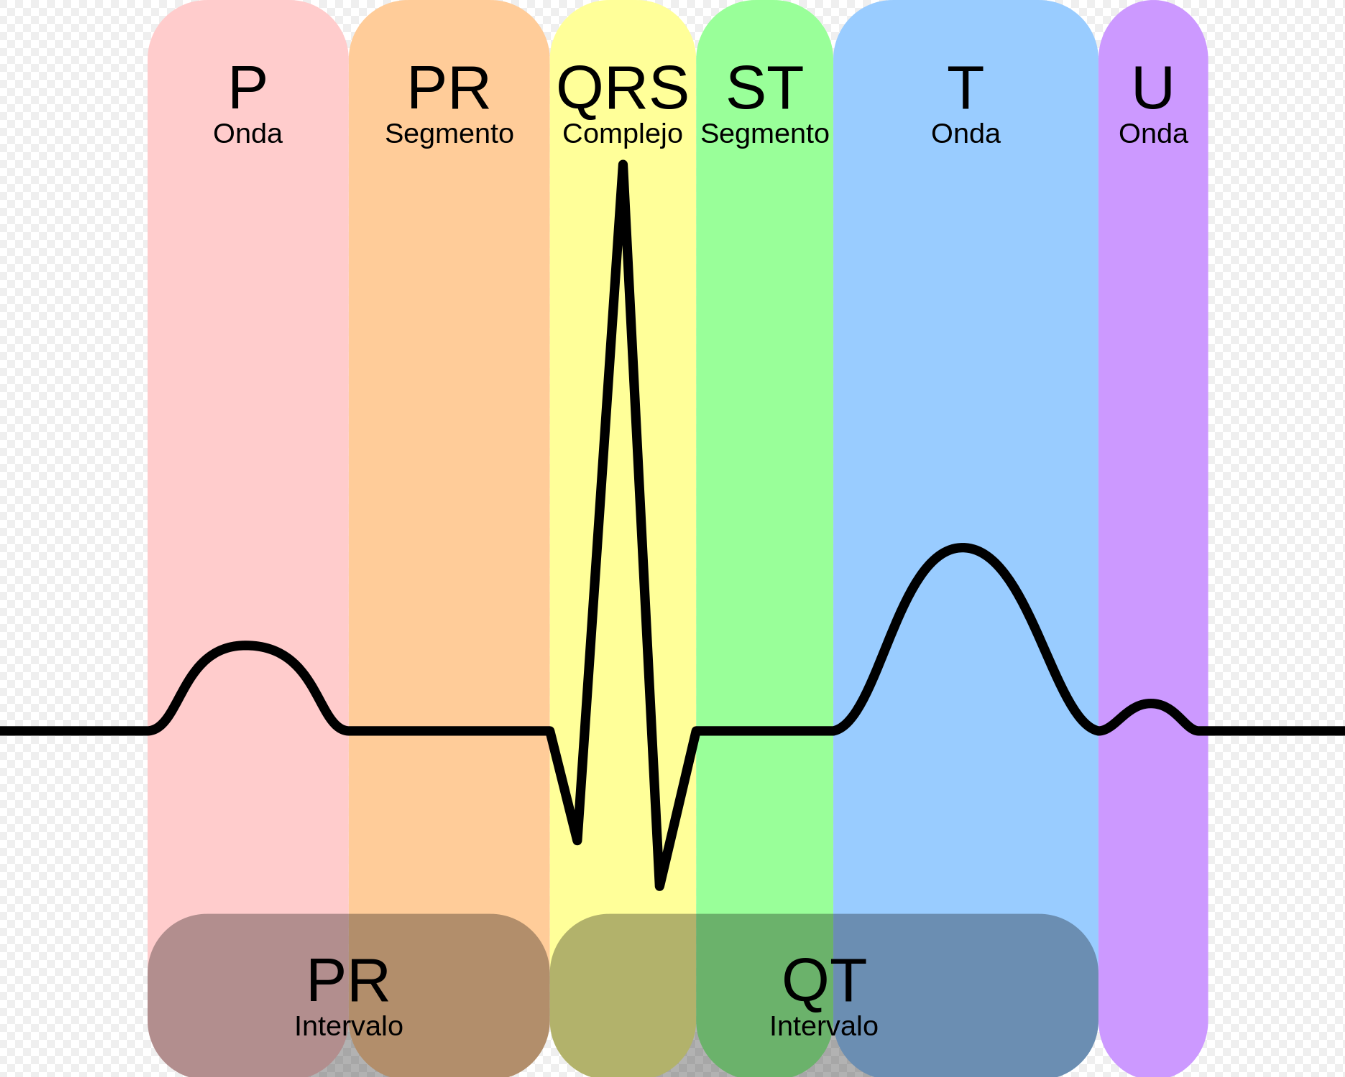
\includegraphics[height=5cm, width = 7cm]{img/ECG_2.png}
        \caption{Representación de un ECG normal distinguiendo por intervalos las distintas partes.\href{https://upload.wikimedia.org/wikipedia/commons/thumb/e/e8/EKG_Complex_es.svg/1280px-EKG_Complex_es.svg.png}{Fuente}}
        \label{fig:ECG}
    \end{figure}
    
    
    
    

\section{Base de Datos Experimental}

    Vamos a trabajar con una base de datos propuesta para una competición en el año 2017 por la plataforma \textit{PhysioNet/CinC} llamada \textit{AF Classification from a Short Single Lead ECG Recording: The PhysioNet/Computing in Cardiology Challenge 2017} y disponible a través de este a través de este \href{https://physionet.org/content/challenge-2017/1.0.0/}{enlace}. El objetivo de esta competición es fomentar el desarrollo de algoritmos que permitan clasificar, a partir de un único registro de derivación de ECG corto (entre 30 y 60 segundos), si el registro muestra un ritmo sinusal normal, una fibración auricular (FA), un ritmo alternativo o es demasiado ruidoso como para ser clasificado. \\
    
    Se define la FA como una \textit{taquiarritmia caracterizada por una activación auricular predominantemente descoordinada con el consiguiente deterioro de la función mecánica auricular}. La AF es la arritmia cardiaca sostenida más frecuente, que se presenta en el 1-2\% de la población general y viene asociada a una alta mortandad y morbilidad por la asociación de riesgo de muerte, ictus, hospitalización, insuficiencia cardiaca, etc. Aproximadamente más de 12 millones de personas de Europa y América padecen FA y su prevalencia se estima que será del triple de aquí a 30-50 años. Otro dato a tener en cuenta, es que la incidencia de la FA aumenta con la edad, desde menos del 0,5\% a los 40-50 años, hasta el 5-15\% en personas de 80 años. \\
    

    La detección de la FA es bastante compleja, ya que puede ser episódica. Los detectores de FA pueden considerarse pertenecientes a dos categorías: métodos basados en el análisis de la actividad auricular o en el análisis de la respuesta ventricular. Los primeros se basan en el análisis de la ausencia de ondas $P$ o la presencia de ondas $f$ fibrilatorias en el intervalo $TQ$. Estos métodos son muy sensibles a la contaminación, pero presentan la ventaja de ser bastante precisos si las señales están poco contaminadas y tienen una alta resolución. El segundo se basa en la predictibilidad del tiempo entre latidos (intervalos RR) de los complejos QRS en el ECG. Los intervalos RR se derivan de la característica de gran amplitud más obvia del ECG, el pico R, cuya detección puede ser mucho más resistente al ruido y por ello, se suele usar para detección automática de FA en tiempo real. \\

        Los estudios anteriores relativos a la clasificación de la FA suelen tener una aplicabilidad limitada ya que
        \begin{itemize}
            \item Solo se realizó la clasificación de los ritmos normales y de la FA
            \item El buen rendimiento se demostró en datos cuidadosamente seleccionados y a menudo limpios
            \item No se utilizó un conjunto de datos de prueba fuera de la muestra
            \item Sólo se utilizó un pequeño número de pacientes
        \end{itemize}

    
        
    Es bastante complejo detectar la FA de manera suficientemente fiable a partir de una sola derivación corta del ECG. Además, la amplia variedad de ritmos existentes tampoco facilita nada las cosas. En particular, hay muchos ritmos que no son FA y presentan intervalos RR irregulares que pueden ser similares a la FA. En este desafío, tratamos todos los ritmos anormales no relacionados con la FA como una sola clase y clasificamos los ritmos como: \\
        
        \begin{itemize}
            \item Ritmo sinusal normal (Paciente Sano)
            \item FA (Fibrilación auricular)
            \item Otro Ritmo
            \item Electrocardiogramas ruidosos
        \end{itemize}
        
        \begin{figure}[H]
            \centering
            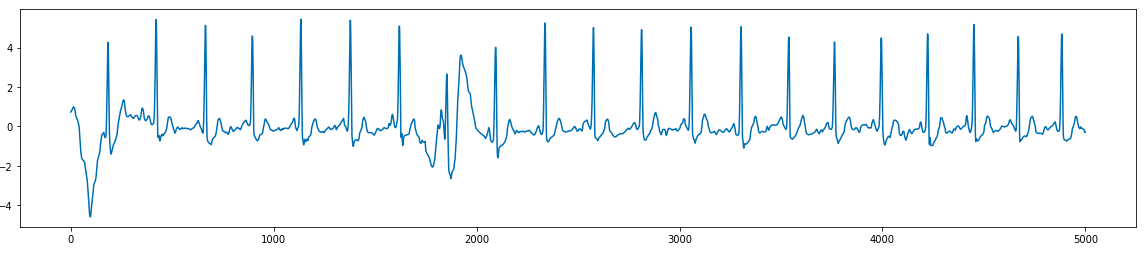
\includegraphics[width=15cm,height=4cm]{Normal.png}
            \caption{Ritmo Sinusal Normal}
            \label{fig:normal}
        \end{figure}
        
        
        \begin{figure}[H]
            \centering
            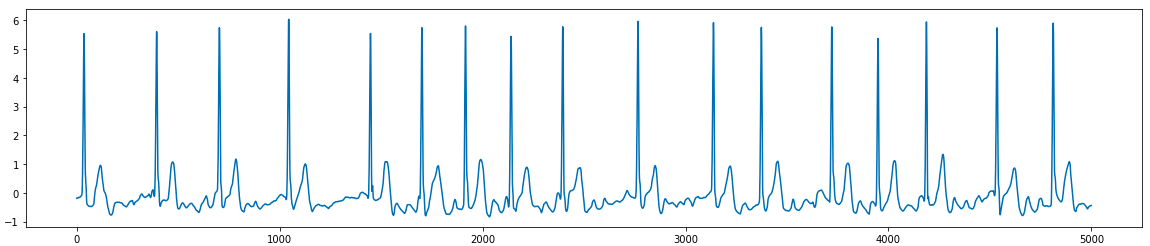
\includegraphics[width=15cm,height=4cm]{FA.png}
            \caption{Fibrilación Auricular}
            \label{fig:af}
        \end{figure}
        
        \begin{figure}[H]
            \centering
            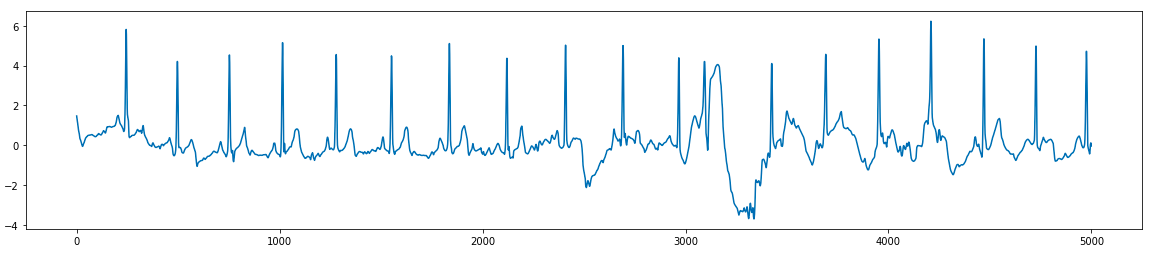
\includegraphics[width=15cm,height=4cm]{Other.png}
            \caption{Otro ritmo}
            \label{fig:other}
        \end{figure}
        
        \begin{figure}[H]
            \centering
            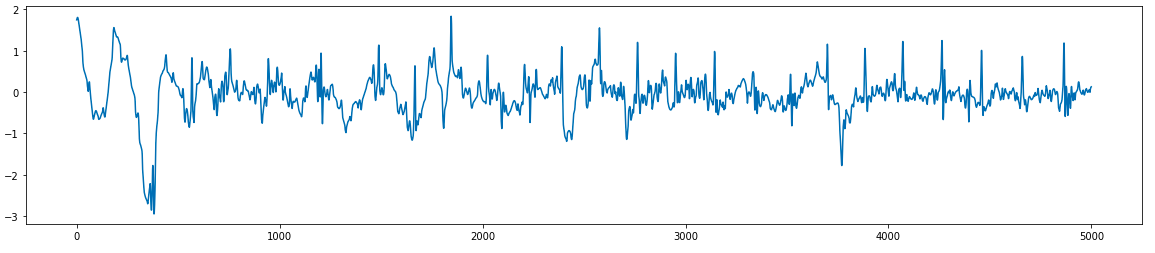
\includegraphics[width=15cm,height=4cm]{noise.png}
            \caption{Electrocardiograma Ruidoso}
            \label{fig:noise}
        \end{figure}
        

        En las figuras \ref{fig:normal},\ref{fig:af},\ref{fig:other} y \ref{fig:noise} mostramos un ejemplo de como sería cada señal. Visualmente puede distinguirse presencia de un ruido en la señal correspondiente a la figura \ref{fig:noise} y \ref{fig:other}, pero nada que ver con \ref{fig:noise} la cual tiene ruido en cantidades excesivas. \\
        
        
        \begin{table}[htbp]
        \caption{Datos del conjunto de entrenamiento}
        \begin{center}
        \begin{tabular}{|l|r|r|r|r|r|r|}
        \hline
        \textbf{Tipo} & \multicolumn{1}{l|}{\textbf{Cantidad}} & \multicolumn{1}{l|}{\textbf{Media}} & \multicolumn{1}{l|}{\textbf{SD}} & \multicolumn{1}{l|}{\textbf{Max}} & \multicolumn{1}{l|}{\textbf{Mediana}} & \multicolumn{1}{l|}{\textbf{Min}} \\ \hline
        \textbf{Normal} & 5154 & 31,9 & 10 & 61 & 30 & 9 \\ \hline
        \textbf{AF} & 771 & 31,6 & 12,5 & 60 & 30 & 10 \\ \hline
        \textbf{Otro Ritmo} & 2557 & 34,1 & 11,8 & 60,9 & 30 & 9,1 \\ \hline
        \textbf{Ruido} & 46 & 27,1 & 9 & 60 & 30 & 10,2 \\ \hline
        \textbf{Total} & 8528 & 32,5 & 10,9 & 61 & 30 & 9 \\ \hline
        \end{tabular}
        \end{center}
        \label{table:BD}
        \end{table}
        
        De la tabla \ref{table:BD} podemos observar el notorio desbalanceo de clases en el conjunto de datos. La clase mayoritaria correspondiente a los ritmos normales presentan casi el $60\%$ de los datos y la minoritaria, un poco más del $3\%$. Esto viene a indicar que el proceso de aprendizaje va a ser una tarea complicada, pues los modelos se van a especializar en clasificar la clase mayoritaria dejando de lado la minoritaria. \\
        
        Para tratar este desbalanceo se pueden emplear infinidad de técnicas, aunque en el contexto de la competición no son todas válidas. Por ejemplo, se podría pensar en eliminar la clase minoritaria por tener una representación ínfima del conjunto, sin embargo, las reglas establecen que eso no debe hacerse, pues a fin de cuentas estaremos sesgando los resultados y bajo el supuesto de que el modelo se implemente en la práctica, resultará en algo muy poco fiable y propenso a fallos. Por otra parte existen técnicas específicas para tratar el desbalanceo de ECG. Algunos investigadores como Sanabila et al. \cite{sanabila2016generative} utilizaron el método de sobremuestreo generado (GenOMe) para resolver el problema de las arritmias desequilibradas, que generaba nuevos puntos de datos con distribuciones específicas (beta, gamma y gaussiana) como restricciones. Y otros como Rajesh y Dhuli \cite{rajesh2018classification} emplearon tres técnicas de preprocesamiento a nivel de datos en un conjunto de características extraídas para equilibrar la distribución de los latidos del ECG. Estas técnicas fueron el sobremuestreo y submuestreo aleatorio (ROU), la técnica de sobremuestreo minoritario sintético con submuestreo aleatorio (SMOTE + RU) y el equilibrio basado en la distribución DBB. Sin embargo, nosotros no emplearemos técnicas tan sofisticadas para tratar ese problema. Las técnicas empleadas entran en la parte del preprocesado de datos que se comentará en el capítulo siguiente. \\
        
    

\section{Estado del Arte}

El electrocardiograma (ECG) es la herramienta de diagnóstico más común con un bajo coste utilizada para detectar las señales eléctricas del corazón. Las señales cardíacas anormales se conocen como arritmia y puede ser peligrosa o, en la mayoría de los casos, puede causar incluso la muerte. La arritmia puede ser de distintos tipos, y puede ser detectada por una prueba de ECG. El cribado automatizado de la clasificación de la arritmia mediante los latidos del ECG se desarrolla desde hace años. Los sistemas automatizados que pueden adaptarse como herramienta para la clasificación de arritmias desempeñan un papel vital no solo para los pacientes, sino también para los médicos. Las técnicas de clasificación de arritmias automatizadas basadas en el aprendizaje profundo se han desarrollado con resultados de alta precisión, pero aún no han sido adoptadas por los profesionales de la salud como un enfoque generalizado porque en los estudios recientes los autores utilizaron datos de series temporales, que no son adaptables en diferentes entornos de aplicación.  \\
    
    
    Según los datos facilitados por la \href{http://www.who.int/mediacentre/factsheets/fs317/en/.}{Organización Mundial de la Salud (OMS)} en 2020 murieron entorno a 25 millones de personas debido a este tipo de patologías. La prueba del electrocardiograma (ECG) se utiliza como herramienta de diagnóstico en los centros sanitarios pero son los profesionales sanitarios los que diagnostican manualmente el estado del corazón del paciente interpretando la imagen del ECG. Gracias al avance de la tecnología, se han desarrollado varias herramientas de diagnóstico automático para la clasificación y detección de arritmias con el fin de asistir a los médicos.\\
    
    De este modo, se empezó a investigar de forma crítica los latidos del corazón y herramientas de detección y clasificación. Desde su comienzo hasta hoy, podemos distinguir dos tipos de metodologías empleadas. Por un lado tenemos a la más tradicional. Esta vertiente se caracteriza por la necesidad de que el investigador tenga un conocimiento a priori sobre el tema, pues es él mismo quien decide de manera manual qué características extraer de las señales y cómo hacerlo. Poco a poco fue entrando en juego técnicas de aprendizaje profundo las cuales son capaces de extraer características por cuenta propia sin necesidad de conocimiento a priori por parte del investigador. Destacamos el trabajo de Khan et al. \cite{khan2021cardiac} que proporciona una introducción muy completa de los estudios relacionados en el dominio del problema y propone una técnica basada en redes neuronales profundas, para la clasificación de tres tipos de latidos de arritmia. \\
    
    Las últimas tendencias que se están usando son las arquitecturas de aprendizaje profundo, tras el estudio de numerosos artículos publicados sobre clasificación de arritmias (\cite{ohshuli,GaoJunLi,chenchen, zhang2020ecg,lynn2019deep,yao2020multi,gao2021end,tan2018application,sajjad2020novel,zheng2020automatic,wang2019photovoltaic,kim2019predicting,kim2020ensemble,geng2020epileptic,fu2019hybrid,huang2020classification,lih2020comprehensive,wei2019early,kong2019convolution,yildirim2019new,cai2020accurate,hou2019lstm}) destaca que los métodos más comúnmente usados son las redes neuronales recurrentes (RNN), LSTM, Autoencoder, CNN,  DNN y redes de creencias profundas. De hecho, en la imagen \ref{fig:trend state of art} podemos apreciar la tendencia actual en el uso de técnicas empleadas para este problema. Observamos que por antonomasia la más empleada es la CNN, pues la que mejor se encarga de extraer las características. Le sigue las redes neuronales profundas junto con las redes neuronales recurrentes y las LSTM. El autoencoder es otra técnica muy usada la cual realiza una reducción de la dimensionalidad, y trata de generar una clase similar a su entrada original. En numerosos estudios de investigación se aplicaron variaciones de la arquitectura de una red neuronal profunda con LSTM y autoencoder. En particular en el estudio \cite{hou2019lstm}, el autor propuso una arquitectura de LSTM con autoencoder combinada con una máquina de soporte vectorial (SVM) para la clasificación de arritmias en ECG. La red basada en LSTM-AE se dedicaba a aprender las características de las señales del ECG mediante un modelo codificador que extrae información de alto nivel de las señales a través de la red LSTM y un modelo decodificador que reconstruye las señales a partir de las características de alto nivel extraídas. La SVM se usaba para clasificar las señales a partir de las características aprendidas. Los resultados del estudio demostraron que la técnica propuesta aprendía mejores características que el método tradicional y sin ningún conocimiento previo, presentando así un buen potencial. Otros estudios como \cite{yildirim2019new} combinaban CNN, LSTM y autoencoder produciendo de igual manera, resultados bastante satisfactorios.\\
    
    La CNN es considera una herramienta de vanguardia para la clasificación de arritmias, y se ha estudiado con diversas variaciones, como la unidimensional, la bidimensional o la combinación de ambas \cite{xiao2020heart,noman2019short}. Según \cite{xiao2020heart}, una nueva técnica de clasificación de arritmias consta de tres fases: preprocesamiento, arquitectura CNN unidimensional, y votación por mayoría para predecir el resultado final. Por otra parte, en \cite{noman2019short} se propuso un marco basado en una CNN unidimensional para el aprendizaje directo de características a partir de los latidos de arritmia sin procesar y una CNN bidimensional, que toma mapas de características de tiempo-frecuencia bidimensionales. \\ 
    
    A día de hoy, se ha desarrollado un sistema automatizado que predice resultados de alta precisión para la detección de arritmias, en embargo aún no puede ser adoptado por los profesionales del sector de la salud. Las principales preocupaciones que afectan al éxito de los sistemas de detección de arritmias desarrollados son (i) la selección manual de características, (ii) las técnicas utilizadas para la extracción de características, (iii) el algoritmo utilizado para la clasificación, y (iv) el uso de datos desequilibrados para la clasificación siendo este último el más importante. \\ 
    
    
    Comentar que todos los estudios consultados han usado bases de datos públicas y totalmente disponibles para la comunidad investigadora. El principal inconveniente que presentan es la escasa cantidad de instancias que presentan algunas. En la imagen \ref{fig:db ecg} observamos las distintas bases de datos empleadas. Comentar que la mayoría no son específicas a su contexto clínico. Falta la descripción de la población de pacientes en la que se obtuvieron estos ECG, algo de vital importancia para poder interpretar la metodología y la utilidad clínica en su contexto. 
    
    \begin{figure}[htpb]
        \centering
        \includegraphics[scale=0.4]{img/state of art image.png}
        \caption{Tendencia actual de las técnicas usadas para clasificación de arritmias.Imagen obtenida de \cite{khan2021arrhythmia}}
        \label{fig:trend state of art}
    \end{figure}
    
    \begin{figure}
        \centering
        \includegraphics[width=\textwidth,height=\textheight,keepaspectratio]{img/database table.png}
        \caption{Base de datos de ECG dedicadas a clasificación de arritmias. Imagen obtenida de \cite{khan2021arrhythmia}}
        \label{fig:db ecg}
    \end{figure}
    
    
    

    
\endinput
% !TeX root = ../libro.tex
% !TeX encoding = utf8



\setchapterpreamble[c][0.75\linewidth]{%
	\sffamily
  
    Este capítulo pondrá en conocimiento al lector sobre los aspectos más técnicos que se han llevado a cabo para la elaboración del problema. Primeramente se comenzará hablando del software implementado que se ha empleado y de las cuestiones más importantes del mismo sin entrar mucho en detalle. Posteriormente se comentará el preprocesado realizado en los datos. Tras lo cual, se discutirá sobre la métrica empleada para la evaluación y posterior comparación entre los modelos. Finalmente se esclarecerá el método de selección de los modelos adelantando que será una variación del tradicional método de validación cruzada.
  

	\par\bigskip
}

\chapter{Contexto Experimental}\label{ch:contexto_experimental}


%%%%%%%%%%%%%%%%%%%%%%%%%%%%%%%%%%%%%%%%%%%%%%%%%%%%%%%%%%%%%%%%%%%%%%%%%%%%%%%%%%%%%%%%
%%%%%%%%%%%%%%%%%%%%%%%%%%%%%%%%%%%%%%%%%%%%%%%%%%%%%%%%%%%%%%%%%%%%%%%%%%%%%%%%%%%%%%%%
%%%%%%%%%%%%%%%%%%%%%%%%%%%%%%%%%%%%%%%%%%%%%%%%%%%%%%%%%%%%%%%%%%%%%%%%%%%%%%%%%%%%%%%%

\section{Software}

    El software ha sido implementado en Python, un lenguaje orientado a objetivos muy reconocido por la gran cantidad de herramientas que ofrece. Como librerías se han usado tensorflow junto con keras para la implementación de los modelos además de otras librerías auxiliares: numpy, pandas, seaborn, matplotlib, csv, math, time, sys, os, Sciky-Learn...\\
    
    Para el desarrollo del proyecto ha sido necesario el desarrollo de un conjunto de tres clases cuyos diagramas los podemos encontrar en las figuras \ref{fig:DC1} y \ref{fig:DC2}. Explicamos a continuación la labor que realiza cada una de ellas. La razón de los atributos de instancia así como la funcionalidad de los métodos están comentados en el código por lo que no entraremos en detalle en esa parte, solo mencionaremos las partes más importantes.\\
    
    \begin{itemize}
        \item DataReader: Esta clase está dedicada a la lectura de datos de fichero. El método principal es \textit{\_load\_data} el cual se encarga de leer los datos y no hay que llamarlo, el constructor lo llama directamente una vez se instancia la clase. Únicamente nos tenemos que preocupar de llamar al método \textit{get\_samples\_labels} que es el que nos devuelve los datos leído de fichero, tanto las señales como sus correspondientes etiquetas. 
        \item DataGenerator: Esta clase está dedicada a realizar el aumento de datos. Una vez instanciada podemos generar nuevas señales a partir de las iniciales llamando a los métodos \textit{amp\_signal}, \textit{vertical\_shift}, \textit{horizontal\_shift} y \textit{peaks\_noise}.
        \item CrossValidation: Esta es la clase más importante y se dedica a entrenar el modelo mediante validación cruzada y a sacar los resultados por fichero. Le pasamos al constructor los datos, el modelo junto con una gran cantidad de parámetros. El método principal se llama \textit{cross\_validate} y es al que tenemos que llamar una vez hayamos instanciado la clase. Este método se encarga por dentro de compilar el modelo, entrenarlo mediante validación cruzada y de imprimir los resultados por fichero. Es cierto que se podía haber atomizado más y separarlos en otros métodos. Sin embargo no se ha seguido esta vía ya que se quería hacer un código a muy alto nivel en el que solo se tenga que instanciar el objeto y realizar una única llamada a un método para obtenerlo todo. Esto miso es aplicable a la clase \textit{DataReader}
    \end{itemize}
    
    
    Un fichero llamado \textit{utils.py} ha sido también necesario para definir algunas funciones que nos resultarán de utilidad. El fichero \textit{models.py} contiene los modelos que se han empleado. El resto de ficheros con extensión \textit{.py} son aquellos dedicados a ser ejecutados. Los ficheros con extensión \textit{.sh} son scripts de bash que se han desarrollado con el objetivo de generar una capa de abstracción, de este modo, solo basta ejecutar el scrips y por dentro éste se encarga de iniciar el entorno virtual, buscar un nodo GPU que no esté ocupado, algunas opciones de configuración y de ejecutar el fichero con extensión \textit{.py}. \\
    
    

        \begin{figure}[H]
             \centering
             \begin{subfigure}[b]{0.3\textwidth}
             \includegraphics[scale=0.5]{img/DiagramaClase_DataReader.png}
             \caption{Diagrama de clase de la clase DataReader}
             \label{fig:DC_DataReader}
             \end{subfigure}
             \hfill
             \begin{subfigure}[b]{0.3\textwidth}
             \includegraphics[scale=0.5]{img/DiagramaClase_DataGenerator.png}
             \caption{Diagrama de clase de la clase DataGenerator}
             \label{fig:DC_DataGenerator}
             \end{subfigure}
             \caption{Diagrama de clases de las clases desarrolladas en el proyecto}
             \label{fig:DC1}
         \end{figure}
         \newpage
         \begin{figure}[H]
             \centering
             \includegraphics[scale=0.6]{img/DiagramaClase_CrossValidation.png}
             \caption{Diagrama de clase de la clase CrossValidation}
             \label{fig:DC2}
         \end{figure}
         

%%%%%%%%%%%%%%%%%%%%%%%%%%%%%%%%%%%%%%%%%%%%%%%%%%%%%%%%%%%%%%%%%%%%%%%%%%%%%%%%%%%%%%%%
%%%%%%%%%%%%%%%%%%%%%%%%%%%%%%%%%%%%%%%%%%%%%%%%%%%%%%%%%%%%%%%%%%%%%%%%%%%%%%%%%%%%%%%%
%%%%%%%%%%%%%%%%%%%%%%%%%%%%%%%%%%%%%%%%%%%%%%%%%%%%%%%%%%%%%%%%%%%%%%%%%%%%%%%%%%%%%%%%

\section{Preprocesado}

    La parte del preprocesado de los datos es una de las partes más importantes en ciencia de datos, ya que datos de calidad, aportan resultados de calidad, por lo que no debemos descuidar esta fase. De hecho, la misma plataforma de \textit{physionet} recomiendo tratar los datos antes de aplicar los modelos.\\
    
    \begin{figure}[H]
             \centering
             \begin{subfigure}[b]{0.4\textwidth}
             \includegraphics[scale=0.5]{img/trans_ampl.png}
             \caption{Amplificación}
             \label{fig:data_aug_ampl}
             \end{subfigure}
             \hfill
             \begin{subfigure}[b]{0.4\textwidth}
             \includegraphics[scale=0.5]{img/trans_ruido.png}
             \caption{Picos de Ruido}
             \label{fig:data_aug_ruido}
             \end{subfigure}
             
             \hfill
             
             \begin{subfigure}[b]{0.4\textwidth}
             \includegraphics[scale=0.5]{img/trans_horizontal.png}
             \caption{Desplazamiento horizontal}
             \label{fig:data_aug_horizontal}
             \end{subfigure}
             \hfill
             \begin{subfigure}[b]{0.4\textwidth}
             \includegraphics[scale=0.5]{img/trans_vertical.png}
             \caption{Desplazamiento vertical}
             \label{fig:data_aug_vertical}
             \end{subfigure}
             
             \caption{Transformaciones llevadas a cabo para el aumento de datos. La transformacione se han llevado a cabo sobre la gráfica de una distribución normal de media cero y varianza uno.}
             \label{fig:data_aug}
         \end{figure}
         
    Primeramente se leen los datos en crudo, ocurre que las señales no presentan todas el mismo tamaño, lo que supone un problema para los modelos. Debido a esto se ha de unificar el tamaño de las señales. Para ello se pensaron en muchas alternativas, la primera fue añadir zero-padding a las señales de menor longitud. Este enfoque en la práctica se tradujo en resultados pésimos, ya que las señales más pequeñas, que eran la mayoría, tras añadir el padding, se transformaban en una señal casi constantemente igual a cero. Tras esta perspectiva se decidió fijar un tamaño de ventana y leer de cada señal un subconjunto de la misma de tamaño igual al fijado por la ventana, de este modo evitamos el padding y las señales no son constantemente cero. Había que tener en cuenta que el tamaño de la ventana tenía que ser el suficientemente grande para contener así varios pulsos. Un tamaño de ventana entre 1000 y 5000 es el ideal. \\
    
    
    Tras la lectura de las señales, las normalizamos a media cero y desviación típica uno restando por la media y dividiendo por la desviación típica y teniendo en cuenta los datos que van a parar al conjunto de entrenamiento y al de test para de este modo no cometer \textit{data snooping}. \\ 
    
    Para tratar este desbalanceo se pueden emplear infinidad de técnicas, aunque en el contexto de la competición no son todas válidas. Por ejemplo, se podría pensar en eliminar la clase minoritaria por tener una representación ínfima del conjunto, sin embargo, las reglas establecen que eso no debe hacerse, pues a fin de cuentas, estaremos contaminando los resultados y bajo el supuesto de que el modelo se implemente en la práctica, resultará en algo muy poco fiable y propenso a fallos. De este modo, optamos por la técnica de aumento de datos, para ello nos dedicamos a hacer transformaciones con las señales originales para tener una mayor y variedad. Las distintas transformaciones realizadas las podemos encontrar en la figura \ref{fig:data_aug} donde podemos observar que se hemos realizado desplazamientos horizontales \ref{fig:data_aug_horizontal} y verticales \ref{fig:data_aug_vertical}, amplificaciones de la señal \ref{fig:data_aug_ampl} y picos de ruido \ref{fig:data_aug_ruido}. En la práctica los resultados empeoraban con estas transformaciones y por este motivo se decidió no incluirlas. \\
    
    




%%%%%%%%%%%%%%%%%%%%%%%%%%%%%%%%%%%%%%%%%%%%%%%%%%%%%%%%%%%%%%%%%%%%%%%%%%%%%%%%%%%%%%%%
%%%%%%%%%%%%%%%%%%%%%%%%%%%%%%%%%%%%%%%%%%%%%%%%%%%%%%%%%%%%%%%%%%%%%%%%%%%%%%%%%%%%%%%%
%%%%%%%%%%%%%%%%%%%%%%%%%%%%%%%%%%%%%%%%%%%%%%%%%%%%%%%%%%%%%%%%%%%%%%%%%%%%%%%%%%%%%%%%

\section{Métrica}
    
    Existen una amplia gama de métricas que evalúan el rendimiento de los modelos, en nuestro caso hemos usado la métrica conocida como $F1$. Presentamos primero la matriz de confusión, en la que la posición $(i,j)$ representa el número de ejemplos de la clase $i$ que han sido predichos como elementos de la clase $j$. En la imagen $\ref{fig:metrica}$ también se incluye una columna y una fila adicional que representan la suma de todos los elementos totales de cada clase y la suma del número de prediciones realizadas para esa misma clase. La diagonal de la matriz de confusión aparecen los elementos correctamente clasificados y en la práctica es lo que nos gustaría maximizar. El resto de entradas a excepción de la diagonal y las celdas marginales añadidas, representan instancias mal clasificadas.
    
    \begin{figure}[H]
        \centering
        \includegraphics[scale=0.5]{img/metrica.png}
        \caption{Regla para contar el número de variables. En verde se presentan los elementos correctamente clasificados, en azul los incorrectamente clasificados y en naranja y rosa la suma de las columnas y filas respectivamente. \href{https://physionet.org/files/challenge-2017/1.0.0/table3.png}{Fuente}}
        \label{fig:metrica}
    \end{figure}
    
    Para cada una de las clases calculamos su respectiva métrica $F_1$-score de la siguiente manera:
    
    \begin{itemize}
        \item Ritmo normal:
        \begin{equation}
            F_{1n} = \frac{2 Nn}{\sum_{N} + \sum_{n}}
        \end{equation}
        \item Ritmo AF:
        \begin{equation}
            F_{1a} = \frac{2 Aa}{\sum_{N} + \sum_{n}}
        \end{equation}
        \item Otro ritmo:
        \begin{equation}
            F_{1o} = \frac{2 Oo}{\sum_{O} + \sum_{o}}
        \end{equation}
        \item Ruido:
        \begin{equation}
            F_{1p} = \frac{2 Pp}{\sum_{P} + \sum_{p}}
        \end{equation}
    \end{itemize}
    
    \noindent Finalmente, la métrica $F1$ es la media aritmética de estas cuatro,
    \begin{equation}
        F1 = \frac{F_{1n} + F_{1a} + F_{1o} + F_{1p}}{4}
    \end{equation}
    
    El motivo principal existente en cuanto a la elección de esta métrica no es más que subsanar el desbalanceo entre clases otorgando la misma importancia a cada una de ellas. Esto no ocurre en el caso de otras métricas como por ejemplo la \textit{precisión} o \textit{accuracy} la cual expresa el cociente del número de instancias bien clasificadas dividido por el total de instancias. De este modo, en el problema que nos atañe, ocurriría que si un modelo responde correctamente a todos los ejemplos de la clase mayoritaria (Ritmo Normal) y equivocadamente al resto tendría una precisión inferior a $0.6$, lo que nos puede llevar a pensar que el modelo, aunque se equivoque en el $40\%$ de las veces, tiene capacidad de predicción (¡Algo falso!). Del mismo modo y aplicando la métrica $F1$ se obtendría un valor inferior a $0.2$, por lo que de este modo, esta métrica fuerza a construir un modelo en el que la predicción correcta de cada clase influya por igual independientemente del desbalanceo. \\
    
%%%%%%%%%%%%%%%%%%%%%%%%%%%%%%%%%%%%%%%%%%%%%%%%%%%%%%%%%%%%%%%%%%%%%%%%%%%%%%%%%%%%%%%%
%%%%%%%%%%%%%%%%%%%%%%%%%%%%%%%%%%%%%%%%%%%%%%%%%%%%%%%%%%%%%%%%%%%%%%%%%%%%%%%%%%%%%%%%
%%%%%%%%%%%%%%%%%%%%%%%%%%%%%%%%%%%%%%%%%%%%%%%%%%%%%%%%%%%%%%%%%%%%%%%%%%%%%%%%%%%%%%%%

\section{Método de selección de los modelos}

    

    Esta competición cuenta con un conjunto de datos de test a los cuales no hemos tenido acceso por lo que solo hemos empleado los datos de entrenamiento. La selección de los modelos se ha hecho por medio de una variación de la validación cruzada con 5 \textit{folds} la cual se está empezando a emplear mucho en la literatura y consiste en entrenar, validar y aplicar el test en cada fold. \\
    
    Al emplear 5 \textit{folds} realizamos 5 entrenamientos con los datos, en cada entrenamiento dividimos los datos en un conjunto disjunto de entrenamiento, validación y test mediante un muestreo aleatorio estratificado, $S_{train}^i, S_{val}^i$ y $S_{test}^i$ de tal manera que ${S_{train}^i \cap S_{test}^i \cap S_{val}^i = \emptyset}$ y ${S_{train}^i \cup S_{test}^i \cup S_{val}^i = S}$ para $i=\{1,2,3,4,5\}$ . Además, se ha de cumplir que $\bigcap_j S_{test}^j = \emptyset$. Con el muestreo aleatorio estratificado conseguimos que haya la misma proporción de instancias de cada clase en las particiones que el conjunto original. Tras este particionado, se entrena con $S_{train}$, validamos con $S_{val}$ y evaluamos con $S_{test}$.  \\
    
    El motivo de lo anterior es sencillo, obviamente necesitamos el conjunto $S_{train}$ para poder entrenar los datos, el conjunto $S_{val}$ lo usamos para tomar decisiones sobre el entrenamiento, como por ejemplo, la parada del \textit{Early Stopping}, observar la curva de aprendizaje o valorar si se produce o no sobreentrenamiento. Finalmente, $S_{test}$ lo usamos para ver como generaliza y para sacar conclusiones con respecto a otros modelos haciendo así a esta variación de validación cruzada mucho más robusta que la original porque no solo obtenemos la media aritmética de los resultados en cuanto al entrenamiento, sino que también en cuanto a generalización, es decir, en el conjunto de test. \\
    
    Tras la obtención de los resultados en todos los modelos empleados, se elige como modelo ganador aquel con mejores puntuaciones en la métrica $F1$ obtenida con los datos proporcionados por el conjunto de test. \\



\endinput
% !TeX root = ../libro.tex
% !TeX encoding = utf8



\setchapterpreamble[c][0.75\linewidth]{%
	\sffamily
    
    En esta sección se expondrá el desarrollo de los cuatro mejores modelos de la competición llevada a cabo en el año 2017 por la plataforma PhysioNet en la que se usó la misma base de datos la cual se está empleando. También se detallaran tres modelos que se avalan en la literatura por presentar buenos resultados en los problemas para los que fueron planteados. Por último y más importante, se expondrán tres modelos desarrollados propiamente para este problema.
  

	\par\bigskip
}

\chapter{Desarrollo de los modelos}\label{ch:desarrollo}

\section{Modelos Ganadores de la Competición}
        

        Todos los modelos ganadores usan un paradigma común que funciona en dos partes. En la primera se extraen un conjunto de características sobre el problema y en la segunda parte, se aplica clasificación sobre dicho conjunto, lo único que varía son los métodos de extracción y clasificación. Esta forma tiene un ligero problema y es que para la extracción de características los autores requieren de cierto conocimiento previo sobre el campo en cuestión, en este caso ha sido posible, pero de manera general no siempre va a ocurrir. Otro inconveniente es la poca transportabilidad de estos modelos frente a otros problemas. Esto es debido a que los modelos son particularmente diseñados para un problema muy concreto, luego si los intentamos extrapolar a otros ámbitos, posiblemente fallen. 
        
    \subsection{Clasificador binario en cascada}
       
             El artículo de este modelo se puede encontrar en \cite{datta2017identifying}. Los autores consideraron una serie de 209 características que podían ser útiles a la hora de clasificar. Para ello la agruparon en un total de siete conjuntos: Características enfocadas en ECGs con ruido, en particulares de ciertas patologías, en estadísticas, en frecuencias, sobre el ritmo cardiaco, sobre la morfología del ECG y por último en características utilizadas en trabajos anteriores. \\
             
             Tras extraer las características se aplica un clasificador binario en cascada en dos fases. En la primera, el clasificador es entrenado con el objetivo de distinguir entre ECGs normales o con otras patologías y ECGs con fibrilación auricular o ruidosos, es decir, junta la clases N y O por un lado y por otro las clases FA y R para clasificarlas. En la segunda fase se consideran dos nuevos clasificadores. Uno de ellos clasifica las clases N y O que previamente se habían juntado y el otro las clases FA y R. \\ 
             
    \subsection{Encase}
        
            Este modelo es un clasificador diseñado por ensemble, esto es, un clasificador construido a partir de un conjunto de clasificadores resumiendo la salida para obtener una única predicción. Este método lo que primero hace es descomponer el ECG en un conjunto de datos más reducido. Tras hacer esta separación se calcula la onda más informativa del electrocardiograma, conocida como \textit{centerwave} y después se aplican varios extractores de características para terminar aplicando el ensemble de clasificadores. \\
            
            En el funcionamiento que hemos explicado hemos obviado una gran cantidad de detalles, este modelo es el más complejo de todos y se puede consultar en \cite{hong2017encase}
            
          
        
    \subsection{Marco de Interpretación Abductivo}
        
            Este método parte de la creación de un marco de razonamiento completo que trabaja con señales temporales médicas. Destacamos que este método fue diseñado por investigadores españoles de la universidad de Santiago de Compostela, \cite{teijeiro2017arrhythmia}. Primeramente, se extrae la información sobre la morfología del ECG por medio del razonador abducctivo y se construyen 79 característias globales del electrocardiograma. Después se aplica un algoritmo de \textit{gradient boosing} combinado con una red neuronal recurrente y un voto por ponderación para realizar la clasificación. \\
        
    \subsection{Clasificador basado en Random Forest}
            
            Este algoritmo también aplica la extracción de características de manera manual y después se aplica un clasificador simple para ordenarlas por orden de importancia a la hora de clasificar señales. Según se explica en \cite{zabihi2017detection} se generaron un total de 491 características para después aplicar un \textit{random forest} y seleccionar la 150 más informativas. Tras ello, se diseña un clasificador para realizar las predicciones sobre el conjunto reducido. \\
    
    
\newpage 
\section{Modelos en la Literatura}

    Vamos a exponer un conjunto de arquitecturas encontradas en la literatura que presentan buenos resultados según los autores. Comentamos previamente que las arquitecturas son fijas en el sentido de que no se ha realizado ninguna prueba para escoger los hiperparámetros de los modelos ya que de hacerse así se estaría contaminando la arquitectura tomada de la literatura. \\
    
    Existen otros parámetros como el algoritmo de optimización, el tamaño del batch, tamaño de ventana etcétera que si convendrían escogerlos de manera experimental. Se realizó pues un proceso experimental probando distintos hiperparámetros, sin embargo, la mayoría presentaban los mismos resultados, puesto que como más adelante se comentará, estos modelos dan lugar a un gran sobreajuste y la elección de los hiperparámetros no influye apenas. Por este motivo, se omitirá la parte experimental. 
    
    
    \begin{table}[H]
        \caption{Hiperparámetros usados en los modelos. Para OhShuLih y GaoJunLi el tamaño de ventana es igual a 3000 mientras que para ChenChen es la propia arquitectura la que exige un tamaño de ventana algo mayor, por este motivo se ha tomado 5000. El optimizador usado ha sido \textit{Adam} con el learning rate que presenta por defecto. Adam es un optimizador muy recomendable en la literatura y de ahí su elección. El tamaño del batch no puede ser muy grande ya que origina un fallo en la memoria de los servidores GPU, pero tampoco puede ser demasiado pequeño por temas de eficiencia, de este modo, se ha considerado como óptimo el seleccionado. El número de épocas empleadas han sido 300 para que la red se entrene lo suficiente, aunque a veces no se lleguen a completarlas todas gracias a la técnicas de Early Stopping con valor de la paciencia 50. Por otra parte, se ha reducido el tamaño de la serie porque si se deja toda la longitud, los resultados empeoran. En cuanto a la generación de datos, los resultados empeoran si se activa y por este motivo se ha desactivado. }
        \begin{center}
        \begin{tabular}{|l|l|}
        \hline
        \multicolumn{1}{|c|}{\textbf{Parámetros}} & \multicolumn{1}{l|}{Valores} \\ \hline
        \textbf{Batch size} & 128 \\ \hline
        \textbf{Epochs} & 300 \\ \hline
        \textbf{Patiente} & 50 \\ \hline
        \textbf{n\_split} & 5 \\ \hline
        \textbf{reduce} & True \\ \hline
        \textbf{generator} & False \\ \hline
        \textbf{windows\_size} & 3000-5000 \\ \hline
        \textbf{lr} & 0,001 \\ \hline
        \textbf{opt} & Adam \\ \hline
        \end{tabular}
        \end{center}
        \label{fig:hiper_lit}
    \end{table}
    
    \subsection{OhShuLi}
    
        Presentamos un modelo presente en la literatura \cite{ohshuli}, al cual nos referiremos con el nombre del autor, OhShuLih. En el artículo se comenta los buenos resultados que ofrece esta arquitectura, la cual consta de 6 capas convolucionales en las que se incluyen capas de max pooling. Estas capas se encargan de extraer características espaciales de las señales y la última capa de LSTM se encarga de capturar la dependencia en la dinámica temporal de la serie. Finalmente se incluyen tres capas totalmente conectadas. En la imagen \ref{fig:ohshuli_1} podemos ver la arquitectura de esta red en el artículo en donde fue propuesta. \\
        
        \begin{figure}[htpb]
            \centering
            \includegraphics[height=20cm,width=17cm,keepaspectratio]{img/ohshuli1.png}
            \caption{Una ilustración de la arquitectura OhShuLi}
            \label{fig:ohshuli_1}
        \end{figure}
        
        \begin{figure}[htpb]
            \centering
            \includegraphics[width=\textwidth,height=\textheight,keepaspectratio]{img/ohshuli_plot.png}
            \caption{Esquema de la arquitectura OhShuLi. Parámetros entrenables $3254$. Esta arquitetura consta de 3 capas convolucionales de 3, 6 y 6 filtros con un tamaño de kernel de 20,10 y 5 respectivamente. La celda LSTM consta de 20 unidades y las capas capas totalmente conectadas constan de 20,10 y 4 neuronas respectivamente.}
            \label{fig:ohshuli_2}
        \end{figure}
        
        
        
        
    \subsection{ChenChen}
    
        Esta arquitectura la podemos encontrar en \cite{chenchen}. En este artículo se comenta brevemente por encima las ventajas y desventajas de los métodos existentes en cuanto a diagnósticos clínicos, tras lo cual se propone esta arquitectura (Fig \ref{fig:chenchen1},\ref{fig:chenchen2}) con el objetivo de analizar y reconocer seis clases de segmentos de ECG, incluyendo N, AFIB, B, P, AFL y ABR. El artículo justifica el empleo de capas CNN+LSTM explicando que las capas convolucionales se encaran de la extracción automática de características, y el empleo de LSTM se usa en el intervalo entre dos picos R adyacentes para mejorar el rendimiento de identificación. La combinación de CNN más LSTM contribuyen a la extración de información espacial y temporal de las señales y a la mejora de la capacidad de abstracción del modelo. Este artículo empleó como bases de datos: \textit{MIT-BITH}, \textit{AFDB} y \textit{NSRDB}. \\
    
            \begin{figure}[htpb]
                \centering
                \includegraphics[width=\textwidth,height=\textheight,keepaspectratio]{img/chenchen2.png}
                \caption{Esquema de la arquitectura ChenChen. Parámetros entrenables: $91751$}
                \label{fig:chenchen2}
            \end{figure}
            
            \begin{figure}[htpb]
                \centering
                \includegraphics[height=17cm,width=15cm,keepaspectratio]{img/chenchen1.png}
                \caption{Una ilustración de la arquitectura ChenChen. Se han aplicado 6 capas de convolución con 251,150,100,81,61 y 14 filtros y con un tamaño del kernel de 5,5,10,20,20,10 respectivamente. Las capas LSTM tienen 32 y 64 unidades cada una respectivamente.}
                \label{fig:chenchen1}
            \end{figure}
        
    
    
        
    \subsection{GaoJunLi}
    
    Este modelo fue propuesto en \cite{GaoJunLi} y es específico para conjunto de datos con desbalanceo de clase, de hecho el nombre del artículo es \textit{An Effective LSTM Recurrent Network to Detect Arrhythmia on Imbalanced ECG Dataset}. El artículo argumenta que el desequilibrio del conjunto de datos del ECG es un reto adicional para clasificar con precisión los latidos del ECG. Hay dos problemas en el proceso de entrenamiento: (1) la baja eficiencia del entrenamiento, porque los latidos normales del ECG que ocupan una gran proporción del conjunto de datos son propensos a los efectos negativos, y (2) la degeneración del modelo cuando un latido normal del ECG sobrecarga el entrenamiento. Tras lo cual comenta que algunos investigadores han intentado abordar el desequilibrio en los datos de los latidos del ECG a la hora de diagnosticar la arritmia siendo este artículo uno de esos intentos. \\
    
    
    Dado que los datos de los latidos del ECG existen en una categoría muy desequilibrada, se propone un modelo eficaz de red de recurrencia de memoria a corto plazo (LSTM) con pérdida focal (FL). Para ello, la red LSTM puede desentrañar las características de sincronización en las señales complejas de ECG, mientras que la FL se utiliza para resolver el desequilibrio de categorías mediante la reducción de la ponderación de los ejemplos de ECG normales fácilmente identificados. Las ventajas de la red propuesta se han verificado en la base de datos de arritmias MIT-BIH. Los resultados experimentales muestran que la red LSTM con FL logró una solución fiable al problema de los conjuntos de datos desequilibrados en la clasificación de latidos de ECG y no fue sensible a la calidad de las señales de ECG. El método propuesto puede utilizarse en escenarios de telemedicina para ayudar a los cardiólogos a diagnosticar con mayor precisión y objetividad las señales de ECG. En la imagen \ref{fig:gaojunlin} podemos ver la arquitectura de esta red.  \\
    
    
    
        \begin{figure}[htpb]
                \centering
                \includegraphics[width=\textwidth,height=\textheight,keepaspectratio]{img/GaoJunLin.png}
                \caption{Esquema de la arquitectura GaoJunLin. Total de parámetros entrenables: $19108$ }
                \label{fig:gaojunlin}
        \end{figure}
            
\newpage
\section{Modelos propios}
    
        Tres propuestas distintas de modelos propios se han desarrollado, el primer modelo basado puramente en convoluciones unidimensionales lo llamaremos CNN, el segundo modelos además de convoluciones unidimensionales tiene unidades LSTM y por ello lo denotaremos con el nombre LSTM y finalmente el tercer y último tipo de modelo lo llamaremos GRU por estar formado por unidades GRU además de convoluciones unidimensionales. \\
        
        La elección de los parámetros tales como el número de filtros de las capas convolucionales, el tamaño del kernel, así como el número de unidades GRU y LSTM y algunos otros parámetos como el nivel de \textit{drop out} o el tipo de padding fueron escogidos en base a un proceso experimental expuesto en la siguiente sección. Otros hiperparámetros, como los de la tabla \ref{fig:hiper_lit} los hemos fijado de antemano.\\
        
        La arquitectura de los modelos (escogidas según el proceso de experimentación que se expondrá en la sección siguiente) las podemos apreciar en las tablas \ref{table:arquitectura modelo cnn}, \ref{table:arquitectura modelo lstm} y \ref{table:arquitectura modelo gru}. En las cuales podemos ver el tipo de capa, el tamaño de la salida y el número de unidades que componen las capas de convolución (unidades entendidas como filtros) y las capas densas (unidades entendidas como neuronas). \\
        
    \subsection{CNN}
        Los hiperparámetros tuneados en este modelo han sido el porcentage de \textit{drop out}, el número de filtros, el tamaño del kernel y el tipo de padding. El \textit{drop out} es un aspecto clave que contribuye a la disminución de sobreajuste. El número de filtros convolucionales y el tamaño del kernel son los dos aspectos más importantes de las redes convolucionales, por lo que un estudio previo sobre los parámetros oportunos es de obligado cumplimiento. El tipo de \textit{padding} es algo que afeta en menor medida, aún así se ha decidido estudiar qué influencia tiene. En la tabla \ref{table:arquitectura modelo cnn} podemos ver la arquitectura. \\
        
        \begin{table}[htpb]
            \caption{Arquitectura Modelo CNN}
            \begin{center}
            %\resizebox{\columnwidth}{!}{%
            \begin{tabular}{|l|l|r|}
            \hline
            \textbf{Layer} & \textbf{Output Shape} & \multicolumn{1}{l|}{\textbf{Units}} \\ \hline
            Conv1D + ReLu + MaxPooling & (None,3000,256) & 128 \\ \hline
            MaxPooling + Drop Out & (None,1500,256) & 0 \\ \hline
            Conv1D + ReLu & (None,1500,256) & 128 \\ \hline
            MaxPooling + Drop Out & (None,750,256) & 0 \\ \hline
            Conv1D + ReLu & (None,750,128) & 64 \\ \hline
            MaxPooling + Drop Out & (None,375,128) & 0 \\ \hline
            Conv1D + ReLu & (None,375,85) & 42 \\ \hline
            MaxPooling + Drop Out & (None,187,85) & 0 \\ \hline
            Conv1D + ReLu & (None,187,64) & 32 \\ \hline
            MaxPooling + Drop Out & (None,93,64) & 0 \\ \hline
            Conv1D + ReLu & (None,93,51) & 25 \\ \hline
            MaxPooling + Drop Out & (None,46,51) & 0 \\ \hline
            Conv1D + ReLu & (None,46,42) & 21 \\ \hline
            MaxPooling + Drop Out & (None,23,256) & 0 \\ \hline
            Global Average Pooling & (None,42) & 0 \\ \hline
            Dense + Relu + Drop Out & (None,128) & 128 \\ \hline
            Dense + Relu + Drop Out & (None,64) & 64 \\ \hline
            Dense + Relu + Drop Out & None,32) & 32 \\ \hline
            Dense + Softmax & (None,4) & 0 \\ \hline
            \textbf{Total Parámetros} & 1288656 & \\ \hline
            \end{tabular}
            %}
            \end{center}
            \label{table:arquitectura modelo cnn}
            \end{table}
    
    \subsection{LSTM}
        Los parámetros usados para este modelo han sido las unidades de LSTM, las neuronas de las últimas capas densas y el tipo de padding. El número de unidades en la capa LSTM es un aspecto fundamental y que no debe de ser pasado por alto. El número de unidades en las últimas capas densas también es importante por ese motivo también ha sido estudiado. Notamos que el número de hiperparámetros aquí es mucho menor que el anterior, esto se debe en parte a que este tipo de modelos gastan gran cantidad de tiempo en ejecución dificultando la realización de un estudio más detallado. El valor de \textit{drop out} se ha fijado a $0,4$. En la tabla \ref{table:arquitectura modelo lstm} podemos ver la arquitectura. \\
        
    
        \begin{table}[htpb]
            \caption{Arquitectura Modelo LSTM}
            \begin{center}
            %\resizebox{\columnwidth}{!}{%
            \begin{tabular}{|l|l|r|}
            \hline
            \textbf{Layer} & \textbf{Output Shape} & \multicolumn{1}{l|}{\textbf{Units}} \\ \hline
            Input & (None,3000,1) & 0 \\ \hline
            Zero Padding & (None,3008,1) & 0 \\ \hline
            Conv1D & (None,3004,128) & 128 \\ \hline
            Max Pooling & (None,1502,128) & 0 \\ \hline
            Zero Padding & (None,1510,128) & 0 \\ \hline
            Conv1D & (None,1506,64) & 64 \\ \hline
            Max Pooling & (None,753,64) & 0 \\ \hline
            Zero Padding & (None,761,64) & 0 \\ \hline
            Conv1D & (None,757,32) & 32 \\ \hline
            Max Pooling & (None,378,32) & 0 \\ \hline
            Zero Padding & (None,386,32) & 0 \\ \hline
            Conv1D & (None,382,8) & 8 \\ \hline
            Max Pooling & (None,191,8) & 0 \\ \hline
            LSTM + Drop Out & (None,16) & 16 \\ \hline
            Dense + ReLu + Drop Out & (None,32) & 32 \\ \hline
            Dense + Softmax & (None,4) & 4 \\ \hline
            \textbf{Total Parámetros} & 55396 & \\ \hline
            \end{tabular}
            %}
            \end{center}
            \label{table:arquitectura modelo lstm}
            \end{table}
            
    \subsection{GRU}
    
        Los parámetros usados para este modelo han sido el número de unidades GRU y el número de neuronas en las capas densas. Estos dos hiperparámetros son los más importantes del modelo y los de obligatorio estudio. El resto de hiperparámetros se han fijado a un valor y no se han tenido en cuenta para el estudio por los motivos expuestos en el modelo anterior. El valor de \textit{drop out} se ha fijado a $0,4$. En la tabla \ref{table:arquitectura modelo gru} podemos ver la arquitectura. \\
        
    
        
            \begin{table}[htpb]
            \caption{Arquitectura Modelo GRU}
            \begin{center}
            %\resizebox{\columnwidth}{!}{%
            \begin{tabular}{|l|l|r|}
            \hline
            \textbf{Layer} & \textbf{Output Shape} & \multicolumn{1}{l|}{\textbf{Units}} \\ \hline
            Input & (None,3000,1) & 0 \\ \hline
            Zero Padding & (None,3008,1) & 0 \\ \hline
            Conv1D & (None,3004,128) & 128 \\ \hline
            MaxPooling & (None,1502,128) & 0 \\ \hline
            Zero Padding & (None,1510,128) & 0 \\ \hline
            Conv1D & (None,1506,64) & 64 \\ \hline
            Max Pooling & (None,753,64) & 0 \\ \hline
            Zero Padding & (None,761,64) & 0 \\ \hline
            Conv1D & (None,757,32) & 32 \\ \hline
            Max Pooling & (None,378,32) & 0 \\ \hline
            Zero Padding & (None,386,32) & 0 \\ \hline
            Conv1D & (None,382,8) & 8 \\ \hline
            Max Pooling & (None,191,8) & 0 \\ \hline
            GRU + Drop Out & (None,25) & 25 \\ \hline
            Dense + ReLu + Drop Out & (None,32) & 32 \\ \hline
            Dense + Softmax & (None,4) & 4 \\ \hline
            \textbf{Total Parámetros} & 56709 & \\ \hline
            \end{tabular}
            %}
            \end{center}
            \label{table:arquitectura modelo gru}
            \end{table}


%        \newpage
%        \begin{figure}[H]
%             \centering
%             \begin{subfigure}[b]{0.3\textwidth}
%             \includegraphics[height=\textheight,keepaspectratio]{img/arq_mod_1_1.png}
%             \end{subfigure}
%             \hfill
%             \begin{subfigure}[b]{0.3\textwidth}
%             \includegraphics[height=\textheight,keepaspectratio]{img/arq_modelo_1_2.png}
%             \end{subfigure}
%             \caption{Esquema de la arquitectura CNN.}
%             \label{fig:arquitectura modelo cnn}
%         \end{figure}
%
%       
%        \begin{figure}[H]
%                \centering
%                \includegraphics[width=\textwidth,height=\textheight,keepaspectratio]{img/modelo2.png}
%                \caption{Esquema de la arquitectura LSTM.}
%               \label{fig:arquitectura modelo lstm}
%        \end{figure} 
%        
%        \begin{figure}[H]
%                \centering
%                \includegraphics[width=\textwidth,height=\textheight,keepaspectratio]{img/modelo2.png}
%                \caption{Esquema de la arquitectura GRU.}
%                \label{fig:arquitectura modelo gru}
%        \end{figure} 
        
        
       
    
    

    
\endinput
% !TeX root = ../libro.tex
% !TeX encoding = utf8



\setchapterpreamble[c][0.75\linewidth]{%
	\sffamily
  
    En este capítulo se mostraran los resultados obtenidos de dos de los cuatro mejores modelos de la competición, los resultados obtenido de los modelos propuestos por la literatura y los resultados de los modelos propios. Además, para la elección de los hiperparámetros óptimos en las propuestas propias de modelo, se ha realizado un proceso experimental el cual también se expondrá. Tras ello, se procederá a realizar un análisis detenido en detalle sobre los resultados obtenidos que culminará con una comparación entre todos los modelos.
  

	\par\bigskip
}

\chapter{Resultados y Análisis}\label{ch:analisis}


%%%%%%%%%%%%%%%%%%%%%%%%%%%%%%%%%%%%%%%%%%%%%%%%%%%%%%%%%%%%%%%%%%%%%%%%%%%%%%%%%%%%%%%%
%%%%%%%%%%%%%%%%%%%%%%%%%%%%%%%%%%%%%%%%%%%%%%%%%%%%%%%%%%%%%%%%%%%%%%%%%%%%%%%%%%%%%%%%
%%%%%%%%%%%%%%%%%%%%%%%%%%%%%%%%%%%%%%%%%%%%%%%%%%%%%%%%%%%%%%%%%%%%%%%%%%%%%%%%%%%%%%


\section{Resultados}

    En esta sección presentamos los resultados de los modelos anteriormente comentados a excepción del marco de interpretación abductivo y el modelo ENCASE, los cuales no han podido ser reproducidos.
    
    \subsection{Modelos ganadores de la competición}
    

        \begin{table}[H]
        \caption{Resultados de dos de los cuatro modelos ganadores. Clasificador basado en Randon Forest y Clasificador Binario en Cascada}
        \begin{center}
        \begin{tabular}{|c|r|r|}
        \hline
        & \multicolumn{1}{l|}{\textbf{Clasif. Random Forest}} & \multicolumn{1}{l|}{\textbf{Clasif. B. Cascd.}} \\ \hline
        \textbf{Fn} & 0,916 & 0,892 \\ \hline
        \textbf{Fa} & 0,827 & 0,768 \\ \hline
        \textbf{Fo} & 0,786 & 0,722 \\ \hline
        \textbf{Fr} & 0,617 & 0,584 \\ \hline
        \textbf{F1} & 0,787 & 0,741 \\ \hline
        \end{tabular}
        \end{center}
        \label{table:resultados_modelosganadores}
        \end{table}

        \begin{table}[H]
        \caption{Matriz de Confusión del clasificador basado en Random Forest}
        \begin{center}
        \begin{tabular}{|c|r|r|r|r|}
        \hline
        \multicolumn{1}{|l|}{} & \multicolumn{1}{l|}{\textbf{Normal}} & \multicolumn{1}{l|}{\textbf{FA}} & \multicolumn{1}{l|}{\textbf{Otro}} & \multicolumn{1}{l|}{\textbf{Ruido}} \\ \hline
        \textbf{Normal} & 953 & 2 & 57 & 3 \\ \hline
        \textbf{FA} & 5 & 116 & 29 & 2 \\ \hline
        \textbf{Otro} & 92 & 10 & 375 & 6 \\ \hline
        \textbf{Ruido} & 15 & 1 & 10 & 29 \\ \hline
        \end{tabular}
        \end{center}
        \label{table:RF_CM}
        \end{table}


    

        \begin{table}[H]
        \caption{Matriz de confusión del clasificador binario en cascada}
        \begin{center}
        \begin{tabular}{|c|r|r|r|r|}
        \hline
        \multicolumn{1}{|l|}{} & \multicolumn{1}{l|}{\textbf{Normal}} & \multicolumn{1}{l|}{\textbf{FA}} & \multicolumn{1}{l|}{\textbf{Otro}} & \multicolumn{1}{l|}{\textbf{Ruido}} \\ \hline
        \textbf{Normal} & 962 & 7 & 53 & 6 \\ \hline
        \textbf{FA} & 6 & 114 & 28 & 4 \\ \hline
        \textbf{Otro} & 118 & 21 & 333 & 10 \\ \hline
        \textbf{Ruido} & 15 & 4 & 7 & 31 \\ \hline
        \end{tabular}
        \end{center}
        \label{table:CBC_CM}
        \end{table}


    
    
    
    \subsection{Modelos propuestos por la literatura}
    
    
          
        \begin{table}[H]
        \caption{Matriz de Confusión GaoJunLi}
        \begin{center}
        \begin{tabular}{|l|r|r|r|r|}
        \hline
         & \multicolumn{1}{l|}{\textbf{Normal}} & \multicolumn{1}{l|}{\textbf{FA}} & \multicolumn{1}{l|}{\textbf{Otro}} & \multicolumn{1}{l|}{\textbf{Ruido}} \\ \hline
        \textbf{Normal} & 1011 & 0 & 0 & 0 \\ \hline
        \textbf{FA} & 147 & 0 & 0 & 0 \\ \hline
        \textbf{Otro} & 491 & 0 & 0 & 0 \\ \hline
        \textbf{Ruido} & 57 & 0 & 0 & 0 \\ \hline
        \end{tabular}
        \end{center}
        \label{table:GaoJunLin_CM}
        \end{table}
        
        
        \begin{table}[H]
        \caption{Matriz de Confusión del modelo ChenChen}
        \begin{center}
        \begin{tabular}{|l|r|r|r|r|}
        \hline
         & \multicolumn{1}{l|}{\textbf{Normal}} & \multicolumn{1}{l|}{\textbf{FA}} & \multicolumn{1}{l|}{\textbf{Otro}} & \multicolumn{1}{l|}{\textbf{Ruido}} \\ \hline
        \textbf{Normal} & 873 & 2 & 92 & 0 \\ \hline
        \textbf{FA} & 122 & 1 & 11 & 0 \\ \hline
        \textbf{Otro} & 431 & 2 & 43 & 0 \\ \hline
        \textbf{Ruido} & 38 & 0 & 1 & 0 \\ \hline
        \end{tabular}
        \end{center}
        \label{table:ChenChen_CM}
        \end{table}
        
        \begin{table}[H]
        \caption{Matriz de Confusión del modelo OhShuLi}
        \begin{center}
        \begin{tabular}{|l|r|r|r|r|}
        \hline
         & \multicolumn{1}{l|}{\textbf{Normal}} & \multicolumn{1}{l|}{\textbf{FA}} & \multicolumn{1}{l|}{\textbf{Other}} & \multicolumn{1}{l|}{\textbf{Ruido}} \\ \hline
        \textbf{Normal} & 980 & 0 & 29 & 0 \\ \hline
        {\textbf{FA}} & 141 & 0 & 6 & 0 \\ \hline
        \textbf{Other} & 470 & 0 & 20 & 0 \\ \hline
        \textbf{Ruido} & 52 & 0 & 5 & 0 \\ \hline
        \end{tabular}
        \end{center}
        \label{cm_ohsuli}
        \end{table}

        
        \begin{table}[H]
        \caption{Resultados de los modelos OhShuLi, ChenChen y GaoJunLi}
        \begin{center}
        \begin{tabular}{|l|r|r|r|}
        \hline
         & \multicolumn{1}{l|}{\textbf{GaoJunLi}} & \multicolumn{1}{l|}{\textbf{ChenChen}} & \multicolumn{1}{l|}{\textbf{OhShuLi}} \\ \hline
        \textbf{Test loss} & 0,986 & 1,302 & 0,833 \\ \hline
        \textbf{Test accuracy} & 0,591 & 0,631 & 0,652 \\ \hline
        \textbf{Test sco} & 0,201 & 0,279 & 0,341 \\ \hline
        \textbf{Fn} & 0,743 & 0,776 & 0,793 \\ \hline
        \textbf{Fa} & 0 & 0,149 & 0,193 \\ \hline
        \textbf{Fo} & 0,034 & 0,192 & 0,31 \\ \hline
        \textbf{Fr} & 0,068 & 0,088 & 0,249 \\ \hline
        \textbf{F1} & 0,211 & 0,301 & 0,386 \\ \hline
        \end{tabular}
        \end{center}
        \label{table:results_litera}
        \end{table}


        \begin{figure}[H]
            \centering
            \includegraphics[width=\textwidth,height=\textheight,keepaspectratio]{img/ChenChen_epoch_sco.png}
            \caption{Modelo ChenChen - El eje X representa el avance de las épocas y el eje Y la métrica $F_1$. La curva naranja representa el entrenamiento y la azul la validación.}
            \label{fig:chenchen_tensorboard}
        \end{figure}
        
        \begin{figure}[H]
            \centering
            \includegraphics[width=\textwidth,height=\textheight,keepaspectratio]{img/ohshuli_epoch_sco.png}
            \caption{Modelo OhShuLi - El eje X representa el avance de las épocas y el eje Y la métrica $F_1$.La curva naranja representa el entrenamiento y la azul la validación.}
            \label{fig:ohshuli_tensorboard}
        \end{figure}
        
        \begin{figure}[H]
            \centering
            \includegraphics[width=\textwidth,height=\textheight,keepaspectratio]{img/GaoJunLi_epochsco.png}
            \caption{Modelo GaoJunLi - El eje X representa el avance de las épocas y el eje Y la métrica $F_1$.La curva naranja representa el entrenamiento y la azul la validación.}
            \label{fig:gaojunli_tensorboard}
        \end{figure}
    
    
    
    \subsection{Modelos propios}
    
    
    \begin{table}[H]
    \caption{Resultados de la fase de experimentación del modelo LSTM. Los resultados están ordenados de manera decreciente según el valor de la métrica $F_1$.}
    \begin{center}
    \begin{tabular}{|r|r|r|l|r|r|r|r|r|}
    \hline
    \multicolumn{1}{|l|}{} & \multicolumn{1}{l|}{\textbf{lstm\_units}} & \multicolumn{1}{l|}{\textbf{dense\_units}} & \textbf{padding} & \multicolumn{1}{l|}{\textbf{Fn}} & \multicolumn{1}{l|}{\textbf{Fa}} & \multicolumn{1}{l|}{\textbf{Fo}} & \multicolumn{1}{l|}{\textbf{Fr}} & \multicolumn{1}{l|}{\textbf{F1}} \\ \hline
    1 & 16 & 32 & same & 0,8485 & 0,3117 & 0,5246 & 0,3611 & 0,5115 \\ \hline
    2 & 16 & 32 & valid & 0,8394 & 0,3457 & 0,5273 & 0,2632 & 0,4939 \\ \hline
    3 & 16 & 8 & valid & 0,8409 & 0,2221 & 0,5166 & 0,1543 & 0,4335 \\ \hline
    4 & 8 & 8 & same & 0,8042 & 0,5443 & 0,3057 & 0,0000 & 0,4136 \\ \hline
    5 & 16 & 8 & same & 0,8457 & 0,1243 & 0,5321 & 0,1307 & 0,4082 \\ \hline
    6 & 8 & 32 & same & 0,7914 & 0,3447 & 0,3572 & 0,1055 & 0,3997 \\ \hline
    7 & 8 & 32 & valid & 0,7945 & 0,2970 & 0,2949 & 0,1675 & 0,3885 \\ \hline
    8 & 4 & 8 & valid & 0,7864 & 0,3630 & 0,1944 & 0,0000 & 0,3360 \\ \hline
    9 & 8 & 8 & valid & 0,7889 & 0,2269 & 0,2939 & 0,0000 & 0,3274 \\ \hline
    10 & 4 & 8 & same & 0,7885 & 0,2576 & 0,2581 & 0,0000 & 0,3261 \\ \hline
    11 & 4 & 32 & valid & 0,7593 & 0,0425 & 0,1605 & 0,0000 & 0,2406 \\ \hline
    12 & 4 & 32 & same & 0,7412 & 0,0000 & 0,0859 & 0,0000 & 0,2068 \\ \hline
    \end{tabular}
    \end{center}
    \label{table:model2_result}
    \end{table}
    
    \begin{table}[htbp]
        \caption{Resultados de la fase de experimentación del primer modelo GRU. Los resultados están ordenados de manera decreciente según el valor de la métrica $F_1$.}
        \begin{center}
        \begin{tabular}{|r|l|r|r|r|r|r|r|r|}
        \hline
        \multicolumn{1}{|l|}{} & \textbf{drop} & \multicolumn{1}{l|}{\textbf{gru\_units}} & \multicolumn{1}{l|}{\textbf{dense\_units}} & \multicolumn{1}{l|}{\textbf{Fn}} & \multicolumn{1}{l|}{\textbf{Fa}} & \multicolumn{1}{l|}{\textbf{Fo}} & \multicolumn{1}{l|}{\textbf{Fr}} & \multicolumn{1}{l|}{\textbf{F1}} \\ \hline
        1 & 0.4 & 25 & 32 & 0,8715 & 0,6682 & 0,5921 & 0,4415 & 0,6433 \\ \hline
        2 & 0.4 & 25 & 64 & 0,8699 & 0,6681 & 0,5871 & 0,4308 & 0,6390 \\ \hline
        3 & 0.4 & 16 & 32 & 0,8642 & 0,5345 & 0,5428 & 0,4751 & 0,6042 \\ \hline
        4 & 0.4 & 16 & 32 & 0,8591 & 0,5949 & 0,5284 & 0,3728 & 0,5888 \\ \hline
        5 & 0.4 & 16 & 64 & 0,8566 & 0,5208 & 0,5411 & 0,3722 & 0,5727 \\ \hline
        6 & 0.4 & 4 & 8 & 0,7586 & 0,2969 & 0,2170 & 0,0795 & 0,3380 \\ \hline
        7 & 0.4 & 16 & 8 & 0,8333 & 0,0000 & 0,4466 & 0,0069 & 0,3217 \\ \hline
        8 & 0.4 & 8 & 32 & 0,8027 & 0,1059 & 0,3110 & 0,0389 & 0,3146 \\ \hline
        9 & 0.4 & 8 & 8 & 0,7670 & 0,0000 & 0,1165 & 0,0000 & 0,2209 \\ \hline
        10 & 0.4 & 4 & 32 & 0,7438 & 0,0000 & 0,0000 & 0,0000 & 0,1860 \\ \hline
        \end{tabular}
        \end{center}
        \label{table:model3_result}
        \end{table}
    

        \begin{table}[H]
        \caption{Resultados de la fase de experimentación del modelo CNN. Los resultados están ordenados de manera decreciente según el valor de la métrica $F_1$.}
        \begin{center}
        \resizebox{\columnwidth}{!}{%
        \begin{tabular}{|r|l|r|r|l|r|r|r|r|r|}
        \hline
        \multicolumn{1}{|l|}{\textbf{Nº}} & \textbf{drop} & \multicolumn{1}{l|}{\textbf{filters}} & \multicolumn{1}{l|}{\textbf{kernel}} & \textbf{padding} & \multicolumn{1}{l|}{\textbf{Fn}} & \multicolumn{1}{l|}{\textbf{Fa}} & \multicolumn{1}{l|}{\textbf{Fo}} & \multicolumn{1}{l|}{\textbf{Fr}} & \multicolumn{1}{l|}{\textbf{F1}} \\ \hline
        1 & 0.4 & 256 & 9 & same & 0,8785 & 0,7360 & 0,6340 & 0,5194 & 0,6920 \\ \hline
        2 & 0.4 & 256 & 7 & same & 0,8809 & 0,7393 & 0,6457 & 0,4893 & 0,6888 \\ \hline
        3 & 0.4 & 128 & 3 & same & 0,8802 & 0,7384 & 0,6378 & 0,4834 & 0,6850 \\ \hline
        4 & 0.4 & 128 & 5 & same & 0,8830 & 0,7144 & 0,6359 & 0,5062 & 0,6849 \\ \hline
        5 & 0.2 & 128 & 3 & same & 0,8800 & 0,7309 & 0,6469 & 0,4676 & 0,6814 \\ \hline
        6 & 0.2 & 64 & 5 & same & 0,8790 & 0,7221 & 0,6233 & 0,4831 & 0,6769 \\ \hline
        7 & 0.4 & 128 & 3 & same & 0,8808 & 0,7137 & 0,6325 & 0,4757 & 0,6757 \\ \hline
        8 & 0.4 & 128 & 7 & same & 0,8819 & 0,7345 & 0,6481 & 0,4294 & 0,6735 \\ \hline
        9 & 0.4 & 256 & 3 & same & 0,8808 & 0,7137 & 0,6508 & 0,4443 & 0,6724 \\ \hline
        10 & 0.4 & 512 & 3 & same & 0,8768 & 0,7237 & 0,6310 & 0,4561 & 0,6719 \\ \hline
        11 & 0.2 & 128 & 5 & valid & 0,8749 & 0,7080 & 0,6217 & 0,4740 & 0,6696 \\ \hline
        12 & 0.4 & 128 & 5 & valid & 0,8743 & 0,7248 & 0,6062 & 0,4519 & 0,6643 \\ \hline
        13 & 0.2 & 128 & 3 & valid & 0,8741 & 0,7019 & 0,6129 & 0,4652 & 0,6635 \\ \hline
        14 & 0.4 & 128 & 3 & valid & 0,8725 & 0,6875 & 0,6102 & 0,4479 & 0,6545 \\ \hline
        15 & 0.2 & 64 & 3 & same & 0,8711 & 0,6887 & 0,5844 & 0,4525 & 0,6492 \\ \hline
        16 & 0.2 & 64 & 3 & valid & 0,8683 & 0,6675 & 0,5830 & 0,4663 & 0,6463 \\ \hline
        17 & 0.2 & 64 & 5 & valid & 0,8667 & 0,6701 & 0,5730 & 0,4306 & 0,6351 \\ \hline
        18 & 0.4 & 64 & 5 & valid & 0,8678 & 0,6663 & 0,5655 & 0,4223 & 0,6305 \\ \hline
        19 & 0.4 & 64 & 3 & valid & 0,8655 & 0,6680 & 0,5518 & 0,4187 & 0,6260 \\ \hline
        20 & 0.2 & 32 & 5 & same & 0,8642 & 0,6292 & 0,5408 & 0,4167 & 0,6127 \\ \hline
        21 & 0.4 & 128 & 9 & same & 0,8530 & 0,5855 & 0,5167 & 0,4097 & 0,5912 \\ \hline
        22 & 0.4 & 128 & 5 & same & 0,8537 & 0,5833 & 0,5160 & 0,4072 & 0,5900 \\ \hline
        23 & 0.2 & 128 & 5 & same & 0,8532 & 0,5829 & 0,5202 & 0,3860 & 0,5856 \\ \hline
        24 & 0.4 & 256 & 5 & same & 0,8525 & 0,5921 & 0,5193 & 0,3671 & 0,5827 \\ \hline
        25 & 0.4 & 64 & 5 & same & 0,8492 & 0,5731 & 0,4794 & 0,3866 & 0,5721 \\ \hline
        26 & 0.4 & 64 & 3 & same & 0,8453 & 0,4730 & 0,4599 & 0,4012 & 0,5449 \\ \hline
        27 & 0.4 & 32 & 3 & same & 0,8552 & 0,3575 & 0,4957 & 0,3792 & 0,5219 \\ \hline
        28 & 0.2 & 32 & 3 & same & 0,8492 & 0,3099 & 0,5126 & 0,3674 & 0,5098 \\ \hline
        29 & 0.2 & 32 & 3 & valid & 0,8516 & 0,2824 & 0,5466 & 0,3524 & 0,5082 \\ \hline
        30 & 0.2 & 32 & 5 & valid & 0,8533 & 0,2384 & 0,5265 & 0,3087 & 0,4817 \\ \hline
        31 & 0.4 & 512 & 9 & same & 0,8244 & 0,4191 & 0,3801 & 0,2798 & 0,4759 \\ \hline
        32 & 0.4 & 32 & 5 & valid & 0,8512 & 0,0936 & 0,5242 & 0,3929 & 0,4655 \\ \hline
        33 & 0.4 & 32 & 5 & same & 0,8500 & 0,1079 & 0,5182 & 0,3492 & 0,4563 \\ \hline
        34 & 0.4 & 32 & 3 & valid & 0,8469 & 0,0216 & 0,5272 & 0,3184 & 0,4285 \\ \hline
        35 & 0.4 & 512 & 5 & same & 0,7719 & 0,1527 & 0,1282 & 0,0917 & 0,2861 \\ \hline
        36 & 0.4 & 512 & 7 & same & 0,7709 & 0,1478 & 0,1316 & 0,0898 & 0,2850 \\ \hline
        \end{tabular}
        }
        \end{center}
        \label{table:model1_result}
        \end{table}


        
        
        \begin{table}[htbp]
        \caption{Matriz de confusión del modelo GRU}
        \begin{center}
        \begin{tabular}{|l|r|r|r|r|}
        \hline
        \textbf{} & \multicolumn{1}{l|}{\textbf{Normal}} & \multicolumn{1}{l|}{\textbf{FA}} & \multicolumn{1}{l|}{\textbf{Otras}} & \multicolumn{1}{l|}{\textbf{Ruido}} \\ \hline
        \textbf{Normal} & 934 & 6 & 69 & 0 \\ \hline
        \textbf{FA} & 114 & 6 & 27 & 0 \\ \hline
        \textbf{Otras} & 375 & 9 & 106 & 0 \\ \hline
        \textbf{Ruido} & 50 & 1 & 6 & 0 \\ \hline
        \end{tabular}
        \end{center}
        \label{table:CM gru}
        \end{table}

        
      \begin{table}[htbp]
        \caption{Matriz de confusión del modelo LSTM}
        \begin{center}
        \begin{tabular}{|l|r|r|r|r|}
        \hline
        \textbf{} & \multicolumn{1}{l|}{\textbf{Normal}} & \multicolumn{1}{l|}{\textbf{FA}} & \multicolumn{1}{l|}{\textbf{Otras}} & \multicolumn{1}{l|}{\textbf{Ruido}} \\ \hline
        \textbf{Normal} & 927 & 0 & 82 & 0 \\ \hline
        \textbf{FA} & 127 & 0 & 20 & 0 \\ \hline
        \textbf{Otras} & 422 & 0 & 68 & 0 \\ \hline
        \textbf{Ruido} & 51 & 0 & 6 & 0 \\ \hline
        \end{tabular}
        \end{center}
        \label{table:CM lstm}
        \end{table}
  
        \begin{table}[htbp]
        \caption{Matriz de confusión del modelo CNN}
        \begin{center}
        \begin{tabular}{|l|r|r|r|r|}
        \hline
         & \multicolumn{1}{l|}{\textbf{Normal}} & \multicolumn{1}{l|}{\textbf{FA}} & \multicolumn{1}{l|}{\textbf{Otras}} & \multicolumn{1}{l|}{\textbf{Ruido}} \\ \hline
        \textbf{Normal} & 941 & 6 & 62 & 0 \\ \hline
        \textbf{FA} & 117 & 10 & 20 & 0 \\ \hline
        \textbf{Otras} & 371 & 9 & 110 & 0 \\ \hline
        \textbf{Ruido} & 49 & 2 & 6 & 0 \\ \hline
        \end{tabular}
        \end{center}
        \label{table:CM cnn}
        \end{table}


        \begin{figure}[H]
            \centering
            \includegraphics[width=\textwidth,height=\textheight,keepaspectratio]{img/curva modelo 1_best.png}
            \caption{Curva aprendizaje modelo CNN - El eje X representa el avance de las épocas y el eje Y la métrica $F_1$.La curva naranja representa el entrenamiento y la azul la validación.}
            \label{fig:curva_model1}
        \end{figure}
        
        
        
        \begin{figure}[H]
            \centering
            \includegraphics[width=\textwidth,height=\textheight,keepaspectratio]{img/curva modelo2_best.png}
            \caption{Curva aprendizaje modelo LSTM - El eje X representa el avance de las épocas y el eje Y la métrica $F_1$.La curva naranja representa el entrenamiento y la azul la validación.}
            \label{fig:curva_model2}
        \end{figure}
        
        
        
        \begin{figure}[H]
            \centering
            \includegraphics[width=\textwidth,height=\textheight,keepaspectratio]{img/curva modelo3_best.png}
            \caption{Curva aprendizaje modelo GRU - El eje X representa el avance de las épocas y el eje Y la métrica $F_1$.La curva naranja representa el entrenamiento y la azul la validación.}
            \label{fig:curva_model3}
        \end{figure}


        \begin{table}[htbp]
        \caption{Resultados de los mejores modelos de cada tipo obtenidos en el proceso de experimentación.}
        \begin{center}
        \begin{tabular}{|l|r|r|r|}
        \hline
        \textbf{} & \multicolumn{1}{l|}{\textbf{LSTM}} & \multicolumn{1}{l|}{\textbf{GRU}} & \multicolumn{1}{l|}{\textbf{CNN}} \\ \hline
        \textbf{Fn} & 0,849 & 0,871 & 0,879 \\ \hline
        \textbf{Fa} & 0,312 & 0,668 & 0,736 \\ \hline
        \textbf{Fo} & 0,525 & 0,592 & 0,634 \\ \hline
        \textbf{Fr} & 0,361 & 0,442 & 0,519 \\ \hline
        \textbf{F1} & 0,511 & 0,643 & 0,692 \\ \hline
        \end{tabular}
        \end{center}
        \label{table:MejoresModelosPropios}
        \end{table}

    
    
    \begin{table}[H]
        \caption{Resultados del todo el conjunto de modelos estudiados. Los resultados están ordenados de manera decreciente según el valor de la métrica $F_1$.}
        \begin{center}
        \begin{tabular}{|l|r|r|r|r|r|}
        \hline
        \textbf{} & \multicolumn{1}{l|}{\textbf{Fn}} & \multicolumn{1}{l|}{\textbf{Fa}} & \multicolumn{1}{l|}{\textbf{Fo}} & \multicolumn{1}{l|}{\textbf{Fr}} & \multicolumn{1}{l|}{\textbf{F1}} \\ \hline
        \textbf{RF} & 0,916 & 0,827 & 0,786 & 0,617 & 0,787 \\ \hline
        \textbf{B. Cascada} & 0,892 & 0,768 & 0,722 & 0,584 & 0,741 \\ \hline
        \textbf{CNN} & 0,879 & 0,736 & 0,634 & 0,519 & 0,692 \\ \hline
        \textbf{GRU} & 0,871 & 0,668 & 0,592 & 0,442 & 0,643 \\ \hline
        \textbf{LSTM} & 0,849 & 0,312 & 0,525 & 0,361 & 0,511 \\ \hline
        \textbf{OhShuLi} & 0,793 & 0,193 & 0,31 & 0,249 & 0,386 \\ \hline
        \textbf{ChenChen} & 0,776 & 0,149 & 0,192 & 0,088 & 0,301 \\ \hline
        \textbf{GaoJunLi} & 0,743 & 0 & 0,034 & 0,068 & 0,211 \\ \hline
        \end{tabular}
        \end{center}
        \label{table:Comparativa Global}
    \end{table}
    
    
    \begin{figure}[H]
        \centering
        \includegraphics[scale=0.5]{img/grafica comparativa.png}
        \caption{Gráfica donde se puede apreciar de manera visual los resultados de la tabla \ref{table:Comparativa Global}}
        \label{fig:comparativa}
    \end{figure}

    

\section{Análisis}
    

    Entre los dos modelos ganadores de la competición que tenemos que según la tabla \ref{table:resultados_modelosganadores}, el que mejores resultados presenta es el clasificador basado en Random Forest. Comparando las matrices de confusión tenemos que la matriz del clasificador binario en cascada presenta más fallos al clasificar las clases \textit{FA}, \textit{Otro} y \textit{Ruido}. Esto lo podemos deducir gracias a la diagonal principal de la matriz. Por otro lado, el clasificador binario en cascada presenta una mayor tasa de aciertos en predecir los ritmos normales, sin embargo, el principal objetivo no es ese y además, el clasificador basado en Random Forest, aunque presente una menor cantidad de aciertos en clasificar ritmos normales que el otro, ocurre que el número de aciertos tampoco es que sea bajo, siendo la diferencia entre unos y otros bastante ajustada. De la matrices de confusión podemos observar un problema que atañe a ambos modelos y es la dificultad que existe a la hora de distinguir entre algunos electrocardiogramas sanos y otros que presentan un tipo de patología distinta a la fibrilación auricular. \\
    
    Los resultados de los modelos propuestos por la literatura son pésimos. Esto queda reflejado nada más ver las matrices de confusión de las tablas \ref{table:ChenChen_CM}, \ref{table:GaoJunLin_CM} y \ref{cm_ohsuli}. Observamos que el modelo GaoJunLi ha clasificado todas las instancias en una única clase, la mayoritaria. El modelo ChenChen, algo mejor que el anterior, no ha clasificado ninguna instancia como ruidosa y solo ha clasificado una instancia correcta de la clase \textit{FA}. El modelo OhShuLi solo ha sido capaz de clasificar en dos clases (Normal y ritmos con ruido ruido) dejando de lado al resto. La comparativa de los tres modelo la podemos encontrar en la tabla \ref{table:results_litera} donde vemos que el que mejores resultados presenta en términos de la métrica $F_1$ es el modelo OhShuLi. Obviamente, podemos ver que los modelos carecen de total interés. Pero indaguemos un poco más en el por qué de lo anterior.\\


    En \ref{fig:chenchen_tensorboard}, \ref{fig:gaojunli_tensorboard} y \ref{fig:ohshuli_tensorboard} presentamos del número de épocas en función del valor de la métrica. Estas curvas son bastante esclarecedoras por poner encima de la mesa el mal comportamiento de estos modelos. En la curva del modelo ChenChen, \ref{fig:chenchen_tensorboard}, observamos como la curva de entrenamiento, la naranja, crece en la primeras épocas y se mantiene oscilando pero con una tendencia constante, en cambio, la curva de validación en ningún momento aumenta. Esto nos hace ver que el modelo es incapaz de llevar a cabo un correcto aprendizaje en entrenamiento, pues los valores en el eje de ordenadas son pequeños y aún peor, que no ha sido capaz de generalizar al menos ni un poco. La gráfica del modelo OhShuLi, \ref{fig:ohshuli_tensorboard}, se ve un poco distinta a la anterior ya que la curva de validación no es constante. Podemos observar que durante las primeras épocas, el entrenamiento y la validación sí se mantuvieron constantes pero a partir de cierto momento comienzan a variar. Ambas curvas presentan una distancia muy pequeña algo que sí que es deseable, en cambio, se encuentran en un valor del eje de ordenadas insignificante, quizás más épocas hubieran sido necesarias, pero de ser así, el riesgo de sobreentrenamiento sería casi inminente. Finalmente, en la gráfica del modelo GaoJunLi, \ref{fig:gaojunli_tensorboard}, podemos apreciar una curva de aprendizaje algo más normal que las que vimos anteriormente. En las últimas épocas, la curva de entrenamiento crece abruptamente mientras la curva de validación mantiene su tendencia, lo que se puede interpretar como un posible sobreajuste. \\
    
    En resumen, los modelos propuestos por la literatura presentan malos resultados. Tenemos en cuenta que estos modelos fueron diseñados y refinados para datos pertenecientes a otra base de datos, y pese a que la finalidad haya sido la misma que la nuestra, no quiere decir que tengan que funcionar igual de bien con nuestros datos. Por otra parte comentar que el modelo ChenChen presenta bastante complejidad, es decir, demasiados grados de libertad por tener más capas convolucionales y más profundas además de dos capas LSTM con una gran cantidad de unidades. En cambio, modelo GaoJunLi puede parecer algo más simple, pues no presenta una fase de extracción de características usando CNN sino que directamente se aplican $64$ capas LSTM seguidas de capas densas, quizás este vacío haya ocasionado que únicamente clasifique según la clase mayoritaria. Aunque parezca que sea más simple, esto no quiera decir que actúe mejor, pues se piensan que $64$ capas LSTM es un número excesivo. Por otra parte, el modelo OhShuLih aunque presenta pocas capas convolucionales y de poca profundidad, el tamaño del kernel es bastante elevado. Esto hace que la extracción de características no sea fructífera, pues el tamaño de las series temporales no es demasiado grane. A todo esto se le suma la complejidad que presenta la base de datos, la cual no cuenta con una cantidad suficiente de datos y para más inri, tenemos un increíblemente fuerte desbalanceo entre clases. Todo lo anterior contribuye a que estos modelos proporcionen unos resultados bastante pobres. Esto nos sirve como ejemplo del teorema de No Free Lunch, ya que estas propuestas obtenidas de la literatura han dado buenos resultados para los problemas en los que fueron creados, pero malos resultados al realizar una tarea distinta. \\
    
    Ahora vamos a estudiar la propuestas de modelos propios. Empezamos por la selección de una hipótesis ganadora en cada modelo, para ello se han sometido cada uno a un proceso experimental en el que se ejecutan varias veces con distintos hiperparámetros. En la tabla \ref{table:model1_result} podemos observar todas las ejecuciones realizadas sobre el modelo CNN, obsevamos que el mejor valor de drop out entre los probados es de $0.4$, el número de filtros es de 235, el tamaño del kernel óptimo es de 9. En la tabla \ref{table:model2_result} podemos ver que los parámetros óptimos para el modelo LSTM son de 16 unidades en la capa de LSTM y 32 neuronas para las capas densas. Finalmente, en la tabla \ref{table:model3_result} vemos las distinta ejecuciones realizadas para el modelo GRU cuya mejor realización presenta un número de unidades GRU igual a 25 y 32 neuronas en las capas densas. \\
    
    En la tablas \ref{table:CM cnn}, \ref{table:CM lstm} y \ref{table:CM gru} presentamos las matrices de confusión de los modelos CNN, LSTM y GRU respectivamente. Observamos que ningún modelo ha sido capaz de predecir aquellos ritmos que presentan ruido y la mayoría han sido clasificados como ritmos sanos, lo cual es un desacierto pues lo que nos interesa no es saber los pacientes sanos, sino detectar los enfermos. También ocurre que todos los modelos presentan dificultad a la hora de clasificar instancias con fibrilación auricular, es decir, ninguno cumple con los objetivos que se pretendían alcanzar. Con esto vemos una clara limitación que los convierte también en modelos no deseables. \\
    
    
    En las imágenes \ref{fig:curva_model1}, \ref{fig:curva_model2} y \ref{fig:curva_model3} podemos observar las curvas de aprendizaje en las que el eje abscisas representa el número de épocas y el eje de ordenadas el valor de la métrica. En el modelo CNN podemos ver que durante las cien primeras épocas, tanto la curva de entrenamiento como la de validación van a la par. A partir de de ahí se distancian poco a poco. Mientras que la de entrenamiento adquiere una tendencia creciente, la de validación se mantiene constante. Con esto observamos que los resultados en validación no mejoran con el paso de las épocas pudiendo incurrir en sobreaprendizaje si se hubieran aplicado más épocas en el entrenamiento. La curva del modelo LSTM tiene un comportamiento muy llamativo durante las primeras épocas. Parece que no se produce un correcto entrenamiento durante las etapas más tempranas. En cambio, pasadas las primeras cien épocas, se observa que ambas curvan adquieren una tendencia creciente. Se puede también apreciar que pese a que ambas curvas sean crecientes, el incremente de la curva de entrenamiento es mayor que el de la curva de validación. Se puede llegar a pensar que más épocas hubieran hecho falta para estabilizar las curvas. Por último, las curvas del modelo GRU presentan una tendencia creciente y muy a la par. Ambas curvas no se separan demasiado la una de la otra, incluso en algunas partes podemos apreciar que la curva de validación supera a la de entrenamiento, suceso el cual no es muy normal que ocurra. \\
    
    
    En la tabla \ref{table:resultados_modelosganadores} podemos apreciar los resultados de los tres modelos que hemos propuesto. Observamos que el que mejor puntuación obtiene en todas las métricas es el modelo CNN, seguido del modelo GRU y por último, el modelo LSTM. Es interesante observar que pese a que el modelo LSTM y GRU tengan además de capas convolucionales, otras estructuras que en la teoría contribuyen al tratamiento de señales no hayan obtenido mejores resultados que el modelo puramente convolucional. Sin embargo, está bien comentar que el modelo CNN ha sido muy refinado en el proceso de experimentación por ser el más rápido en ser ejecutado, permitiendo así realizar un gran número de pruebas con diferentes hiperparámetros en pos de encontrar los óptimos. Esto mismo no ha sido posible con los otros dos modelos restantes debido a sus lentos tiempo de ejecución. Podemos llegar a pensar que tanto el modelo LSTM y GRU se hubieran podido pulir aún más para que presenten mejores resultados e incluso hubiesen podido superar al modelo CNN. \\ 
    
    
    Fijándonos en la tabla \ref{table:Comparativa Global} y a modo de conclusión, los modelos ganadores de la competición son los que mejores resultados presentan, pues fueron diseñados única y exclusivamente para esta base de datos por un equipo de profesionales cuyo objetivo era ganar la competición. El modelo RF es el mejor en todas las métricas así como el clasificador binario en cascada que es el segundo mejor en todas ellas. Los modelos empleados en la literatura, no son universales, es decir, no actúan igual de bien en todos los problemas y como consecuencia, tenemos lo sucedido. Los modelos propuestos en este trabajo no son tan sofisticados como los modelos ganadores, obteniendo peores resultados que estos, pero han sido más refinados para el problema que los encontrados en la literatura, logrando así resultados no tan malos. En la imagen \ref{fig:comparativa} podemos ver de manera visual lo anterior, aquí se aprecia todos los modelos junto con las métricas $F_1$ usadas. \\
    
    
    
\endinput

\setpartpreamble[c][0.75\linewidth]{%
	\bigskip % Deja un espacio vertical en la parte superior
 
}
\cleardoublepage\part{Conclusiones}
% !TeX root = ../libro.tex
% !TeX encoding = utf8
\setchapterpreamble[c][0.90\linewidth]{%
	\sffamily
  
   
	\par\bigskip
}
\chapter{Conclusiones y Trabajo Futuro}\label{ch:Conclusiones}

\section{Conclusiones}

    Como se comentó en el capítulo \ref{ch:objetivos}, esté trabajo presenta dos grandes objetivos los cuales han sido cubiertos a lo largo de todo este documento. Veamos a continuación las conclusiones obtenidas. \\
    
    Por un lado tenemos que la mayoría de los problemas de aprendizaje profundo a los que nos vamos a enfrentar presentan una clase de hipótesis infinita, lo que implica el estudio de otras características para discernir si el modelo es PAC agnóstico. Por suerte, las redes neuronales presentan una dimensión VC finita, lo que equivale a que estos modelos son PAC agnóstico aprendibles en virtud del teorema fundamental del aprendizaje estadístico. Por otra parte, el teorema de aproximación universal nos muestra el potencial que presenta las redes neuronales por ser capaces de aproximar cualquier función continua en un compacto. En resumidas cuentas, la teoría matemática que subyace por detrás del aprendizaje profundo avala el empleo de estas técnicas para problemas de aprendizaje. \\

    En este proyecto hemos visto como se han utilizado modelos de aprendizaje profundo para resolver la tarea de clasificación de electrocardiogramas. Los modelos tradicionales, que no usan técnicas de deep Learning, presentan una etapa de extracción de características y es obligación del investigador poseer conocimiento previo sobre el campo, lo cual puede llegar a suponer un inconveniente. Esa adquisición de conocimiento previo supone un gran gasto en tiempo y en esfuerzo por parte del investigador que lleve a cabo la tarea pudiéndosela ahorrar al emplear modelos basados en Deep Learning. Gracias a este enfoque, el ingeniero que los programe no debe de encargarse de qué información es la que se debe de usar ya que son estos modelos los que deciden por ellos qué información usar y cual no.  \\
    
    En un primer momento se pensó que los modelos avalados por la literatura ofrecerían un buen comportamiento. En cambio, los pésimos resultados demostraron que no eran buenos candidatos. De este modo, se propusieron otros modelos de Deep Learning además de los ya mencionados con el objetivo de obtener unos resultados muchos mejores, que aunque no superen a los modelos ganadores de la competición hubiesen sido dignos competidores en caso de haber participado. Sin embargo, presentan una gran inconveniente, y es la incapacidad de clasificar ritmos ruidosos así como la dificultad para clasificar fibrilaciones auriculares. De los modelos propuestos, el que mejores resultados presenta es el modelo CNN, estando por encima de los modelos LSTM y GRU. Se piensa que estos dos últimos modelos pueden llegar a mejorar al primero si se refinan lo suficiente. En conclusión, todos los modelos presentan grandes limitaciones condicionando sus resultados en mayor o menor medida.\\
    

    
    \section{Trabajo Futuro}
    
    El abanico de posibilidades para trabajos futuros es muy grande y debe de estar enfocado a solventar, entre otras cosas, los problemas con los que nos hemos ido encontrando y por supuesto, a mejorar los resultados que se han obtenido.  \\ 
    
    El principal problema al que nos enfrentamos es por parte de la base de datos. Por un lado presenta una cantidad pequeña de instancias, y por otro, cuenta con un gran desbalanceo de clases. Sería muy interesante ampliarla en la medida de lo posible con el objetivo de equilibrar las clases minoritarias. Otra propuesta interesante sería incluir más clases como por ejemplo, otro tipo de enfermedades derivadas de los ritmos. Otro enfoque muy llamativo sería intentar juntar varias bases de datos en una sola, ya que como el modelo aprende de la base de datos, al englobar señales procedentes y tomadas de distintas fuentes podría dar a lugar a un modelo que no se ajuste a las peculiaridades de las bases de datos en sí, logrando una mayor generalización. Para mitigar el desbalanceo de clases en caso de no poder ampliar la base de datos, se podría estudiar propuestas de aumento de datos más sofisticadas que contribuyan de manera positiva al aprendizaje del modelo. \\
    
    Otro problema que ya se comento es la dificultad que tienen lo modelos de la competición para distinguir entre algunos electrocardiogramas sanos y otros que presentan una patología distinta a la fibrilación auricular. Otros modelos, como CNN, LSTM y GRU en cambio presentan el problema de la mala distinción entre ritmos sanos y ritmos ruidosos además de una clasificación incorrecta de las FA.  Como propuesta se podría usar un enfoque parecido al clasificador binario en cascada pero de manera más sofisticada, puesto que ese modelo presenta igualmente este problema. De todos modos, la idea en la que se separan los electrocardiagramas sanos de los no sanos para después volver a clasificarlos no es nada a descartar. Aplicar otros modelos con un enfoque parecido a los ganadores de la competición no sería nada descabellado e incluso se podrían obtener buenos resultados intentando mejorarlos. Empleando una fase para una extracción fina de características de las señales y otra fase para clasificar como por ejemplo el enfoque EnCaSe. No sería mala la idea de intentar otros algoritmos como por ejemplo XGBoost o LightGBM o usar ensembles y aplicar técnicas como boosting, votación por mayoría, stacking o Bagging. También se podría intentar refinar los modelos CNN, LSTM y GRU aplicando un estudio experimental mucho más amplio con el objetivo de mejorar los resultados obtenidos.  \\

% --------------------------------------------------------------------
% APPENDIX: Opcional
% --------------------------------------------------------------------

\appendix % Reinicia la numeración de los capítulos y usa letras para numerarlos
\pdfbookmark[-1]{Apéndices}{appendix} % Alternativamente podemos agrupar los apéndices con un nuevo \part{Apéndices}


% Añadir tantos apéndices como sea necesario 

% --------------------------------------------------------------------
% GLOSARIO: Opcional
% --------------------------------------------------------------------

%% !TeX root = ../libro.tex
% !TeX encoding = utf8

\chapter*{Glosario}
\addcontentsline{toc}{chapter}{Glosario} % Añade el glosario a la tabla de contenidos

La inclusión de un glosario es opcional.

Archivo: \texttt{glosario.tex}

\begin{description} 
  \item[$\mathbb{R}$] Conjunto de números reales.

  \item[$\mathbb{C}$] Conjunto de números complejos.

  \item[$\mathbb{Z}$] Conjunto de números enteros.
  
  \item[$\mathbb{N}$] Conjunto de números naturales.
  
  \item[$\mathcal{X}$] Espacio muestral.
  
  \item[$\mathcal{Y}$] Conjunto de etiquetas.
  
  \item[$\mathcal{Z}$] Espacio producto cartesiano $\mathcal{X} \times \mathcal{Y}$
  
  \item[$\mathcal{A}$] Algoritmo de aprendizaje.
  
  \item[$S$] Conjunto de datos de entrenamiento.
  
  \item[$\mathcal{H}$] Conjunto de hipótesis.
  
  \item[$\E$] Esperanza matemática.
  
  \item[$\mathbb{P}$] Medida de probabilidad arbitraria.
  
  \item[$\Rh$] Error empírico.
  
  \item[$R$] Error de generalización.
  
  \item[$m_{\mathcal{H}}$] Función de crecimiento.
  

  
\end{description}
\endinput
 

% -------------------------------------------------------------------
% BACKMATTER
% -------------------------------------------------------------------

\backmatter % Desactiva la numeración de los capítulos
\pdfbookmark[-1]{Referencias e Índices}{BM-Referencias}

% BIBLIOGRAFÍA
%-------------------------------------------------------------------

\setbibpreamble{Las referencias se listan por orden alfabético. Aquellas referencias con más de un autor están ordenadas de acuerdo con el primer autor.\par\bigskip}
\bibliographystyle{alpha} 
\begin{small} % Normalmente la bibliografía se imprime en un tamaño de letra más pequeño.
\bibliography{library.bib}
\end{small}


% ÍNDICE TERMINOLÓGICO  (Opcional) 
%------------------------------------------------------------------- 

% Para incluir el índice terminológico es necesario descomentar los siguientes comandos. Incluir un índice terminológico es opcional

% \cleardoublepage 
% \begin{footnotesize} % Normalmente el índice se imprime en un tamaño de letra más pequeño.
% \printindex 
% \end{footnotesize}

\end{document}
